% Options for packages loaded elsewhere
\PassOptionsToPackage{unicode}{hyperref}
\PassOptionsToPackage{hyphens}{url}
%
\documentclass[
  letterpaper,
]{book}

\usepackage{amsmath,amssymb}
\usepackage{iftex}
\ifPDFTeX
  \usepackage[T1]{fontenc}
  \usepackage[utf8]{inputenc}
  \usepackage{textcomp} % provide euro and other symbols
\else % if luatex or xetex
  \usepackage{unicode-math}
  \defaultfontfeatures{Scale=MatchLowercase}
  \defaultfontfeatures[\rmfamily]{Ligatures=TeX,Scale=1}
\fi
\usepackage{lmodern}
\ifPDFTeX\else  
    % xetex/luatex font selection
\fi
% Use upquote if available, for straight quotes in verbatim environments
\IfFileExists{upquote.sty}{\usepackage{upquote}}{}
\IfFileExists{microtype.sty}{% use microtype if available
  \usepackage[]{microtype}
  \UseMicrotypeSet[protrusion]{basicmath} % disable protrusion for tt fonts
}{}
\makeatletter
\@ifundefined{KOMAClassName}{% if non-KOMA class
  \IfFileExists{parskip.sty}{%
    \usepackage{parskip}
  }{% else
    \setlength{\parindent}{0pt}
    \setlength{\parskip}{6pt plus 2pt minus 1pt}}
}{% if KOMA class
  \KOMAoptions{parskip=half}}
\makeatother
\usepackage{xcolor}
\setlength{\emergencystretch}{3em} % prevent overfull lines
\setcounter{secnumdepth}{5}
% Make \paragraph and \subparagraph free-standing
\makeatletter
\ifx\paragraph\undefined\else
  \let\oldparagraph\paragraph
  \renewcommand{\paragraph}{
    \@ifstar
      \xxxParagraphStar
      \xxxParagraphNoStar
  }
  \newcommand{\xxxParagraphStar}[1]{\oldparagraph*{#1}\mbox{}}
  \newcommand{\xxxParagraphNoStar}[1]{\oldparagraph{#1}\mbox{}}
\fi
\ifx\subparagraph\undefined\else
  \let\oldsubparagraph\subparagraph
  \renewcommand{\subparagraph}{
    \@ifstar
      \xxxSubParagraphStar
      \xxxSubParagraphNoStar
  }
  \newcommand{\xxxSubParagraphStar}[1]{\oldsubparagraph*{#1}\mbox{}}
  \newcommand{\xxxSubParagraphNoStar}[1]{\oldsubparagraph{#1}\mbox{}}
\fi
\makeatother


\providecommand{\tightlist}{%
  \setlength{\itemsep}{0pt}\setlength{\parskip}{0pt}}\usepackage{longtable,booktabs,array}
\usepackage{calc} % for calculating minipage widths
% Correct order of tables after \paragraph or \subparagraph
\usepackage{etoolbox}
\makeatletter
\patchcmd\longtable{\par}{\if@noskipsec\mbox{}\fi\par}{}{}
\makeatother
% Allow footnotes in longtable head/foot
\IfFileExists{footnotehyper.sty}{\usepackage{footnotehyper}}{\usepackage{footnote}}
\makesavenoteenv{longtable}
\usepackage{graphicx}
\makeatletter
\def\maxwidth{\ifdim\Gin@nat@width>\linewidth\linewidth\else\Gin@nat@width\fi}
\def\maxheight{\ifdim\Gin@nat@height>\textheight\textheight\else\Gin@nat@height\fi}
\makeatother
% Scale images if necessary, so that they will not overflow the page
% margins by default, and it is still possible to overwrite the defaults
% using explicit options in \includegraphics[width, height, ...]{}
\setkeys{Gin}{width=\maxwidth,height=\maxheight,keepaspectratio}
% Set default figure placement to htbp
\makeatletter
\def\fps@figure{htbp}
\makeatother
% definitions for citeproc citations
\NewDocumentCommand\citeproctext{}{}
\NewDocumentCommand\citeproc{mm}{%
  \begingroup\def\citeproctext{#2}\cite{#1}\endgroup}
\makeatletter
 % allow citations to break across lines
 \let\@cite@ofmt\@firstofone
 % avoid brackets around text for \cite:
 \def\@biblabel#1{}
 \def\@cite#1#2{{#1\if@tempswa , #2\fi}}
\makeatother
\newlength{\cslhangindent}
\setlength{\cslhangindent}{1.5em}
\newlength{\csllabelwidth}
\setlength{\csllabelwidth}{3em}
\newenvironment{CSLReferences}[2] % #1 hanging-indent, #2 entry-spacing
 {\begin{list}{}{%
  \setlength{\itemindent}{0pt}
  \setlength{\leftmargin}{0pt}
  \setlength{\parsep}{0pt}
  % turn on hanging indent if param 1 is 1
  \ifodd #1
   \setlength{\leftmargin}{\cslhangindent}
   \setlength{\itemindent}{-1\cslhangindent}
  \fi
  % set entry spacing
  \setlength{\itemsep}{#2\baselineskip}}}
 {\end{list}}
\usepackage{calc}
\newcommand{\CSLBlock}[1]{\hfill\break\parbox[t]{\linewidth}{\strut\ignorespaces#1\strut}}
\newcommand{\CSLLeftMargin}[1]{\parbox[t]{\csllabelwidth}{\strut#1\strut}}
\newcommand{\CSLRightInline}[1]{\parbox[t]{\linewidth - \csllabelwidth}{\strut#1\strut}}
\newcommand{\CSLIndent}[1]{\hspace{\cslhangindent}#1}

\makeatletter
\@ifpackageloaded{tcolorbox}{}{\usepackage[skins,breakable]{tcolorbox}}
\@ifpackageloaded{fontawesome5}{}{\usepackage{fontawesome5}}
\definecolor{quarto-callout-color}{HTML}{909090}
\definecolor{quarto-callout-note-color}{HTML}{0758E5}
\definecolor{quarto-callout-important-color}{HTML}{CC1914}
\definecolor{quarto-callout-warning-color}{HTML}{EB9113}
\definecolor{quarto-callout-tip-color}{HTML}{00A047}
\definecolor{quarto-callout-caution-color}{HTML}{FC5300}
\definecolor{quarto-callout-color-frame}{HTML}{acacac}
\definecolor{quarto-callout-note-color-frame}{HTML}{4582ec}
\definecolor{quarto-callout-important-color-frame}{HTML}{d9534f}
\definecolor{quarto-callout-warning-color-frame}{HTML}{f0ad4e}
\definecolor{quarto-callout-tip-color-frame}{HTML}{02b875}
\definecolor{quarto-callout-caution-color-frame}{HTML}{fd7e14}
\makeatother
\makeatletter
\@ifpackageloaded{bookmark}{}{\usepackage{bookmark}}
\makeatother
\makeatletter
\@ifpackageloaded{caption}{}{\usepackage{caption}}
\AtBeginDocument{%
\ifdefined\contentsname
  \renewcommand*\contentsname{Table of contents}
\else
  \newcommand\contentsname{Table of contents}
\fi
\ifdefined\listfigurename
  \renewcommand*\listfigurename{List of Figures}
\else
  \newcommand\listfigurename{List of Figures}
\fi
\ifdefined\listtablename
  \renewcommand*\listtablename{List of Tables}
\else
  \newcommand\listtablename{List of Tables}
\fi
\ifdefined\figurename
  \renewcommand*\figurename{Figure}
\else
  \newcommand\figurename{Figure}
\fi
\ifdefined\tablename
  \renewcommand*\tablename{Table}
\else
  \newcommand\tablename{Table}
\fi
}
\@ifpackageloaded{float}{}{\usepackage{float}}
\floatstyle{ruled}
\@ifundefined{c@chapter}{\newfloat{codelisting}{h}{lop}}{\newfloat{codelisting}{h}{lop}[chapter]}
\floatname{codelisting}{Listing}
\newcommand*\listoflistings{\listof{codelisting}{List of Listings}}
\makeatother
\makeatletter
\makeatother
\makeatletter
\@ifpackageloaded{caption}{}{\usepackage{caption}}
\@ifpackageloaded{subcaption}{}{\usepackage{subcaption}}
\makeatother
\makeatletter
\@ifpackageloaded{sidenotes}{}{\usepackage{sidenotes}}
\@ifpackageloaded{marginnote}{}{\usepackage{marginnote}}
\makeatother

\ifLuaTeX
  \usepackage{selnolig}  % disable illegal ligatures
\fi
\usepackage{bookmark}

\IfFileExists{xurl.sty}{\usepackage{xurl}}{} % add URL line breaks if available
\urlstyle{same} % disable monospaced font for URLs
\hypersetup{
  pdftitle={Foundations of Image Systems Engineering},
  pdfauthor={Brian A. Wandell},
  hidelinks,
  pdfcreator={LaTeX via pandoc}}


\title{Foundations of Image Systems Engineering}
\usepackage{etoolbox}
\makeatletter
\providecommand{\subtitle}[1]{% add subtitle to \maketitle
  \apptocmd{\@title}{\par {\large #1 \par}}{}{}
}
\makeatother
\subtitle{A Guide to Image Formation, Sensors, and Perception}
\author{Brian A. Wandell}
\date{2025-09-08}

\begin{document}
\frontmatter
\maketitle

\renewcommand*\contentsname{Table of contents}
{
\setcounter{tocdepth}{2}
\tableofcontents
}

\mainmatter
\bookmarksetup{startatroot}

\chapter{Preface}\label{preface}

\begin{center}
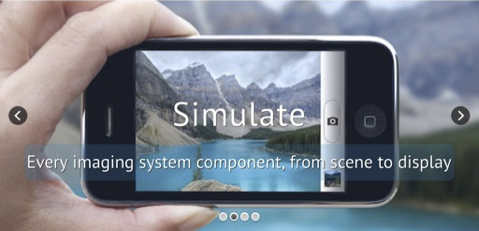
\includegraphics[width=0.8\textwidth,height=\textheight]{chapters/images/front-simulate.png}
\end{center}

\bookmarksetup{startatroot}

\chapter{Preface}\label{sec-preface}

Advances in image systems technology over the past few decades have
profoundly reshaped our world. Cameras are now ubiquitous, carried and
used by individuals daily. Security cameras are a common sight in public
spaces, while medical facilities rely on a variety of imaging systems,
from cameras to microscopes, for diagnosis and treatment. Modern
automobiles incorporate numerous cameras for enhanced safety, both
within the vehicle and for monitoring the surrounding environment.
Furthermore, intelligent systems now interpret and generate images,
demonstrating the growing sophistication of the field. Image systems
engineering has transitioned from a specialized domain dominated by a
few large corporations to a vast and intricate discipline with diverse
applications.

This book aims to serve as a resource for both newcomers and seasoned
professionals in the image systems engineering field. If you are new to
image systems, I hope this text provides a clear and welcoming
introduction. For those already experienced in imaging principles, I
understand the challenge and excitement of keeping pace with the rapid
technological evolution. This book is designed to serve as a useful
reference for aspects of image systems outside your primary area of
expertise.

A comprehensive understanding of an image system requires knowledge of
the original signal (the scene) and the system's parts: optics, sensors,
image processing, and display. In many applications, such as color
reproduction, knowledge of the characteristics of the human visual
system are also crucial. This book introduces tools for simulating the
performance of entire image systems, accounting for the properties of
each individual component.

No textbook, even one designed for online updates, can fully capture
every emerging technology. This book focuses on the enduring principles
that underlie each component of an image system. We use contemporary
technologies as illustrative examples, but our core objective is to
elucidate the fundamental concepts that remain relevant despite
technological advancements. Therefore, this book is titled:
\textbf{Foundations of Image Systems Engineering}.

\section{Why we wrote this book}\label{why-we-wrote-this-book}

Writing a textbook is a humbling experience. The Internet is filled with
wonderful resources on many topics, and it is clear to any reasonable
author that there are excellent online resources that cover some of the
same material. So, why write a book at all? After twenty years of
teaching this material, there are three main reasons we felt that
writing a book is worth the considerable effort.

First, asking a student to use material distributed across the Internet
produces an awkward learning experience. There can be many reasons to
understand any of these topics, and the Internet resources often connect
to some application. For example, image sensors might be used an example
circuit design or material science. Optics might be explained to support
biological microscopy. These different goals mean the ideas are
explained in different ways. Each video or web page reference is written
with a different voice and with different assumptions about the reader's
background and goals. This book aims to cover many topics in image
systems engineering clearly, and importantly we want to explain the
\textbf{connections} between a diverse array of technologies: measuring
light, analyzing and designing optics and electronic image sensors,
reproducing and displaying images, evaluating image quality, and using
image data to make inferences about the world.

Second, we would like to help the reader apply these ideas in his or her
work. The field of image systems engineering is sufficiently advanced
that we can often compute from the input (scene) to the sensor data.
Such simulations are enabling because the sensor data are the basis for
the software that calculates a displayed image, or the algorithm that
interprets the contents of the sensor data. Once the sensor data are
known, the simulation is simply a matter of software that is easily
shared. Predicting the sensor data from the light field in the scene is
the foundation for further analysis. It is challenging to build a
simulation of an image system, and we include software that the user can
use and build upon. Specifically, we provide open-source software tools
that we hope will make it easy for the reader to learn the principles
and also to experiment with different hardware designs and
post-processing algorithms. We illustrate the software by including code
snippets throughout the book, including links to runnable scripts.

A third reason we write this book is to tell the story of image systems
development. Images are very important to people, and a great many
scientists and engineers have contributed ideas and technologies to
acquire, render, and analyze images. We find the stories about the
people who made discoveries, or invented technologies, to be
fascinating. It is our hope that this book communicates how science and
engineering are very human activities, involving personalities, ideas,
conflicts, and friendships. Each year we teach the course, it feels like
we are visiting with the people who developed the field and trying to
understand what they were thinking at the time they made their
contributions. Their stories have inspired us to work in image systems,
and we hope some of our readers will be inspired, too.

\begin{tcolorbox}[enhanced jigsaw, bottomtitle=1mm, titlerule=0mm, arc=.35mm, colbacktitle=quarto-callout-note-color!10!white, coltitle=black, toprule=.15mm, bottomrule=.15mm, breakable, colframe=quarto-callout-note-color-frame, left=2mm, opacityback=0, colback=white, title=\textcolor{quarto-callout-note-color}{\faInfo}\hspace{0.5em}{Discovery and context}, opacitybacktitle=0.6, toptitle=1mm, rightrule=.15mm, leftrule=.75mm]

\section{Intellectual atmosphere}\label{intellectual-atmosphere}

``The History of Science has suffered greatly from the use by teachers
of second-hand material, and the consequent obliteration of the
circumstances and the intellectual atmosphere in which the great
discoveries of the past were made. A first-hand study is always
instructive, and often . . . full of surprises.'' (Ronald A. Fisher, in
(Bennett 1955))

The great and influential statistician, Ronald Fisher, wrote this
comment in 1936, though it was published much later by his estate. He
believed that the experiments reported by Mendel included some
improperly collected or analyzed data. He urges us to make the
distinction between secondary reporting of findings and fully
appreciating the context and intellectual mieliu of the original work.
His commentary goes back to the history in a thoughtful way.

In my view, this is too much to ask of all teachers at all times. But it
is not too much to ask of some of us. I should add that having now read
several of Fisher's original papers, and I am aware of his context
including some views that I find entirely wrong (Project Muse). I find
him and the world he represents a bit terrifying. But the importance of
his contributions cannot be ignored.

\end{tcolorbox}

This is an introductory book; each of the topics we cover can be studied
in much greater depth. Throughout we provide the reader with external
links to additional material, and in some cases we link to videos or
text that explain an idea or a specific technology in greater detail. We
hope you find that the value of this book is how it provides a
consistent thread connecting the material at the foundations of image
system. We hope this treatment is a good way to welcome people - whether
students at school or a new team member in a commercial venture - to the
exciting field of image systems. We hope you come away with tools to
help you do your own work, and with some understanding of the people and
ideas who have brought us this far.

\section{History of image systems}\label{history-of-image-systems}

\subsection{The first images}\label{the-first-images}

Capturing and reproducing images has been exciting to people for a long
time. In 1826, Joseph Nicéphore Niépce recorded the first film image,
the ``View from the Window at Le Gras''. He used the simplest optics: a
pinhole (camera obscura). The color in the rendering was a consequence
of the processing, and not an accurate representation of the scene
itself. The spatial pattern was blurry, and barely interpretable - but
it was inspirational. By 1840, Daguerre and then Talbot improved upon
the film chemistry to enable the first commercially viable monochrome
film.

\begin{figure}

\centering{

\includegraphics[width=0.4\textwidth,height=\textheight]{chapters/images/preface/ViewFromWindowLeGras-OriginalRotated.png}

}

\caption{\label{fig-window-le-gras}The first recorded image (``View from
the Window at Le Gras''). This monochrome image was made by Joseph
Nicéphore Niépce.}

\end{figure}%

By 1860 James Clerk Maxwell, in a masterful set of experiments and
analyses, had quantified the key properties of human wavelength
encoding. The principles and experiments from his work remain the
foundations of modern color science. In collaboration with Thomas
Sutton, Maxwell created the first color image. The image shows a colored
Tartan ribbon. Maxwell went on to other matters - such as clarifying the
connection between electricity and magnetism and showing that light is
an electromagnetic wave. Wow. He performed the work on color in his
mid-twenties. He died at 48 years of age, from the same type of cancer
that took his mother.

\begin{figure}

\centering{

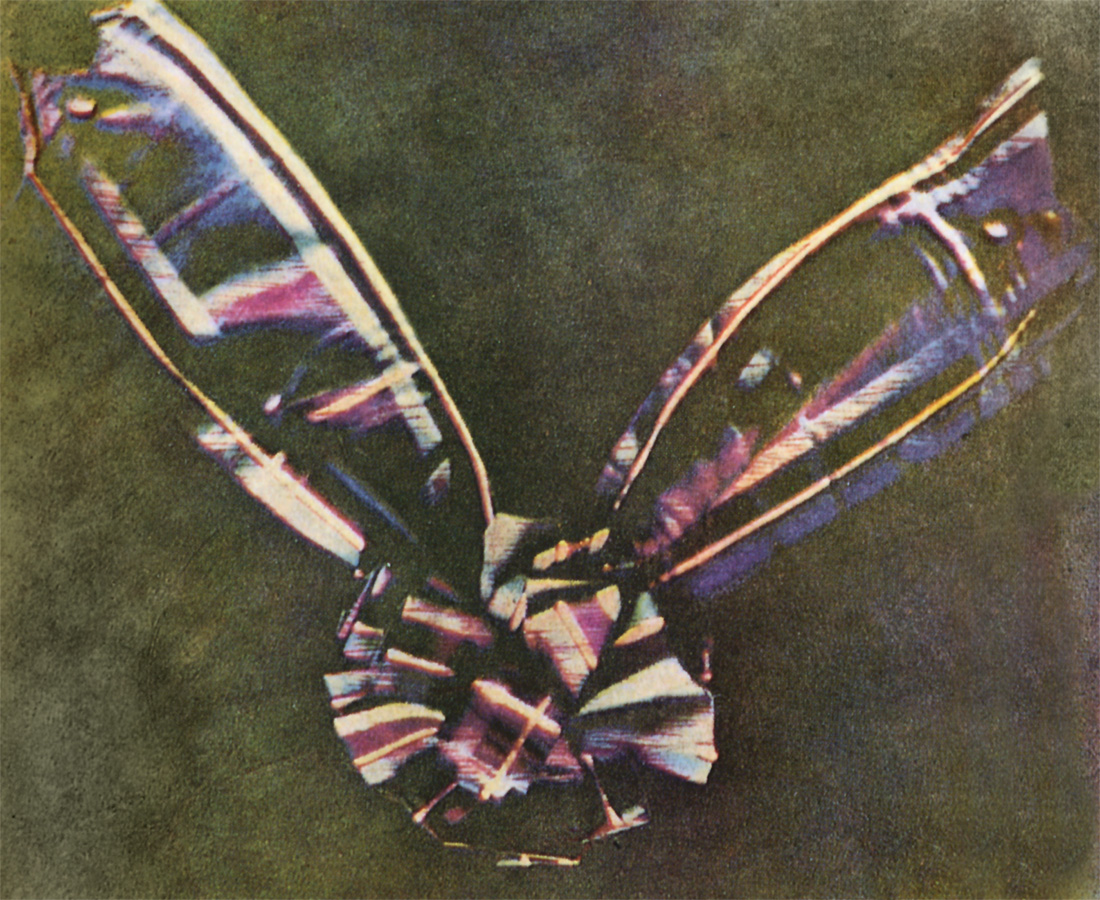
\includegraphics[width=0.4\textwidth,height=\textheight]{chapters/images/preface/Maxwell_Sutton_Tartan_Ribbon.jpg}

}

\caption{\label{fig-maxwell-sutton}The first color image was produced by
Thomas Sutton and James Clerk Maxwell. The image system for color was
based on principles of human color vision that were established by
Maxwell.}

\end{figure}%

\subsection{Chemical imaging}\label{sec-preface-film}

In 1888 George Eastman invented and commercialized a camera that used
rolls of film, enabling users to capture multiple images in a
convenient, handheld device (Figure~\ref{fig-film}). To take a picture,
shutter was opened and a lens formed an image on the film. The light
changed the molecules in the film layers. For color film, there were
multiple layers that differed in their wavelength sensitivity. Using
chemical processes, the density of changes to the light-sensitive
molecules could be measured and transferred to other media, such as
prints. This process required a variety of chemical consumables, and the
film could not be reused.

Eastman's company, Kodak, controlled the consummables and methods for
developing the roll of film into a series of pictures. Simplifying film
development was critical for the widespread adoption, and the company's
control of the consummables made them a huge commercial success.
Specialized labs processed the film and printed the image.

\begin{figure}

\centering{

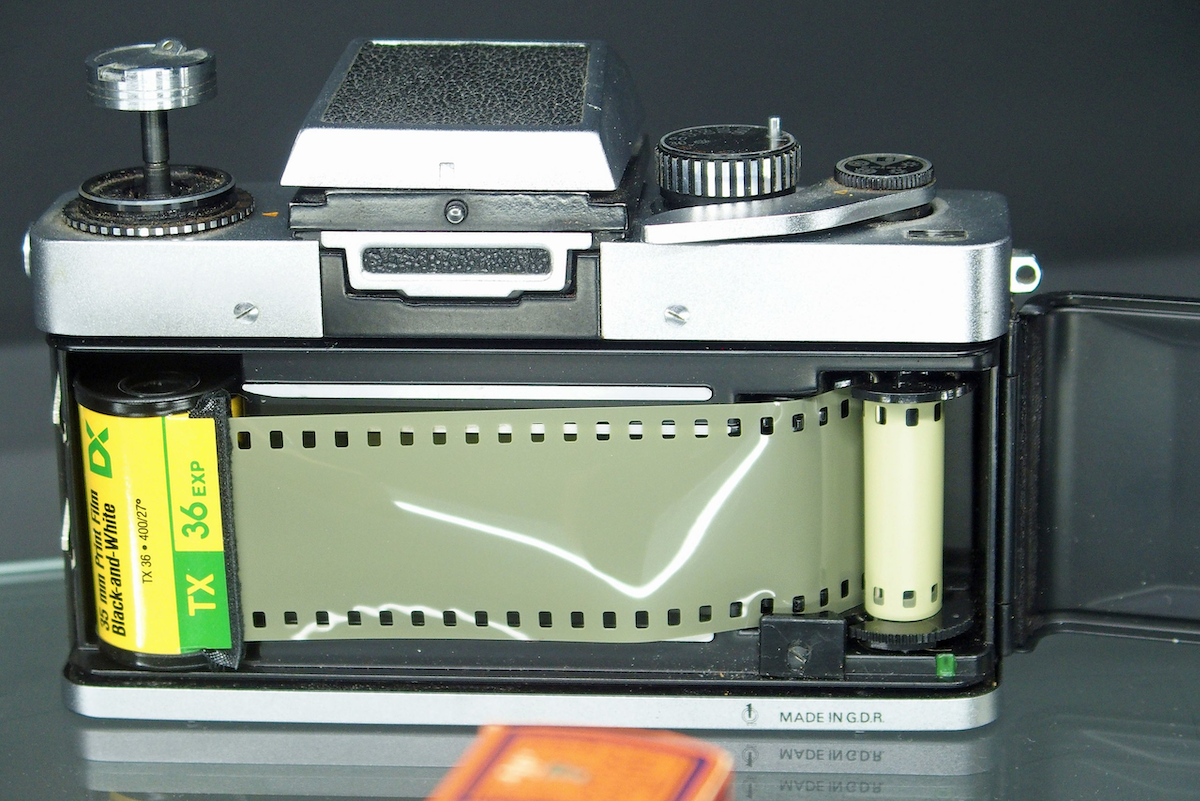
\includegraphics[width=0.6\textwidth,height=\textheight]{chapters/images/preface/film.png}

}

\caption{\label{fig-film}Film was the dominant image sensor and
recording material for a hundred years. The chemistry of film for both
encoding and developing into images was the core scientific discipline.
Film could not be reused, producing a steady commercial profit for large
companies, such as Kodak, Fuji, Polaroid and Agfa.}

\end{figure}%

The delay between acquiring a picture and seeing it printed was usually
days, or even weeks. Most of us would like to see the reproduction
quickly. In 1948 Edwin Land created a chemical process for rapidly and
developing the film on the spot, without going to a lab. His company,
Polaroid, was also a huge success. Though, the quality of the Polaroid
pictures was not equal to the quality of the pictures produced through
the slower developing film produced by Kodak, Fuji, and Agfa.

People were passionate about their film cameras, and taking pictures was
a common part of the family holiday and other special occasions. Images
with Kodak film dominated the market and its brand was dominant. Film
and the chemistry needed for film development required consumables,
which made the technology expensive but also profitable. The ability to
store the pictures, typically in photo-albums, was effortful but also
became part of many family's meaningful history. Editing pictures was
difficult, and thus not a thing - apart from propagandists. The
reproduction process included many nonlinear and adaptive steps, so that
the ability to perform quantitative image analysis was very limited.

\subsection{Electronic imaging}\label{electronic-imaging}

In 1970 Willard S. Boyle and George E. Smith at Bell Labs described an
entirely different approach to image capture: an image sensor based on
semiconductor technology (Boyle and Smith 1970; Boyle and Smith 1971).
Their invention was called a charge-coupled device
(\href{https://en.wikipedia.org/wiki/Charge-coupled_device}{CCD}) based
on Metal Oxide Semiconductor (MOS) circuitry. This light sensor
revolutionized the field of imaging by enabling a new way of recording
the electromagnetic radiation. There are no consumables when acquiring
images with a solid-state sensor. The digital output of the sensor made
it straightforward to integrate image acquisition with computers, which
simplified storing, sharing, editing and analyzing images. A new
business model was required \footnote{Kodak and Polaroid did not adapt
  and both ultimately reorganized under bankruptcy. At this time, their
  principal function is to market their brand name. Fujifilm, an
  excellent but late entry into the film market, adapted and has a
  relatively high valuation and a broad range of products.}.

\begin{figure}

\centering{

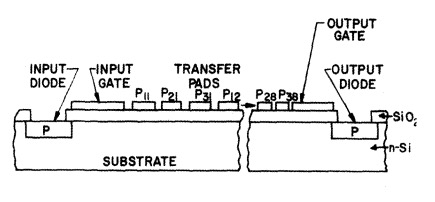
\includegraphics[width=0.5\textwidth,height=\textheight]{chapters/images/preface/tompsett-circuit-1970.png}

}

\caption{\label{fig-tompsett}From Tompsett et al. (1970). This was first
CCD implementation, for a shift register. The first patent for an imager
was Tompsett (1978).}

\end{figure}%

At first, cameras based on CCDs replaced film in a few specialized
applications: science and engineering for telescopes, and microscopes.
The power requirements of CCDs, which was necessary for the method of
reading out the data, made CCDs impractical for lightweight consumer
cameras.

In 1993 this changed with Eric Fossum's invention, at the Jet Propulsion
Labs in Pasadena, of a solid state sensor based on CMOS. Shifting from
MOS to CMOS enables the sensor to operate with much lower power
requirements (Fossum 1993; Fossum et al. 1995). The first CMOS sensors
were noisy and low resolution compared to the CCDs - which had a 25 year
head-start! But engineering efforts led to commercial CMOS imagers with
excellent sensitivity, low noise, and low power. By 2020 about 200 CMOS
image sensors were built every second, and 6 billion were sold per year
(Fossum 2023). Today, about 7 billion people carry a smartphone with one
or more CMOS sensors, most of these people keep the camera in a pocket
or purse throughout the day. These sensors record still and video
digital image sequences. The raw image data are immediately transformed
by computer algorithms, can be viewed immediately, stored in digital
memory, and easily edited, shared or analyzed. We have gone from the
first electronic imager to worldwide adoption in 50 years.

The sensor advances spurred the development of other hardware components
of image systems. Many of these changes arose because the system needed
to fit within the slim form factor of the phone. New optics were
designed and new displays for viewing the image prior to capture also
evolved. There were also many new digital image processing methods.
Semiconductor imaging, integrated with a computational system, has
become a massive industry of image processing applications.

\section{Image systems and human
vision}\label{image-systems-and-human-vision}

The important 20th century vision scientist, William Rushton, wrote -
``You will need no words of mine to convince you how precious are your
eyes.'' Understanding how the eye encodes light, and how the brain
interprets this encoding, is important for understanding many aspects of
human behavior. Vision helps with many of life's critical activities:
moving from place to place, interpreting a facial expression, selecting
food, reading a page.

When we design, build, or analyze image systems, we must account for how
the signals are encoded and also how they will be used. For the very
large application of consumer photography, it is essential to have a
model that accounts for the system that will receive the image: the
human visual system. As we shall see, many components of the image
systems, including color filter arrays in sensor and image compression
strategies in digital coding, are designed to account for the properties
of the human visual system.

Image systems designed for other purposes, such as automotive or
robotics sensor, also use a general principle that was proposed as the
basis of human vision. The great 19th century scientist, Hermann von
Helmholtz, proposed that the brain uses the image encoded by the eye to
make an inference about the properties of the scene.

\begin{figure}

\begin{minipage}{0.70\linewidth}

\begin{quote}
The general rule determining the ideas of vision that are formed
whenever an impression is made on the eye, is that~such objects are
always imagined as being present in the field of vision as would have to
be there in order to produce the same impression on the nervous
mechanism (von Helmholtz 1925, Vol III, p.~2, Italics in the original)
\end{quote}

\end{minipage}%
%
\begin{minipage}{0.30\linewidth}
\includegraphics{chapters/images/preface/helmholtz-wikipedia.png}\end{minipage}%

\end{figure}%

This is an important principle for most modern image systems
applications, as well. A robot uses image data to infer the location and
orientation of a package on the table; a microscopist uses image data to
infer the properties of cells in a biopsy. An autonomous vehicle uses
image data to identify nearby traffic. A camera on an assembly line
assessing part quality makes an inference between the materials and
structures. The early pioneers in imaging systems developed the means of
encoding the light - optics, film, sensors. The modern pioneers are
expanding these technologies and coupling the acquired images with
powerful new algorithms that interpret the encoding with respect to the
specific properties of the scene.

\section{About this book}\label{about-this-book}

This book is divided into three sections: image formation, sensor
encoding, and image processing. Within each section we introduce the
foundations, and then we illustrate these principles with
implementations in different contexts that have different requirements.
For example, the size requirements on optics differ between a cell phone
and a telescope. The power requirements for an image sensor differ
between an endoscope and a camera on an assembly line. For consumer
photography applications the human visual system is an essential
context, but not for a camera used to guide an automobile. The diversity
of applications - and the ability to match the physics to these
applications - make the field of image systems engineering interesting.

\section{Image systems engineering at
Stanford}\label{image-systems-engineering-at-stanford}

The book is based on a course that Professor Brian Wandell and Dr.~Joyce
Farrell have been teaching for over twenty years. Stanford's involvement
in the image systems engineering accelerated in the early 1990s. At that
time Farrell was leading a group at Hewlett-Packard Laboratories (HPL),
and imaging was a relatively new direction for HP. The company had
developed a type of printing technology (inkjet), and they were starting
to build image capture devices based on flatbed scanners. Wandell worked
at Stanford, an institution that encouraged collaborations with
industrial partners, and his focus was on human visual perception,
particularly color. The reproduction of images depended on basic
knowledge of human visual perception, and members of the HP staff needed
to hire people to design and evaluate new types of image systems.

Dr.~Farrell thought that Stanford might set up an image systems
engineering training program to provide a source of new employees. She
approached Professor Joseph Goodman and Professor Brian Wandell,
suggesting that they initiate such a training program. Professor John
Hennessy, who was Dean of the School of Engineering at the time,
encouraged us to go ahead, and so we did (Goodman and Wandell 1996).
After a few years, Farrell moved from HP to Stanford to become executive
director and Professor Bernd Girod joined Stanford and became the
faculty director. Together, they transformed the training program into
an industry affiliates program,
\href{https://scien.stanford.edu/}{SCIEN}. For twenty-five years this
organization served as a watering hole where skilled engineers and
scientists have met for talks and conferences about new developments in
image systems. Many of the talks from that seminar series are available
to
\href{https://scien.stanford.edu/index.php/events/scien-seminars/}{view
online}.

Around that time
\href{https://profiles.stanford.edu/abbas-el-gamal}{Professor Abbas El
Gamal} returned to Stanford from industry. Along with Dr.~Boyd Fowler,
he chose to explore novel circuit designs in CMOS imagers, extending the
work initiated by Eric Fossum at JPL. El Gamal and Wandell met regularly
with their group to discuss how different sensor designs might produce
images with extended dynamic range. As we set about raising funds to
support the students, postdocs and research costs, we encountered the
same resistance that Eric Fossum mentions (see above). Responding to
that resistance was fun and sharpened our thinking.

The collaboration between engineers and psychologists included people
with a diverse set of skills. We all had some comfort with basic
electrical engineering mathematics, but there were many specializations
related to imaging and visual perception. That is, the physics and
biology represented by the mathematical models were not part of an
existing Stanford course curriculum. The research, which included sensor
tapeouts, calibration, image display, required that we communicate with
precision. This led us to create software that forced us to be very
explicit about what we meant. This same software could also be used to
try out new ideas before going to the trouble and cost of building the
system. Image system simulation remains an important concept, and these
days the idea applied broadly to many types of systems is often called a
`digital twin'.

Others in the imaging industry also needed tools to communicate between
team members building image systems: These teams included experts in
optics and sensors, or experts in sensors and displays. The software
helps engineers understand how varying the specifications of individual
imaging components will impact overall system performance. The
simulation software was initially developed by Ting Chen and me, with a
focus on the sensor. Its scope grew extensively to model the input
(three-dimensional spectral radiance of scenes) various types of optics,
and the control systems that manage image acquisition. With the
assitance and comments from students and commercial collaborators over
the years we now have a suite of tools that have been numerically
validated. The tools include a core library of functions that emphasize
physical descriptions of scenes, optics, sensors, displays, and color
metrics. We call these tools the Image Systems Engineering Toolbox. We
use that software in courses, and we will use it in this book.

Stanford is a teaching institution, although there are times we are
distracted by other pursuits. The research we do is closely coupled to
the courses that we teach, and before long Dr.~Farrell and Professor
Wandell initiated a course called `Image Systems Engineering.' The
course mission is to teach students about the foundations of image
systems engineering; these are the ideas that will apply to all image
systems even as technology implementations evolve. For example, we think
that understanding the physics of the scene is essential for
implementing an image system. Certain principles of optics will remain
essential, as well as critical ideas about image processing, and
displays even as technology evolves. Perhaps more than most, we also
think that understanding how the human visual system encodes color,
adapts to changing environmental conditions, and judges position and
sharpness will be fundamental for many image systems.

This book is a summary of what we have learned, and what we teach, in
our image systems course. To help students understand the concepts and
calculate practical examples, we use the Image Systems Engineering
Toolbox for Cameras
(\href{https://github.com/iset/isetcam/wiki}{ISETCam}). This software
package enables a large variety of calculations starting with the light
in the scene, calculating through the optics, arriving at the sensor,
and then processed for either visualization or machine learning
applications. The entire repository is open and extensively documented.
Additional repositories that (a) use graphics tools to create
three-dimensional spectral scenes
(\href{https://github.com/iset/iset3d-tiny/wiki}{ISET3d}), and (b) model
details of human vision
(\href{https://github.com/isetbio/isetbio/wiki}{ISETBio}), are also
open-source and available. These respositories build on the tools in
ISETCam.

\part{Scenes}

\chapter{Light and seeing}\label{sec-light}

\section{Light and seeing overview}\label{sec-light-overview}

Electromagnetic radiation fills the world around us, providing a rich
and reliable stream of information. Mobile organisms --- whether a hawk,
a rabbit, or a human --- have implemented ways to record and interpret
this information. They use the radiation to make decisions and generally
interact with their surroundings. We call the sensing and interpretation
of the radiation \textbf{visual perception} or more simply,
\textbf{seeing}.

Visual perception is fundamental for guiding movement, enabling animals
to locate resources, avoid threats, and navigate their environments. The
use of radiation for mobility and decision-making by mobile organisms is
in contrast to immobile life forms, such as trees and plants. For these
organisms the ambient radiation serves primarily as a source of energy,
rather than information.

In robotics and most computer applications, visual sensing serves a
similar purpose: to enable actions and movement within dynamic and
complex environments. Robots with imaging systems identify and
manipulate parts. Cars with image systems navigate through their
surroundings. Medical imaging provides diagnostic information to guide
interventions. For both artificial and biological systems image systems
provide information that enables goal-oriented actions.

\begin{tcolorbox}[enhanced jigsaw, bottomtitle=1mm, titlerule=0mm, arc=.35mm, colbacktitle=quarto-callout-note-color!10!white, coltitle=black, toprule=.15mm, bottomrule=.15mm, breakable, colframe=quarto-callout-note-color-frame, left=2mm, opacityback=0, colback=white, title=\textcolor{quarto-callout-note-color}{\faInfo}\hspace{0.5em}{Who needs a brain?}, opacitybacktitle=0.6, toptitle=1mm, rightrule=.15mm, leftrule=.75mm]

The deep connection between mobility, visual sensing, and the brain is
illustrated by the remarkable life path of the
\href{https://movementum.co.uk/journal/sea-squirts}{sea squirt}. It
begins life as tadpole-like larvae, equipped with a brain and a tail for
swimming. Once the tadpole finds a suitable spot to settle, it attaches
to a hard surface like a rock or coral and becomes immobile.

As soon as the sea squirt fixes itself to the rock, with no more
navigation or swimming, its brain is no longer needed. In a truly
bizarre twist, the sea squirt digest its own brain. This adaptation
reallocates energy resources from the now unnecessary brain to more
vital functions.

\begin{figure}[H]

\centering{

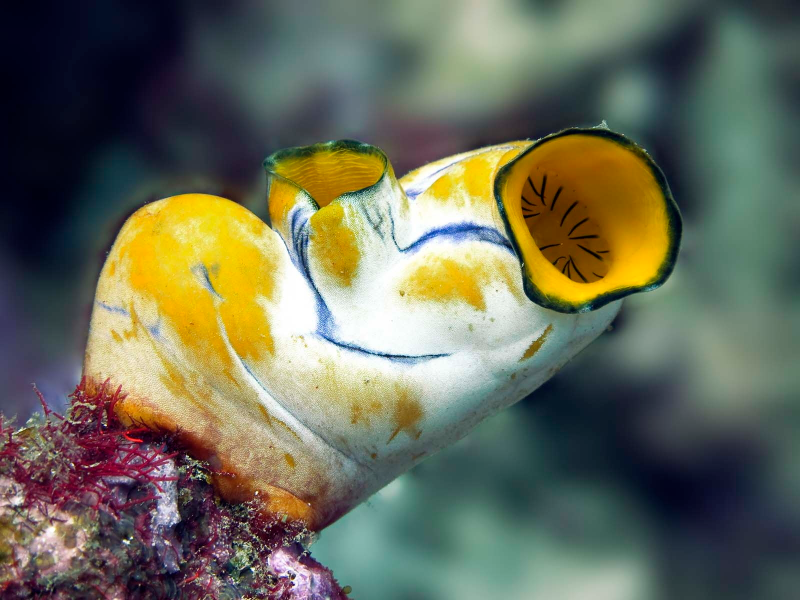
\includegraphics[width=0.5\textwidth,height=\textheight]{chapters/images/lightfields/01-lightfields/seasquirt.png}

}

\caption{\label{fig-seasquirt}A sea squirt image from
\href{https://goodheartextremescience.wordpress.com/2010/01/27/meet-the-creature-that-eats-its-own-brain/}{this
nice site}. This one is from Papua New Guinea. Plenty more images (and
sea squirts) over there.}

\end{figure}%

My Stanford colleague, Irv Weissmann, and his group wrote many papers
about neurodegeneration using the sea squirt.

\end{tcolorbox}

Consumer photography - a large and important image system application -
is an important exception. Consumer photographs are created to store
memories and evoke emotions, not to guide navigation or immediate
decisions. As I discuss in later chapters, the technologies for
evaluating consumer photography differ from standard engineering metrics
because of their heavy reliance on the properties of human perception.

In summary, some image systems measure electromagnetic radiation because
the signal is useful for movement or interacting with objects. Other
image systems measure radiation to record a moment, enabling us to
reproduce the signals at a later time. And finally, some image systems
measure electromagnetic radiation at wavelengths we do not see, enabling
us to explore domains that are beyond our senses \footnote{There are
  instruments that use different wavebands of the electromagnetic
  spectrum. \href{resources/lightfields-wavebands.html}{A brief
  introduction is here.}. More examples of instruments will be presented
  in later chapters.}. This section of the book is devoted to
understanding the signal.

\section{Light and the electromagnetic
spectrum}\label{sec-light-em-spectrum}

One of the great achievements of science is the realization that
seemingly different phenomena are deeply connected. By the early 1800s,
scientists had uncovered links between electricity and magnetism:
Øersted (1820) showed that electric currents generate magnetic fields,
and Faraday (1832) demonstrated that changing magnetic fields induce
electric currents.

James Clerk Maxwell unified these discoveries in a set of mathematical
equations now known as \textbf{Maxwell's equations}. He demonstrated
that oscillating electric and magnetic fields behave as waves that
propagate through space. Remarkably, the predicted speed of these waves
matched the measured speed of light. Maxwell concluded that light itself
is an electromagnetic wave, thereby uniting electricity, magnetism, and
optics into a single theoretical framework: electromagnetic radiation
spanning a range of wavelengths.

Not all electromagnetic wavelengths are equally useful for vision. The
human eye detects electromagnetic radiation within a specific range,
approximately 380 nm to 770 nm. This range is referred to as
\emph{light}---electromagnetic radiation that is visible to the human
eye. Radiation in this range is particularly useful for vision because
it is strongly absorbed and reflected by objects in the environment,
making it ideal for detecting and interpreting the world around us.

In contrast, high-energy radiation, such as X-rays (0.01--10 nm) and
gamma rays (\textless{} 0.01 nm), tends to pass through most objects
without significant interaction. On the other end of the spectrum,
low-frequency radiation (\textgreater{} 1500 nm) provides lower spatial
resolution and is heavily influenced by thermal effects, limiting its
utility for detailed imaging. The visible spectrum occupies a unique and
advantageous position for vision and perception.

\section{The environmental light field}\label{sec-lightfields-types}

Electromagnetic radiation fills the environment, traveling in many
directions and often interacting with materials. We call the
environmental radiation field in the visible wavelength band the
\emph{environmental light field}.

Leonardo Da Vinci's notebook (Da Vinci 1970) describes why he concluded
that light fills the environment. He placed a small hole in a wall of a
windowless room that was adjacent to a brightly illuminated piazza
(Figure~\ref{fig-ayscough}). This produced an (inverted) image of the
piazza on the wall within the room. Leonardo observed that one can place
the pinhole anywhere in the wall and an image of the same objects is
produced. He concluded that the light field is ``all everywhere and all
in each part''\footnote{\textbf{PROVE HOW ALL OBJECTS, PLACED IN ONE
  POSITION, ARE ALL EVERYWHERE AND ALL IN EACH PART} ``I say that if the
  front of a building---or any open piazza or field---which is
  illuminated by the sun has a dwelling opposite to it, and if, in the
  front which does not face the sun, you make a small round hole, all
  the illuminated objects will project their images through that hole
  and be visible inside the dwelling on the opposite wall which may be
  made white; and there, in fact, they will be upside down, and if you
  make similar openings in several places in the same wall you will have
  the same result from each. Hence the images of the illuminated objects
  are all everywhere on this wall and all in each minutest part of it.
  The reason, as we clearly know, is that this hole must admit some
  light to the said dwelling, and the light admitted by it is derived
  from one or many luminous bodies. If these bodies are of various
  colours and shapes the rays forming the images are of various colours
  and shapes, and so will the representations be on the wall.
  (Leonardo's 1509 Notebook, curated by John Paul Richter)''}.

\begin{figure}

\centering{

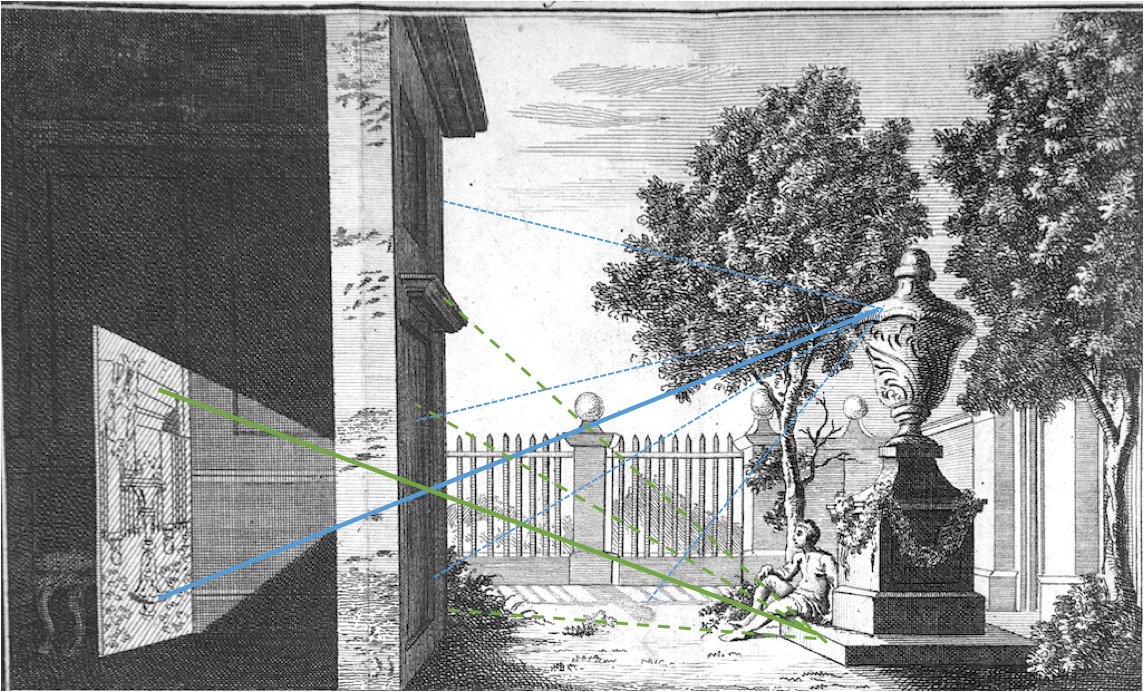
\includegraphics[width=0.95\textwidth,height=\textheight]{chapters/images/lightfields/01-lightfields/Ayscough-1755-small-wikipedia.png}

}

\caption{\label{fig-ayscough}Ayscough's book Ayscough (1755) (``A short
account of the eye and nature of vision. Chiefly \ldots{} to illustrate
the use and advantage of spectacles'') opens with this illustration of
Da Vinci's pinhole camera. I superimposed the colored lines to indicate
the courtyard light rays, emitted in all directions. The solid lines are
selected by the pinhole and form the image in the dark room. The full
collection of rays, solid and dotted, represents the \emph{environment
light field}.
\href{https://en.wikipedia.org/wiki/Camera_obscura\#/media/File:1755_james_ayscough.jpg}{Source:
Wikipedia Camera Obscura}.}

\end{figure}%

For the moment, it is convenient to consider the light field as
comprising a large set of rays. We can describe the light field in the
environment, \(L_E\), by the intensity of each ray, expressing the
intensity as an explicit function of its various parameters. At each
point in the volume of space, \((x,y,z)\), there are rays traveling in
many directions. We specify these directions by two direction angles
\((\alpha,\beta)\), the azimuth and elevation. Each ray has wavelength
\(\lambda\) and polarization \(\rho\). The ray intensities are described
by the function:

\[
L_E(x,y,z,\alpha,\beta,\lambda,\rho)
\]

People in many fields are familiar with the concept of the light field,
but they use different terminology. Physicists often describe the
environmental light field as the spectral radiance of the environment
(see this \href{https://youtu.be/FjHJ7FmV0M4?si=wi2twZVYjF9KJGRY}{lovely
description from Feynman}). The general \emph{light field} terminology
was introduced into optical engineering by Gershun (1939) as part of his
work in understanding how to design lighting environments, such as the
lighting in school rooms and public places\footnote{I enjoyed the first
  sentence in the 1939 translation of Gershun's (1939) paper. The
  translators, Moon and Timoshenko, express frustration with the pace of
  advances in photometry. ``Theoretical photometry constitutes a case of
  `arrested development', and has remained basically unchanged since
  1760 while the rest of physics has swept triumphantly ahead.'' Gershun
  himself expresses the same sentiment: ``The problems of theoretical
  photometry were pushed aside from the main path of the development of
  physics.''}. Ted Adelson and Jim Bergen (1991) used the term
\emph{plenoptic function} to describe the same idea\footnote{Adelson and
  Bergen (1991) introduced the plenoptic function for a pinhole camera
  and a sensor, making it more closely related to the incident light
  field. (Section~\ref{sec-incident-lightfield}). They explained it
  using a pinhole camera model, so that the two parameters describing
  the aperture position were not needed. With these restrictions, the
  plenoptic function is equivalent to the spectral irradiance at the
  image sensor (Wandell and Brainard 2021). The authors clearly had the
  idea of the environmental and incident light fields in mind.}. The
great value of the light field concept in computer graphics was
explained by Marc Levoy and Pat Hanrahan (1996). I will use the light
field terminology because I find it more familiar and engaging than
spectral radiance, electromagnetic radiation, or plenoptic.

\section{Incident light field}\label{sec-incident-lightfield}

An imaging system, say the eye or a pinhole, records only the portion of
the environmental light field that arrives at its entrance pupil
(Figure~\ref{fig-incident-lightfield}). It is worth distinguishing that
part of the environmental light field with a name: \emph{incident light
field}.

\begin{figure}

\centering{

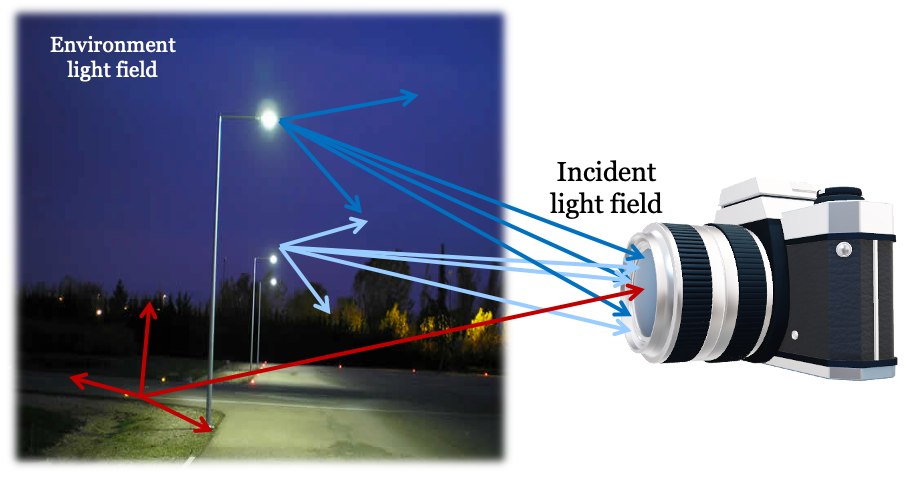
\includegraphics[width=0.8\textwidth,height=\textheight]{chapters/images/lightfields/01-lightfields/01-incident-lightfield.png}

}

\caption{\label{fig-incident-lightfield}The incident light field is the
subset of environmental light field rays that arrive at the image
systems' entrance pupil.}

\end{figure}%

The rays of the incident light field can be described with one fewer
parameter than the environmental light field because the entrance pupil
is just a two-dimensional surface. Thus, the three dimensional position
is replaced by the two-dimensional position in the entrance pupil,
\((u,v)\). We need, however, additional parameters to define the image
system: The aperture has a position in space \(\mathbf{p}\) and and a
viewing direction \(\mathbf{n}\). We include these as a side-condition
in the parameters that describe the ray intensities of the incident
light field

\[
L_I(u,v,\alpha,\beta,\lambda,\rho; ~\mathbf{p},\mathbf{n}) .
\]

To acquire full information about the environmental light field, we must
follow Leonardo and measure the incident light field at multiple
locations and directions. Many animals have two eyes and thus acquire
two simultaneous measurements of the light field. This has the benefit
of acquiring more information about the light field, as well as
providing one remaining eye in the case of disease or damage. Some
animals point the two eyes in very different directions and thus sample
the environmental light field very broadly (e.g., rabbits, and animals
that are prey). Other animals overlap the visual field of the two eyes
to acquire information useful for estimating distance (stereo vision,
animals that are predators). Even more information about the
environmental light field is measured, over time, as the head moves
heads and the eyes rotate (motion parallax).

Engineers have built camera arrays that capture more than two incident
light fields. Measuring from multiple positions and directions, enables
us to create displays that reproduce the experience of being in the
environment as a person changes position and direction of gaze. (If the
environment is unchanging, a single camera that moves around can be
used.) These systems rely on the principle Leonardo identified: the
light field is everywhere, and we can measure it by recording images at
many different positions using cameras at many positions and pointing in
many different directions.

A large, rectangular camera array to measure the light field was built
by my colleagues at the Stanford Graphics Lab (Levoy and Hanrahan 1996,
Figure~\ref{fig-camera-array}). The cameras measure multiple views; all
the cameras point in the same direction. Arrays with different camera
configuration, at the bottom of the figure, capture multiple directions
from a particular position. These camera arrays acquire enough
information so that we can render images that match what a person would
see if they look around. Camera arrays that acquire enough information
for both 360 deg and slightly different positions, sometimes called
stacked omnistereo, have also been built (Thatte et al. 2017). From
these data, along with an interpolation strategy, we can calculate
images from a range of viewpoints.

\begin{figure}

\sidecaption{\label{fig-camera-array}The Stanford Multi-Camera Array
(top) comprised 128 cameras that measured the environmental light field
from many positions. With this configuration one can recreate the
experience of moving side to side as well as back and forth. Other array
configurations (bottom) have cameras pointing outward from a point.
These capture the light field from many directions and can recreate the
experience of looking around the room from the point.}

\centering{

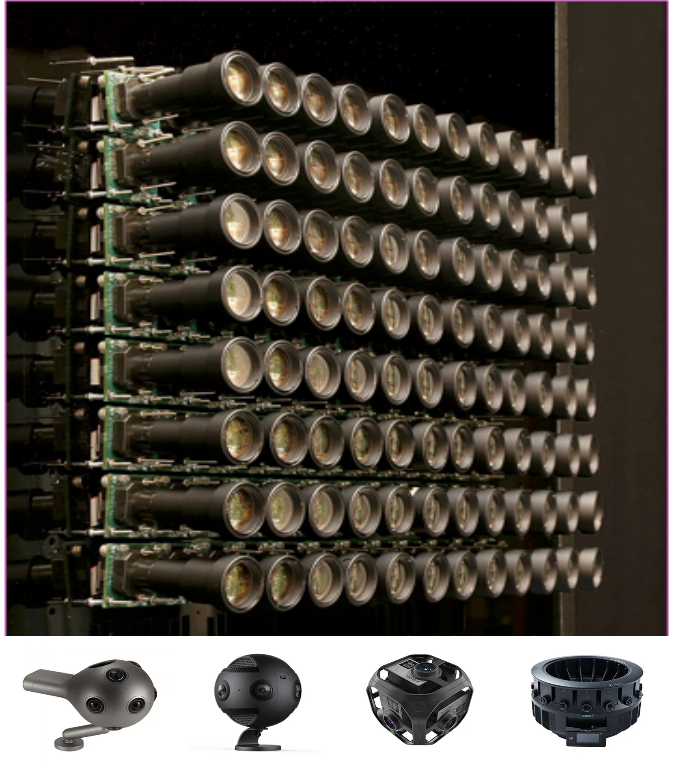
\includegraphics[width=0.7\textwidth,height=\textheight]{chapters/images/lightfields/01-lightfields/01-camera-array.png}

}

\end{figure}%

\section{Optical light field}\label{sec-optical-lightfield}

The image system optics, whether a pinhole, thin lens, or multi-element
lens, transforms the incident light field into a new light field within
the camera. This \emph{optical light field} exists between the exit
pupil of the optics and the sensor. The optical light field originates
in the environment, is reduced to the incident light field, and then
transformed by the optics. The camera sensor, or the retina, measures
the optical light field\footnote{Ng et al. (2005) used the phrase
  `in-camera light field.' I like that expression, too.}.

\begin{figure}

\sidecaption{\label{fig-optical-lightfield}The rays emerging from the
exit pupil of the optics are captured by the sensor (or film). These
rays form a light field within the camera, the optical light field
\(L_O\). The only rays of this light field that matter for the image
system are those that are captured by sensor.}

\centering{

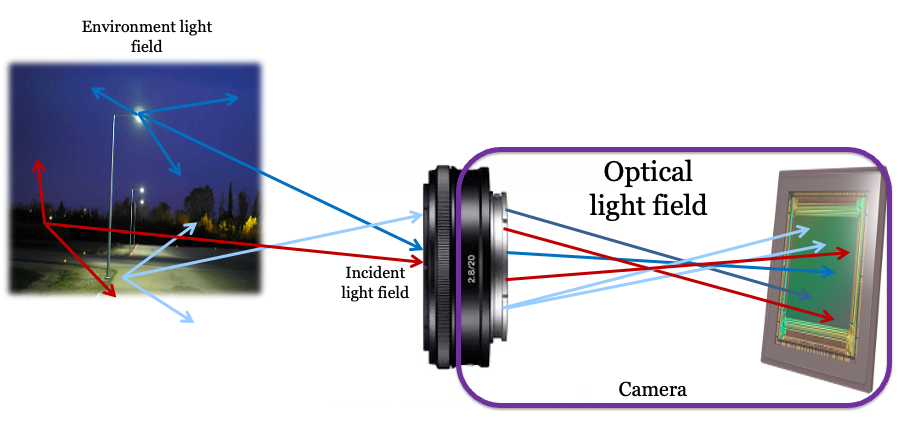
\includegraphics[width=0.8\textwidth,height=\textheight]{chapters/images/lightfields/01-lightfields/01-optical-lightfield.png}

}

\end{figure}%

The environmental and incident light fields use parameters of position
and angle for each ray. For the optical light field, however, we only
measure rays that arrive at the sensor (or film). It is helpful,
therefore, to parameterize the optical light field using two spatial
parameters: where the ray exits the lens (\((u,v)\)) and the position it
arrives at the sensor, \((w,z)\). These four spatial parameters
substitute for the positions and angles we use in the other light
fields. It is possible, of course, to convert the sensor position
parameters into angular parameters at the exit pupil.

\[L_O(u,v,w,z,\lambda,\rho)\]

The data recorded by the sensor is used to create a reproduction of the
image, or as information for interpreting the scene. The sensing and
perception systems that derive information from the light field are
designed to account for which information in the environmental light
field makes it all the way through to the optical light field.

The most common sensors in cameras record only partial information about
the optical light field. The rays arriving at a point on the sensor
surface are summed together, no matter where the ray exited the optics.
This type of sensor does not not preserve information about where the
rays arise in the exit pupil\footnote{Or, equivalently, they sum across
  the angles of the rays arriving at the sensor.}.

This implementation at the sensor is a decision, not a requirement.
Various authors pointed out that measuring more information about the
optical light field would enable us to know more about the environmental
light field. For example, Adelson and Wang (1992) built a camera that
measures the ray intensity at multiple angles at each location on the
sensor, and they used this information to estimate depth. Ren Ng's
company, Lytro, developed a commercial sensor to measure the optical
light field (Ng et al. 2005); they also developed algorithms to enable
users to refocus images or change the depth of field after capture. In
Section~\ref{sec-focus-control} I describe how modern sensors use light
field information for camera autofocus, and in
Section~\ref{sec-sensor-lightfield} I describe how light field sensors
capture a more complete version of the optical light field.

\section{Interpreting the light
field}\label{interpreting-the-light-field}

Encoding the light field data is a first step in seeing. A next step is
interpreting the measurements. The invention of algorithms that
interpret the light field is a central to building computers that see.
Discovering how the brain interprets the encoded signal is an important
part of vision science.

Building an internal model of the scene from the encoded light field has
long been believed to be what people do. Nearly two centuries ago by the
great vision scientist, Helmholtz, wrote:

\begin{quote}
The general rule determining the ideas of vision that are formed
whenever an impression is made on the eye, is that \emph{such objects
are always imagined as being present in the field of vision as would
have to be there in order to produce the same impression on the nervous
mechanism} {[}Italics in the original; Southall, Physiological Optics,
Vol. III, p.~2, 1865{]}
\end{quote}

Understanding the light field and the instruments that measure it will
help us achieve that goal.

\chapter{Measuring light fields}\label{sec-lfmeasurement}

\section{Measuring light fields -
overview}\label{sec-lfmeasurement-overview}

When we quantify the electromagnetic radiation, we are making a
\textbf{radiometric} measurement. The amount can be specified in units
of energy or the number of photons. If we measure how the amount over an
array of sampled locations, we are measuring an image. The image might
represent the radiation incident on a surface (such as a photograph) or
encoded by a sensor array. The title of this book, foundations of
\textbf{image} systems engineering, acknowledges the importance of
measuring light intensity as an image is central to the field.

Many aspects of image systems engineering are framed in terms of the
radiance image, rather than think about the radiation as rays or waves.
For example, suppose we measure the image at two planes: the plane just
prior to the optics and the plane just prior to the image sensor
surface. The relationship between these two images will depend upon the
optics, of course. We would like to model the transformation between
these two images; this transformation characterizes the optics.

As a second example, we may wish to know the light intensity emitted
from a display and the corresponding intensity that will arrive at the
eye. Or we may want to know how the intensity of radiance that is
incident on a surface, and the intensity of the radiance that is
reflected by the surface. These calculations do not require us to think
of rays or waves. We can develop tools and models based entirely on
measurements of intensities from radiance sensors.

The key principles for defining systematic measurement of image
intensities are from \textbf{Radiometry}, the field that specializes in
quantifying the light intensity at different positions. This section
introduces basic concepts of Radiometry, along with the standard units
used for quantifying the intensity. Radiometric units are an important
part of image representation in the ISETCam simulation software. In
Chapter~\ref{sec-optics-linear-space} we introduce models of the
intensity transformations, particularly for the important case of
characterizing optics. Those radiance calculations rely on the
properties of images and rely heavily on linear systems theory.

\section{Radiometric units}\label{radiometric-units}

Radiometric measurements are made separately for each wavelength. For
people working with light, wavelength is commonly expressed with respect
to nanometers \footnote{Units of micrometers (microns, \(\mu\)) are
  commonly used by people working in the infrared studies, units of
  angstroms in atomic and x-ray studies, and electron volts in
  high-energy photon research.}. We quantify the radiance by measuring
the amount of energy, or equivalently the number of photons, present at
a location. The basic energy unit is joules per second, (watts). In the
case of photons the basic unit is photons per second. Thus, in
radiometry one often finds units such as (watts per nanometer) or
(photons per sec per nanometer).

We describe the energy separately for each wavelength because, in most
cases, the energy at different electromagnetic wavelengths act
independently: we can measure the energy at two wavelengths separately,
mix the two lights, and the result is simply the sum of the individual
measurements. This additivity is a critical feature of light behavior in
many cases \footnote{There are important and useful cases light when
  radiance at one wavelength evokes emissions at other wavelengths
  (fluorescence). There are also important cases of non-linear behavior
  (e.g., two-photon imaging). We discuss these when we review special
  instrumentation.}.

Radiometry defines units that are helpful for different types of
geometry. The radiometric measures can be divided with respect to those
from a source (radiance) and those arriving at a surface (irradiance).
These can be further divided with respect to measures from a small
(point) source, or from an extended surface.

Finally, adjacent to the radiometric measurements there is a set of
units that summarize the impact of the radiation on the human visual
system. These measurements begin with the spectral radiometry units, and
they are then reduced by calculating a weighted sum across wavelengths.
The weights are selected to represent (roughly) the relative visibility
of each wavelength. These \textbf{photometric} units parallel the
radiometric units; for example, radiance and irradiance correspond to
luminance and illuminance. In this section, we will describe the
radiometric quantities.

The reader might consult
\href{https://wandell.github.io/FOV-1995}{Foundations of Vision} for
more information about human vision; a summary of critical aspects of
human vision for image systems engineering is presented in
Chapter~\ref{sec-human}. The experimental basis of photometry for the
weighted sum across wavelengths -the key step to spectral radiometric
quantities into photometric quantities- is explained in
\textbf{?@sec-human-imagequality}.

\section{Radiance from a point}\label{radiance-from-a-point}

\begin{figure}

\centering{

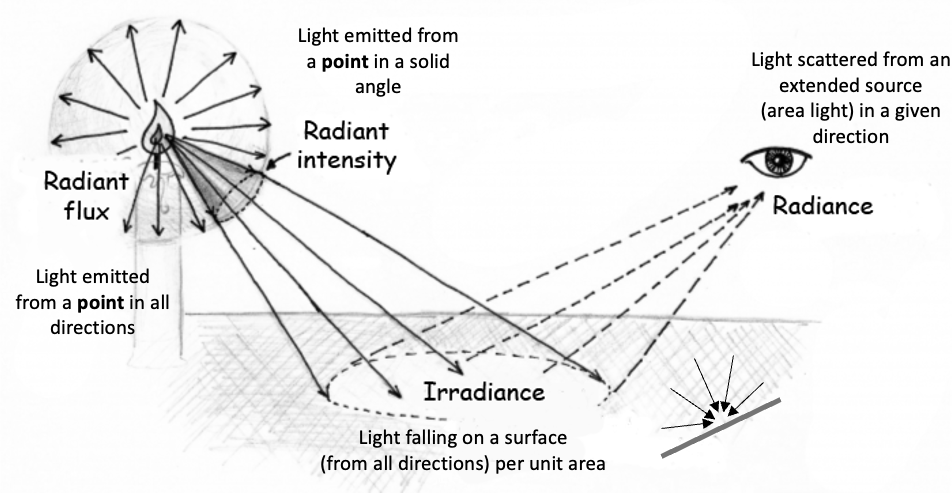
\includegraphics[width=1\textwidth,height=\textheight]{chapters/images/lightfields/02-measuring/01-radiometry.png}

}

\caption{\label{fig-radiometry}\textbf{The geometry of four radiometric
measures.}}

\end{figure}%

Figure~\ref{fig-radiometry} illustrates the geometry of four radiometric
measures. The upper left illustrates a point source. The \emph{radiant
flux} measures the total energy emitted from the point in all
directions. As for all radiometric measurements, the energy (watts) is
specified as a function of wavelength (watts/nm).

Often, we measure the light emitted by a point source in a particular
direction, the \emph{radiant intensity}. In that case we measure the
energy within a cone of rays in a particular direction. The standard
unit for angles in three-dimensions is the \emph{steradian}, just as the
radian is the standard unit for angles in two-dimensions. The radiant
intensity has units of watts per steradian per nanometer (watts/sr/nm).
Thus, if the measurement instrument measures energy over an angle of 0.5
steradians, we divide the measurement by 0.5. If the instrument sums
over 10 nm bands, we divide the energy by 10. In this way, the radiant
intensity normalizes the angle we measure to the unit steradian and per
nanometer. The standard symbol for radiant intensity is \(I(\lambda)\).

\begin{tcolorbox}[enhanced jigsaw, bottomtitle=1mm, titlerule=0mm, arc=.35mm, colbacktitle=quarto-callout-note-color!10!white, coltitle=black, toprule=.15mm, bottomrule=.15mm, breakable, colframe=quarto-callout-note-color-frame, left=2mm, opacityback=0, colback=white, title=\textcolor{quarto-callout-note-color}{\faInfo}\hspace{0.5em}{Steradians}, opacitybacktitle=0.6, toptitle=1mm, rightrule=.15mm, leftrule=.75mm]

\begin{figure}[H]

\centering{

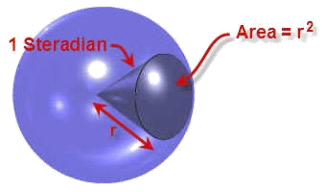
\includegraphics[width=0.4\textwidth,height=\textheight]{chapters/images/lightfields/02-measuring/01-radiometry-steradian.png}

}

\caption{\label{fig-steradian}Three-dimensional angle units are called
steradians. One steradian is defined as angle of the cone whose surface
area on a sphere of radius \(r\) is equal to \(r^2\). Because the
surface area of a sphere with radius \(r\) is \(4 \pi r^2\), it follows
that the complete sphere surrounding a point is \(4 \pi\) steradians.}

\end{figure}%

\end{tcolorbox}

\section{Radiance from a surface}\label{radiance-from-a-surface}

In many applications we measure radiance from a patch on an extended,
flat surface - such as a large light fixture with a diffuser, a wall, or
a large display screen. The geometry of such a measurement accounts for
two main factors illustrated in Figure~\ref{fig-foreshortening-sketch}.
First, we must account for the area of the surface patch, as seen from
the detector. For example, if the measured surface patch is a square
\(0.1\) meters on a side its area is \(A_s = (0.1~m)^2\). The area of
this patch, as seen from the detector, is foreshortened. We calculate
the foreshortened area using the angle between the viewing direction and
the surface normal, \(\theta\), which becomes
\(A_s \cos(\theta) ~ m^2\). Second, we account for the size of the
bundle of rays captured by the detector. We measure this size by its
three-dimensional angle, \(\omega ~ sr\), from a surface point that will
be measured by the detector. The \emph{radiance} combines the energy
measured at the sensor (\(watts/nm\)) with these geometric factors. The
standard symbol for spectral radiance is \(L(\lambda)\). It has units of
watts per nanometer per unit foreshortened-area per steradian:

\[ 
\frac{Watts}{nm ~ \cos(\theta) ~ m^2 ~ sr}
\]

\begin{figure}

\centering{

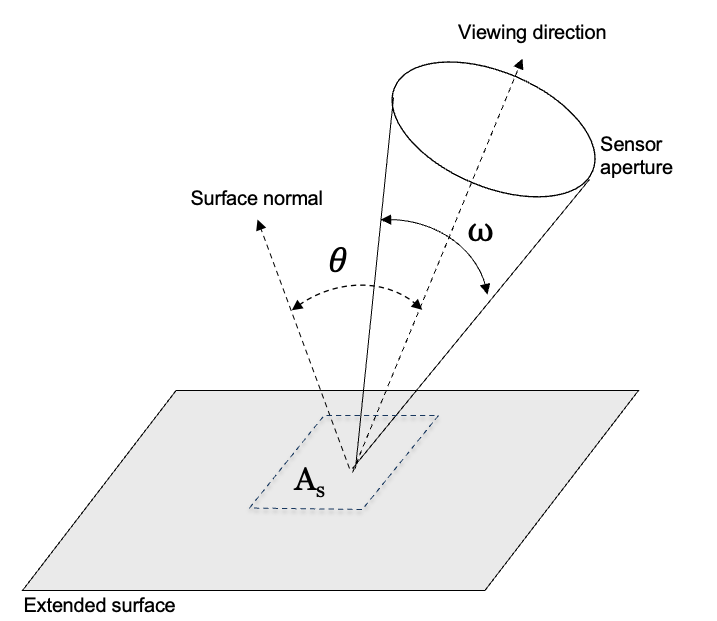
\includegraphics[width=0.6\textwidth,height=\textheight]{chapters/images/lightfields/02-measuring/01-foreshortening-sketch.png}

}

\caption{\label{fig-foreshortening-sketch}Geometric factors for
measuring radiance from an extended surface to a detector.}

\end{figure}%

\begin{tcolorbox}[enhanced jigsaw, bottomtitle=1mm, titlerule=0mm, arc=.35mm, colbacktitle=quarto-callout-note-color!10!white, coltitle=black, toprule=.15mm, bottomrule=.15mm, breakable, colframe=quarto-callout-note-color-frame, left=2mm, opacityback=0, colback=white, title=\textcolor{quarto-callout-note-color}{\faInfo}\hspace{0.5em}{Foreshortening}, opacitybacktitle=0.6, toptitle=1mm, rightrule=.15mm, leftrule=.75mm]

\begin{figure}[H]

\centering{

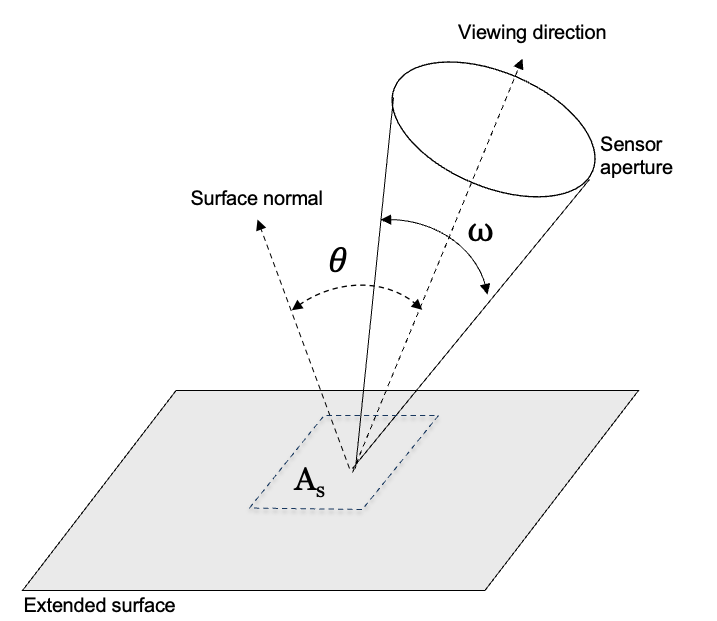
\includegraphics[width=0.8\textwidth,height=\textheight]{chapters/images/lightfields/02-measuring/01-foreshortening-sketch.png}

}

\caption{\label{fig-foreshortening}\textbf{Geometry and image size.} The
paper curves so that the circles are at different angles from the
camera. As the angle increases, the circles are smaller in the image
plane. You can judge the circle sizes; I suspect the physical difference
is greater your perceived size difference. (Maybe I make a set of rows
of circles on a cylinder. Then you ask which physical size on, say the
lowest rows, matches one of the full frontal circles.}

\end{figure}%

\end{tcolorbox}

\section{Irradiance}\label{irradiance}

Another important measurement is the radiance incident upon a surface,
the \emph{irradiance}. This quantity is important to calculate the
radiance available to an image sensor or the retina. It is also a
practical measure in assessing room lighting, say how much light will
arrive at a desk top. The irradiance sums the energy arriving from all
directions, hence no three-dimensional angles (steradians) are
specified. The irradiance measures the total energy per unit area of the
of the surface. The standard symbol for irradiance is \(E(\lambda)\),
has units \(watts/nm/m^2\).

\section{Radiometric units}\label{radiometric-units-1}

Figure~\ref{fig-radiometry-units} is a guide to help you remember the
four fundamental spectral radiometric measurements. Please note that
people will sometimes report a measure of any of these radiometric
quantities by summing the energy across all wavelengths. This would be
called, for example, the \emph{total radiance} or \emph{total
irradiance,} rather than the spectral radiance. I list the corresponding
\textbf{photometric} measurements in Chapter~\ref{sec-human}. The
photometric values are also a sum across wavelengths, but weighted by
the relative visual significance of the different wavelengths.

\begin{figure}

\centering{

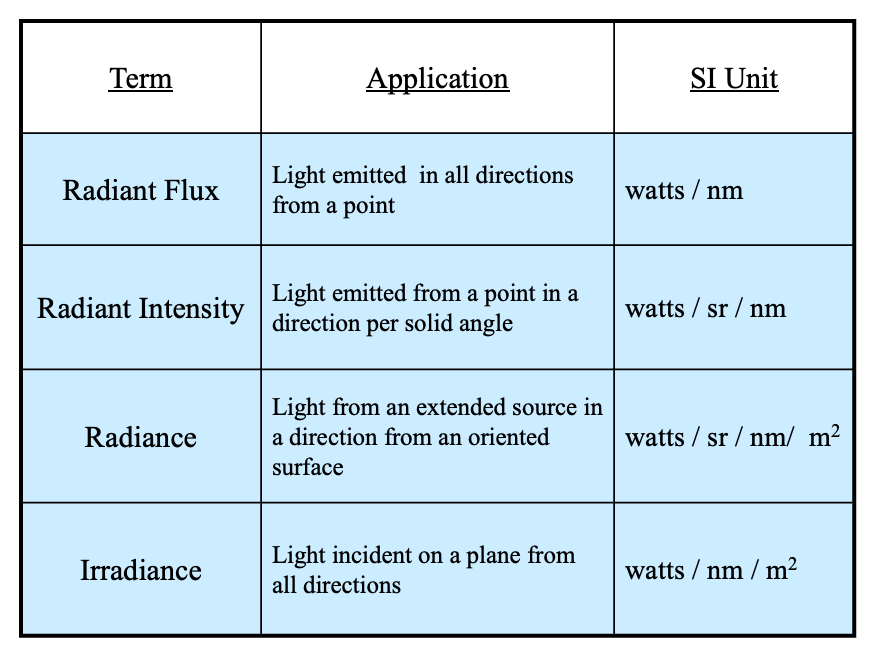
\includegraphics[width=1\textwidth,height=\textheight]{chapters/images/lightfields/02-measuring/01-radiometry-units.png}

}

\caption{\label{fig-radiometry-units}The four fundamental radiometric
measurement quantities. The table lists the name of the measurement, how
it is used, and the International System of Units (SI) definition for
each.}

\end{figure}%

\begin{tcolorbox}[enhanced jigsaw, bottomtitle=1mm, titlerule=0mm, arc=.35mm, colbacktitle=quarto-callout-note-color!10!white, coltitle=black, toprule=.15mm, bottomrule=.15mm, breakable, colframe=quarto-callout-note-color-frame, left=2mm, opacityback=0, colback=white, title=\textcolor{quarto-callout-note-color}{\faInfo}\hspace{0.5em}{Surface or point?}, opacitybacktitle=0.6, toptitle=1mm, rightrule=.15mm, leftrule=.75mm]

How do we determine whether we are measuring a part of a surface or a
point? The distinction between measuring a surface and a point source is
not always clear-cut. Here are some principles, though none is
definitive.

\begin{itemize}
\tightlist
\item
  \textbf{Distance:} If the distance to the source is significantly
  larger than the dimensions of the source itself, it can be
  approximated as a point source.
\item
  \textbf{Solid Angle:} If the solid angle subtended by the source at
  the detector is very small, it can be approximated as a point source.
\item
  \textbf{Precision:} If high accuracy is required, it's generally
  better to use the radiance formula, even for small surfaces. This
  allows you to account for the angular distribution of the emitted
  radiation. If lower accuracy is sufficient, and the source can be
  reasonably approximated as a point source, the radiant intensity
  formula can be used.
\end{itemize}

These recommendations are filled with imprecision that I always try to
remove. They contain words, like `small', `large', `high', and `low'
because there is no fixed threshold at which a surface definitively
becomes a point source. It is your decision whether to treat the source
as a point. What is important is to tell people exactly what you did. If
they don't like your choice, they can do it their own way. Or they can
ask you - nicely - to try it another way.

\end{tcolorbox}

After considering the four fundamental radiometric measurements
presented here, it might occur to you that there is additional
information we could represent. For example, it would be possible to
measure the radiance of a patch of an extended surface at many different
viewing angles. This would produce a function whose value depends on the
two parameters, azimuth (\(\alpha\)) and elevation (\(\beta\)) that
define the viewing angle. Similarly, we might decide to measure the
irradiance as a function of these two incident angles. We will return to
these more advanced specifications when we introduce the bidirection
reflectance distribution function in Section~\ref{sec-properties-brdf}.

\chapter{Light field properties}\label{sec-lightfield-properties}

\section{Light field properties
overview}\label{sec-lightfield-properties-overview}

Many image systems are engineered to quantify scene properties, such as
an object's size, its distance to the sensor, or its material. These
measurement-oriented systems have many applications, including
industrial quality control, autonomous navigation, and medical
diagnostics. Even in consumer photography, where the primary goal is
often to capture and render a visually compelling representation of a
scene, estimating underlying physical characteristics --- like the
ambient illumination --- can significantly enhance performance. As
highlighted in the Preface with the quote from Helmholtz
Figure~\ref{fig-helmoltz}, inferring scene properties is arguably the
fundamental task of visual perception.

A common challenge in many image system applications is that the
measurement process is often underdetermined. This means that multiple
distinct scene properties could potentially lead to the same observed
measurement. In such situations, a powerful principle, often attributed
to Thomas Bayes, becomes invaluable. Bayes' Rule suggests that when
faced with multiple plausible solutions, we should select the one that
is most probable. While the general principle is conceptually elegant,
the practical challenge lies in accurately determining the likelihood of
each potential solution.

While we may not always possess explicit knowledge about the
probabilities of different solutions, we can often leverage prior
information or learn from experience. One effective strategy for making
more informed inferences is to understand the inherent regularities
present in the world. In this section, we will explore some fundamental
regularities concerning the spectral (wavelength-dependent) and spatial
characteristics of natural images.

Identifying and leveraging regularities within scene radiance is a
central theme we will revisit throughout this book In specific,
well-defined applications, such as medical imaging or controlled
industrial inspection environments, these regularities can significantly
constrain the set of plausible interpretations, providing a valuable and
precise guide for analysis.

\section{Representing regularities}\label{representing-regularities}

When considering the scene regularities, we face two interconnected
challenges. First, how do we come to understand these underlying
patterns? In some instances, our knowledge stems from building physical
models of the signals, where regularities emerge as a natural
consequence of our understanding. The solar radiation analysis below
provides a good example of this. In other cases, we learn about
regularities through empirical observation of numerous examples,
employing computational tools to quantify these patterns. Our
discussions on surface reflectances and the characteristic spatial
structure of natural images will illustrate this approach.

Two classical mathematical frameworks are fundamental for specifying
regularities across various scientific and engineering disciplines, and
both will feature prominently in this book. Bayes' Rule offers a
powerful yet straightforward way to reason about probabilities. More
generally, probability distributions provide a versatile language for
representing the likelihood of observations. While these distributions
can sometimes be directly used in simulations, their incorporation can
often present significant computational hurdles.

A second widely employed mathematical tool is dimensionality reduction,
particularly techniques based on linear models. Dimensionality reduction
offers a highly practical computational approach for simplifying complex
datasets. However, it often provides only an approximate representation
of the underlying statistical regularities.

More recently, neural network training has emerged as a potent method
for inferring statistical regularities from large datasets,
simultaneously yielding a computationally tractable model. This
data-driven approach is proving increasingly valuable across numerous
applications.

In this section, we will delve into the two classical techniques. They
remain indispensable tools, often providing crucial insights into the
physical principles governing the system. We will then apply them to key
descriptions of scene spectral radiance. As we progress through
subsequent sections of the book, we will explore how neural network
training is increasingly being integrated into image systems
engineering.

\subsection{Bayes Rules}\label{bayes-rules}

If we wish to know the probability of a specific condition, \(C\), being
true given measured data,~\(d\), we can use the laws of probability to
write

\[
P(C | d) = \frac{P(d \cap C)}{P(d)} = \frac{P(d \cap C) P(C)}{P(d) P(C)}= \frac{P(d | C) P(C)}{P(d)}
\]

\begin{tcolorbox}[enhanced jigsaw, colframe=quarto-callout-note-color-frame, left=2mm, opacityback=0, colback=white, arc=.35mm, toprule=.15mm, rightrule=.15mm, leftrule=.75mm, bottomrule=.15mm, breakable]
\begin{minipage}[t]{5.5mm}
\textcolor{quarto-callout-note-color}{\faInfo}
\end{minipage}%
\begin{minipage}[t]{\textwidth - 5.5mm}

\vspace{-3mm}\textbf{The terms in Bayes' Rule}\vspace{3mm}

\begin{itemize}
\tightlist
\item
  \(P(C | d)\) - \textbf{posterior probability} of C given d.
\item
  \(P(d|C)\) - \textbf{likelihood} of d given C.
\item
  \(P(C)\) - \textbf{prior probability} of C.
\item
  \(P(d)\) - \textbf{marginal likelihood} of d.
\end{itemize}

\end{minipage}%
\end{tcolorbox}

Implementing Bayes' Rule through this formula requires knowing the
likelihood of the data given the condition, \(P(d|C)\). This knowledge
can come from a model of the process that enables us to simulate the
data. Being able to work out this probability is a fundamental task for
the scientist or engineer. A more difficult challenge in using Bayes'
Rule is that we often have little idea about the prior, \(P(C)\). The
cases in which we do have this world knowledge can be very valuable.

There are many cases, often in the applied sciences and engineering,
when enough is known to apply Bayes' Rule. A good example is a medical
image diagnostic, say the chance of having a dark spot on of contrast
\(d\) on the lung to detect a cancerous lesion. We may have measurements
from many people, and in retrospect they either will have the disease or
not. We can use these data to estimate the likelihood of \(P(d \mid C)\)
and \(P(d \mid \neg C)\). We may further have historical data of the
percentage of people in the population who have the disease, \(P(C)\).
The marginal probability is

\[
P(d) = P(d \mid C) P(C) + P(d \mid \neg C) P(\neg C)
\]

From these terms, we can compute the probability of having the posterior
probability, \$P(C \mid d)\$. There are many cases in which we do not
have the data to estimate all of the needed likelihoods. In those cases,
we can use other tools.

\subsection{Linear models}\label{sec-linear-models}

Linear models have many uses in science and engineering. One application
is representing certain regularities in the data. Specifically, suppose
we have a collection of measurement vectors, each with \(D\) values. We
can express each of the vectors as the weighted sum of a set of \(M\)
vectors, which we call the \emph{basis} vectors. If \(M\) is much
smaller than \(D\), the basis set captures a regularity that is present
in the original data set.

As an example, suppose the data are a set of radiance spectra,
\(d(\lambda)\), we measured over the visible range from 380 nm to 780 nm
in 1 nm steps; hence, each vector, \(d\), has 401 values. After making a
few thousand (or million) measurements, we discover that we can closely
approximate any of the measurements, \(d_j\), as the weighted sum of
\(M\) basis functions, \(B_i\). We write the approximation this way:

\begin{equation}\phantomsection\label{eq-linear1}{
d_j(\lambda) \approx \sum_{i=1}^{M} B_i(\lambda) w_{ij}
}\end{equation}

There are a many tools to find basis vectors, \(\mathbf{B_i}\), and
these tools rely on different objectives. Sometimes, the basis vectors
are selected from physical or computational principles. This is the case
for the Fourier basis functions, which are the harmonic functions, and
are a natural part of magnetic resonance imaging, sound, and heat
transfer. It is also common to select \(M\) basis functions that explain
the most variance in the data, which is the choice we make when using
Principal Components Analysis (PCA) that relies on the important matrix
decomposition the singular value decomposition (SVD).

In both of these cases, Fourier and PCA, the basis vectors are
orthogonal, which means that the inner product\footnote{Widely used
  synonyms for the term inner product are \emph{dot product} and
  \emph{scalar product}.} of any pair of basis vectors is zero. The
mathematical expression for the inner product and orthogonality is

\[
0 = \sum_{\lambda} B_i(\lambda) B_j(\lambda)
\]

It is quite common to use matrix notation to express the linear model.
With this notation, the linear model places the basis vectors into the
columns of a matrix, \(\mathbf{B}\). Each data vector, \(\mathbf{d_j}\),
is the product of a weight vector, \(\mathbf{w_j}\) times the matrix of
basis vectors.

\begin{equation}\phantomsection\label{eq-linearmatrix}{
\mathbf{d_j} = \mathbf{B} \mathbf{w_j}
}\end{equation}

This regularity is often called dimension-reduction. It is a helpful
regularity, but quite different from knowing the full probability
distribution. The regularity allows us to take the high dimensional
data, say with 401-vectors, and represent them with many fewer numbers,
say the 10 or 20 weights. In that sense, the reduction informs us about
the likelihood of certain data sets. But there remains a much more that
can be learned about the data because not all of the different weights
are likely, or in some cases physically realizable. Thus, the
dimensionality gets you part of the way there, but studying the
properties of thew weights can provide even more information (DiCarlo
and Wandell (2003))

Linear models appear in many places in this book, with many different
applications. If you would like to read more about them, have a look at
the chatty discussion in Appendix \textbf{?@sec-linearmodels}. From
there you can find your way to more advanced and authoritative
literature. The Appendix also contains pointers to important nonlinear
methods that - in some circumstances - can be very helpful (Maaten et
al. (2008)).

In the following sections I describe regularities that have been
discovered about various spectral measures. We begin with regularities
concerning the spectral properties in the visible band. We then turn to
regularities concerning the spatial properties of natural images, again
in the visible band.

\chapter{Spectral regularities}\label{sec-spectral-regularities}

\section{Spectral regularities
overview}\label{sec-spectral-regularities-overview}

\section{Solar Radiation}\label{solar-radiation}

The Sun serves as Earth's primary radiation source. The radiation
emitted from the Sun's surface in the visible spectrum remains
relatively consistent over time. Due to its significance for imaging and
human vision, skylight became an early subject of scientific
investigation.

In 1814, Joseph Fraunhofer observed and carefully documented numerous
dark lines in the solar spectrum, now known as \textbf{Fraunhofer lines}
It was subsequently discovered that these lines are present because
light generated in the Sun's hot, dense interior (photosphere) travels
through its cooler outer layers (chromosphere and corona). During this
passage, atoms and ions absorb specific wavelengths of light that
correspond precisely to their electron transitions. The reliability of
these solar absorption lines allows scientists to use them as reference
points to calibrate laboratory instruments for spectral measurements.
For example, James Clerk Maxwell used these lines to calibrate the first
experimental rig for human color-matching (Maxwell (1860),Maxwell and
Zaidi (1993)).

\begin{figure}

\centering{

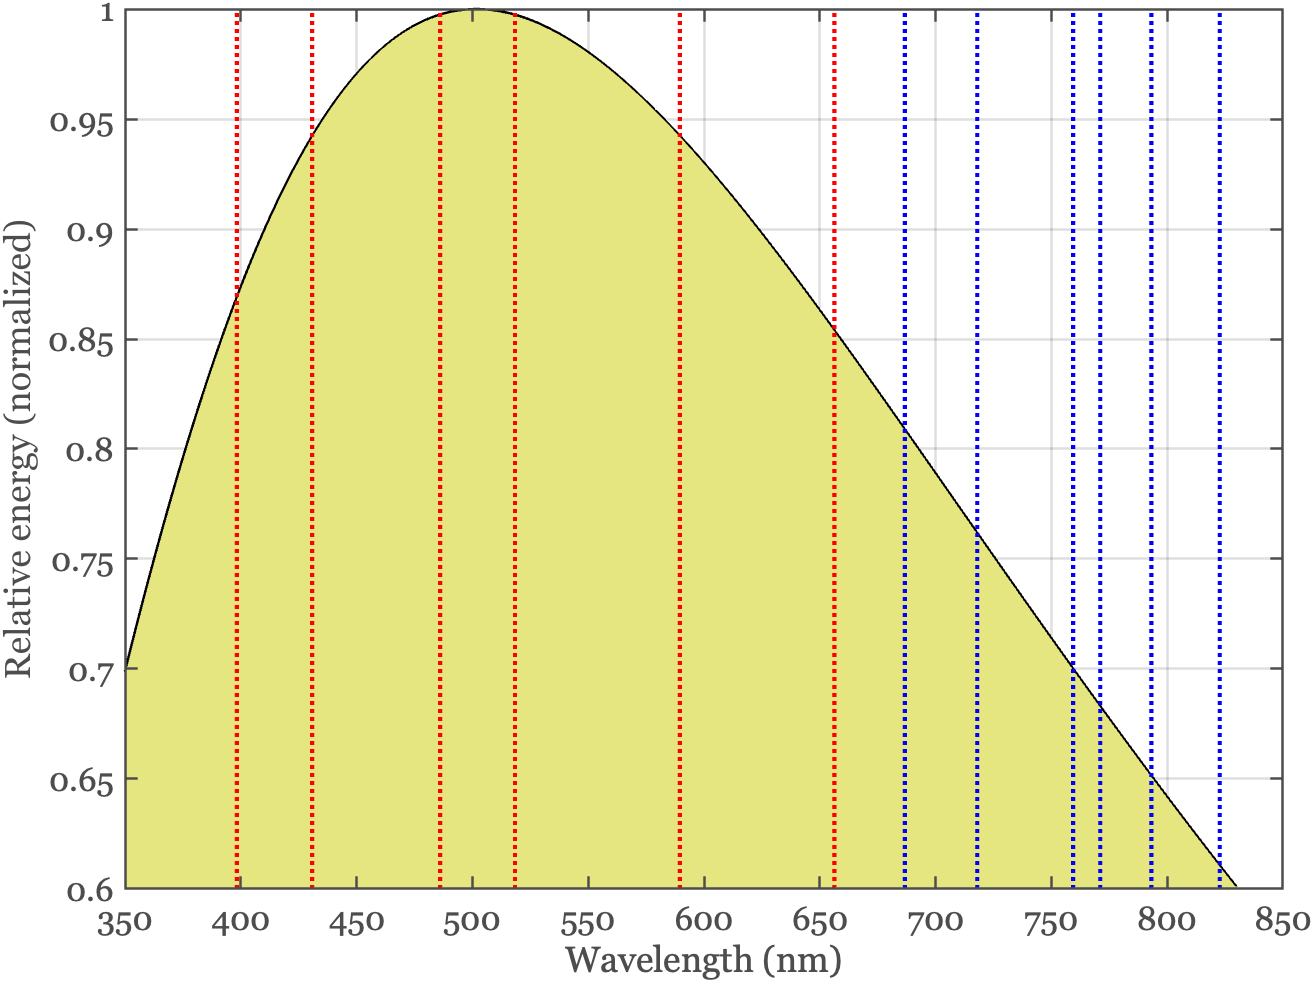
\includegraphics[width=0.6\textwidth,height=\textheight]{chapters/images/lightfields/04-spectral/01-solar-lines.png}

}

\caption{\label{fig-solarspectrum}The black curve displays the relative
solar spectrum, which is stable over time. The red lines indicate are
drawn at wavelengths where the spectrum exhibits narrow intensity
reductions, known as Fraunhofer lines, that originate from ions and
atoms in the Sun's outer layers. The blue dotted lines mark intensity
reductions caused by atmospheric water vapor.}

\end{figure}%

\begin{tcolorbox}[enhanced jigsaw, colframe=quarto-callout-note-color-frame, left=2mm, opacityback=0, colback=white, arc=.35mm, toprule=.15mm, rightrule=.15mm, leftrule=.75mm, bottomrule=.15mm, breakable]
\begin{minipage}[t]{5.5mm}
\textcolor{quarto-callout-note-color}{\faInfo}
\end{minipage}%
\begin{minipage}[t]{\textwidth - 5.5mm}

\vspace{-3mm}\textbf{\phantomsection\label{sec-fraunhofer}\href{https://en.wikipedia.org/wiki/Joseph_von_Fraunhofer}{Joseph
Fraunhofer (1787-1826)}}\vspace{3mm}

Fraunhofer was a brilliant applied researcher who worked on the physical
properties of materials, particularly glass. He also made important
contributions to the theory of image formation and optics.

The Fraunhofer lines, which he discovered while building a device to
measure the spectral transmissivity of glass, are reported in a paper
reviewing the properties of glass. These relative intensity of these
lines are determined by the material composition of the stars, and these
measurements are stilled used in astronomy to determine the composition
of celestial bodies. Fraunhofer died at the age of 39, poisoned by heavy
metal vapors used in his material research. Europe's largest body for
the advancement of applied research, the Fraunhofer Society, is named to
honor him.

\begin{figure}[H]

{\centering 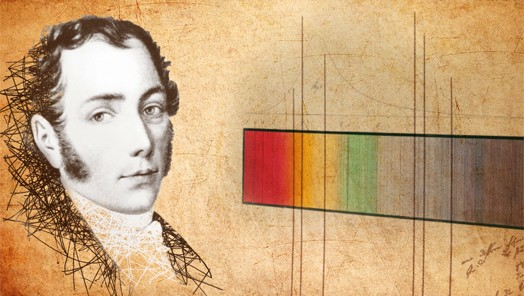
\includegraphics[width=4.07292in,height=\textheight]{chapters/images/people/Fraunhofer.png}

}

\caption{Joseph Fraunhofer.}

\end{figure}%

This is a good historical review of the
\href{https://joachimweise.github.io/post/2020-10-20-fraunhofer-lines/}{Fraunhofer
lines} and subsequent work.

\end{minipage}%
\end{tcolorbox}

\section{Atmospheric Effects}\label{atmospheric-effects}

Some of the spectral absorption lines observed at Earth's surface
originate from a different source: water vapor (H₂O) and other molecules
in Earth's atmosphere. Unlike the stable solar absorption lines, these
atmospheric absorptions fluctuate relatively quickly with changing
weather conditions. There is also atmospheric variation in the skylight
spectral power with the time of day, as the radiation's path length
through the atmosphere varies. Longer path lengths --- such as during
sunrise or sunset --- modify the spectral composition of radiation
reaching Earth's surface.

A number of different groups have reported measurements of solar
radiation at the Earth's surface at varying times of day and weather
conditions (Judd et al. 1964). Figure \#fig-daylights shows examples of
typical variation in the shape of the spectral power distribution in
Granada, Spain (Hernández-Andrés et al. 2001) and Stanford, California
(DiCarlo and Wandell 2000).

\begin{figure}

\centering{

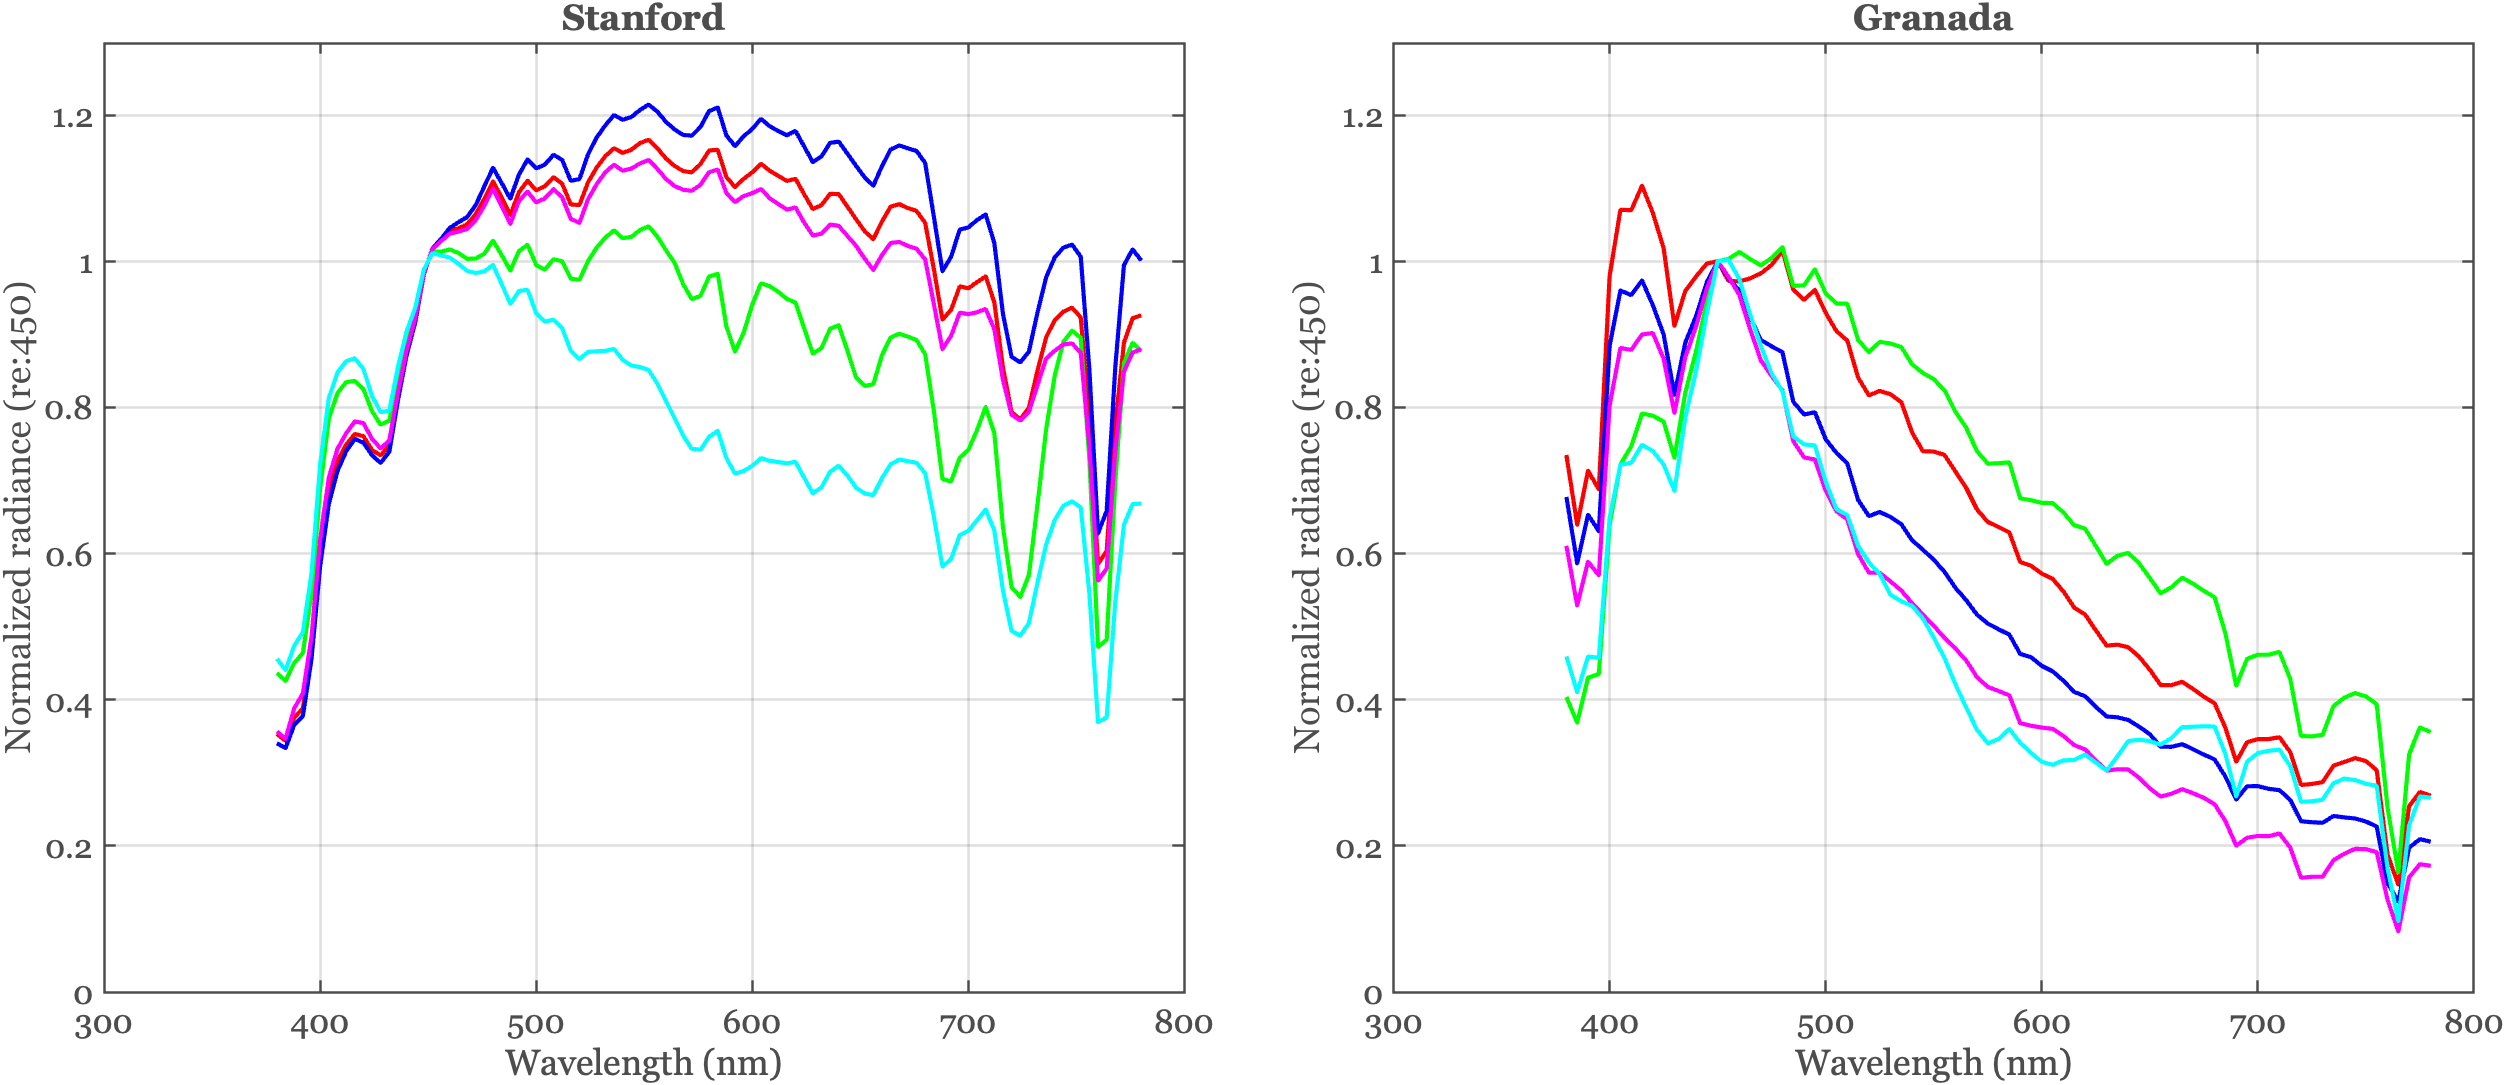
\includegraphics[width=0.9\textwidth,height=\textheight]{chapters/images/lightfields/04-spectral/01-solar-samples.png}

}

\caption{\label{fig-daylights}The spectral power distribution of
daylights sampled at the Earth's surface in Granada, Spain (left) and
Stanford, California (right) at different times of day and weather
conditions. The spectra have been scaled to be equal at 450 nm. The
curves have different slopes, and their shapes vary with weather and
time-of-day. Identifiable Fraunhofer lines and water vapor lines are
present in the measurements.}

\end{figure}%

These combined factors---atmospheric composition and path length
variations---create a complex, but restricted, distribution of sky
radiances at the Earth's surface. To summarize the regularities,
scientists and engineers have created linear models that can represent
the natural variations. The original model was introduced by Judd,
Macadam and Wyszecki (Judd et al. 1964). They analyzed skylight at the
Earth's surface using about 650 different measurements. They found that
the spectral power distributions, normalized to remove absolute radiance
level, could be modeled as the weighted sum of three terms: a mean and
two basis functions (Figure Figure~\ref{fig-ciedaylight}). Such a model
is useful because it enables us to represent any particular sample using
just three numbers, the two weights and an overall scalar to match the
level. The model is also useful for applications in which a scene is
acquired under full sky illumination, and we would like to estimate the
spectral power distribution of the skylight. We only need to estimate
the weights, and from those we can make a good estimate of the full
spectrum.

\begin{figure}

\centering{

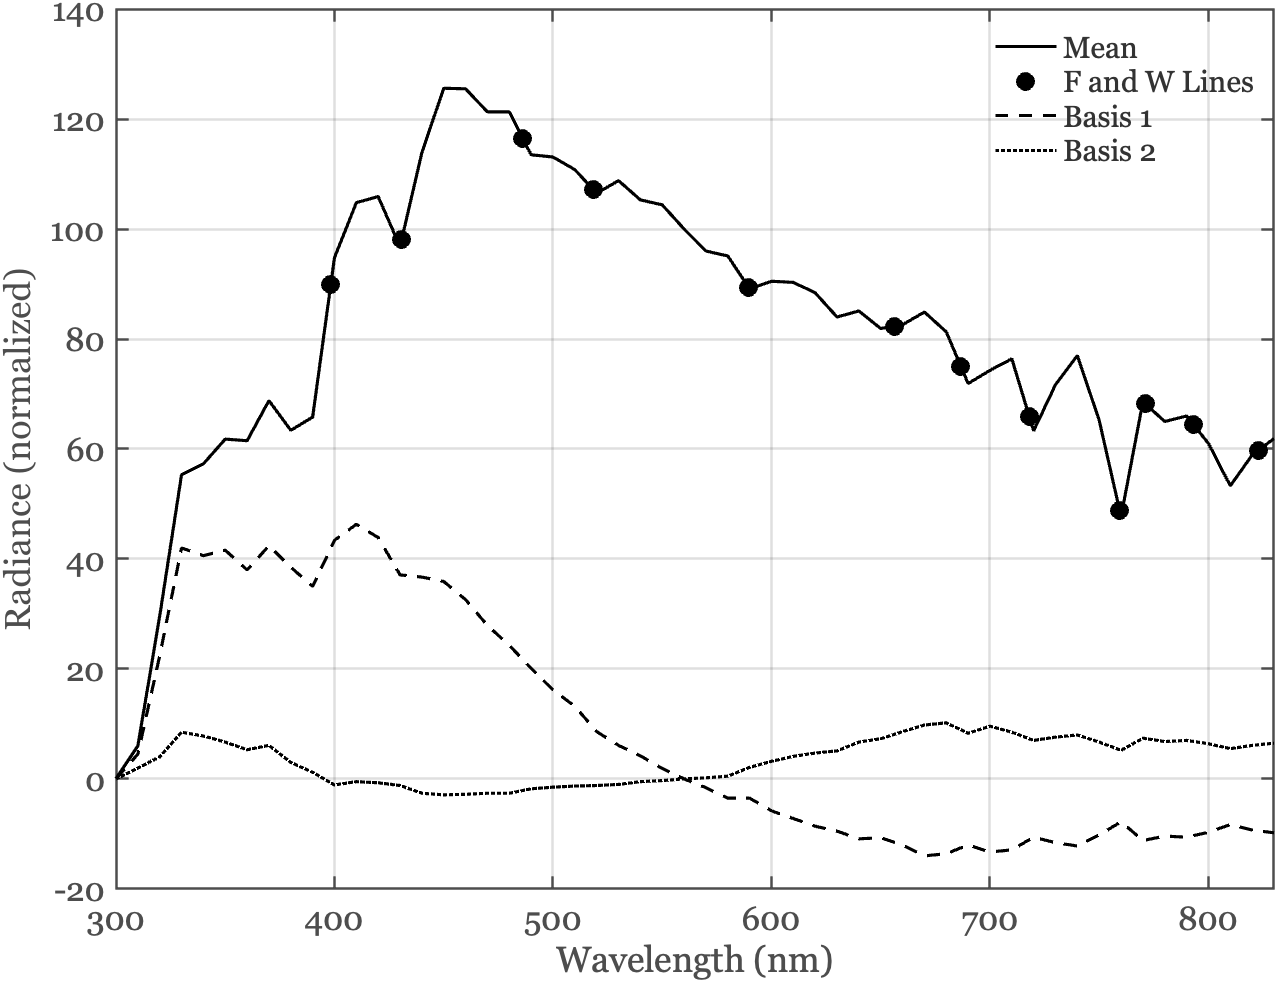
\includegraphics[width=0.5\textwidth,height=\textheight]{chapters/images/lightfields/04-spectral/01-solar-basis.png}

}

\caption{\label{fig-ciedaylight}The solid curve shows the mean daylight
spectrum measured by Judd, Macadam and Wyszecki Judd et al. (1964).
Their measurements evolved into a CIE standard linear model for
daylights. The solid circles are placed at the wavelengths of Fraunhofer
and atmospheric water vapor lines. The dotted and dashed curves are
basis functions. Together with the mean, they form a linear model of
daylight spectral power distributions.}

\end{figure}%

\begin{tcolorbox}[enhanced jigsaw, colframe=quarto-callout-note-color-frame, left=2mm, opacityback=0, colback=white, arc=.35mm, toprule=.15mm, rightrule=.15mm, leftrule=.75mm, bottomrule=.15mm, breakable]
\begin{minipage}[t]{5.5mm}
\textcolor{quarto-callout-note-color}{\faInfo}
\end{minipage}%
\begin{minipage}[t]{\textwidth - 5.5mm}

\vspace{-3mm}\textbf{Do it yourself daylight spectra}\vspace{3mm}

When he was a student at Stanford, Jeff DiCarlo decided to measure the
daylight outside his office for himself (DiCarlo and Wandell 2000).
Checking things for himself is in his nature. Jeff pointed a spectral
radiometer at a calibrated surface outside his window and configured a
computer to make about ten thousand measurements, one a minute, during
the course of a few rainy weeks in California (January 28, 2000 to
February 16, 2000). I included a sample of 1000 of these measurements in
ISETCam, and I have the whole group along with time stamps if you want
them.

\begin{figure}[H]

\centering{

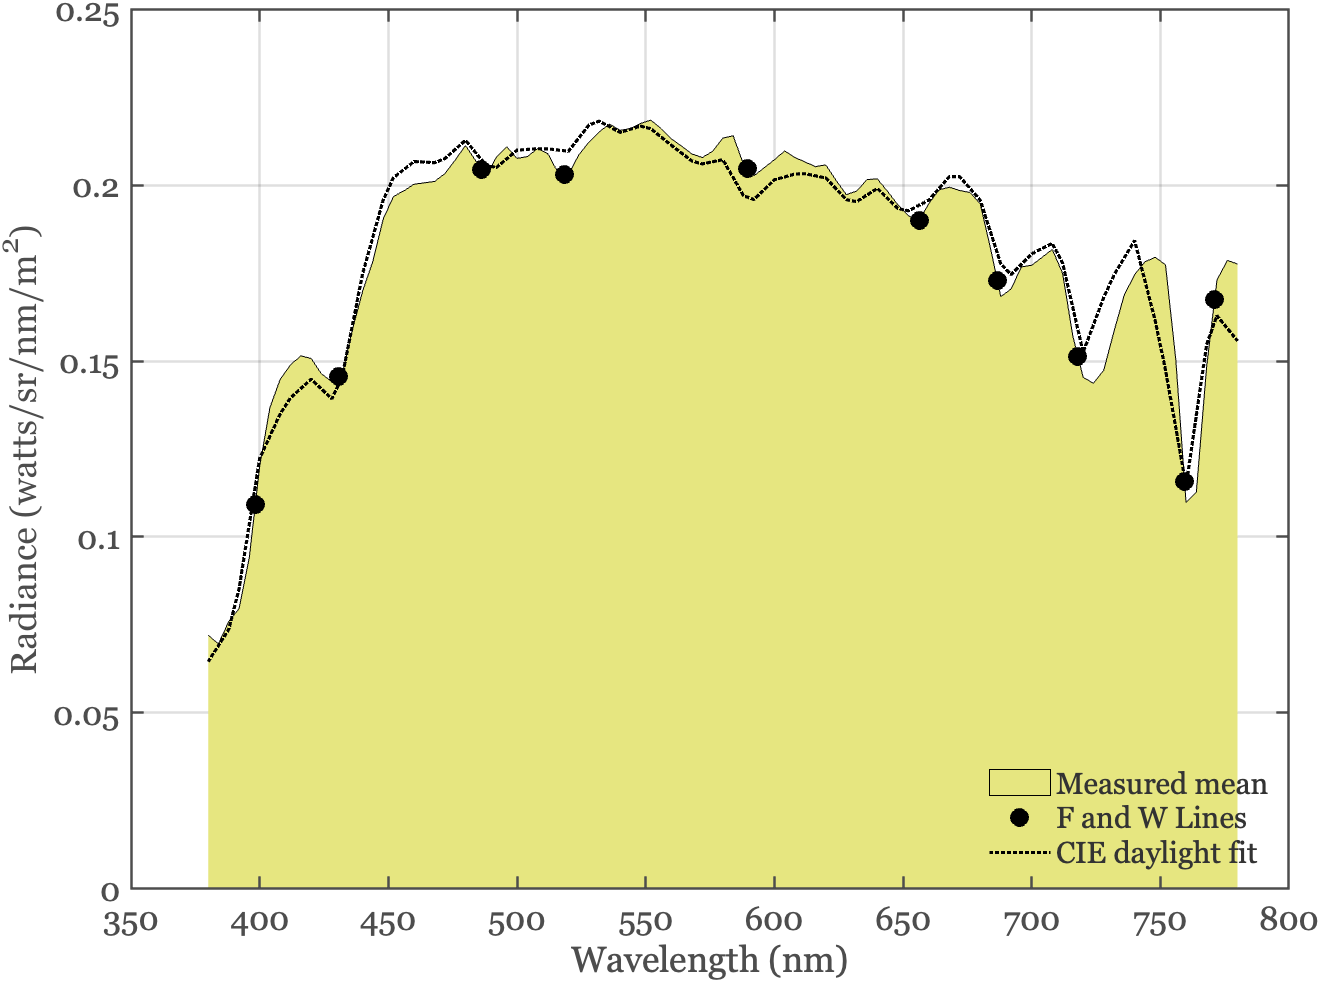
\includegraphics[width=0.5\textwidth,height=\textheight]{chapters/images/lightfields/04-spectral/01-solar-stanford.png}

}

\caption{\label{fig-stanfordsun}Average daylight measurements on the
Stanford campus (solid) and CIE daylight basis fit to the measured
average (dotted). The solid circles are placed at the locations of
Fraunhofer and water vapor wavelengths.}

\end{figure}%

Figure~\ref{fig-stanfordsun} shows the mean spectral power distribution
of these measurements. You can see that the instrument recorded several
`notches' the spectrum at wavelengths corresponding to the Fraunhofer
and water vapor lines. We also asked whether these data could be fit by
the CIE linear model - and the least-squares fit is shown by the dotted
line. I suspect there is an instrument calibration error of a few
nanometers at wavelengths above 700nm, and were I to write a research
paper based on these data, I would probably introduce the correction
because I believe the physics on the locations of these wavelengths is
secure. This analysis might provide you with a sense of the relative
accuracy of measuring and approximating spectra with conventional lab
equipment.

\end{minipage}%
\end{tcolorbox}

The regularities in the sky radiance are even more constrained than the
linear model. First, the weights are correlated: When you know one of
the weights, you can make a reasonable guess about the other weight.
Also, some weights are impossible because they would produce negative
values in the spectrum DiCarlo and Wandell (2000). Thus, the linear
model gets us part of the way to establishing the regularities, but
there is even more to be measured.

\begin{tcolorbox}[enhanced jigsaw, colframe=quarto-callout-note-color-frame, left=2mm, opacityback=0, colback=white, arc=.35mm, toprule=.15mm, rightrule=.15mm, leftrule=.75mm, bottomrule=.15mm, breakable]
\begin{minipage}[t]{5.5mm}
\textcolor{quarto-callout-note-color}{\faInfo}
\end{minipage}%
\begin{minipage}[t]{\textwidth - 5.5mm}

\vspace{-3mm}\textbf{Daylight weights}\vspace{3mm}

\subsection{Correlated weights}\label{correlated-weights}

\begin{figure}[H]

\centering{

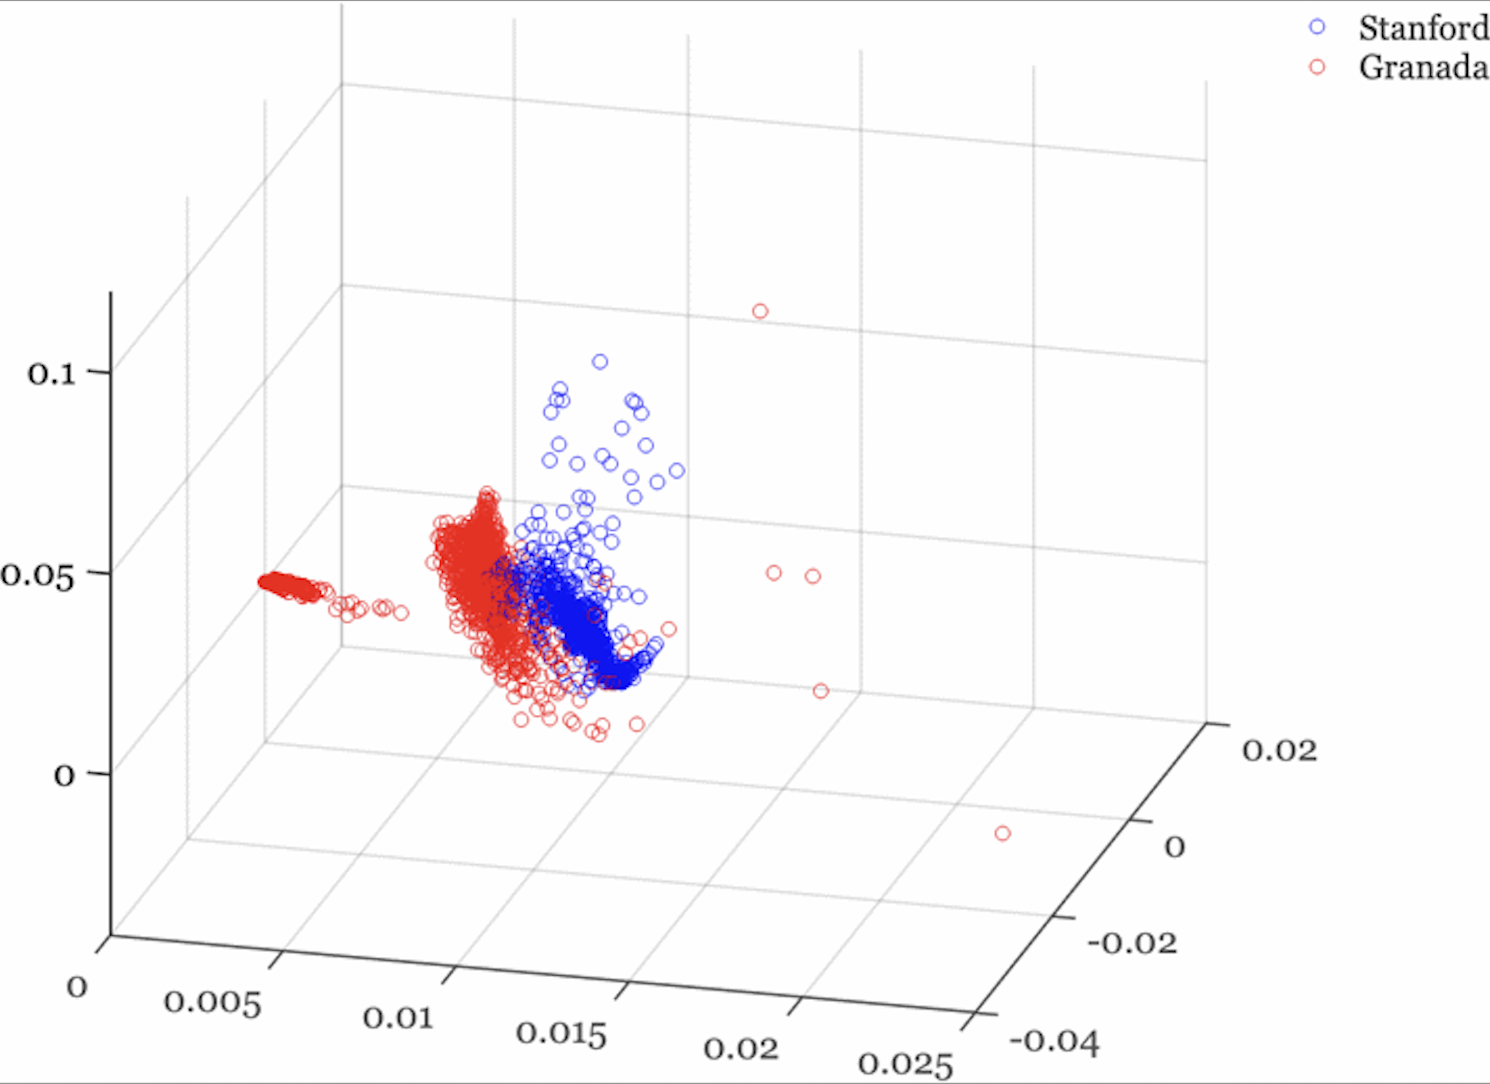
\includegraphics[width=3.875in,height=\textheight]{chapters/images/lightfields/04-spectral/01-dayweights3d-still.png}

}

\caption{\label{fig-dayweights}(PDF Snapshot): The daylight basis
weights from the Granada and Stanford data sets. The weights are
clustered within a plane, although there are occasional outliers. The
orthogonality of the basis functions does not imply independence or
orthogonality of the measured basis weights.}

\end{figure}%

\end{minipage}%
\end{tcolorbox}

\section{Surface spectral reflectance
regularities}\label{surface-spectral-reflectance-regularities}

Vision enables us to interpret the environment by recording the how the
ambient illumination interacts with things (e.g., objects) and stuff
(e.g., water). Four things can happen when electromagnetic radiation
interacts with a surface. The radiation arriving at a surface might be
(a) reflected, (b) absorbed, (c) pass through, or (d) interact with the
material and generate new radiation (fluorescence). We will consider
each of these interactions in different sections of this book. Here, we
describe some regularities how light is reflected from many common
materials.

\begin{tcolorbox}[enhanced jigsaw, colframe=quarto-callout-note-color-frame, left=2mm, opacityback=0, colback=white, arc=.35mm, toprule=.15mm, rightrule=.15mm, leftrule=.75mm, bottomrule=.15mm, breakable]
\begin{minipage}[t]{5.5mm}
\textcolor{quarto-callout-note-color}{\faInfo}
\end{minipage}%
\begin{minipage}[t]{\textwidth - 5.5mm}

\vspace{-3mm}\textbf{Things and Stuff}\vspace{3mm}

I am fond of a distinction that Ted Adelson introduced to help think
about the environment: \emph{things and stuff}'' Adelson (2001). Things
are the countable, discrete objects with defined shapes and boundaries
(e.g., cars, chairs, animals). Stuff is amorphous materials or textures
without fixed boundaries (e.g., water, grass, sky, sand). Dividing the
environment into these categories also helps us set computational goals.

\begin{figure}[H]

\centering{

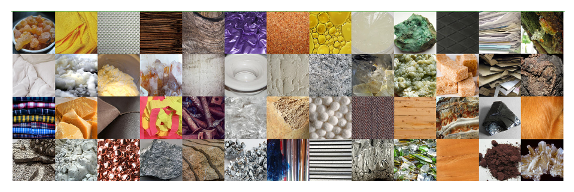
\includegraphics[width=0.7\textwidth,height=\textheight]{chapters/images/lightfields/04-spectral/01-things-stuff.png}

}

\caption{\label{fig-things-stuff}The distinction between \emph{things}
and \emph{stuff} plays a role in vision science and now computer vision.
These images, from Schmidt et al. (2025), illustrate what is meant by
stuff. The authors explored the appearance of materials and stuff, in
contrast to much other work aimed at identifying things.}

\end{figure}%

The distinction helps separate out the types of algorithms we might
apply to understand the environment. Segmentation applies to
\emph{things} which are analyzed for object identity and function; in
contrast, \emph{stuff} is regionally based on texture and material
properties. A great deal of computer vision focuses on tasks such as
naming or counting cars on the road, people in the room, airplanes in
the sky. We wish to be able to recognize such things whatever their
material might be. A vision system must also be able to make judgments
about a sandy beach, a cloudy sky, a grassy hillside. We wish to be able
to recognize such stuff whatever its shape might be.

A related challenge in human vision is quantifying the appearance of
things and stuff, and for this challenge surface reflectance, texture,
and context (e.g., ambient illumination, or what things and stuff are
nearby) all play a role Schmid et al. (2023). A corresponding concept -
something we might call appearance for a computer vision system - seems
desirable. One way to formulate the problem of appearance for a computer
vision system is to use and estimate of material reflectance and texture
to mean appearance for the computer.

\href{https://datasetninja.com/cocostuff164k}{The COCO-Stuff 164k
dataset} has many images categorized in terms of `things' and stuff.

\end{minipage}%
\end{tcolorbox}

The radiation incident on a small, planar patch of material can come
from different directions, which we can specify by two angles. The
intensity of the reflected radiation will also vary with direction (two
more dimensions). The incident and reflected light can be measured as
the intensity for different wavelengths and polarizations (two more
dimensions). We will set aside fluorescence for the present, returning
to it later. Hence, a full description of surface spectral reflectance
requires specifying multiple parameters.

Despite this potential complexity, there are many relatively simple
cases that are simpler to describe and still useful. We will work our
way up from the simplest case to increasingly complex descriptions,
identifying regularities along the way.

\section{Diffuse reflectance}\label{diffuse-reflectance}

An important type of reflectance, \emph{diffuse reflectance}, or
\emph{Lambertian reflectance}. The incident light is reflected with
roughly equal intensity in all directions within the hemisphere above
the surface. This occurs when the surface is rough at a microscopic
level, comprising many little facets. When the incident light arrives,
it will be reflected by one of the facets which are oriented equally in
all different directions. Importantly, not all of the incident light is
scattered; some of it is absorbed. The fraction that is absorbed varies
with wavelength. The fraction that is scattered is called the diffuse
spectral reflectance function.

Many objects, like paper, clothing, and walls, are mainly diffuse
reflectors, and the spectral reflectance function is a dominant factor
in how we perceive surface color. You can judge to what extent a
material is a diffuse reflectance by viewing it from different
positions, say by moving your head or walking around the room. For
diffuse materials the reflected light will be about the same. Other
materials, such as the highlights reflected from a car, vary in
intensity and color appearance as you move around, appearing bright from
some positions but not others. Such materials are not diffuse.

\begin{tcolorbox}[enhanced jigsaw, colframe=quarto-callout-note-color-frame, left=2mm, opacityback=0, colback=white, arc=.35mm, toprule=.15mm, rightrule=.15mm, leftrule=.75mm, bottomrule=.15mm, breakable]
\begin{minipage}[t]{5.5mm}
\textcolor{quarto-callout-note-color}{\faInfo}
\end{minipage}%
\begin{minipage}[t]{\textwidth - 5.5mm}

\vspace{-3mm}\textbf{Johan Lambert}\vspace{3mm}

The term Lambertian surface honors the Swiss physicist,
\href{https://en.wikipedia.org/wiki/Johann_Heinrich_Lambert}{Johann
Lambert} (1728-1777) who formalized the mathematical description. Many
surfaces are modeled as Lambertian in computer graphics, or assumed to
be Lambertian in computer vision estimates of the environment. Examples
of materials with Lambertian reflectance include chalk, plaster,
uncoated paper, matte paints made from pigments.

Adding additional details about the surface reflectance can improve the
system performance, but it is common to start with a Lambertian
approximation.

\begin{figure}[H]

\centering{

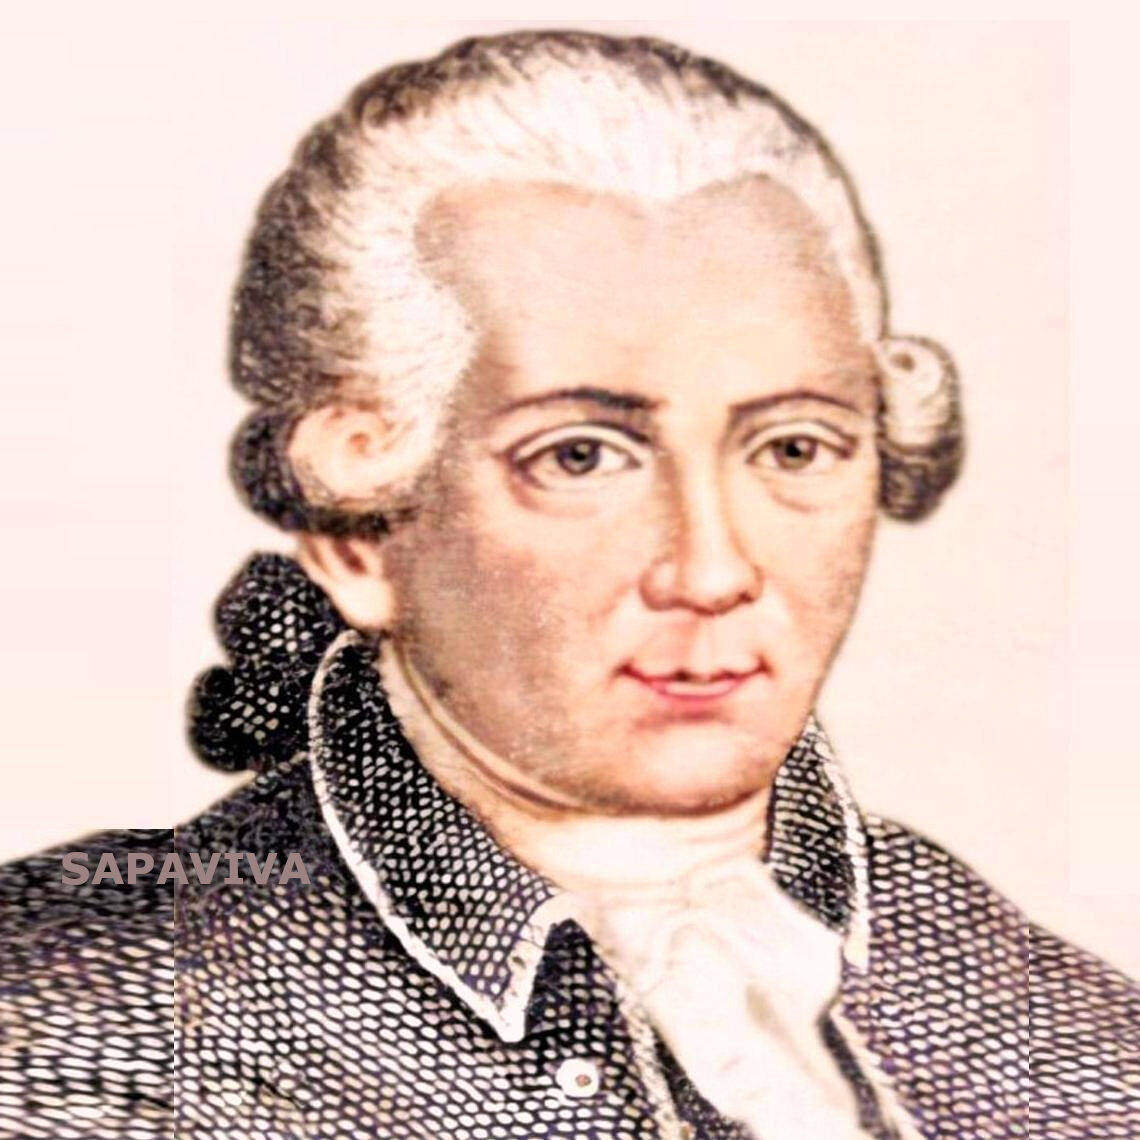
\includegraphics[width=1.875in,height=\textheight]{chapters/images/people/Lambert.png}

}

\caption{\label{fig-lambert}Johann Lambert. His ideas were spread
widely.}

\end{figure}%

Lambert worked on many topics concerning geometric optics, and he
contributed an important book \textbf{Photometria} that incorporated
many important geometric ideas, explaining the relative brightness of
objects as seen from different points of view. Using his excellent
mathematics, and the assumption that light travels in straight lines, he
showed that illumination is - proportional to the strength of the
source, - inversely proportional to - the square of the distance of the
illuminated surface, and - the
\href{https://en.wikipedia.org/wiki/Lambert\%27s_cosine_law}{sine of the
angle} of inclination of the light's direction to that of the surface.
He also wrote a classic work on
\href{https://en.wikipedia.org/wiki/Perspective_(visual)}{perspective}
and contributed to
\href{https://en.wikipedia.org/wiki/Geometrical_optics}{geometrical
optics}.

I was interested to learn that Lambert was the first to show that
\(\pi\) is an irrational number, a claim that the great Euler sought to
prove as well.

\end{minipage}%
\end{tcolorbox}

\begin{figure}

\centering{

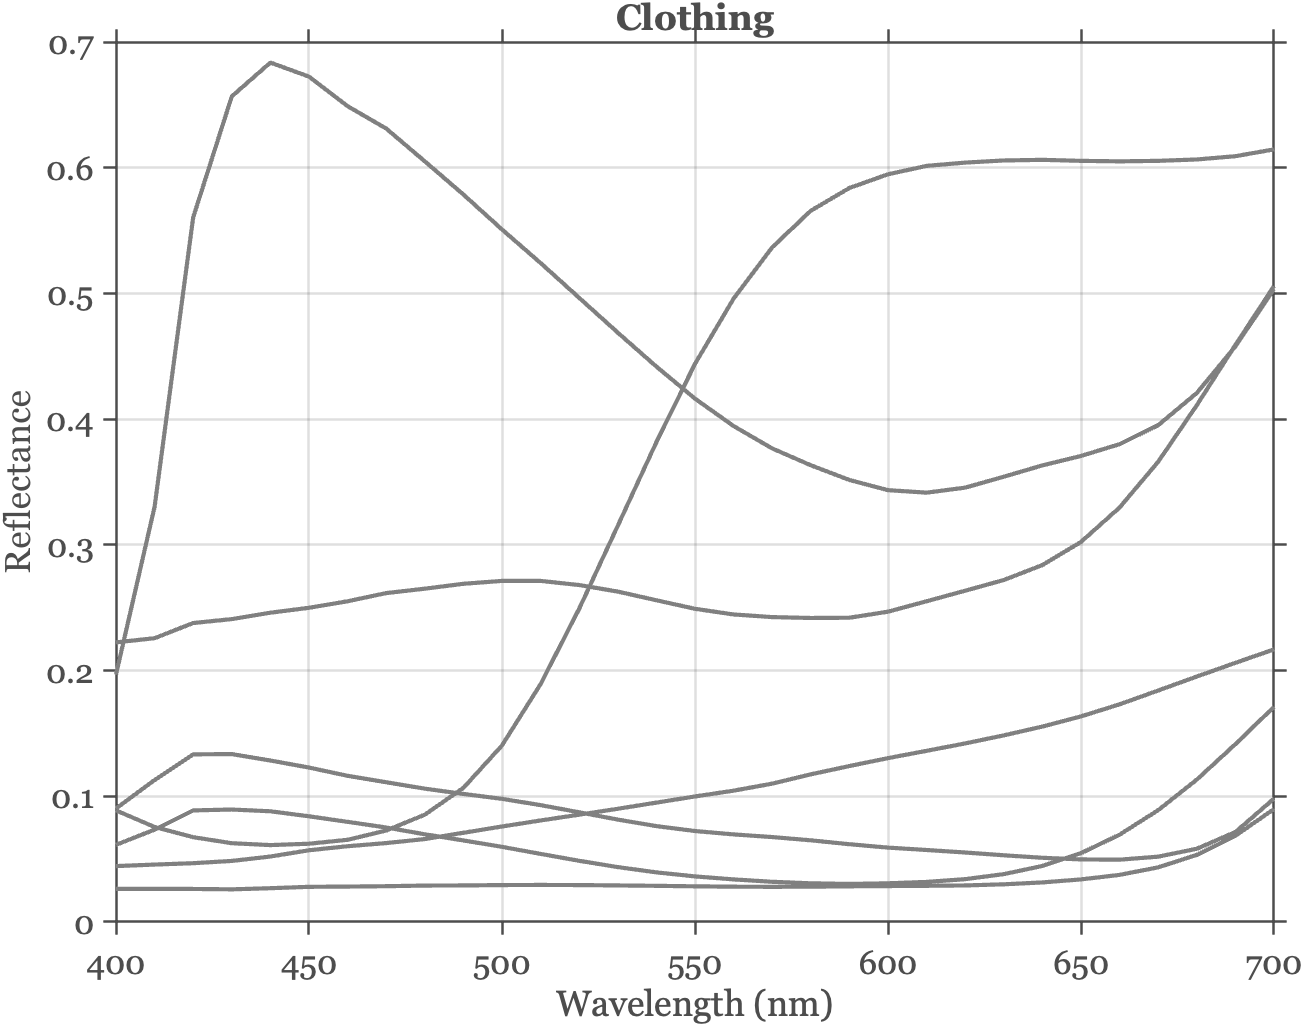
\includegraphics[width=0.6\textwidth,height=\textheight]{chapters/images/lightfields/04-spectral/01-reflectance-clothes.png}

}

\caption{\label{fig-reflectance-cloths}Sample spectral reflectance
functions of clothing. The fraction of reflected light,
wavelength-by-wavelength, is between 0 and 1. Such smooth spectral
reflectance curves are typical of many surfaces. Surfaces that are not
diffuse can be modeled as having a diffuse component with a smooth
spectral reflectance.}

\end{figure}%

We can summarize the spectral reflectance of a diffuse material
relatively simply because we do not need to specify the input and output
angles. We only need to measure the fraction of incident light, for each
wavelength, is reflected. This is called the spectral reflectance
function. In the visible band these functions are often smooth, and it
is possible to summarize them using only a few parameters. It is not
realistic to sample all possible surfaces, but we can consider surfaces
in a particular context (e.g, walking in a forest, clothing, the
interior of a commercial office building, driving on a highway, or
medical images of the body). The likely surfaces in any particular
context can be usefully summarized with a linear model Hardeberg (2002).
The number of basis functions needed will depend on the task
requirements (e.g., 5\% or 1\% accuracy). But the general usefulness of
a linear model approximation as a computational tool is not in doubt.

Over the decades a number of imaging groups have measured the
reflectance of many types of materials, including paints, minerals,
plants, clothing, and various biological specimen such as skin and
teeth. Government agencies, particularly those involved in remote
sensing, have measured the reflectance of many materials that might be
seen in satellite images. As a general rule, the spectral reflectances
of the samples reported in the literature are approximated to an
accuracy of a few percent by linear models using between 3 and 8 basis
functions.

A Finnish group, for example, measured 1269 different color swatches
from the Munsell Book of Colors. This widely used book spans a wide
range of color samples that provides designers with a method for
identifying, selecting, matching, and communicating about color.
Parkkinen et al. (1989) made their spectral measurements at 1 nm
resolution. A linear model using three basis functions fits all the
measurements with an error of about 2.5\%. A linear model with 5 basis
functions fits the data to within about 1\%. This accuracy is usually
often enough for image systems applications
(Figure~\ref{fig-reflectance-bases} A).

The linear models for diffuse surface reflectance of several types of
common materials are similar (Figure~\ref{fig-reflectance-bases}). The
data from Vrhel and colleagues Vrhel et al. (1994), included in ISETCam,
measures a few dozen surfaces from several different groups (paint,
natural objects, man-made objects, food). It is likely the authors chose
the samples to have similar means and a broad representation of color
appearances. For this sampling strategy, the first component will
necessarily be similar. BUt the 2nd and 3rd basis functions are also
similar, and this is less likely to be a selection artifact. Rather, the
similarity arises because the diffuse spectral reflectance functions are
very smooth functions wavelength Maloney (1986).

\begin{figure}

\centering{

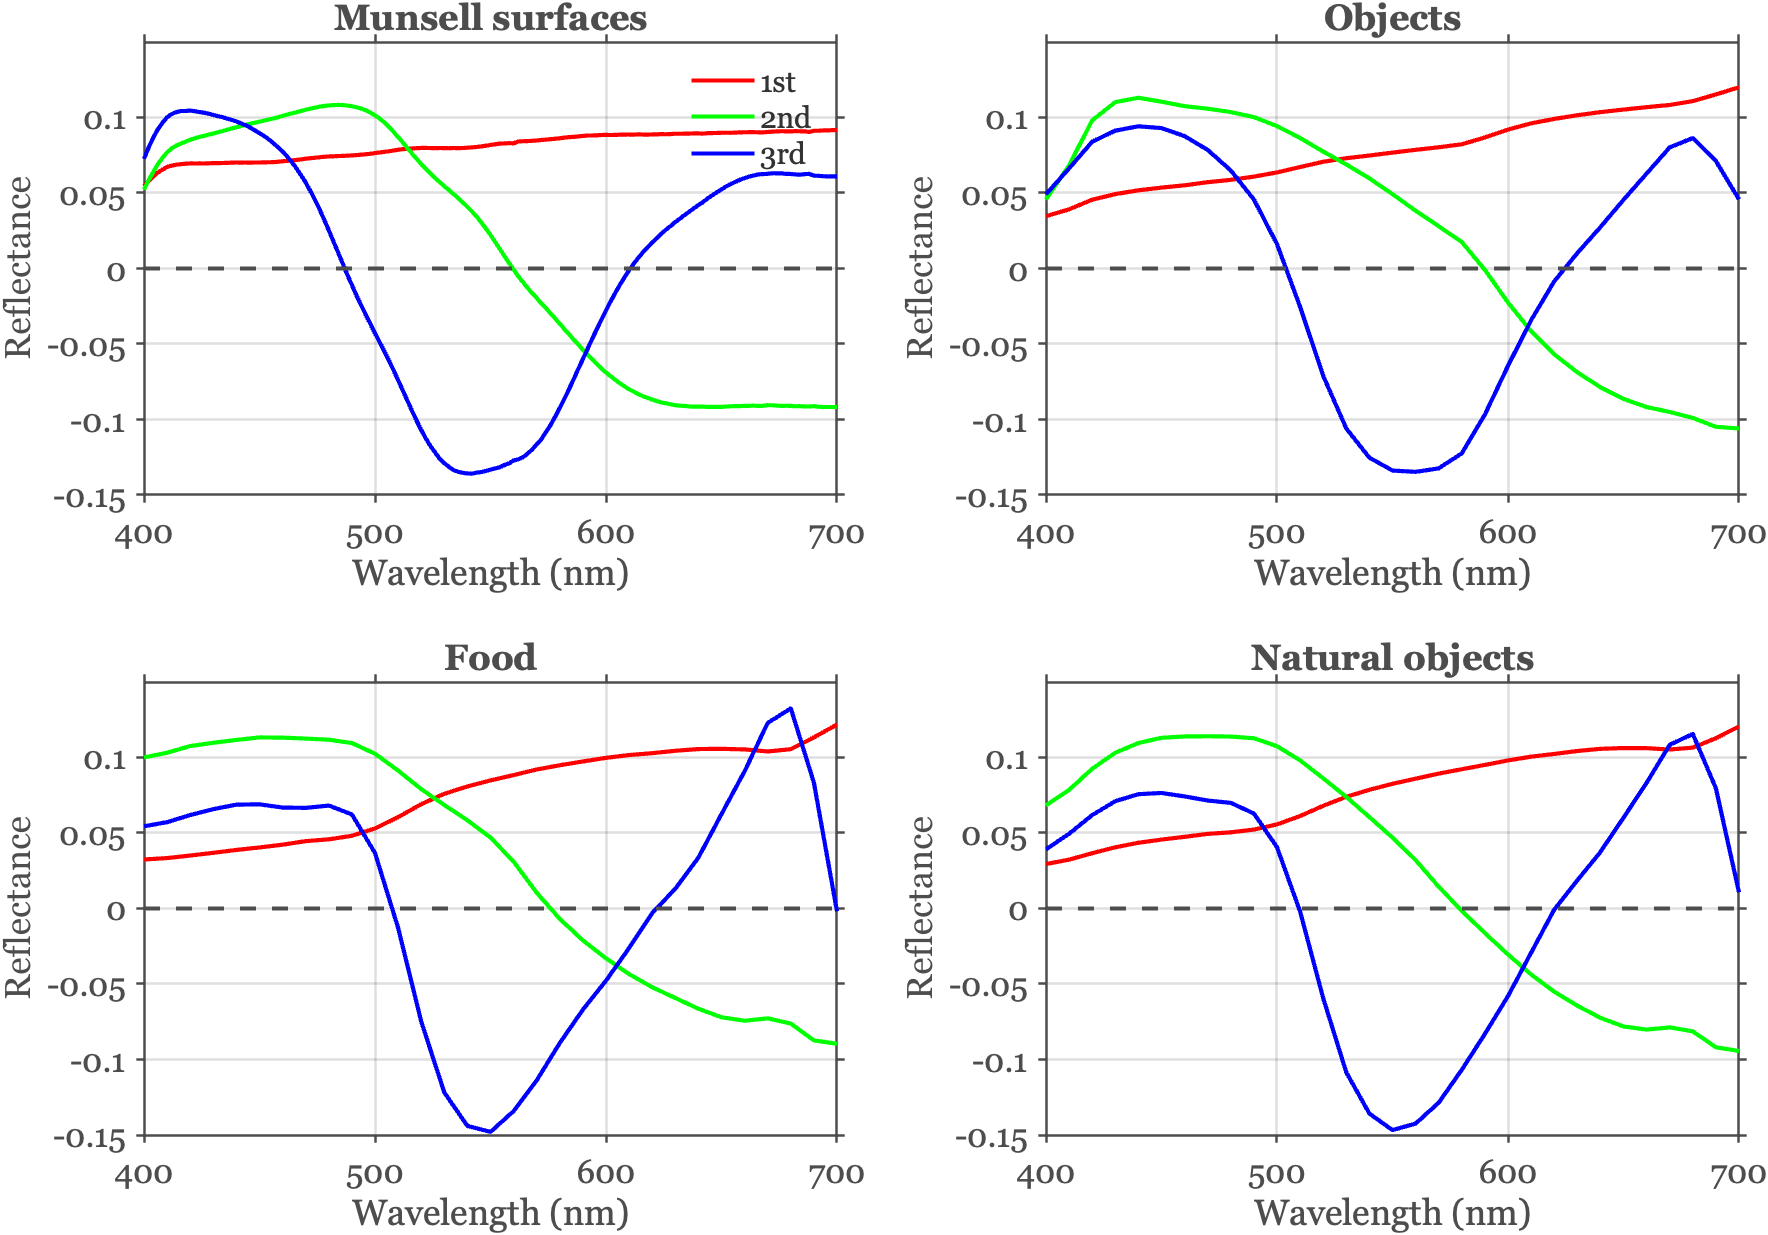
\includegraphics[width=0.8\textwidth,height=\textheight]{chapters/images/lightfields/04-spectral/01-reflectance-bases.png}

}

\caption{\label{fig-reflectance-bases}Three basis functions comparing
the basis functions derived from the Parkkinen et al. (1989) Munsell
Color Book data (upper left) and three different categories of
materials. The basis functions are not identical, but they have many
similarities, including the wavelengths of the zero-crossings of the 2nd
and 3rd basis functions. Data from Vrhel et al. (1994) and distributed
in ISETCam.}

\end{figure}%

\section{Specular reflection (mirror)}\label{specular-reflection-mirror}

The conceptual opposite of diffuse reflection is mirror reflection. In
this case, an incident light ray from one direction reflects from the
surface in just one direction. The geometry of mirror reflection is
shown in Figure~\ref{fig-mirror-reflection}. The incident ray, reflected
ray, and surface normal all lie in the same plane (the \textbf{plane of
incidence}). The angle of incidence is equal to the angle of reflection,
and the surface normal acts as a line of symmetry in the plane of
incidence.

\begin{figure}

\centering{

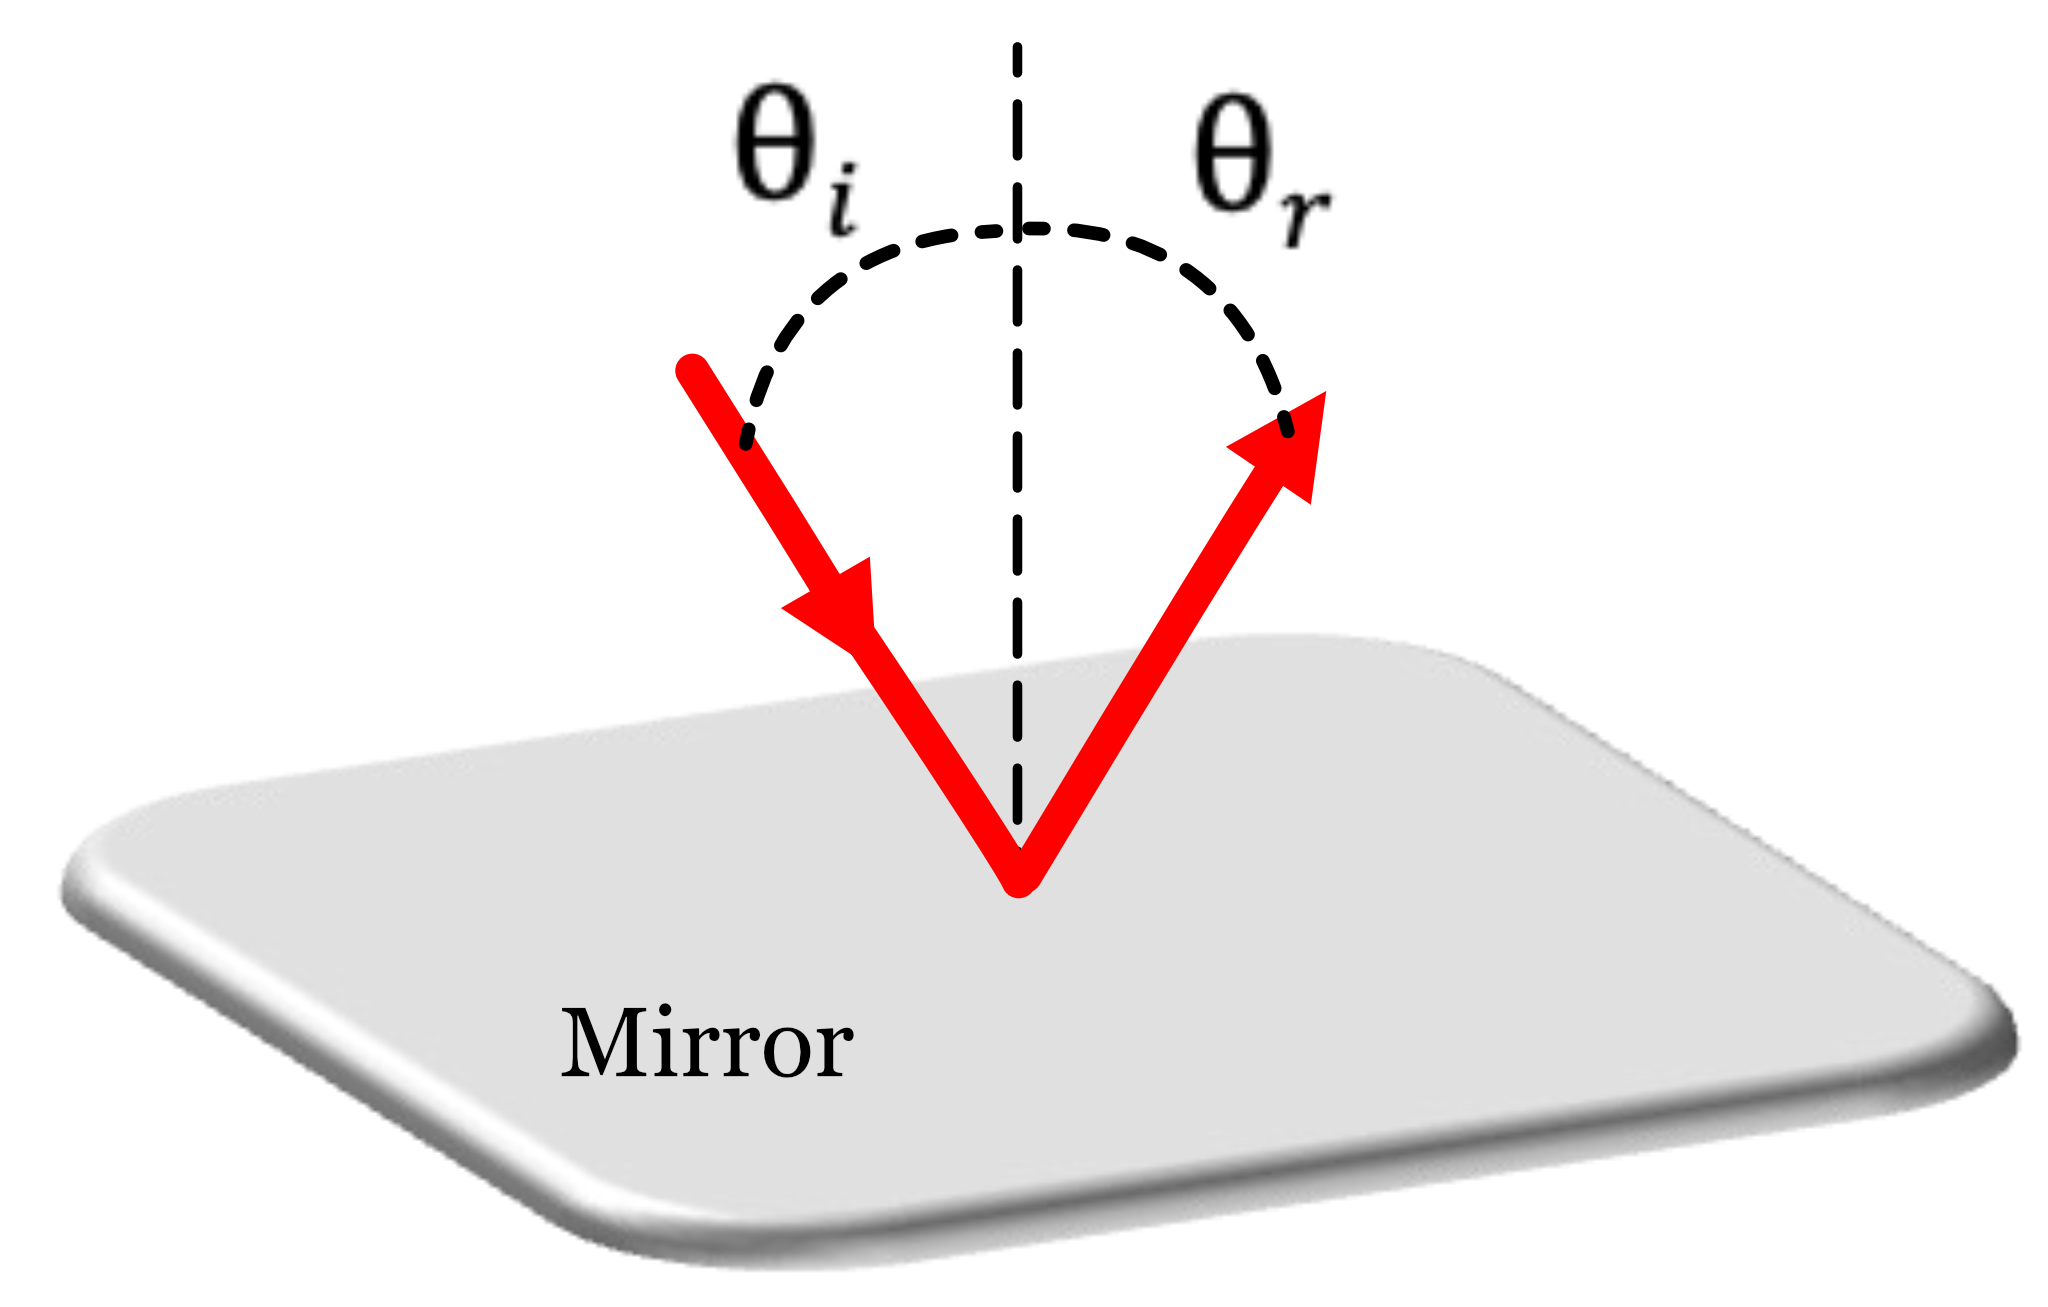
\includegraphics{chapters/images/lightfields/04-spectral/mirror-reflection.png}

}

\caption{\label{fig-mirror-reflection}Geometry of mirror reflection. The
incident (blue) and reflected (red) ray have a component parallel to the
surface normal and a component in the surface plane. The component in
the surface plane is the same; but the component in the normal direction
is sign-reversed (points in the opposite direction). The ray angles with
respect to the surface normal of the two rays is matched \(\theta_i\) =
\(\theta_r\).}

\end{figure}%

It is useful to consider vector components of the incident and reflected
ray separately. Suppose that the incident light comes from a direction
represented by the unit vector \(\mathbf{i}\), and the surface normal
vector is \(\mathbf{n}\). The direction of the reflected ray,
\(\mathbf{r}\) is calculated this way:

\begin{equation}\phantomsection\label{eq-mirror}{
\mathbf{r} = \mathbf{i} − 2 (\mathbf{i} \cdot \mathbf{n}) \mathbf{n}
}\end{equation}

The term (\(\mathbf{i} \cdot \mathbf{n}\)) is the projection of the
incident ray onto the normal ray. We subtract twice that amount from the
incident ray, which flips this component. The component of the incident
and reflected rays that is parallel to the surface are the same. The net
effect is that the incident and reflected rays form equal angles on
opposite sides of the surface normal.

The light reflected at the interface of the surface does not interact
with the material. Thus the spectral power distribution of a mirror
reflection is approximately equal to the spectral power distribution of
the incident radiance.

Common mirrors are close to perfect specular reflectors in the sense
that a very small set of collimated rays is reflected over a very small
angle of output rays. There are only small deviations from slight
surface imperfections. For scientific applications this approximation
may not be adequate, and additional steps are taken to polish mirrors,
making them increasingly perfect.

Many materials are approximately specular, but not perfectly so. In
these materials a narrow bundle of incident rays is reflected mainly in
the specular direction, but there is some spread of the reflected rays.
Figure~\ref{fig-specular-diffuse-retro} compares different conditions,
including a diffuse reflectance, nearly perfect specular, and mostly
specular case.

\begin{figure}

\centering{

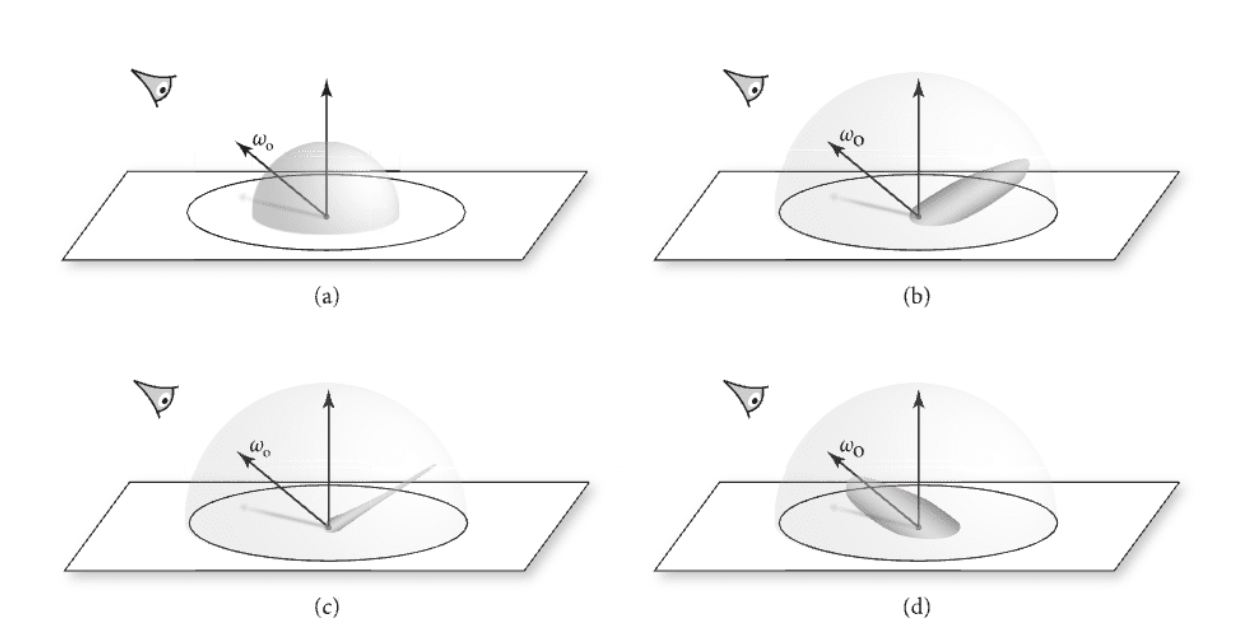
\includegraphics{chapters/images/lightfields/04-spectral/specular-diffuse-retro.png}

}

\caption{\label{fig-specular-diffuse-retro}Comparisons of (a) diffuse,
(b) glossy specular, (c) perfect specular, and (d) retroreflective
materials. Figure 9.1 from PBR book.
https://www.pbr-book.org/4ed/Reflection\_Models}

\end{figure}%

The figure includes a fourth interesting case: retroreflective
materials. For these materials the reflected ray is sent back in the
same direction as the incident ray. These materials can be created by
embedding small, spherical, glass beads with a metallic back surface
into the material Figure~\ref{fig-retroreflective-glass-beads}. The
glass beads refract the incident ray, the metallic surface returns the
ray, which is again refracted, so that the net effect effect is the
reflected ray is returned in the direction of the incident ray. Glass
beads with a metallic backing are often built into road markings and
road signs. Light from a car's headlight is scattered back towards the
driver, increasing the visibility of the road marking or sign during
nighttime driving.

\begin{figure}

\centering{

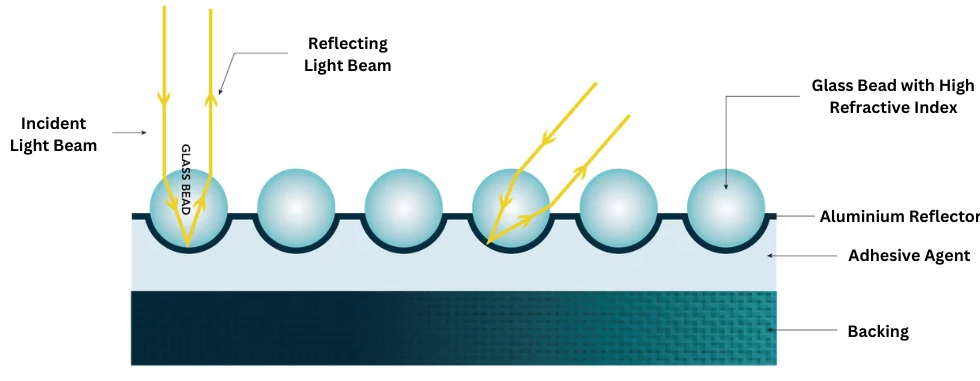
\includegraphics{chapters/images/lightfields/04-spectral/01-retroreflective-glass-beads.png}

}

\caption{\label{fig-retroreflective-glass-beads}Comparisons of (a)
diffuse, (b) glossy specular, (c) perfect specular, and (d)
retroreflective materials. Figure 9.1 from PBR book.
https://www.pbr-book.org/4ed/Reflection\_Models.
https://tccfcct.com/blogs/equipment/all-you-need-to-know-about-reflective-materials-in-high-visibility-safety-apparel}

\end{figure}%

https://docs.google.com/document/d/1BtxldFF14EY4eC9x6KI9cy1RF4GJAy-e7UAgdJ5YsfI/edit?usp=sharing

\section{Dichromatic reflectance model
(DRM)}\label{dichromatic-reflectance-model-drm}

The dichromatic reflectance model (DRM) is another useful surface
reflectance model that serves as an approximation for light reflected
from \textbf{inhomogeneous dielectric materials} (non-conductors like
plastics, paints, wood, skin, etc.). The model approximates reflectance
as a weighted sum of a diffuse term and a glossy specular term. This
model is used in computer vision applications where the user would like
to identify specular reflections.

A fraction of the incident light is reflected at the surface
(\textbf{interface}). This light has a mirror-like reflectance that
preserves the spectral power distribution and glossy specular spatial
distribution. The remaining fraction of the light passes through the
interface into the (\textbf{subsurface}) where it interacts with the
material's pigments, both by diffuse scattering and absorption. The
subsurface reflectance is usually assumed to be Lambertian, as the
subsurface pigments are randomly positioned and oriented. The reflected
light, \(C(\lambda)\) is the sum of the interface and subsurface terms

\begin{equation}\phantomsection\label{eq-DRM}{
C(\lambda) = m_s(g) I(\lambda) E(\lambda) + m_d(g) D(\lambda) E(\lambda)
}\end{equation}

\(E(\lambda)\) is the spectral power distribution of the light;
\(D(\lambda)\) is the diffuse subsurface reflectance, which is
characteristic of the material. The terms \(m_s(g)\) and \(m_d(g)\) are
geometric scaling factors whose values depend on the illumination and
viewing angles. These angles are ordinarily represented with respect to
the surface normal at the surface point \(g\). The reflected light,
\(C(\lambda)\) is sometimes called the \emph{color signal} because this
spectral radiance is an important contributor to the visual system's
color judgment. (Though, I have friends who object to this term).
\(I(\lambda)\) is the interface spectral reflectance is often assumed to
be constant across wavelengths, which further simplifies the formula

\begin{equation}\phantomsection\label{eq-DRM-simplified}{
C(\lambda) = m_s(g) E(\lambda) + m_d(g) D(\lambda) E(\lambda)
}\end{equation}

The DRM is used in computer vision algorithms such as illuminant
estimation, specular highlight identification and removal, and material
classification. It is, however, limited because it does not accurately
model complex surfaces. Also, it is difficult to apply to scenes with
multiple light sources or very large light sources, such as scenes with
light sources that span the sky.

\begin{tcolorbox}[enhanced jigsaw, colframe=quarto-callout-note-color-frame, left=2mm, opacityback=0, colback=white, arc=.35mm, toprule=.15mm, rightrule=.15mm, leftrule=.75mm, bottomrule=.15mm, breakable]
\begin{minipage}[t]{5.5mm}
\textcolor{quarto-callout-note-color}{\faInfo}
\end{minipage}%
\begin{minipage}[t]{\textwidth - 5.5mm}

\vspace{-3mm}\textbf{DRM Illuminant estimation}\vspace{3mm}

Suppose the interface reflectance, \(I(\lambda)\) is approximately
constant so that we accept Equation~\ref{eq-DRM-simplified}. If we
measure the reflected light from a DRM material at a few angles, we will
obtain values that differ because of the geometric terms, \(m_s\) and
\(m_d\). These different estimates can be represented as a
two-dimensional linear model.

The linear terms we estimate from any single surface, say using
principal components, may not be precisely aligned with \(E(\lambda)\)
and \(D(\lambda) E(\lambda)\). But if there are two or more different
dichromatic reflectance type materials near one another, their linear
models must have a shared dimension, \(E(\lambda)\). Thus, we can
estimate the principal components of both surfaces, and then find the
vector equal to the intersection of these linear models, we will recover
the local spectral power distribution of the illuminant.

\end{minipage}%
\end{tcolorbox}

\section{Bidrectional reflectance distribution function
(BRDF)}\label{sec-properties-brdf}

The \emph{bidirectional reflectance distribution function} (BRDF)
characterizes how light rays of wavelength \(\lambda\), incident at the
surface at an angle \(\omega_i\), are reflected. The reflected, outgoing
light is specified at all angles \(\omega_o\). Both \(\omega_i\) and
\(\omega_o\) are measured with respect to the surface normal. We can
write the intensity as a function of input and output angles as the
function \(B(\omega_i,\omega_o,\lambda)\). The reciprocity of principle
of light\footnote{The principle states that if a ray of light travels
  from point A to point B through any optical system, then the same ray
  can travel in the reverse direction from B to A, following the same
  path. This remains true regardless of the complexity of the optical
  system, including reflections, refractions, and scattering. The
  concept is often attributed to Hermann von Helmholtz, who formally
  stated it in his 1856 book Handbook of Physiological Optics Helmholtz
  (1896).} implies that the BRDFs, with only a few exceptions, obey this
symmetry relationship.

\begin{equation}\phantomsection\label{eq-BRDF1}{
B(\omega_i,\omega_o,\lambda) = B(\omega_o,\omega_i,\lambda)
}\end{equation}

Each of the direction vectors is specified by two parameters, typically
defined with respect to the surface normal. One parameter is the angle
around the surface normal (azimuth) \(\phi_i, \phi_o\), and the second
is the elevation \(\theta_i, \theta_o\) of the ray. We conventionally
describe the BRDF with three parameters, but there are really five
parameters in there. That makes the BRDF tedious to measure.

The instrument used to measure the BRDF is called a gonioreflectometer.
The instrument has a light source that can be positioned to illuminate
the surface at many different angles (typically on a sphere), and a
detector that can be positioned at many locations on the sphere. There
are many different designs for \emph{gonioreflectometers}. The one in
Figure~\ref{fig-gonioreflectometer} shows a surface is placed on a stage
that can be rotated. The light and camera are on two arms whose
positions can be controlled, sweeping out the possible angles for the
incident and reflected light. To measure the reflectance of a surface
requires calibrating the amount of incident light, say by making a
measurement with a perfect, white diffusing surface, and then making a
second measurement with the material of interest. The ratio of the
responses is the reflectance. The same calibration measurement can be
re-used for multiple materials of interest.

\begin{figure}

\centering{

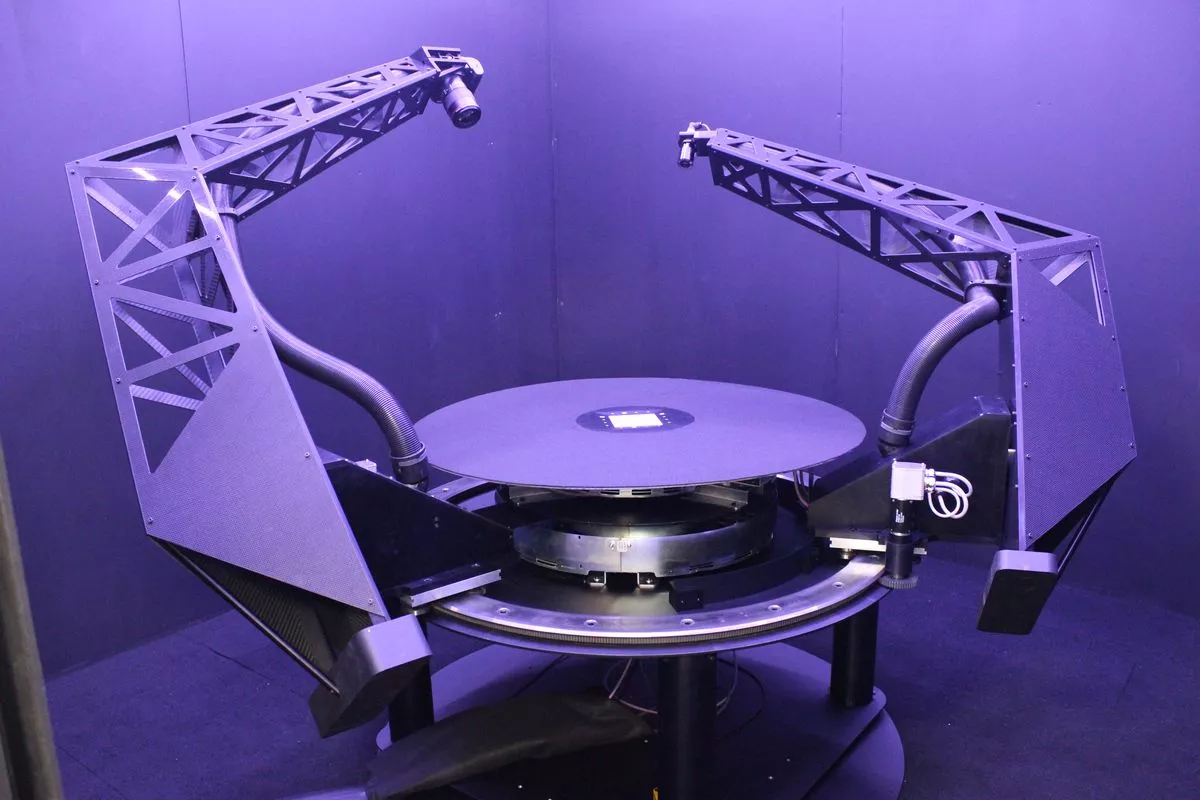
\includegraphics[width=0.75\textwidth,height=\textheight]{chapters/images/lightfields/04-spectral/01-gonioreflectometer.png}

}

\caption{\label{fig-gonioreflectometer}Example of a
\textbf{gonioreflectometer}. The light source and detector are on robot
arms that can be positioned around the surface. If we fix the wavelength
and angle of the incident light ray, we can specify the relative
intensity of the reflected light as an image that spans the two angle
parameters}

\end{figure}%

The input and output angles are 2-vectors and the BRDF is a scalar
function. We can make all of the angles explicit this way.

\begin{equation}\phantomsection\label{eq-BRDF2}{
B(\omega_i, \omega_o, \lambda) = f_r(\phi_i,\theta_i,\phi_o,\theta_o,\lambda)
}\end{equation}

\subsection{Theoretical BRDF}\label{theoretical-brdf}

Cook Torrance mainly here.

\subsection{Data driven BRDF}\label{data-driven-brdf}

There are papers measuring BRDFs and modeling them using linear models
and nonlinear models. Data driven approach.

Matusik et al. (2003) Tongbuasirilai et al. (2020)

There is a MERL database online.

\chapter{Spatial regularities}\label{sec-spatial-regularities}

\section{Spatial regularities
overview}\label{sec-spatial-regularities-overview}

Something about fractals. Textures. Other stuff. Simoncelli and
Olshausen (2001) Geisler (2008) Ruderman and Bialek (1994)

\subsection{Fractals and Power Spectra scale
invariance}\label{sec-fractals}

The scale invariance of natural images arises from their power-law
spectral decay, which mathematically ensures statistical consistency
across spatial scales. The connection between 1/f\^{}α spectra and scale
invariance can be expressed through:

The power spectrum of natural images follows:

\[
P(\omega) \propto \frac{1}{|\omega|^{2-\eta}} \quad \text{where } \eta \approx 0.8\text{--}1.5
\]

Here, \(\omega\) represents spatial frequency magnitude, and \(\eta\)
controls the decay rate\footnote{https://people.csail.mit.edu/danielzoran/zoranweiss09.pdf}\footnote{https://web.mit.edu/torralba/www/ne3302.pdf}\footnote{https://www.sciencedirect.com/science/article/pii/0042698996000028}.

For scale invariance under spatial scaling \(x \to \lambda x\), the
power spectrum must satisfy:

\[
P(\lambda\omega) = \lambda^{-\kappa}P(\omega)
\]

Substituting the power-law form:

\[
P(\lambda\omega) = \frac{1}{|\lambda\omega|^{2-\eta}} = \lambda^{-(2-\eta)}P(\omega)
\]

This matches the scale-invariance condition with \(\kappa = 2-\eta\),
demonstrating that statistical properties remain consistent across
scales\footnote{https://people.csail.mit.edu/danielzoran/zoranweiss09.pdf}\footnote{https://web.mit.edu/torralba/www/ne3302.pdf}\footnote{http://vigir.missouri.edu/\textasciitilde gdesouza/Research/Conference\_CDs/IEEE\_ICCV\_2009/contents/pdf/iccv2009\_285.pdf}.

\textbf{Fractal connection} The power-law exponent relates to fractal
dimension \(D\) through:

\[
D = 3 - \frac{\eta}{2}
\]

where \(D\) quantifies space-filling characteristics. Natural images
typically exhibit \(D \approx 2.2\text{--}2.6\), consistent with their
1/f\^{}α spectra\footnote{https://people.csail.mit.edu/danielzoran/zoranweiss09.pdf}\footnote{https://www.nature.com/articles/srep46672}.

This mathematical framework shows that 1/f\^{}α spectra inherently
encode fractal, scale-invariant structure - the same statistical
regularities appear whether analyzing fine details or coarse features of
natural scenes\footnote{https://people.csail.mit.edu/danielzoran/zoranweiss09.pdf}\footnote{https://web.mit.edu/torralba/www/ne3302.pdf}\footnote{http://vigir.missouri.edu/\textasciitilde gdesouza/Research/Conference\_CDs/IEEE\_ICCV\_2009/contents/pdf/iccv2009\_285.pdf}.

⁂

\subsection{Natural scenes and the 1/f spatial frequency
falloff}\label{natural-scenes-and-the-1f-spatial-frequency-falloff}

Who first pointed this out? Relationship to the scale invariant idea of
fractals, and the fractal nature of many things.

Ruderman and Bialek paper on natural image statistics.

Field, Olshausen

Lee et al. (2001)

\subsection{Natural scenes: The dead leaves
model}\label{natural-scenes-the-dead-leaves-model}

Jon's Matlab script as a basis for discussing this.
\href{https://github.com/isetbio/isetbio/blob/main/scripts/oneoverf/s_oneOverF1D.m}{Software
from Jon showing 1/f issues.}

Also, the deadleaves function in ISETCam.

\part{Optics}

\chapter{Geometric optics}\label{sec-geometric-optics}

\section{Geometric optics overview}\label{geometric-optics-overview}

Modeling light as rays is a useful approximation for many calculations.
This method enables us to use simple geometric calculations (e.g.,
similar triangles), to derive many properties of simple lenses. For this
reason this approach is also called \textbf{geometric optics}. In this
chapter we use geometric optics to describe the simplest image forming
optics, a \textbf{pinhole}. After understanding the logic of modeling
using rays and pinholes, I also explain the limitations of the ray model
and why we will also model light as waves. Finally, I discuss the key
concept of the \textbf{point spread function}, which plays a role in all
the different modeling approaches. I extend the geometric optics
calculations in the next few chapters, before turning to linear systems
theory and wavefronts (Fourier optics).

\section{Pinhole optics}\label{pinhole-optics}

If we model light as a collection of rays, it is easy to understand why
imaging through a pinhole produces an image
(Figure~\ref{fig-pinhole-image}). The figure shows a set of
\emph{objects} on the left. The camera is a dark chamber with only a
pinhole opening. The \emph{image} is formed on the planar surface, at
the right. The light rays travel in a straight line, so only a small
subset of the rays from each object passing through the pinhole. We can
trace the light path by starting at a point on the image and drawing a
straight line into the object space. The geometry illustrates how the
rays from adjacent objects arrive at adjacent positions in the image
plane, forming a reversed and inverted image.

\begin{figure}

\centering{

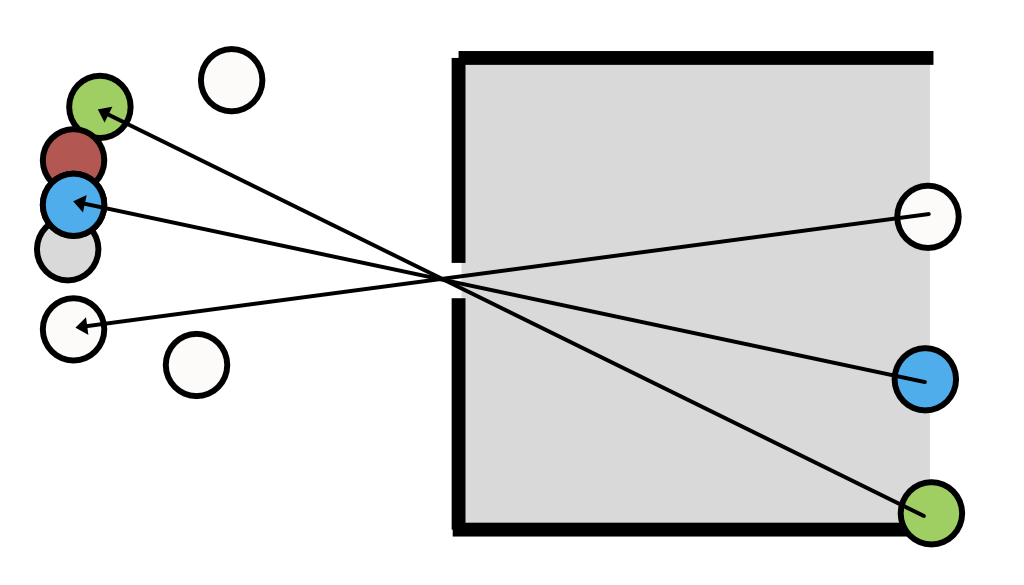
\includegraphics[width=0.6\textwidth,height=\textheight]{chapters/images/optics/06-geometric/pinhole-image.png}

}

\caption{\label{fig-pinhole-image}A pinhole makes an image.}

\end{figure}%

If the pinhole is small, each image point receives rays from a small
region in object space (Figure~\ref{fig-pinhole-blur}). As we increase
the pinhole diameter, each image point receives rays from larger regions
on the objects. If multiple objects contribute rays to an image point,
the image will be blurry. Conversely, according to the ray model,
reducing the pinhole size should sharpen the image.

\begin{figure}

\centering{

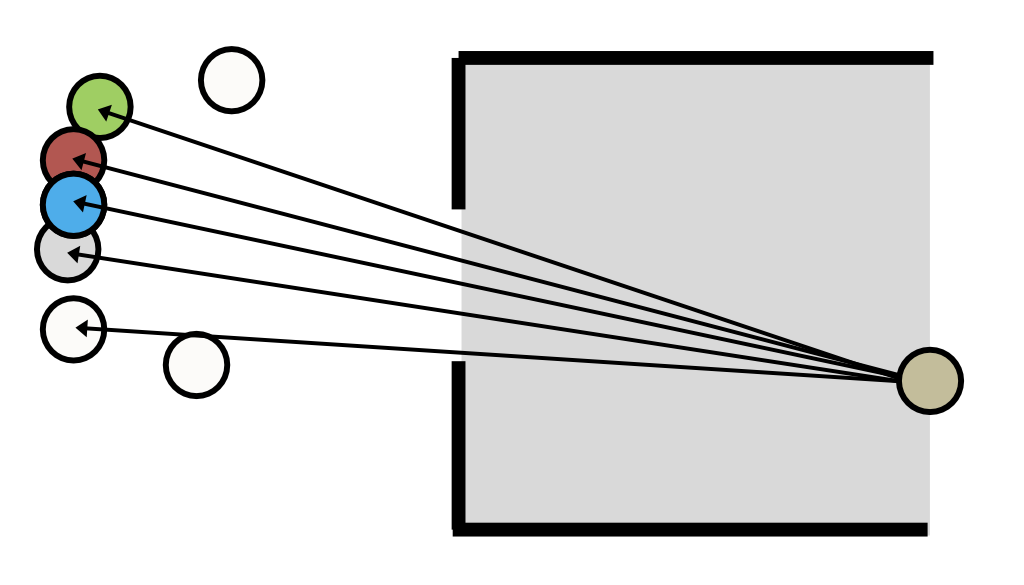
\includegraphics[width=0.6\textwidth,height=\textheight]{chapters/images/optics/06-geometric/pinhole-blur.png}

}

\caption{\label{fig-pinhole-blur}Why enlarging the pinhole increases the
blur.}

\end{figure}%

\subsection{Parallel (collimated) rays}\label{sec-pinhole-collimated}

The rays from a point on an object often radiate in a wide range of
directions. A special case -that is important in many practical
applications- are the rays from distant points
(Figure~\ref{fig-pinhole-distant}). When the point is far, only a small
angular bundle of rays arrives at the pinhole. When the angle is very
small, the rays are nearly parallel. In that case we say the beam of
light is \textbf{collimated}.

\begin{figure}

\centering{

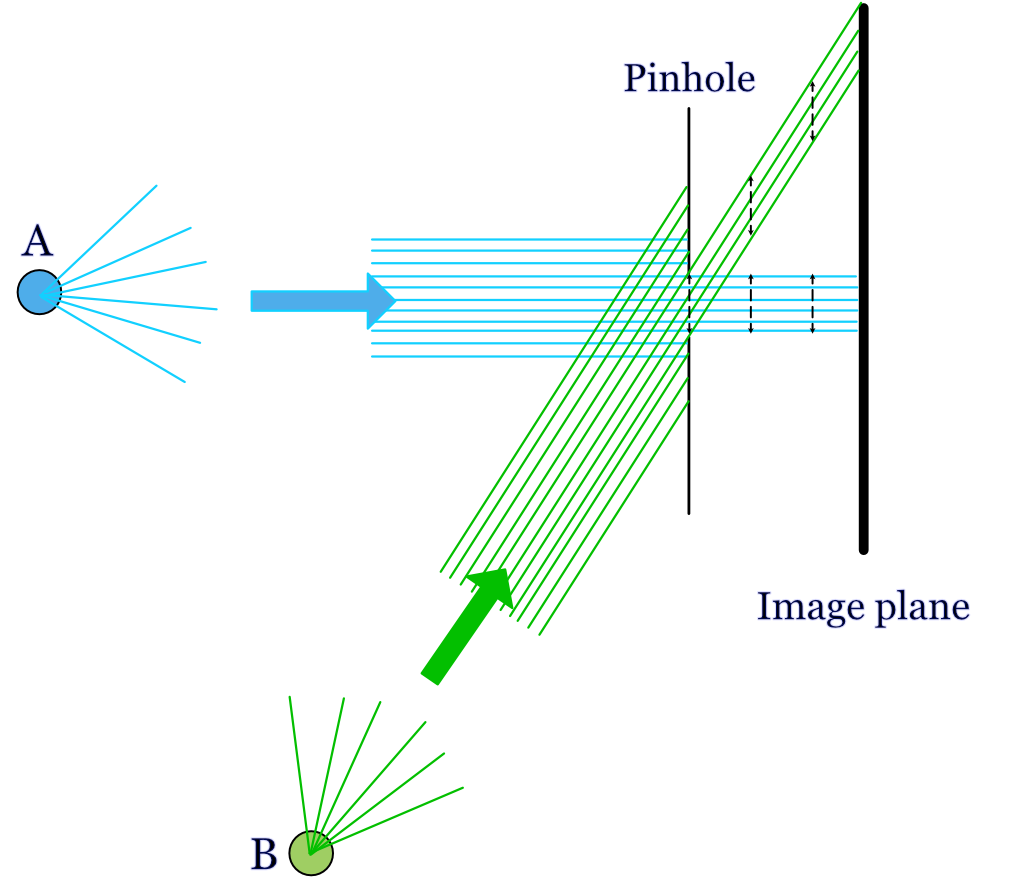
\includegraphics[width=0.6\textwidth,height=\textheight]{chapters/images/optics/06-geometric/pinholePSF.png}

}

\caption{\label{fig-pinhole-distant}Pinhole camera geometry. The rays
from a distant objects arrive in parallel (collaimated) at the pinhole.
If rays travel in straight lines, they would continue to form an image
the size of the pinhole (short dashed black lines). Hence, the size of
the point image would be the same for on-axis (A) and off-axis (B)
points. However, you can see that although I drew the same pattern of
rays for the two points, we expect fewer rays from the off-axis point
(B) to pass through the aperture. Its image will be dimmer.}

\end{figure}%

For an object point, \textbf{A} that is aligned with the pinhole
(on-axis), the ray model of light predicts that the rays will continue
straight through the pinhole aperture and form an image that is very
close to the same size as the pinhole itself. Consider a distant
off-axis point, \textbf{B}. Its rays, too, will start in many directions
and only a narrow, collimated subset of rays will arrive at the pinhole
aperture. Because of the angle between the collimated rays and the
pinhole, a smaller fraction of the rays will pass through the pinhole
aperture. There will be less light from \textbf{B} than from \textbf{A}.
The relative amount of light that makes it through the pinhole depends
on the cosine of the angle between the pinhole and the rays. But the
shape of the image from the two points does not differ. If the pinhole
is circular, on- and off-axis points will produce a circular image with
the same diameter as the pinhole.

Figure~\ref{fig-ayscough} by Ayscough illustrates an image formed by a
complex scene, with many points. Each point in the scene is blurred and
rendered at a unique position. Also, the intensity at each point will be
impacted by its relative angle to the pinhole and image surface. If the
image intensity through the pinhole is adequate, and we do not mind the
blurring, we will have a satisfactory image.

\subsection{Pinhole: Computer graphics}\label{pinhole-computer-graphics}

Pinhole cameras are often used in computer graphics calculations. They
are simple to compute, tracing light from the recording surface (film or
sensor) through the pinhole back into object space. In computer graphics
it is fairly common to aim to render a nice looking image, rather than a
physically accurate image. The pinhole approximation to optics provides
a sharp image with large depth of field that is suitable for many
applications.

It is also possible to use pinhole computations to illustrate the
limitations of this model in real image systems. In
Figure~\ref{fig-pinhole-chessset} I rendered a chess set scene with the
pieces, each a few cm tall, positioned about 0.5 meters from the pinhole
camera. The four pictures were rendered using different pinhole
diameters. The upper left allows only one ray through from each location
in the scene. The aperture diameters for the next three pictures are for
three different pinhole sizes. The images are brighter as the pinhole
size increases. For this example, the image at the two smaller pinhole
sizes are tolerable. Depending on your viewing distance from the screen
or page, the third pinhole image might be usable. But the largest
pinhole, which lets in the most light, loses so much spatial information
that the individual pieces blur together in the image
(Section~\ref{sec-airy-pattern}).

\begin{figure}

\centering{

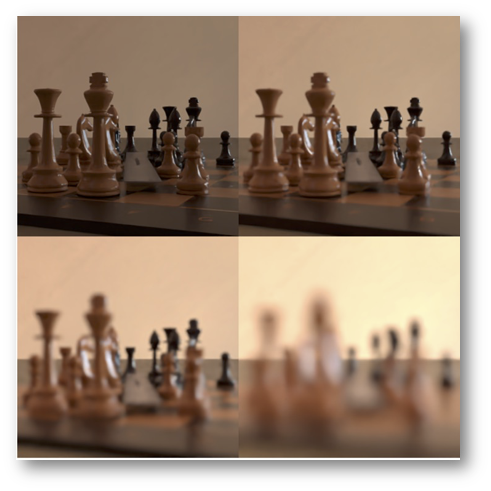
\includegraphics[width=0.8\textwidth,height=\textheight]{chapters/images/optics/06-geometric/01-pinhole-chessset.png}

}

\caption{\label{fig-pinhole-chessset}A simulated scene rendered through
a pinhole camera, using only ray tracing. The size of the pinhole
diameter increases from the upper left to the lower right. The relative
intensity is preserved in the renderings so that the scene becomes
brighter as the pinhole diameter increases. Rendered with (Pharr et al.)
and (2022).}

\end{figure}%

\subsection{Pinholes: real life}\label{pinholes-real-life}

The basic idea of the pinhole camera (also called the \textbf{camera
obscura}) has been known for thousands of years. Surely, many people
noticed the phenomenon in different times and places. We have a record
that the Chinese philosopher Mozi (c.~470--391 BC) wrote that an
inverted image is formed through a pinhole, and moreover he explained
the phenomenon by positing that light travels in straight lines! The
Chinese scientist Shen Kuo (1031--1095) described the process explicitly
in his book Dream Pool Essays, also noting that the image is inverted
because light rays travel in a straight line from the source to the
pinhole and then continue straight to form the image.

The most significant Islamic figure is Ibn al-Haytham (c.~965--1040),
also known as Alhazen. His influential work, the Book of Optics,
provides a comprehensive analysis of the camera obscura phenomenon. He
used the term al-bayt al-muthlim (``the dark room'') to describe the
pinhole camera, and he conducted experiments to demonstrate that a small
hole could project an image of an external scene onto the opposite wall.
Al-Haytham correctly reasoned that the pinhole created a clear image
because it isolates and channels individual light rays from different
points of the object, preventing them from mixing. His work included
many other observations that laid the groundwork for modern optics.

\begin{tcolorbox}[enhanced jigsaw, bottomtitle=1mm, titlerule=0mm, arc=.35mm, colbacktitle=quarto-callout-note-color!10!white, coltitle=black, toprule=.15mm, bottomrule=.15mm, breakable, colframe=quarto-callout-note-color-frame, left=2mm, opacityback=0, colback=white, title=\textcolor{quarto-callout-note-color}{\faInfo}\hspace{0.5em}{Natural pinholes}, opacitybacktitle=0.6, toptitle=1mm, rightrule=.15mm, leftrule=.75mm]

From time-to-time people report on interesting examples of naturally
occurring pinhole cameras. This video shows how the holes at the top of
a curtain produce a series of overlaping images of the street below.

\begin{figure}[H]

\centering{

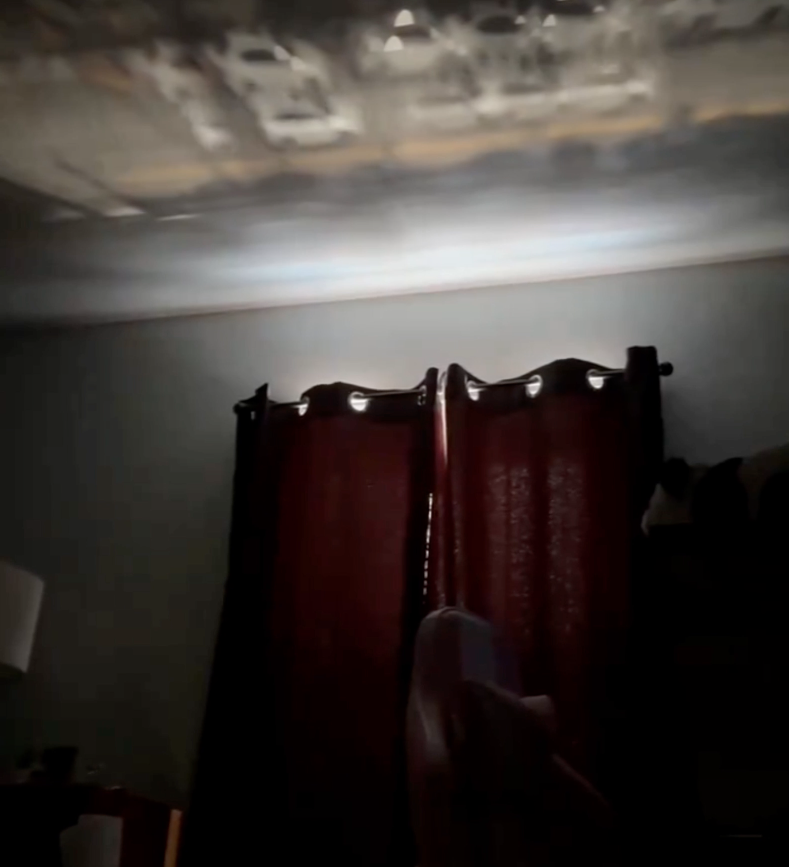
\includegraphics[width=0.4\textwidth,height=\textheight]{chapters/images/optics/06-geometric/pinholes-video-rainmaker-still.png}

}

\caption{\label{fig-pinholes-rainmaker}Video of a natural set of
pinholes at the upper part of the curtain.
(https://x.com/Rainmaker1973/status/1830854129155031206)\{target=\_blank\}}

\end{figure}%

(\href{https://x.com/Rainmaker1973/status/1830854129155031206}{See the
original source})

Antonio Torralba and Bill Freeman and Torralba and Freeman (2012)
described examples of naturally occurring pinhole cameras, and how to
create a pinhole image computationally even when a window is too big to
produce a useful image. They say you can take record the very blurry
image from a large window opening, and then you can put a small occluder
into the window (maybe stand sidewise in the middle of the window) and
take a second image. Then, subtract the two images. By the Principle of
Superposition, the difference image corresponds to the image when the
aperture was the same size as the occluder. This method is more complex
to implement because it involves acquiring two (linear) images and then
subtracting them. And the world might have changed between the time you
took the two image. But it's a good trick for spies who are desperate to
learn where they are being held hostage.

\begin{figure}[H]

\centering{

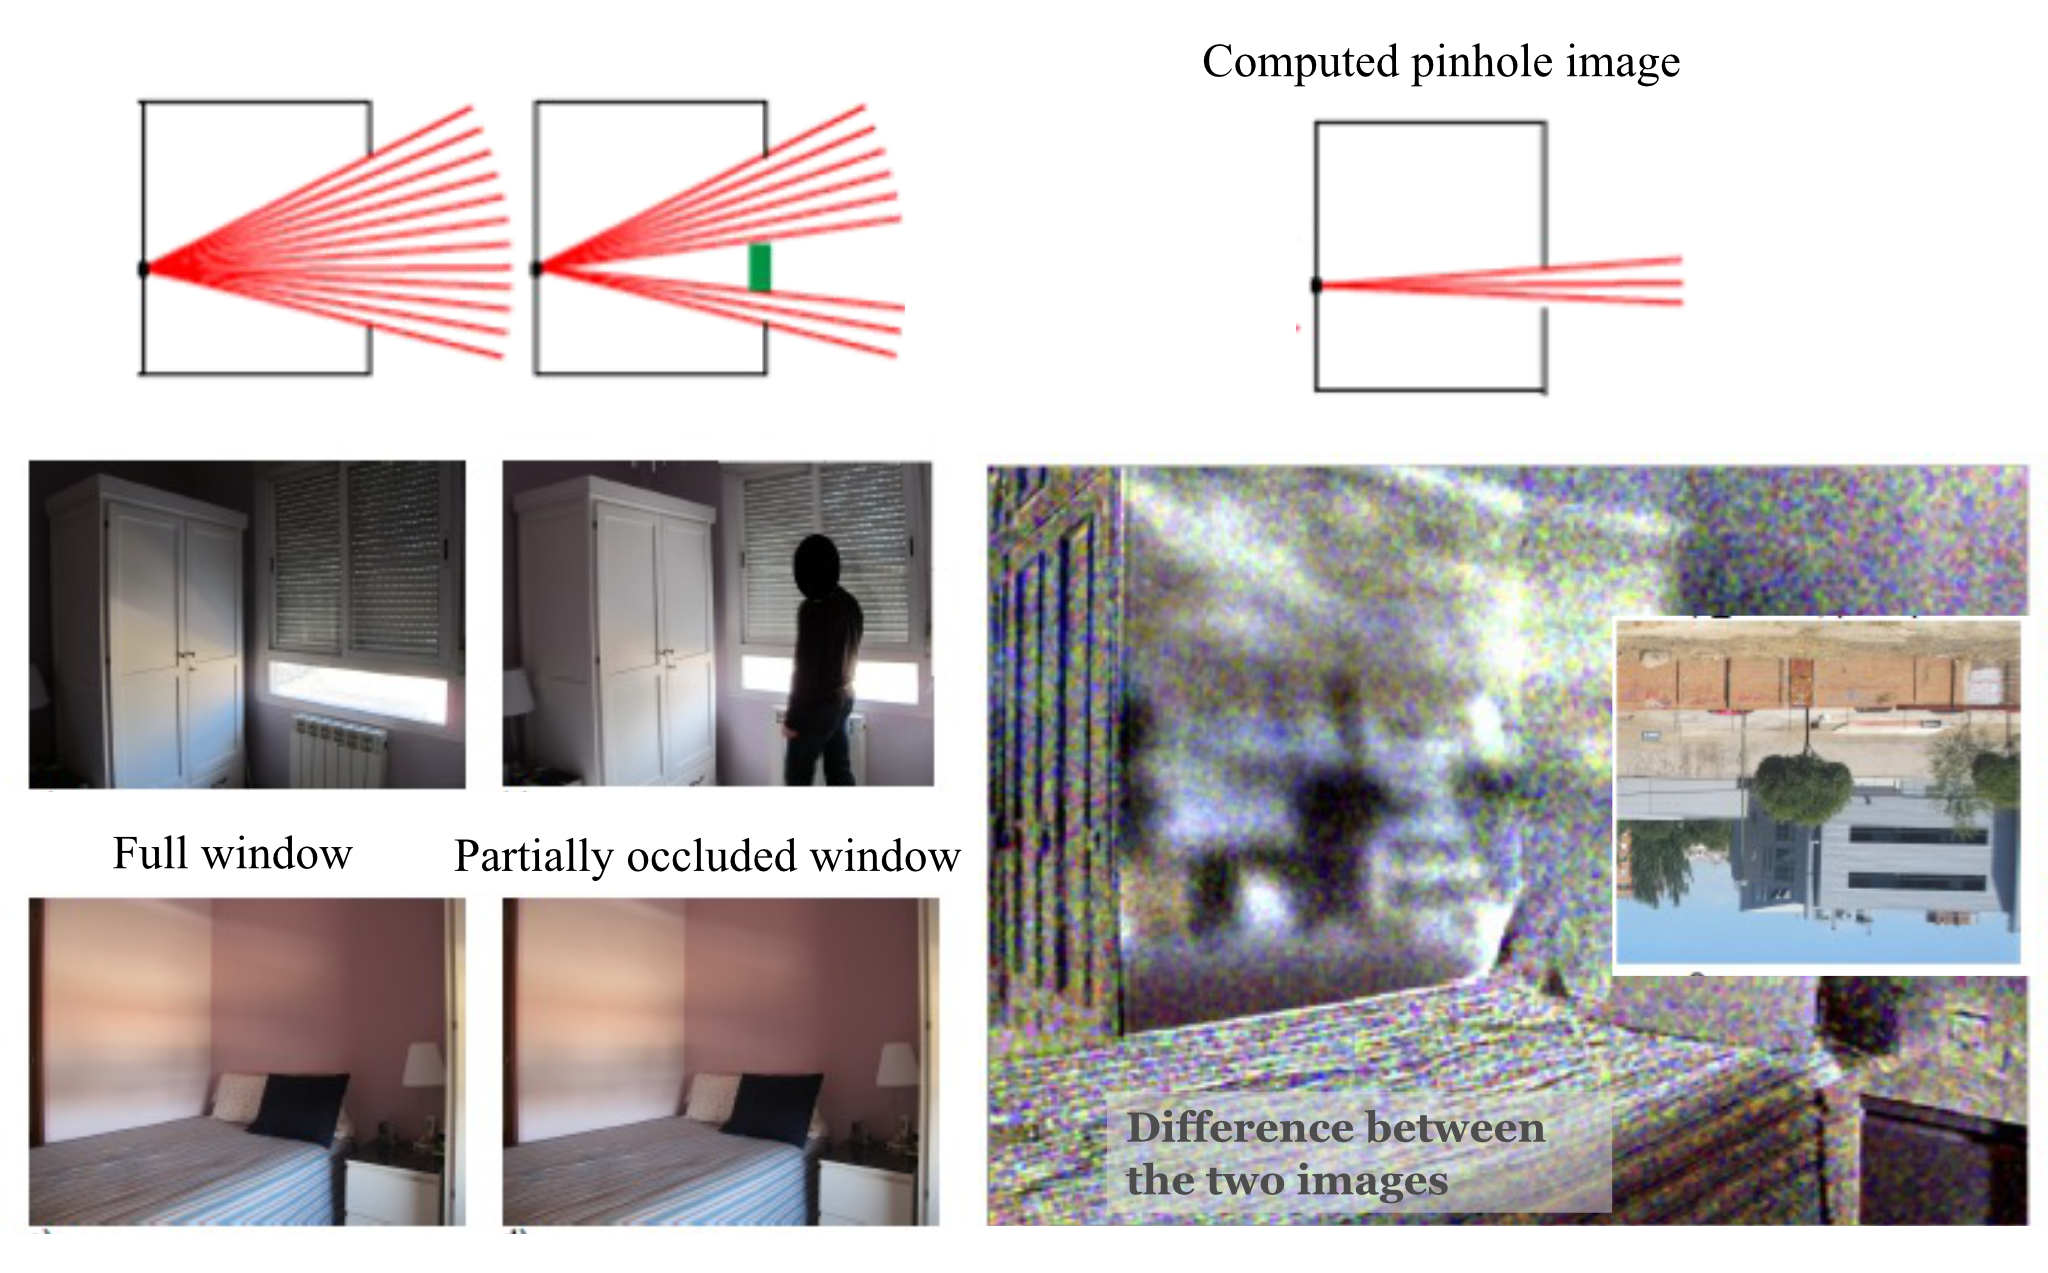
\includegraphics[width=0.8\textwidth,height=\textheight]{chapters/images/optics/06-geometric/torralba.png}

}

\caption{\label{fig-torralba}A pinhole camera image formed by
substracting an image with an occluder (left) from an image without the
occluder (middle). If the two captured images are linear measures of the
photons, then Principle of Superposition implies we can subtract them
and be left with a computed image that we would have obtained with
through the occluded region. The result is a (noisy) image that Torralba
and Freeman call `inverse' inphole camera.}

\end{figure}%

\end{tcolorbox}

// \ldots existing code\ldots{} \#\# Diffraction
\{\#sec-lightfields-diffraction\} Useful as the ray model has been, for
more than 300 years scientists have known that geometric optics is not
completely accurate. Consider the simple prediction of the ray model in
Figure~\ref{fig-ray-wave}. The parallel rays from a point source should
pass through the pinhole and continue in a straight line, forming an
image the size of the pinhole. An observer to the side should see only
darkness, as no rays are heading toward their eyes.

But this isn't what happens. As the Jesuit scientist Francesco Grimaldi,
a contemporary of Newton, documented, light behaves in surprising ways
near small apertures and edges (Grimaldi 1665). He observed that light
spreads out, allowing the pinhole to be seen from the side and creating
an image on a screen that can be larger than the pinhole itself. He gave
the name \textbf{diffraction} to this phenomenon where light deviates
from a straight path.

\begin{figure}

\centering{

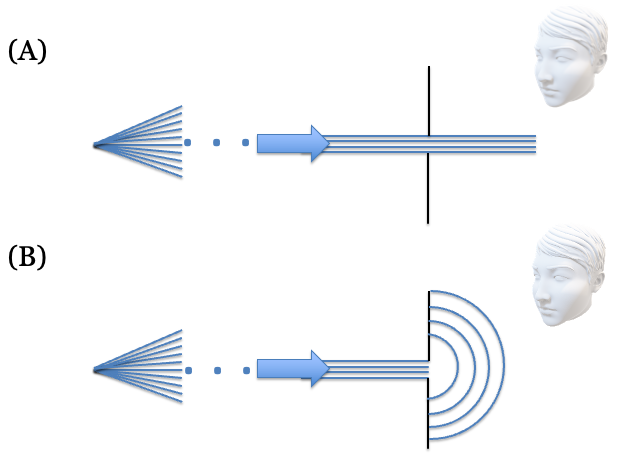
\includegraphics[width=0.8\textwidth,height=\textheight]{chapters/images/optics/06-geometric/ray-wave.png}

}

\caption{\label{fig-ray-wave}Grimaldi's experiment showing light passing
through a pinhole. According to the ray theory, the image on the screen
should be the same size as the pinhole, and an observer to the side
should see nothing. Grimaldi found that the image was often larger and
that light spread out, allowing the pinhole to be seen from the side.
Newton confirmed the experiment but continued to use the ray theory for
its practical utility, a pragmatic approach we still follow today.}

\end{figure}%

The trade-off between pinhole size and image sharpness provides a
second, compelling example of diffraction. In their classic textbook,
Jenkins and White showed a series of images of a light bulb filament
through pinholes of decreasing size (Jenkins and White (1976)). As
predicted by the ray model, reducing the pinhole size initially sharpens
the image. But beyond a certain point, further reducing the pinhole size
makes the image \emph{blurrier}, directly contradicting the ray model.
These observations demand an explanation that goes beyond geometric
optics.

\begin{figure}

\centering{

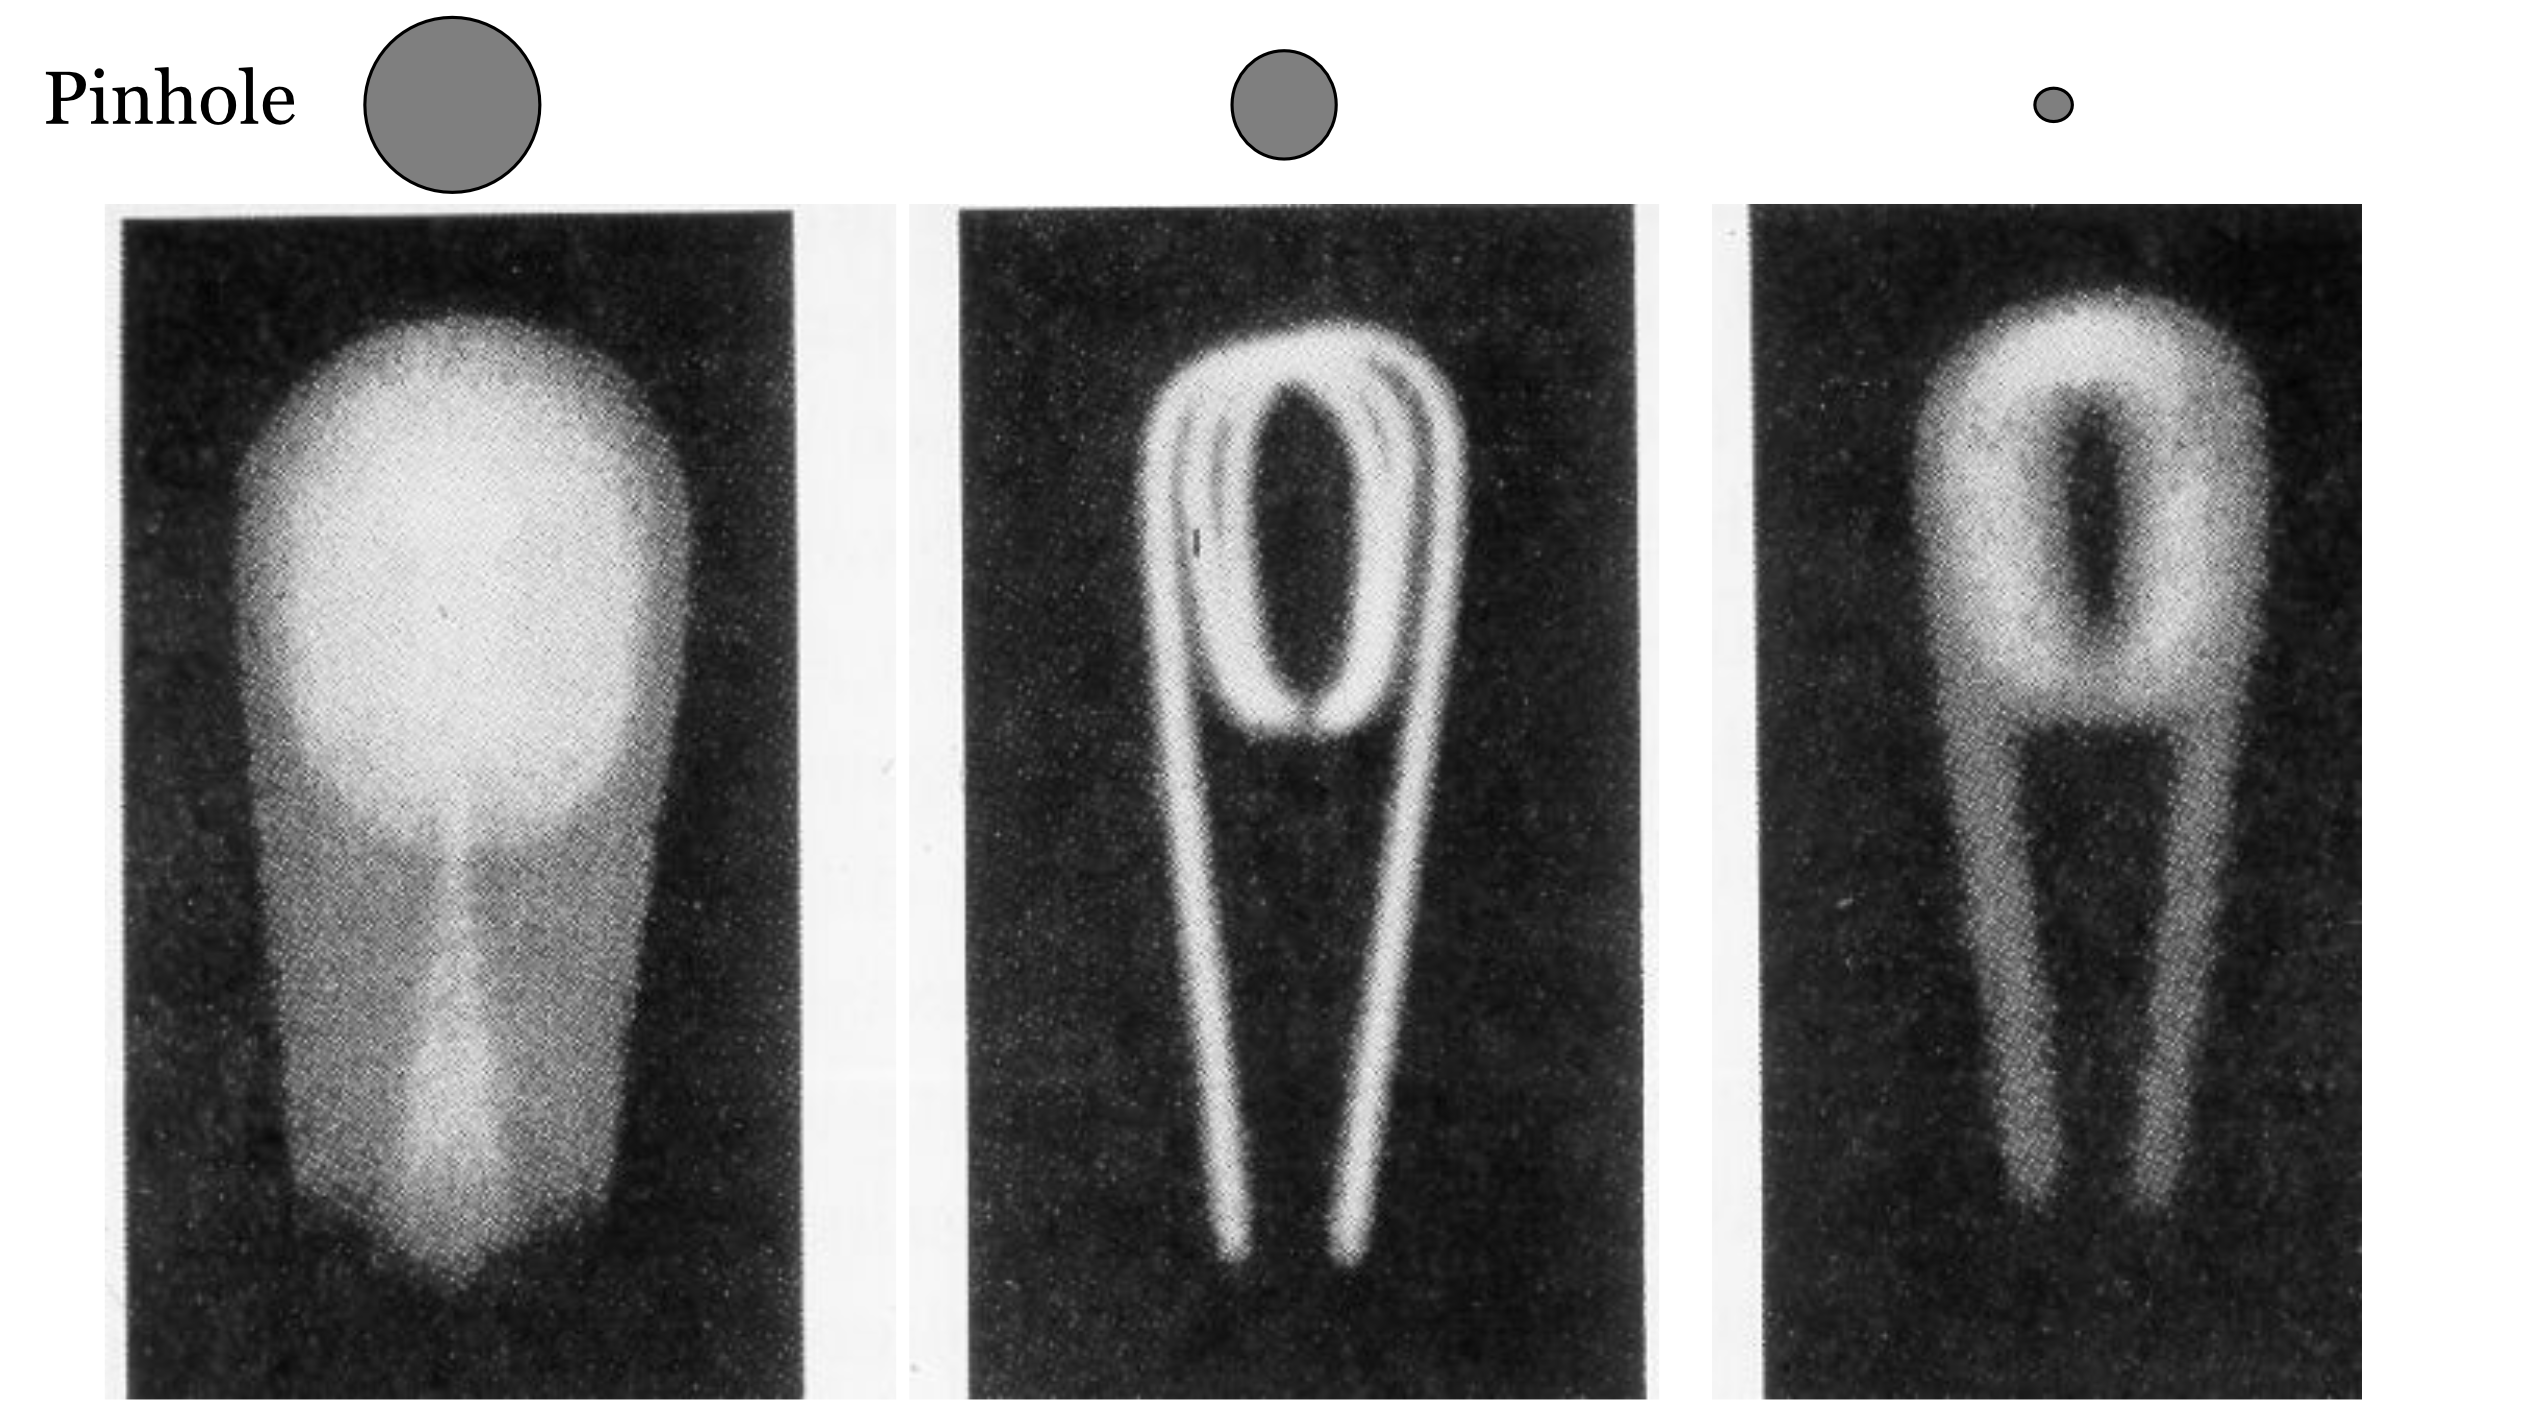
\includegraphics[width=0.7\textwidth,height=\textheight]{chapters/images/optics/06-geometric/diffraction-filaments.png}

}

\caption{\label{fig-diffraction-filaments}Images of a light bulb
filament through pinholes of decreasing size. Initially, a smaller
pinhole yields a sharper image (as predicted by geometric optics).
However, as the pinhole becomes very small, the image becomes blurrier
due to diffraction. After Jenkins and White, Jenkins and White (1976).}

\end{figure}%

\section{Huygens wave model}\label{sec-huygens-wave}

The Dutch scientist Christiaan Huygens, working at the same time as
Newton, proposed an alternative to the ray model: he modeled light as
waves expanding to fill space. In Huygens' theory, light from a point
source expands as a spherical wave. The leading edge of this expansion,
the \textbf{wavefront}, can be seen as a collection of points, each
acting as a source for a new secondary wavelet. This model successfully
predicts many phenomena, including reflection from a mirror and the
change in light's direction (refraction) as it passes from one medium to
another (Figure~\ref{fig-huygens-waves}).

\begin{figure}

\centering{

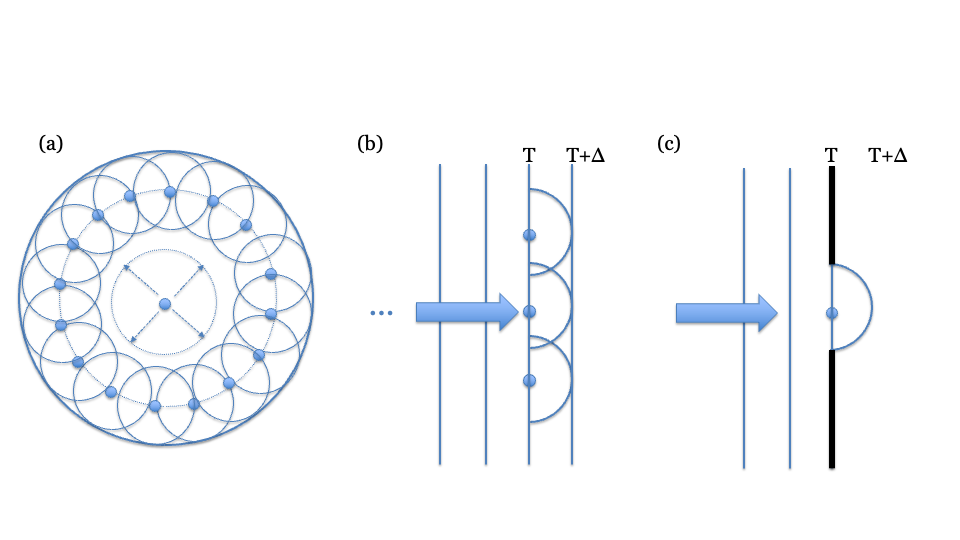
\includegraphics[width=0.8\textwidth,height=\textheight]{chapters/images/optics/06-geometric/huygens-wave.png}

}

\caption{\label{fig-huygens-waves}Light modeled as a wavefront. (A) A
point source emits a spherical wave. Each point on the expanding
wavefront acts as a source for a new secondary wavelet, and their common
tangent forms the new wavefront. (B) Far from the source, a small
section of the wavefront approximates a plane wave, which propagates
forward in the same manner. (C) When a plane wave encounters a small
aperture, only a few secondary sources pass through, revealing their
spherical nature and causing the light to spread out.}

\end{figure}%

When a plane wave travels through open space, the constructive
interference of all the secondary wavelets results in a new plane wave
that propagates straight ahead, much like an ocean wave. However, when
this wavefront passes through a small aperture or near an edge, the
aperture blocks most of the secondary sources. The few wavelets that do
pass through are revealed, causing the light to spread out spherically.

This directly explains diffraction. A very small pinhole allows only a
tiny portion of the wavefront to pass, which then propagates outward as
a nearly perfect spherical wave, allowing it to be seen from many
directions. As the aperture size increases, more of the plane wave
passes through, and the output more closely resembles a plane wave. This
wave model elegantly explains why a pinhole's effect on an image depends
so critically on its size relative to the wavelength of light.

\begin{tcolorbox}[enhanced jigsaw, bottomtitle=1mm, titlerule=0mm, arc=.35mm, colbacktitle=quarto-callout-note-color!10!white, coltitle=black, toprule=.15mm, bottomrule=.15mm, breakable, colframe=quarto-callout-note-color-frame, left=2mm, opacityback=0, colback=white, title=\textcolor{quarto-callout-note-color}{\faInfo}\hspace{0.5em}{Rays, waves and hypotheses}, opacitybacktitle=0.6, toptitle=1mm, rightrule=.15mm, leftrule=.75mm]

Although the ray and wave theories were proposed at about the same time,
Newton's 1704 framing of light as rays was widely accepted for roughly a
century. Widespread recognition of the accuracy of Huygen's wave theory
was delayed until Thomas Young's 1804 demonstration of the interference
pattern created by light from two coherent, nearby sources. I find it
interesting to learn about the
\href{../resources/optics-diffraction.html}{the history of these
ideas.}.

I have worked in fields where scientists rely mainly on hypothesis
testing: they perform experiments to see if a theory is provably wrong.
Surely Newton's theory of light as a ray is provably wrong, and it was
so proved more than 300 years ago! And yet, we use rays to describe
light routinely. This is because in many cases the ray theory is an
excellent approximation, and we use it as a simple way to reason about
radiation - approximately.

This is a very pragmatic approach, which is deeply embedded in the mind
of many scientists and engineers: Use the tool that is accurate enough
for the problem at hand. Approach your problem with a toolbox of
methods, and choose the one that gets the job done. In this spirit, the
phrase `all models are wrong, some are useful', Box (1976) is widely
quoted in many engineering disciplines. In these fields hypotheses that
are useful are included in the toolbox. It is essential to understand
the scope over which the tool can be reasonably relied upon.

\end{tcolorbox}

\section{Double slit experiments}\label{double-slit-experiments}

Grimaldi's observations documenting how light spreads out after passing
the edge of an obstacle or through a narrow slit, are easily
reproducible and important. Huygens put forward a genuine wave theory of
light. His principle of secondary wavelets elegantly explained
reflection and refraction, and even hinted at diffraction (Huygens
(1690)). It is surprising to me that Newton felt he could promote a ray
theory of light despite these prior observations and theory. It was
fascinating to learn that Newton and Huygens directly confronted one
another on both optics and gravity (Shapiro (1989)). Perhaps because
Newton was remarkable in so many ways, his voice dominated the
scientific scene for decades.

Even though Huygens theory did account for many important phenomena; to
me the simple observation in Figure~\ref{fig-ray-wave} decisively
demonstrates the necessity of a theory that allows for waves.
Nonetheless, it wasn't until Thomas Young presented his famous
double-slit experiments to the Royal Society in 1801--1803 that Newton's
hold on the field began to loosen (Young (1804b)). This paper was a
crucial step in the shift of the scientific consensus towards the wave
theory of light. The ability to see the interference fringes provided
quantitative, unmistakable proof of the value of the wave theory. Only
waves, not particles, could add and cancel in this way and made the
phenomenon hard to ignore. Young -and many others- considered- the
demonstration of interference to be decisive\footnote{In making some
  experiments on the fringes of colours accompanying shadows, I have
  found so simple and so demonstrative a proof of the general law of the
  interference of two portions of light, which I have already
  endeavoured to establish, that I think it right to lay before the
  Royal Society, a short statement of the facts which appear to me so
  decisive (Young (1804b)).}.

The experiment requires some precision, but it is fairly straightforward
to instrument (Figure~\ref{fig-double-slit}). One begins with a
collimated beam arriving at a small aperture (part A). The light passing
through the aperture serves as a coherent light source. It is allowed to
transport forward to a second surface that has two narrow slits
separated by some small distance. It is now the turn of these two slits
to provide separated coherent light sources. When we observe the image
formed by the double slits on a surface, the image is a striped pattern.
As Young explained and drew in his original paper (part B), this is what
one might expect of the two slits are both emitting waves at the same
frequency.

\begin{figure}

\centering{

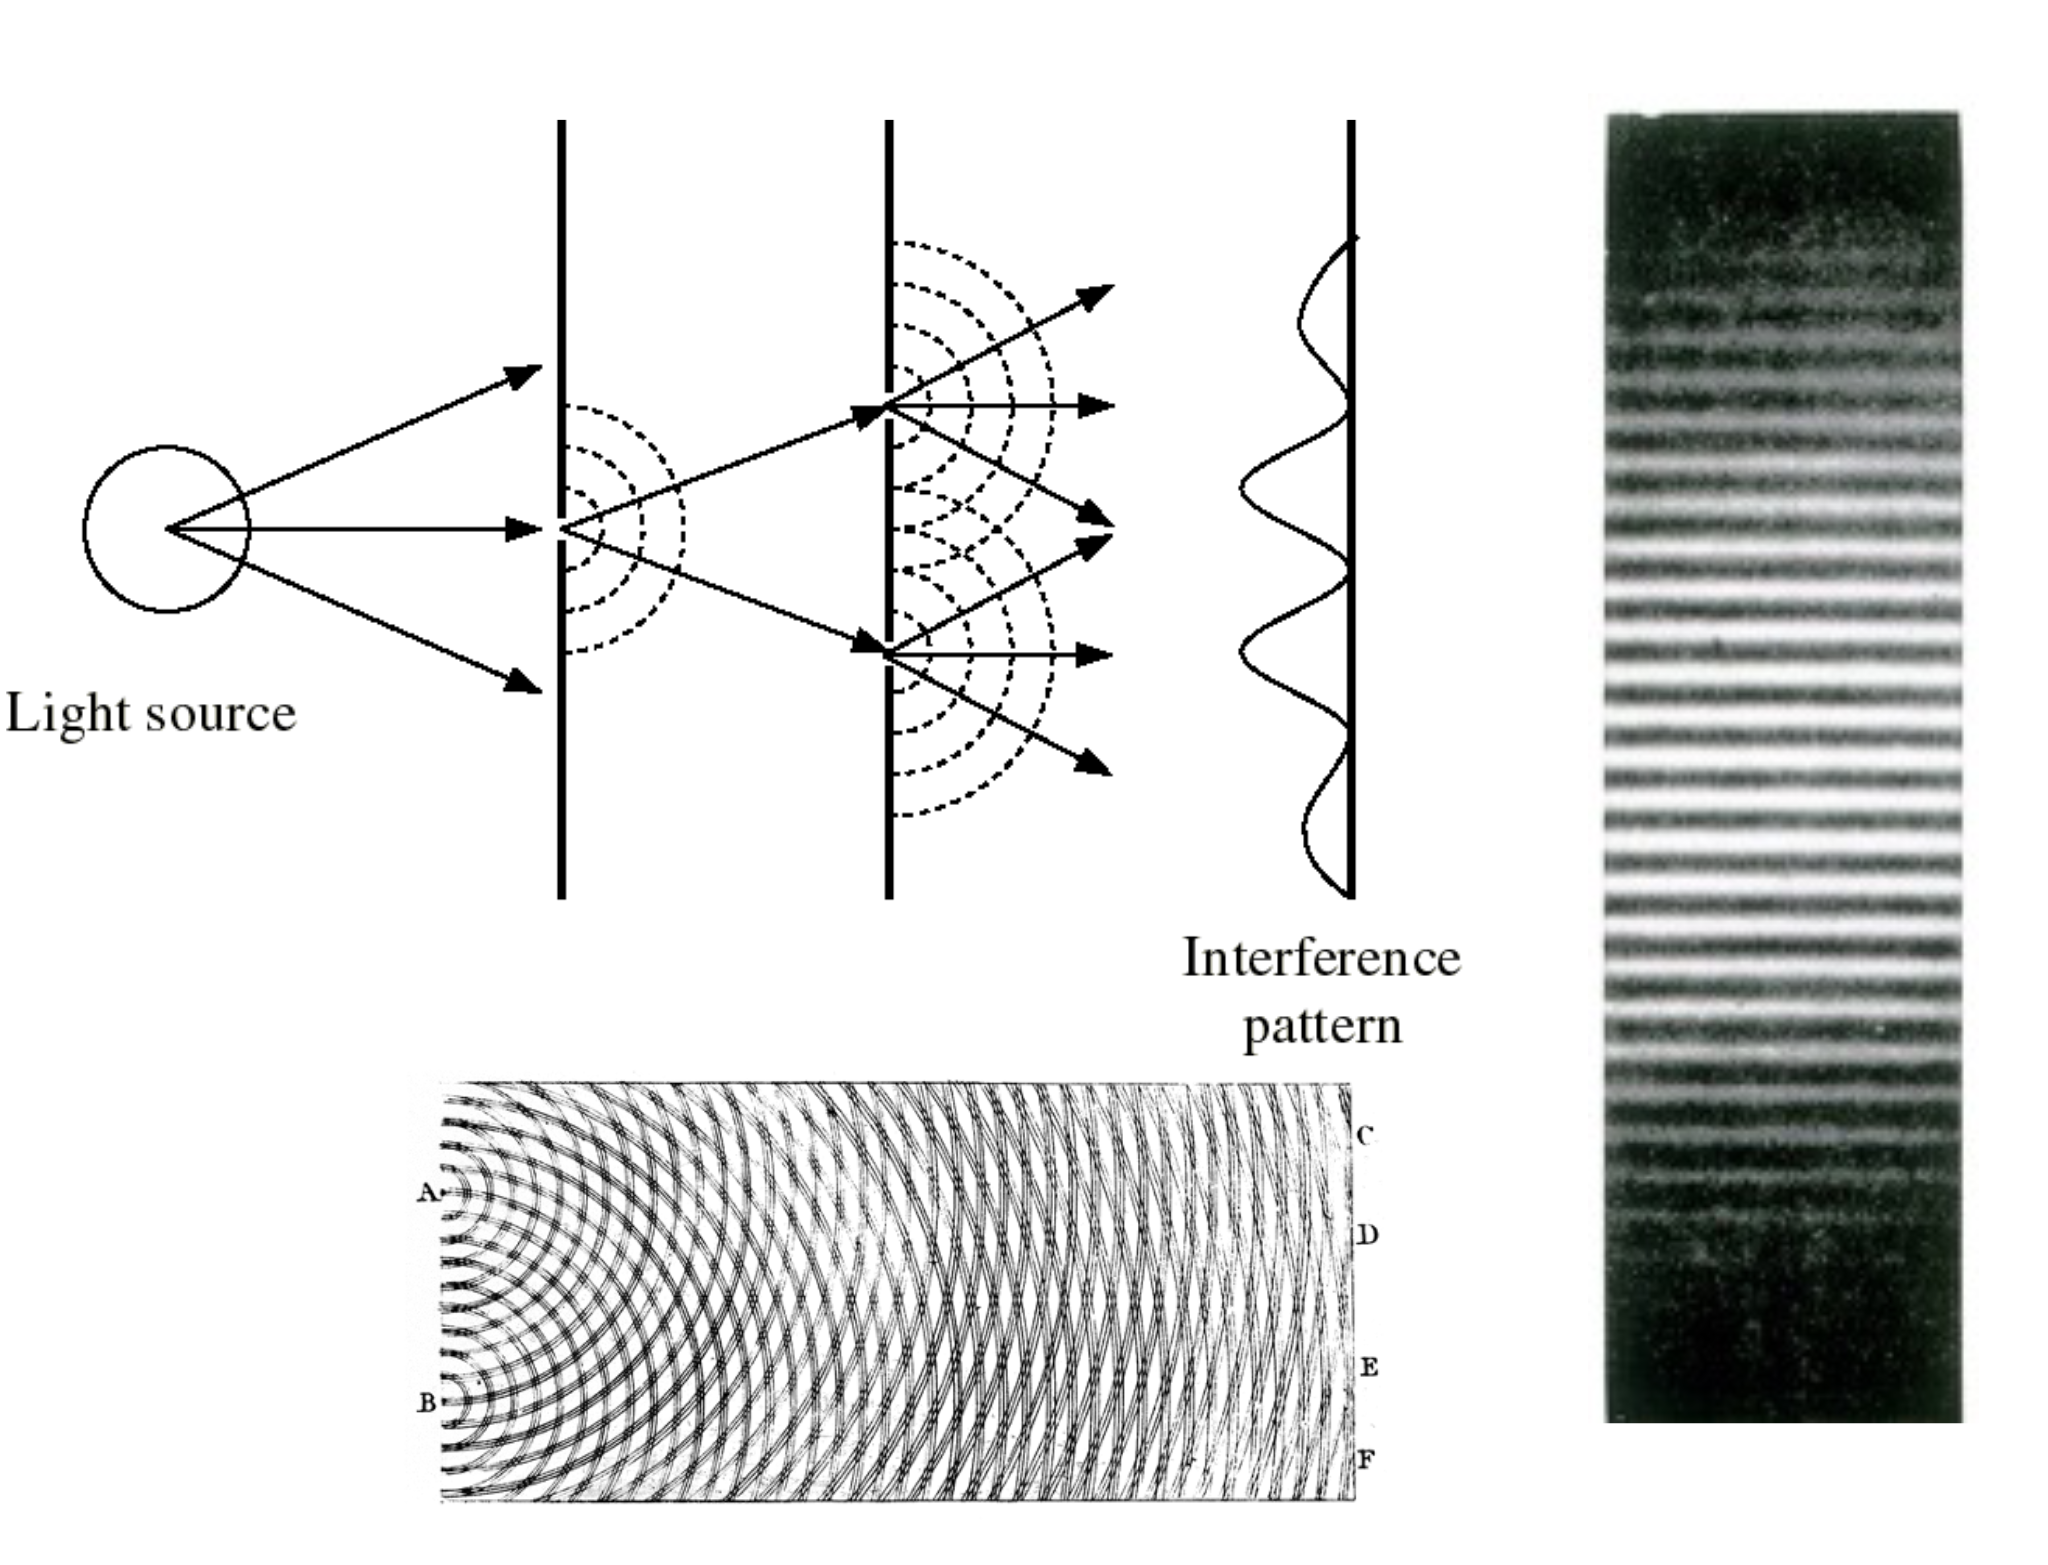
\includegraphics[width=0.8\textwidth,height=\textheight]{chapters/images/optics/06-geometric/double-slit.png}

}

\caption{\label{fig-double-slit}Thomas Young's double slit experiment.
Young's drawing is available from
\href{https://en.wikipedia.org/wiki/Diffraction\#/media/File:Young_Diffraction.png}{Wikipedia}}

\end{figure}%

Even after Young's presentations to the Royal Society, the wave theory
met resistance. The loudest was from Henry Brougham who made personal
attacks on Young\footnote{Henry Brougham was a particularly fierce
  critique of Young's entire research program and an ardent defender of
  Newton's work. His strongest attacks were against Young's important
  -and accurate!- observations about human color vision. More on that,
  including Young's response (Young (1804a)) in Chapter~\ref{sec-human}.}.
But serious thinkers also wondered whether a wave theory could be right.
What was the medium that supported the waves? Huygens referred to it,
but the so-called `ether' had not been measured\footnote{``Now there is
  no doubt at all that light also comes from the luminous body to our
  eyes by some movement impressed on the matter which is between the
  two.''---Christiaan Huygens}. And if the waves were propagating
through a medium, wouldn't inhomogeneities cause them to deviate from
straight lines?

A particularly important event that turned the tide occurred a decade
later, when Augustin-Jean Fresnel supplied the mathematics of
diffraction and interference. This was a famous event in the history of
physics. In 1818, Fresnel submitted his wave theory to a competition
sponsored by the French Academy of Sciences. One of the judges,
Siméon-Denis Poisson, was a staunch supporter of Newton's particle
theory and sought to disprove Fresnel's work. Using Fresnel's own
equations, Poisson calculated that if a circular obstacle were
illuminated by a point source of light, a bright spot should appear in
the very center of the shadow. Poisson presented this as a
\emph{reductio ad absurdum}---an absurd conclusion that surely proved
the wave theory was wrong.

However, the head of the committee, François Arago, decided to perform
the experiment. To the astonishment of many, Arago observed the bright
spot exactly as predicted. This dramatic confirmation of a
counter-intuitive prediction was a decisive victory for the wave theory.
The spot is now ironically known as \textbf{Poisson's spot} (or
sometimes Arago's spot). This work ended the dominance of the
corpuscular theory for some time. It was to return with Einstein's work,
which I explain in Chapter~\ref{sec-sensors-photons-electrons}.

\begin{tcolorbox}[enhanced jigsaw, bottomtitle=1mm, titlerule=0mm, arc=.35mm, colbacktitle=quarto-callout-note-color!10!white, coltitle=black, toprule=.15mm, bottomrule=.15mm, breakable, colframe=quarto-callout-note-color-frame, left=2mm, opacityback=0, colback=white, title=\textcolor{quarto-callout-note-color}{\faInfo}\hspace{0.5em}{A modern double-slit experiment}, opacitybacktitle=0.6, toptitle=1mm, rightrule=.15mm, leftrule=.75mm]

I was delighted to see the fundamental principle of the double-slit
experiment return in my Inbox while writing this book. The core idea of
the experiment is to measure the superposition of two signals. Even as
technology has scaled, scientists continue to use this principle to
investigate and characterize the properties of electromagnetic
radiation.

\begin{figure}[H]

\centering{

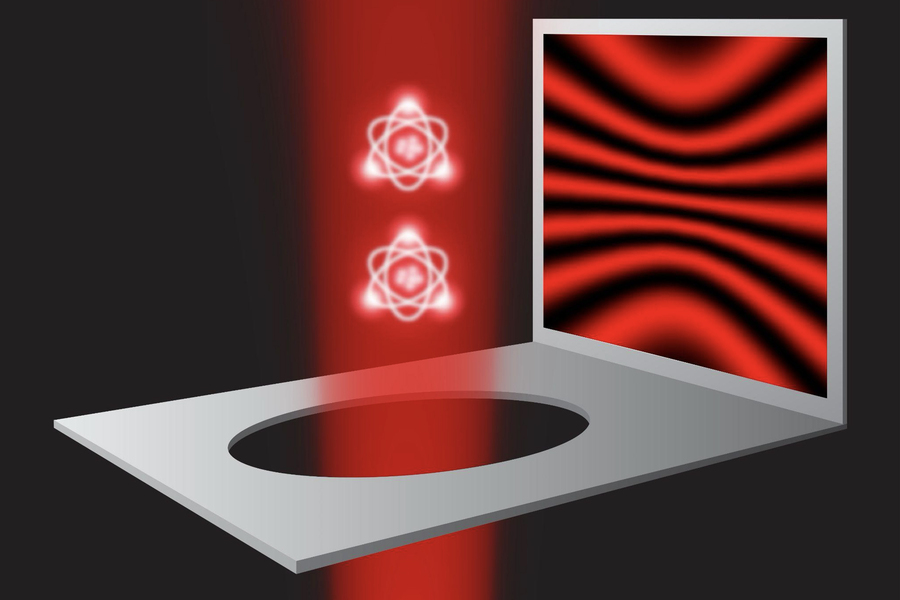
\includegraphics[width=0.6\textwidth,height=\textheight]{chapters/images/optics/06-geometric/double-slit-atoms.png}

}

\caption{\label{fig-double-slit-atoms}Atoms and the double-slit. The
image shows two single atoms floating in a vacuum chamber are
illuminated by a laser beam and act as the two slits. The interference
of the scattered light is recorded with a highly sensitive camera
depicted as a screen. Incoherent light appears as background and implies
that the photon has acted as a particle passing only through one slit.
(Courtesy: Wolfgang Ketterle, Vitaly Fedoseev, Hanzhen Lin, Yu-Kun Lu,
Yoo Kyung Lee and Jiahao Lyu)}

\end{figure}%

Here is a link to see the
\href{https://physicsworld.com/a/famous-double-slit-experiment-gets-its-cleanest-test-yet/?utm_source=Live+Audience&utm_campaign=01bdf7753f-nature-briefing-daily-20250827&utm_medium=email&utm_term=0_b27a691814-01bdf7753f-49658492}{article
in Physics World.}

\end{tcolorbox}

\section{Pinhole size or diffraction: which blurs
more?}\label{sec-airy-pattern}

From these simple considerations, we have seen that the image is blurred
by two effects: the pinhole size and diffraction. Increasing the pinhole
would create a larger spot on the wall, but decreasing the pinhole size
reveals the spherical nature of the wavefront and also increases the
size of the spot on the wall. We can compare the size of these two
effects numerically.

\begin{figure}

\sidecaption{\label{fig-blur-comparison}The Airy pattern of a pinhole
camera.}

\centering{

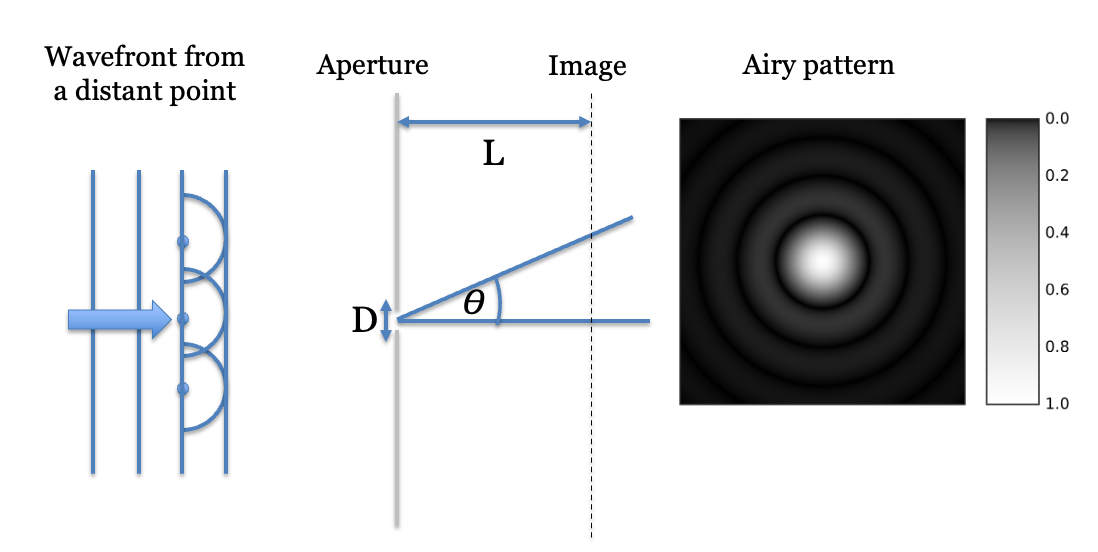
\includegraphics[width=0.8\textwidth,height=\textheight]{chapters/images/optics/06-geometric/blur-comparison.png}

}

\end{figure}%

First, consider what we expect from the ray model. If the pinhole
diameter is \(D\), a far-away point on the main axis will produce a
blurred spot in the image of size \(D\). Also, the pinhole-blur
predicted by the ray model is the same no matter how far the image plane
is from the pinhole.

Second, consider the light pattern we expect for a plane wave passing
through a pinhole aperture. This pattern can be calculated using a
formula derived by the astronomer, George B. Airy (Airy 1835) and is
shown in Figure~\ref{fig-blur-comparison}. The Airy pattern has a
central bright spot (the Airy disk), which is surrounded by a series of
concentric rings. The size of the pattern depends on the wavelength of
the light \(\lambda\), the diameter of the pinhole \(D\). Unlike the ray
model, for the diffraction case the rays are expanding so that the
distance \(L\) from the pinhole to the image plane matters. The image is
radially symmetric with a bright spot in the center, surrounded by a set
of concentric rings of decreasing intensity. The Airy disk contains
about 85\% of the total energy. The mathematical notation for the Airy
pattern is a bit complex, but the diameter of the Airy disk, \(d\), has
a simple formula

\begin{equation}\phantomsection\label{eq-airy1}{
d = 2.44~L~(\lambda / D)
}\end{equation}

Suppose we calculate the size of the diffraction diameter when the image
plane is 1 m away, so \(L=1\), and for a wavelength of light is 550 nm.
Suppose the pinhole diameter is \(D = 10^{-4} m\). The diameter of the
Airy disk, \(d\), will be

\begin{equation}\phantomsection\label{eq-airydisk1}{
d = 2.44 \times (1 m) (550 \times 10^{-9} m )/ 1 \times 10^{-4}m) = 0.0134 m
}\end{equation}

The diffraction spread exceeds the pinhole spread when \(d\) exceeds
\(D\). We do the calculation for different assumptions about the
distance to the image plane \href{./code/fise_diffraction.html}{ISETCam
script}. As an example, we find that when the distance to the image
plane is \(L = 1m\), the pinhole blur is larger than the diffraction
blur for a pinhole diameter of about \(1 mm\). When the image plane
distance, \(L\), is closer, say \(10 mm\), the pinhole blur exceeds the
diffraction blur when the diameter is \(100 \mu\).

\begin{tcolorbox}[enhanced jigsaw, bottomtitle=1mm, titlerule=0mm, arc=.35mm, colbacktitle=quarto-callout-note-color!10!white, coltitle=black, toprule=.15mm, bottomrule=.15mm, breakable, colframe=quarto-callout-note-color-frame, left=2mm, opacityback=0, colback=white, title=\textcolor{quarto-callout-note-color}{\faInfo}\hspace{0.5em}{The diameter of the diffraction point spread}, opacitybacktitle=0.6, toptitle=1mm, rightrule=.15mm, leftrule=.75mm]

In a paper entitled ``On the Diffraction of an Object-glass with
Circular Aperture'', George Airy provided the mathematical description
of the diffraction pattern (Airy 1835). A modern derivation of the full
point spread function for both the circular aperture and other shapes is
in Goodman (2022) (pages 88-94). The computation is implemented and
frequently used in ISETCam. It is explained
\href{https://htmlpreview.github.io/?https://github.com/ISET/isetcam/blob/main/tutorials/optics/t_opticsAiryDisk.html}{in
this tutorial}.

In the main text, we expressed the formula for a particular distance
from the pinhole to an image plane. For a pinhole, the formula is
usually given in terms of the angle of the bundle of rays emerging from
the pinhole.

\[sin(\theta) = 1.22 \lambda / D\]

When the angle is small, \(\theta < 10 \deg\), the formula is very
accurately approximated as

\[
\theta = 1.22 \lambda / D
\]

The size of the spot on the image plane depends on the distance how far
away the pinhole is from the pinhole, as you can see in
Equation~\ref{eq-airy2}. In Chapter~\ref{sec-optics-thinlens} we provide
a formula for the Airy disk size for ideal lenses.

\end{tcolorbox}

\section{Point spread functions}\label{sec-pointspread}

Throughout this section, we have discussed how a single point of light
is imaged by an optical system. The resulting image is called the
\textbf{point spread function (PSF)}, and it is a fundamental measure of
optical performance. The Airy pattern, for example, is the PSF produced
by a circular aperture due to diffraction. We will encounter other types
of PSFs when we analyze optical systems using linear systems theory
(Chapter~\ref{sec-optics-linear-space}).

It is important to note that most optical systems, including lenses, do
not have a single, fixed PSF. The PSF can vary depending on the distance
to the point source and its position in the field of view. For systems
with circular symmetry, the position is often described by the
\textbf{field height}, which is the angle between the optical axis and
the point's location.

Even in pinhole imaging, the PSF is not unique. There are two main
diffraction regimes to consider. When the point source is far from the
pinhole, the incoming wavefront is essentially planar, and the resulting
diffraction pattern is described by \textbf{Fraunhofer diffraction} (or
\href{https://en.wikipedia.org/wiki/Fraunhofer_diffraction}{far-field
diffraction}). In this case, the Airy pattern accurately describes the
PSF.

When the point source is close to the pinhole, the wavefront is curved
(spherical), and the diffraction pattern changes. This situation is
described by \textbf{Fresnel diffraction} (or
\href{https://en.wikipedia.org/wiki/Fresnel_diffraction}{near-field
diffraction}). Here, the PSF depends on the distance from the source to
the aperture.

We will explore the role of the PSF in lens simulation,
characterization, and computational imaging methods in
Chapter~\ref{sec-optics-linear-space} and the following chapters.

\section{Pinhole shapes and PSFs}\label{pinhole-shapes-and-psfs}

To this point we have only considered circular pinholes. These are
important because many apertures, including the human pupil, are close
to circular. Also, many camera systems use approximately circular
apertures. The nice feature of circular apertures is that rotating the
camera (or our head) leaves the optical impact of the aperture
unchanged. When the point spread function is circularly symmetric, as
for the Airy pattern, we can describe it using only the radial distance
from the PSF center.

There are cases in nature -and industry- of non-circular apertures, and
these point spread functions must be described as two-dimensional
images. In the following sections I introduce an ISETCam script that
calculates the diffraction-limited PSF for some non-circular
diffraction-limited apertures.

\subsection{Rectangular pinholes}\label{rectangular-pinholes}

The script
\href{../code/02Optics/fise_oiAperturemlx.html}{fise\_oiAperture}
illustrates how to calculate the PSF for a rectangular aperture in
ISETCam. An image computed using the PSF from a diffraction limited
rectangular pinhole, and the PSF for that pinhole, are shown in
Figure~\ref{fig-pinhole-rectangle}. The images illustrate a case for the
rectangular aperture is three times wider (x) than high (y). The larger
vertical height causes less blur in the y-direction, making the image
sharper for the horizontal stripes.

\begin{figure}

\centering{

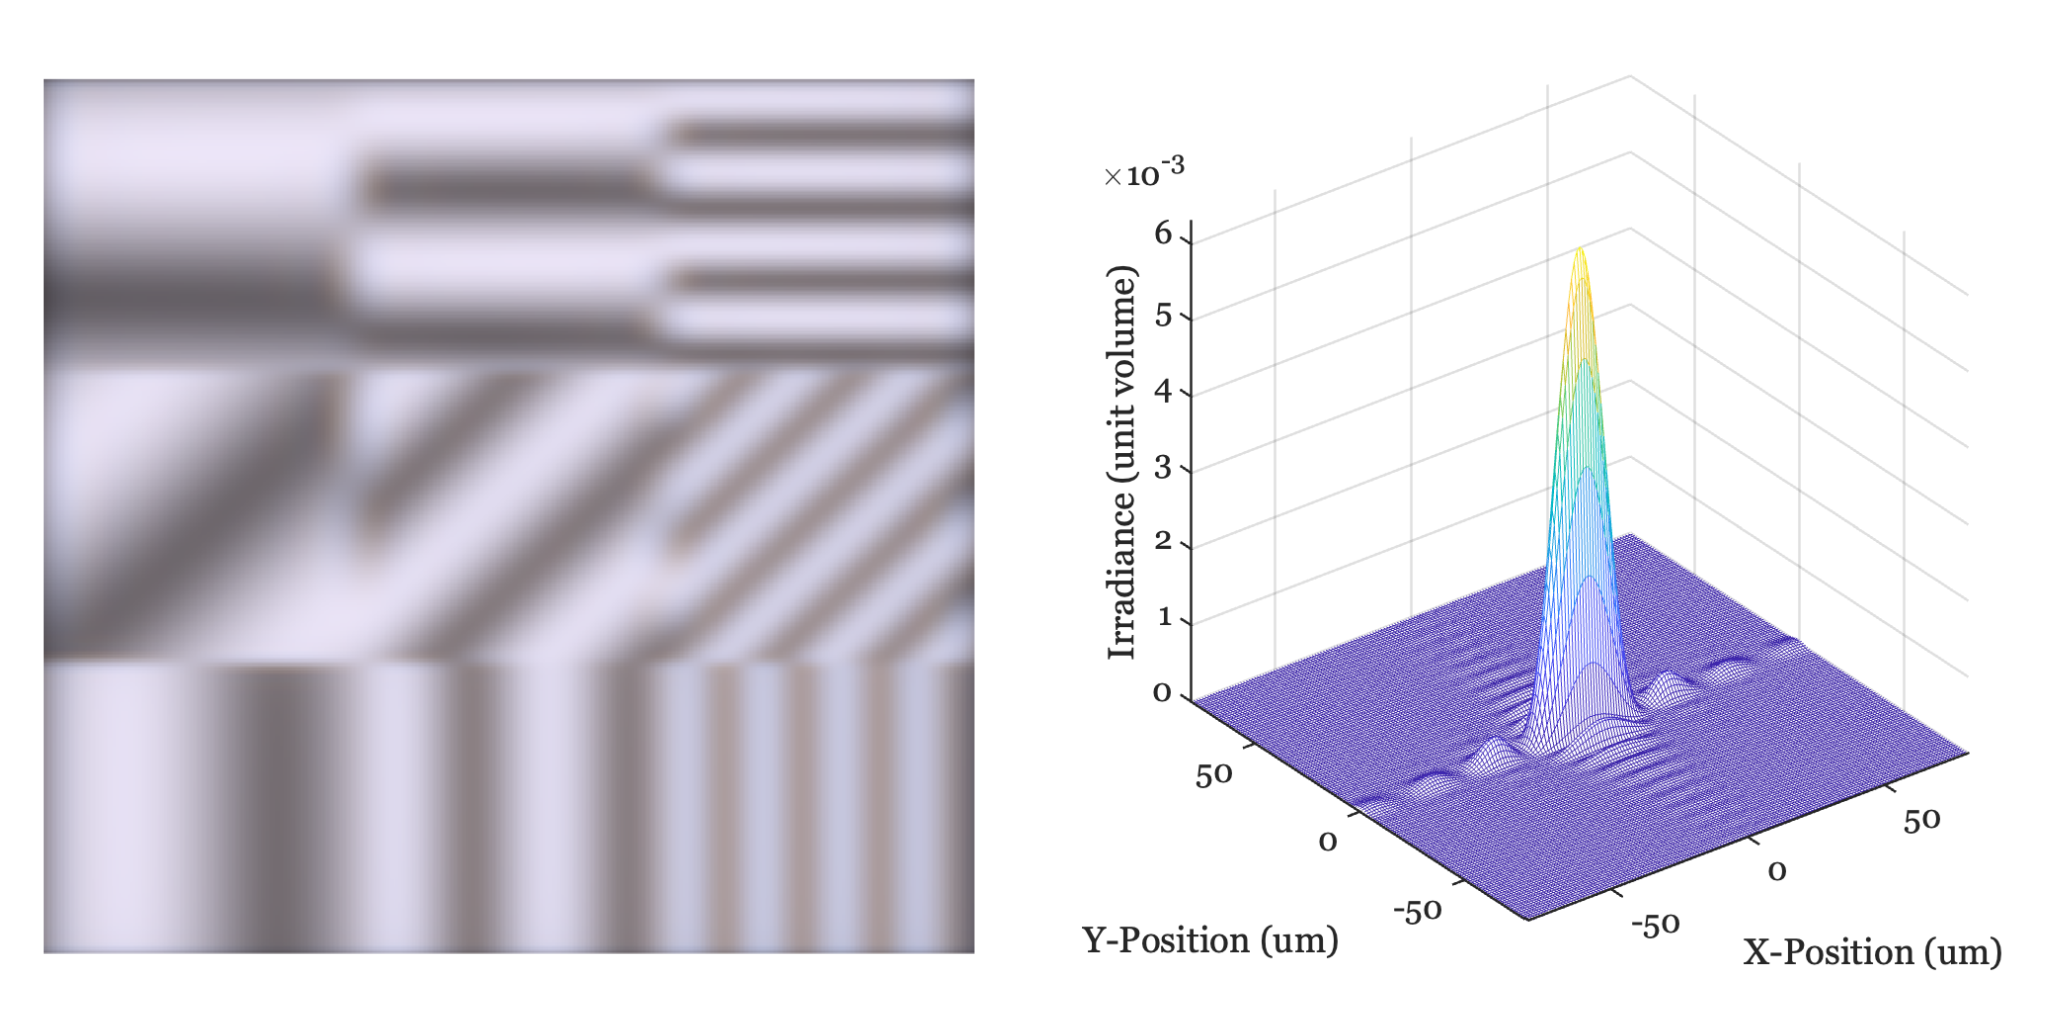
\includegraphics[width=0.8\textwidth,height=\textheight]{chapters/images/optics/06-geometric/pinhole-rectangle-both.png}

}

\caption{\label{fig-pinhole-rectangle}Simulating a diffraction-limited
rectangular pinhole that is 3x higher than wide. The test pattern has
spatial frequency increasing from left to right, and orientation varying
up to down. The horizontal lines retain their contrast as frequency
increases; the vertical lines lose theirs. The PSF (550 nm) for the
rectangular aperture is plotted on the right. See
\href{../code/02Optics/fise_oiAperturemlx.html}{fise\_oiAperture}.}

\end{figure}%

There is a formula for the rectangular diffraction-limited PSF, given in
terms of distance on the sensor surface.

\[
\text{PSF}(x',y') \;\propto\;
\left[\operatorname{sinc}\!\left(\frac{\pi a}{\lambda f}\,x'\right)\right]^2
\;\left[\operatorname{sinc}\!\left(\frac{\pi b}{\lambda f}\,y'\right)\right]^2,
\]

where \(a\) and \(b\) are the aperture widths in the \(x\) and \(y\)
directions, \(f\) is the focal length, and \(\lambda\) is the
wavelength. We define \(\operatorname{sinc}(u) = \tfrac{\sin(u)}{u}\).

In the script, you will see that I didn't use the formula directly.
Rather, I simply defined the shape of the aperture and ran a
calculation. In Chapter~\ref{sec-optics-wavefront} I will explain that
calculation. Being able to numerically compute with the wavefront means
we can find the PSF for many different shapes.

\begin{tcolorbox}[enhanced jigsaw, bottomtitle=1mm, titlerule=0mm, arc=.35mm, colbacktitle=quarto-callout-note-color!10!white, coltitle=black, toprule=.15mm, bottomrule=.15mm, breakable, colframe=quarto-callout-note-color-frame, left=2mm, opacityback=0, colback=white, title=\textcolor{quarto-callout-note-color}{\faInfo}\hspace{0.5em}{Animal pupil shapes.}, opacitybacktitle=0.6, toptitle=1mm, rightrule=.15mm, leftrule=.75mm]

Approximately rectangular pupils are fairly common in biology, as well,
and the pupil shape is associated with how they live their lives (Banks
et al. (2015)). Vertically elongated pupils are associated with ambush
predators that are active both day and night. So beware! Horizontally
elongated pupils are more likely to be found in prey, who also have
laterally placed eyes that helps them look all around.

\begin{figure}[H]

\centering{

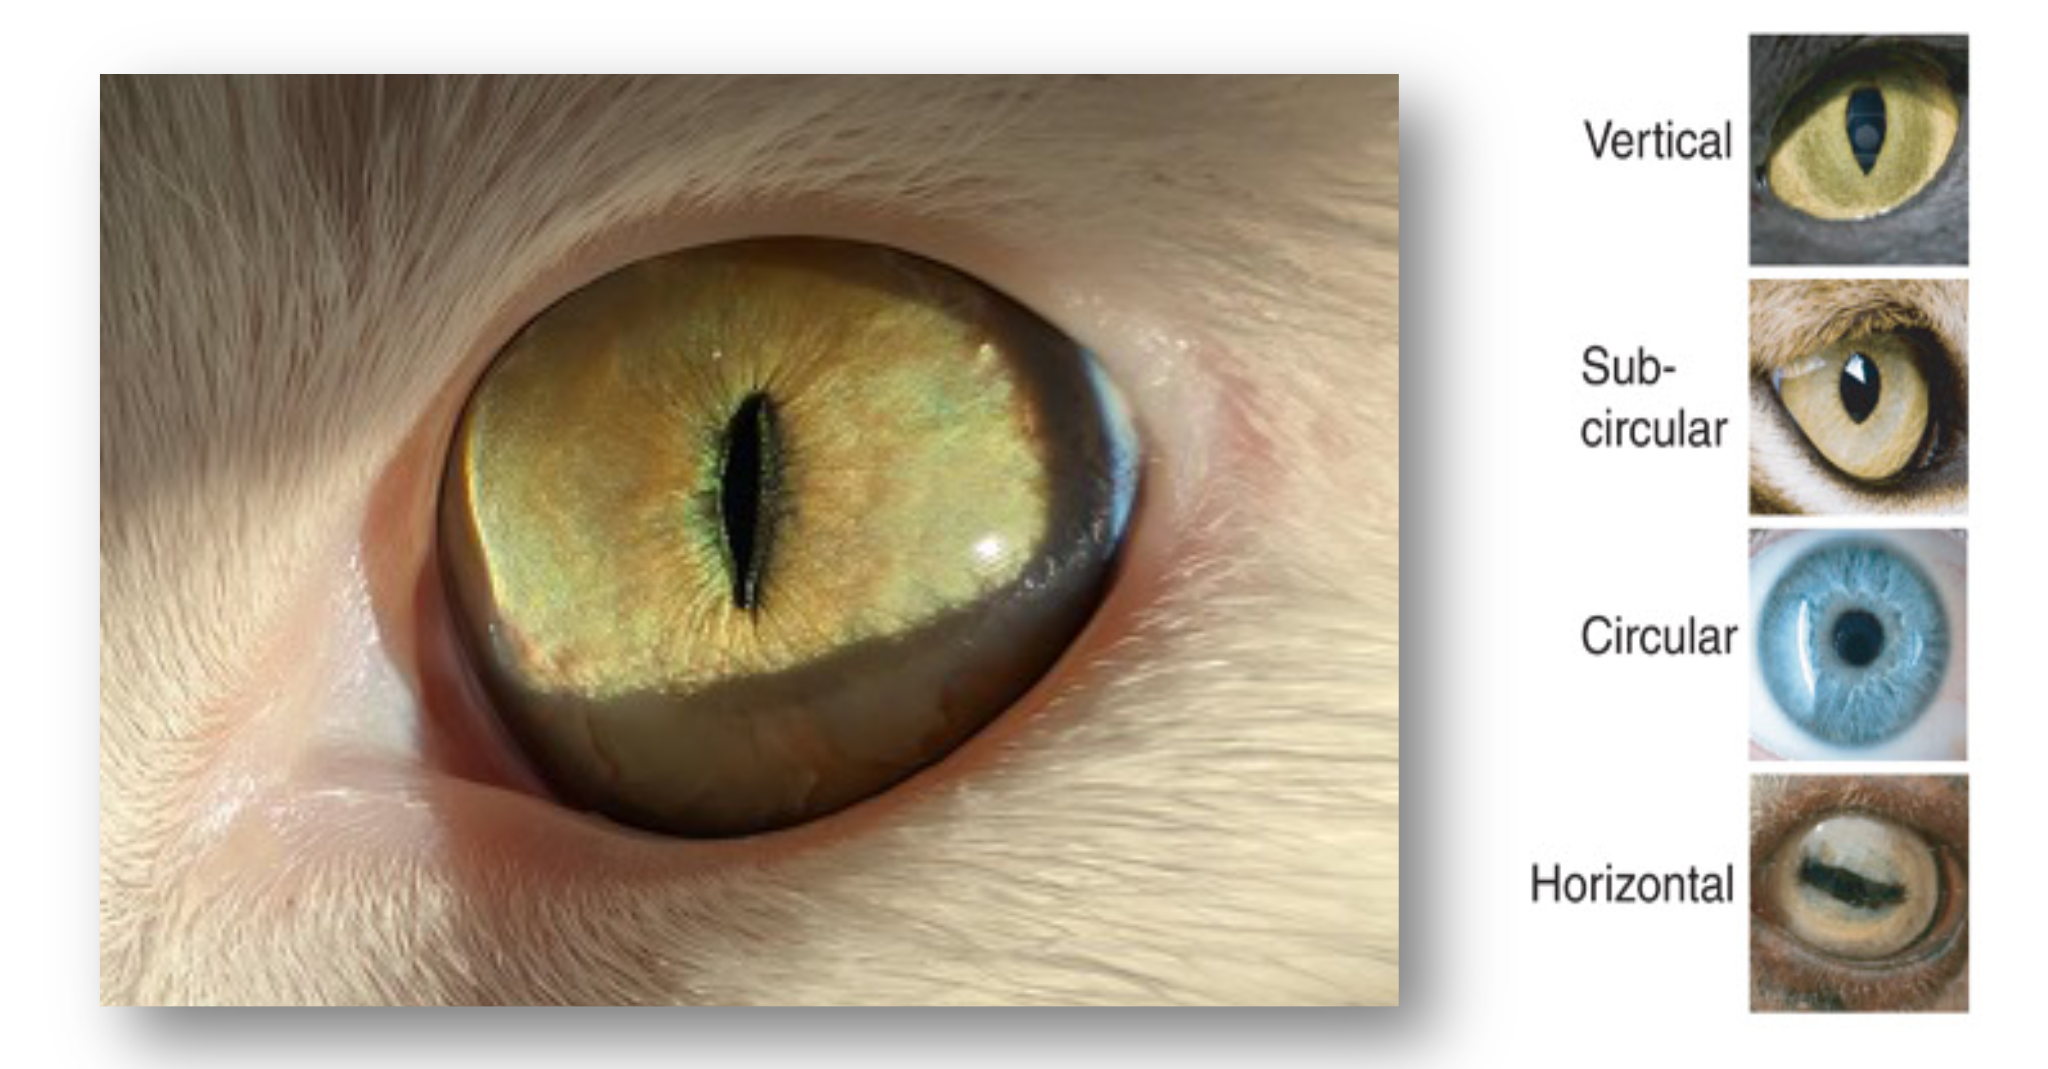
\includegraphics[width=0.6\textwidth,height=\textheight]{chapters/images/optics/06-geometric/catpupil.png}

}

\caption{\label{fig-cat-pupil}The cat has a vertical pupil - appropriate
for a killing machine. There are many, many images of the cat pupil on
the web. The cat is capable of closing its pupil nearly completely. The
images on the right are examples provided by Banks et al. (2015).}

\end{figure}%

\end{tcolorbox}

\subsection{Regular polygons}\label{regular-polygons}

Classic cameras with mechanical shutters often had regular polygon
shapes (left) or the interesting `leaf' pattern at the right. These
apertures introduce structure into the PSF that differs from a
circularly symmetric aperture.

\begin{figure}

\centering{

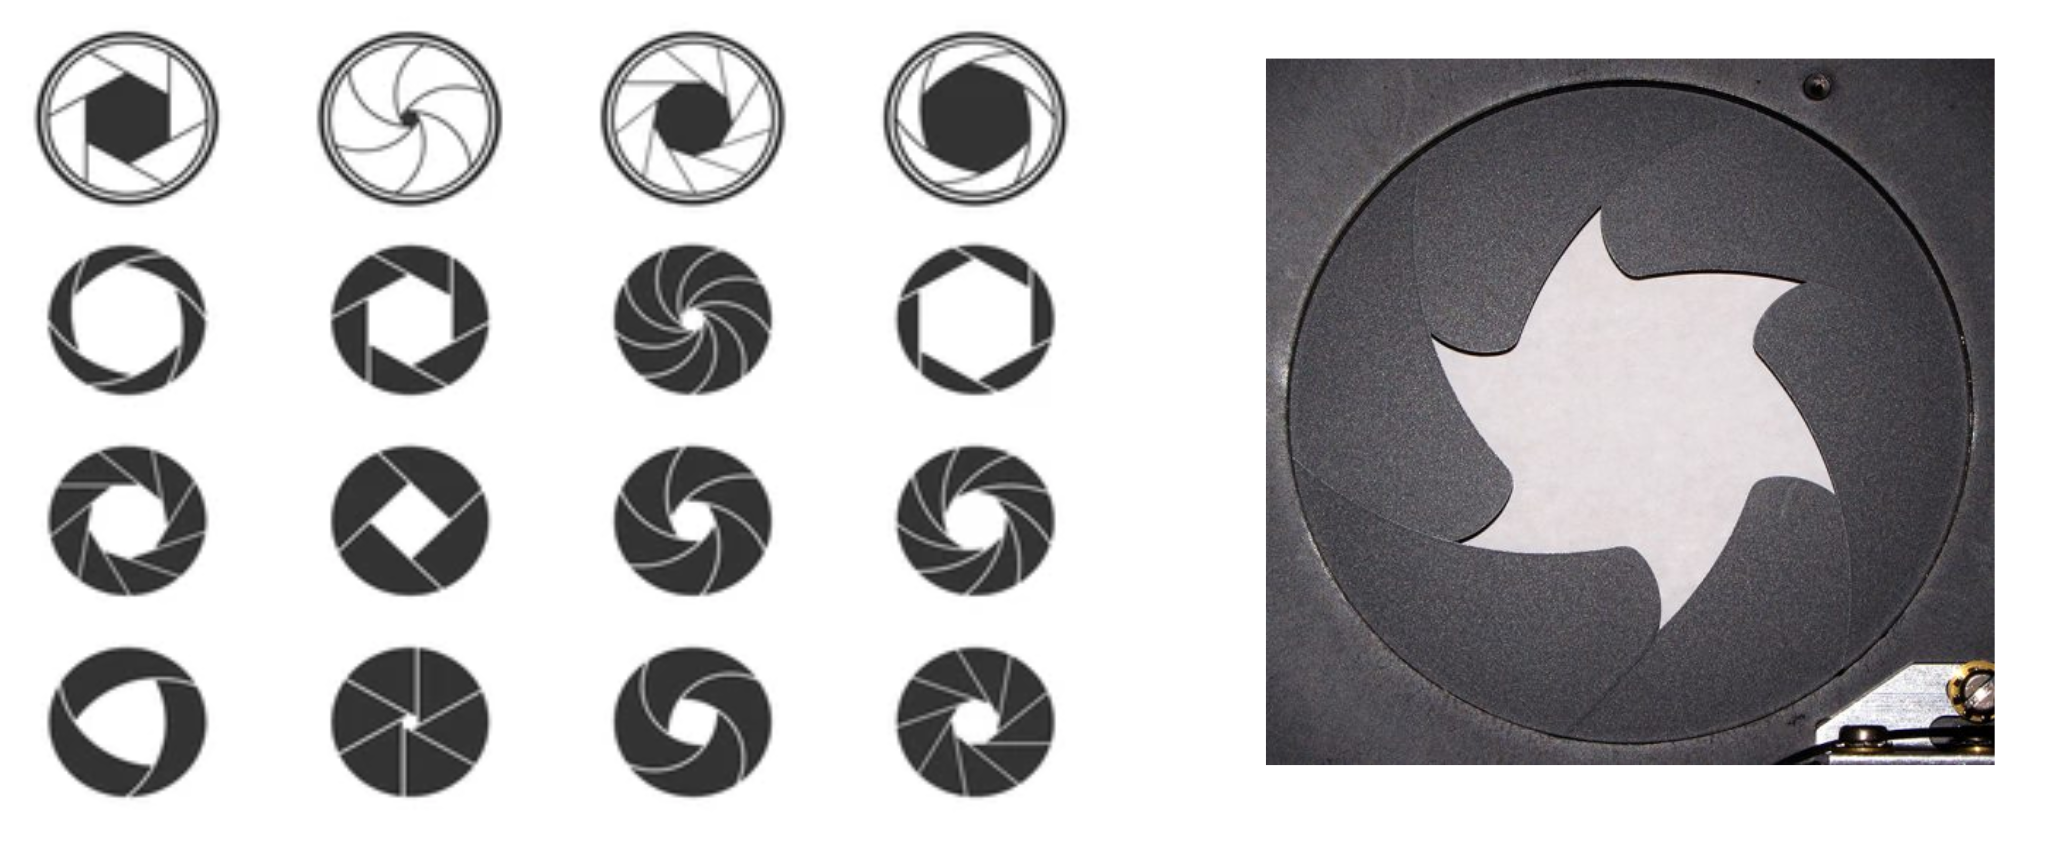
\includegraphics[width=0.6\textwidth,height=\textheight]{chapters/images/optics/06-geometric/mechanical-shutters.png}

}

\caption{\label{fig-pinhole-polygon}A sampling of mechanical shutter
shapes. The array on the left are different regular polygons. The one on
the right is called a `leaf' shutter. I have wanted to simulate its PSF,
but I haven't gotten around to it. Let me know if you try. You might
start with the script described above, and introduce the aperture shape
from an image. Or start with the image and define a mathematical
function for the shape. You can see why I never did it. I just can't
choose.}

\end{figure}%

The impact of the regular polygon shape is quite visible in high dynamic
range (HDR) scenes that include light sources. The script
\href{../code/02Optics/fise_oiAperturemlx.html}{fise\_oiAperture}
simulates an HDR scene, superimposing some very bright light sources on
the background image. These apertures produce the flare pattern that one
often sees in professional productions, including movies and sports
shows. The three images show the flare pattern for polygons with
different numbers of sides.

\begin{figure}

\centering{

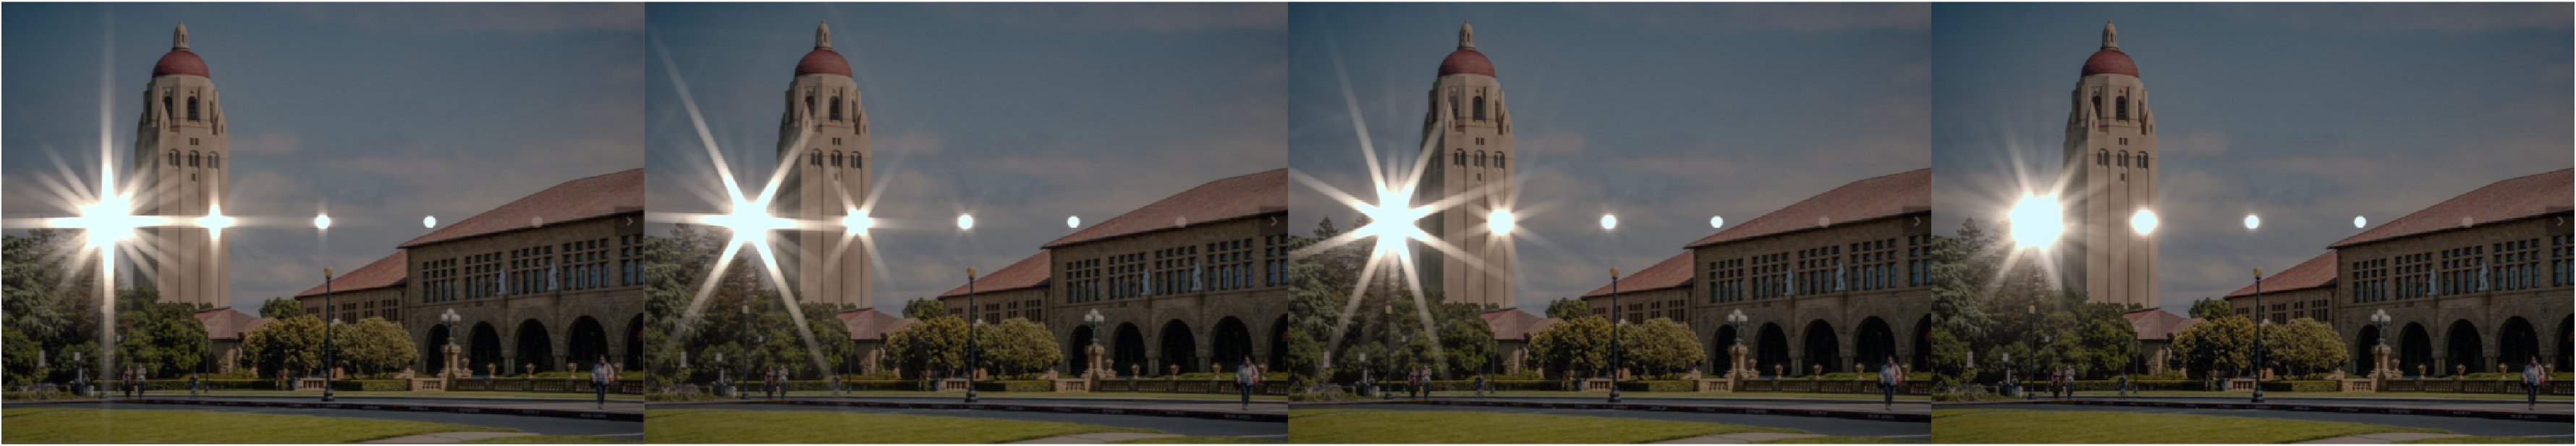
\includegraphics[width=0.9\textwidth,height=\textheight]{chapters/images/optics/06-geometric/pinhole-shape-hdr.png}

}

\caption{\label{fig-pinhole-hdr}High dynamic range images simulated
through a lens with a regular polygon aperture.}

\end{figure}%

For the simulation in Figure~\ref{fig-pinhole-hdr}, I also added some
scratches and dust on to the lens for realism. The brightest light in
each scene (left) is five orders of magnitude (\(10^5\)) more intense
than the dimmest light (right), which is barely visible. The lights are
all the same size, but the bright ones appear larger because of the
blurring by the PSF.

\subsection{Human PSF}\label{human-psf}

Human eyes have approximately circular pupils. In bright light the pupil
is contracted to about 3 mm diameter, and the PSF can be roughly
circularly symmetric. In darker environments, the pupil widens and
imperfections of the human optics (cornea, lens) often have a very large
and irregular impact on the PSF. The pupil aperture is circular, but the
optical imperfections distort the PSF and it takes on a very irregular
shape (Thibos (2020) Thibos et al. (2002)).

Even though the PSF is quite irregular, we often approximate its shape.
One approximation summarizes whether or not the PSF is very different in
two directions. If it is very different in two perpendicular directions,
we say the person is \textbf{astigmatic}. Figure~\ref{fig-astigmatism}
shows PSFs with some defocus and astigmatism. These were simulated using
the same wavefront methods I described above and that will be covered in
Chapter~\ref{sec-optics-wavefront}.

\begin{figure}

\centering{

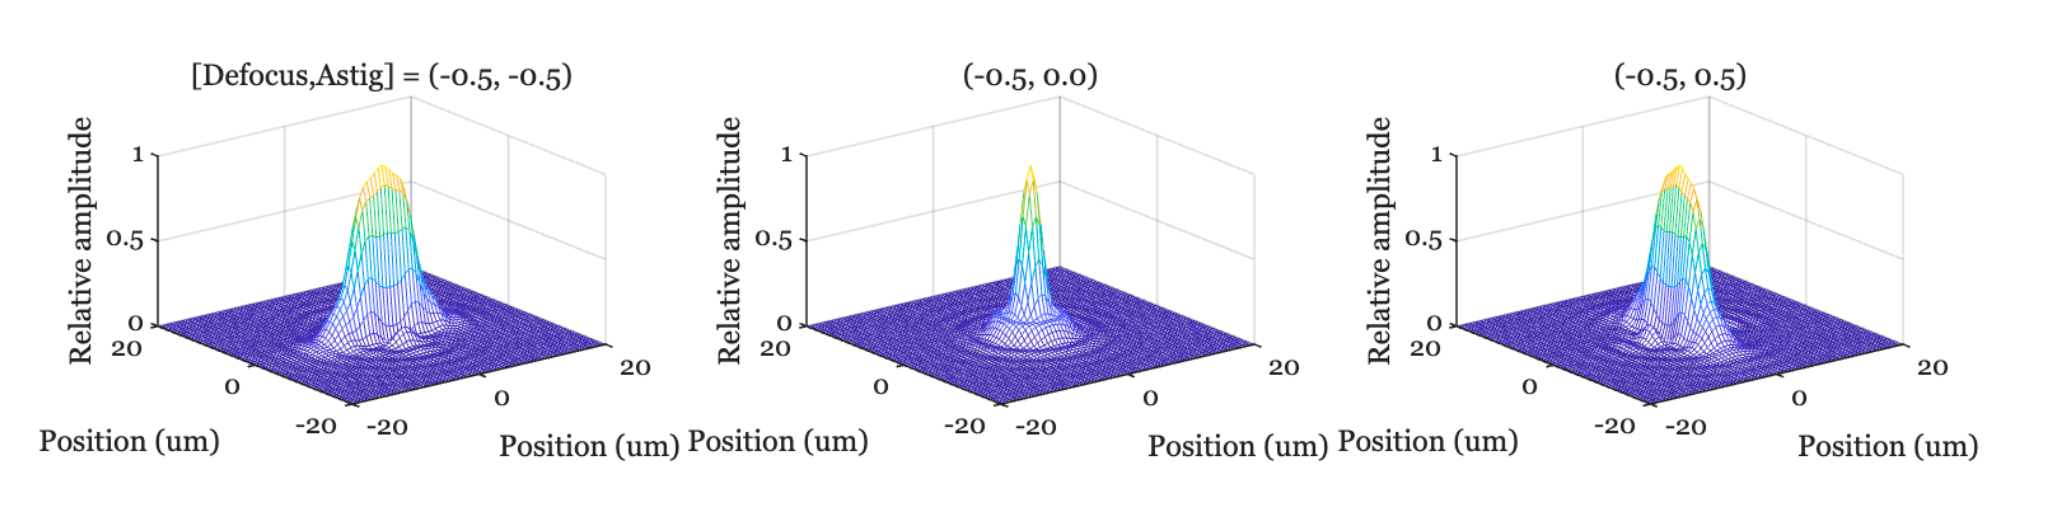
\includegraphics[width=1\textwidth,height=\textheight]{chapters/images/optics/06-geometric/astigmatism-defocus.png}

}

\caption{\label{fig-astigmatism}Illustration of astigmatism.
s\_wvfAstigmatism. Top row of the plot.}

\end{figure}%

I will show simulations of a range of human PSFs in
Chapter~\ref{sec-human}. You can assess your own PSF easily. Glasses or
contact lenses are typically designed to sharpen the PSF and counter any
astigmatism. To see the PSF of your lens, take off your glasses or
contact lenses, and look with one eye at a small spot of light in the
dark -maybe a night light from across the room, or one of the LED lights
on electronic gear- against in the presence of a uniform background such
as a wall. The image you see is the PSF of your own visual system. If
you are looking in a dark room, your pupil is probably relatively large.
By squinting, you reduce the size of your eye's aperture, and this is
likely to sharpen the PSF. The squinting reduces how much the lens
contributes to image formation. If the aperture is made quite small, say
by using an artifical pupile, the image will be diffraction limited.

\chapter{Lens principles}\label{sec-optics-lenses}

\section{Lens principles overview}\label{sec-optics-lenses-overview}

A small pinhole renders a perfectly good image. Why do we need to add
any optics? The critical reason is that pinhole apertures, by
definition, only measure a small amount of electromagnetic radiation. We
often find ourselves in conditions where the amount of radiation passing
through the aperture is a limiting factor. We need more signal!

Let me tell you what I mean by \textbf{small}. Suppose we are in a dim
room illuminated with a broad wavelength spectrum (10 \(cd/m^2\)).
Consider a camera with a 1 mm pinhole, a sensor with 1 micron pixels, a
focal length of 4mm, and an exposure duration of 50 milliseconds. In
that case only about 35 photons arrive at each pixel. If we want to see
in color, we must further divide up the wavelength range and the
situation worsens. Because of the inescapable photon noise, which I
describe later, this signal only permits a reliable intensity
discrimination when two pixels differ by more than 20\% (i.e., one edge
is 20\% brighter than the other, see
\href{../code/fise_opticsCountingPhotons.html}{fise\_opticsCountingPhotons}).

A lens, or more generally optics, is a way to enlarge the entrance
aperture to acquire more photons, without paying a big penalty in
spatial blur or geometric distortions. This ability must have great
value because the solution has been used by many different animal
species.

\begin{tcolorbox}[enhanced jigsaw, bottomtitle=1mm, titlerule=0mm, arc=.35mm, colbacktitle=quarto-callout-note-color!10!white, coltitle=black, toprule=.15mm, bottomrule=.15mm, breakable, colframe=quarto-callout-note-color-frame, left=2mm, opacityback=0, colback=white, title=\textcolor{quarto-callout-note-color}{\faInfo}\hspace{0.5em}{Optics in animals}, opacitybacktitle=0.6, toptitle=1mm, rightrule=.15mm, leftrule=.75mm]

The most primitive animal eyes are called `pigment cup'. These are made
of a small receptor surface, about 0.1mm in diameter, and the eye is
simply open. The size of the opening is a bit large to be considered a
pinhole. The eyes of some animals, in particular molluscs, have pinhole
architectures. The receptor surface itself is 10 mm in diameter, and the
opening is 0.4 - 2.8mm. These eyes evolved about 500 million years ago
and have little changed.

\begin{figure}[H]

\centering{

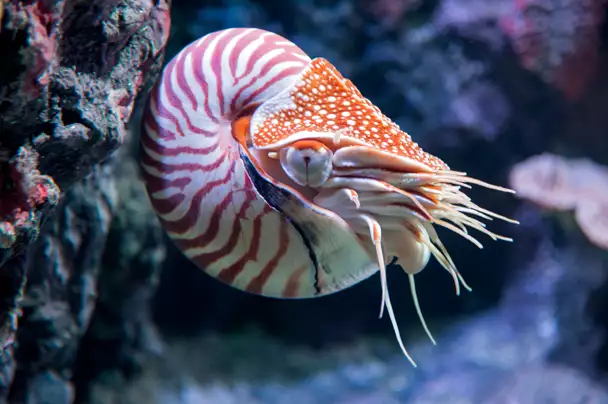
\includegraphics[width=0.7\textwidth,height=\textheight]{chapters/images/optics/07-principles/mollusc-pinhole-monterrybay.png}

}

\caption{\label{fig-mollusc}}

\end{figure}%

The vast majority of animals have evolved visual systems with a lens.
You might enjoy
\href{https://www.britannica.com/science/photoreception/Single-chambered-eyes}{this
lovely article by Michael Land}, a distinguished vision scientist who
taught us much about animal vision systems.

\end{tcolorbox}

\section{Rays and wavefronts}\label{rays-and-wavefronts}

In the section on thin lenses, we describe lenses and treat light as
rays (geometric optics). The reader may find this odd, given the clear
demonstration of light as waves \textbf{?@sec-lightfields-diffraction},
and the obvious failure of the ray model. But to model refraction, and
many other optics characteristics, geometric optics is both intuitive
and accurate. We will return to calculations using waves later, when we
consider more advanced calculations
(Chapter~\ref{sec-optics-wavefront}).

It is useful to draw the connection between geometric and wave
representations. In \textbf{wave optics} a collection of rays headed in
the same direction, and of the same wavelength and phase, are
represented as a plane wave (Figure~\ref{fig-waves-rays}). We can
visualize the wave by drawing a line through the peaks of their
(in-phase, common amplitude) waves. We call this line the
\textbf{wavefront}. The wavefront diagrams do not show the amplitude of
the wave. Various ray-wavefront combinations are illustrated in the
different panels of Figure~\ref{fig-waves-rays}.

\begin{figure}

\centering{

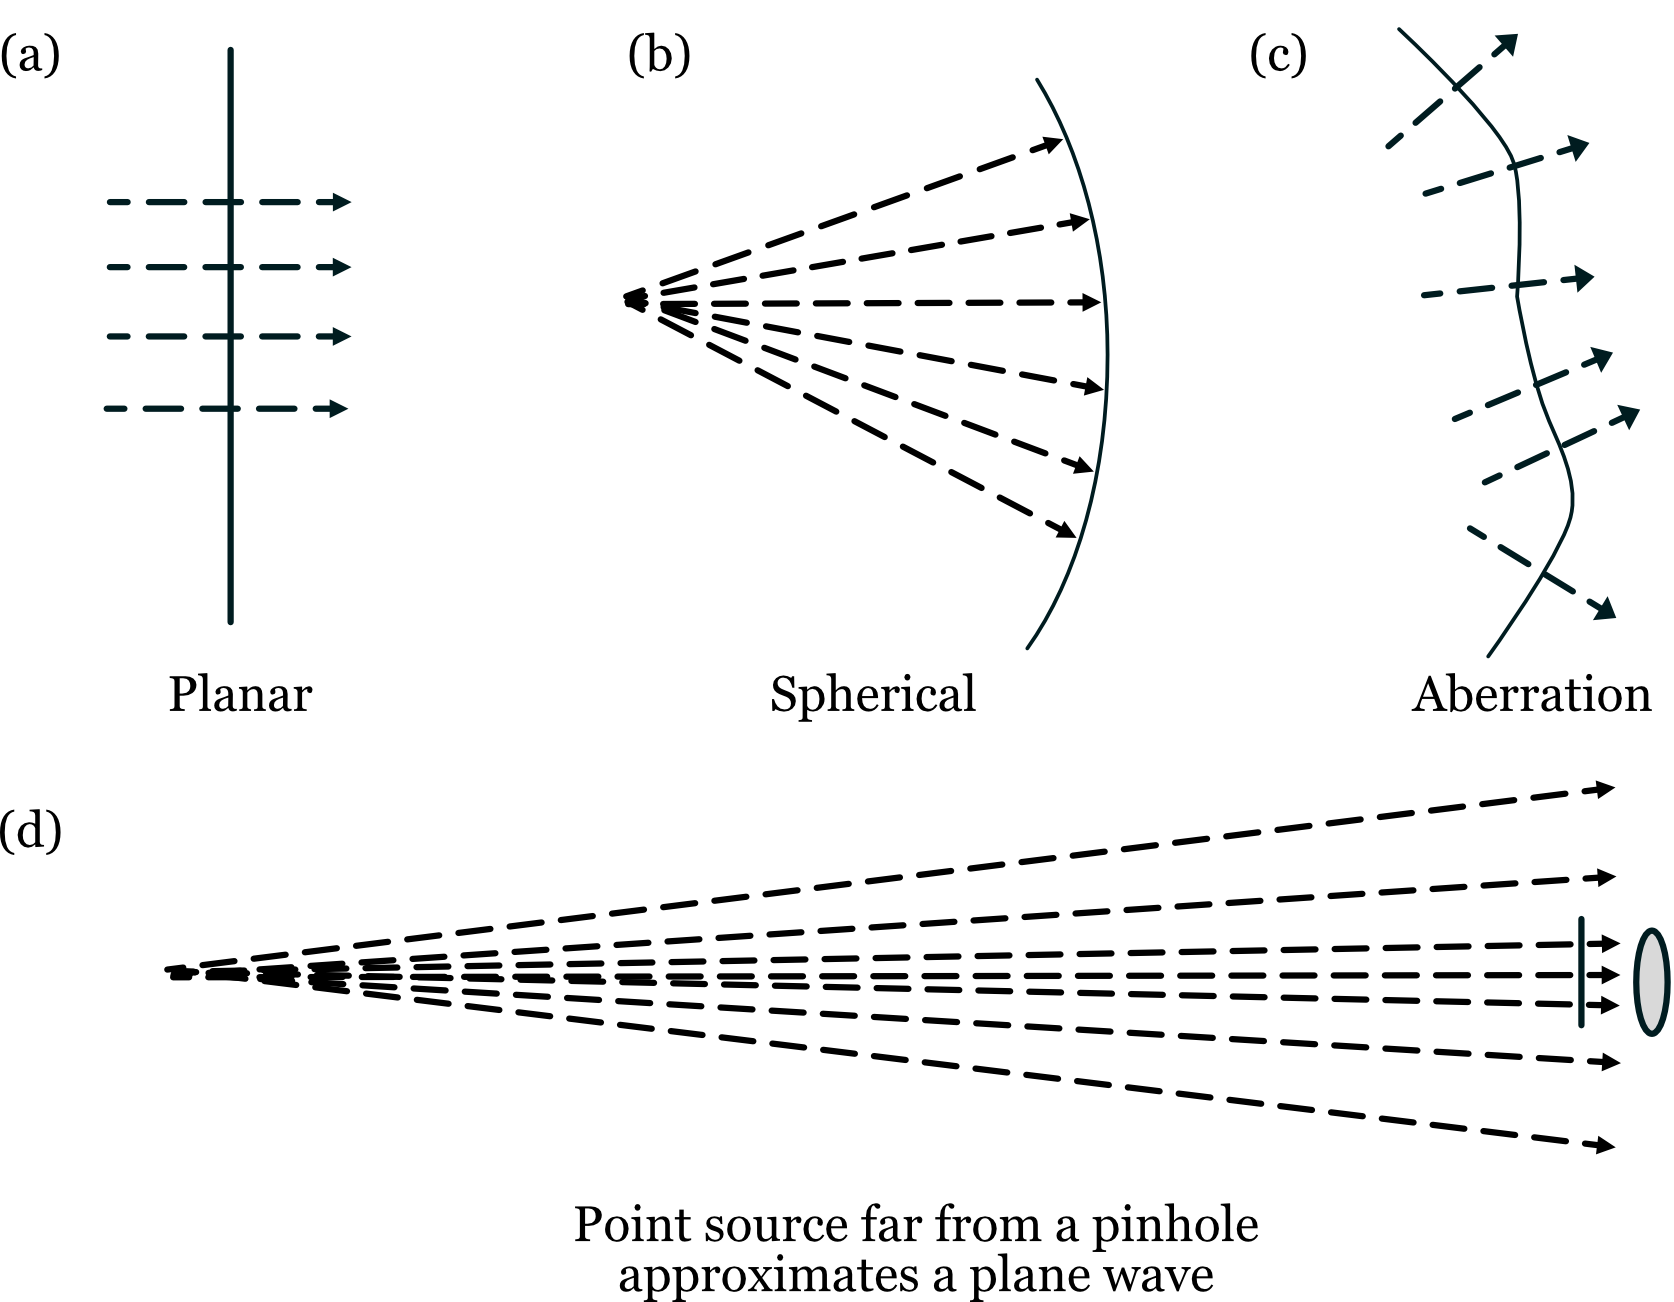
\includegraphics[width=0.75\textwidth,height=\textheight]{chapters/images/optics/07-principles/rays-wave.png}

}

\caption{\label{fig-waves-rays}Relationship between the ray (arrows) and
wavefront (dashed) representations. (a) A collimated set of rays is a
planar wavefront. (b) Rays from a point source form a spherical
wavefront. (The image shows a slice through the sphere). (c) Smoothly
varying wavefronts with many different shapes are common. Often these
shapes are due to imperfections (aberrations) in the optics. We reason
about them as a collection of rays; the direction of each ray is drawn
perpendicular to the tangent of the wavefront. (d) Only a narrow section
of the rays from a distant point are incident at the entrance aperture
of the imaging device. Hence, the incident light field from the point is
close to a planar wavefront.}

\end{figure}%

It is common for optics tutorials to represent wavefront directions as
extended in space, but it is uncommon to represent the amplitude of the
wavefront across space. In reality the amplitude of the wavefront will
vary across space. For example, a typical laser emits a set of parallel
(collimated) rays. The amplitude of these rays has a Gaussian profile
that limits the wavefront in space. That's why the spot a laser pointer
produces is limited in space. In recent years, image systems engineers
have had access to \textbf{spatial light modulators (SLMs)}. These
devices modulate either the local amplitude or phase of the wavefront at
different positions in space, controlling the light field.

The software calculations that accompany this book use both wavefront
and ray methods\footnote{The ISETCam optics calculations uses the wave
  model. The ISET3d graphics calculations use the ray model.}.

\section{Material interactions}\label{material-interactions}

When a light rays arrive at the boundary between regions with different
optical properties - whether those regions contain matter (like glass or
water), air or vacuum - several things can happen
(Figure~\ref{fig-reflected-scattered}). The rays might be reflected
back, as in a mirror. Or, the rays might enter into the material,
undergo a series of internal reflections, and emerge back in one of many
different directions. Also, the rays might enter the material and be
absorbed, giving up their energy to the atoms in the material. (Maybe
reference the dichromatic reflection model here?)

\begin{figure}

\centering{

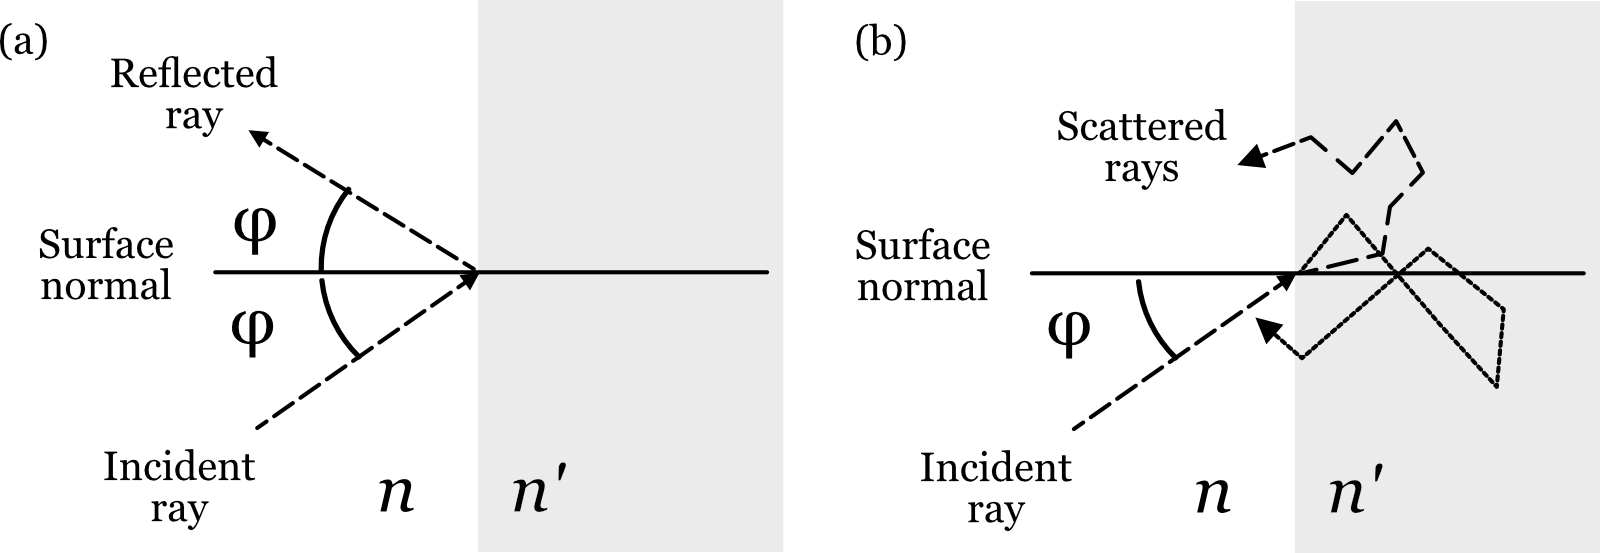
\includegraphics[width=1\textwidth,height=\textheight]{chapters/images/optics/07-principles/snell-reflected-scattered.png}

}

\caption{\label{fig-reflected-scattered}When rays arrive at the boundary
of two regions, The rays (a) might be reflected, (b) might enter the
medium, be internally reflected multiple times, and emerge in one of
many different directions (scattering). (Not shown) The ray may might
enter the medium and be absorbed.}

\end{figure}%

The most important case for controlling the rays, and thus for optical
design, is this other possibility: the ray enters the new material and
continues on its way. We call this change in direction
\textbf{refraction}.

\begin{figure}

\centering{

\includegraphics[width=0.5\textwidth,height=\textheight]{chapters/images/optics/07-principles/snell-refraction.png}

}

\caption{\label{fig-snell-law}A ray crossing the boundary between two
materials may continue but change direction. The change occurs because
the speed of electromagnetic waves differs between the regions. The
\emph{refraction index} (\(n\) and \(n'\)) is the material parameter
that describes the speed.}

\end{figure}%

\subsection{Snell's Law}\label{sec-snells-law}

Snell's Law quantifies how light changes direction when passing between
regions with different optical properties. The mathematical formulation
of Snell's Law is defined using the variables shown in
Figure~\ref{fig-snell-law}. A light ray (Incident ray) is shown crossing
a planar boundary between one medium (say, air) in a second medium (say,
glass). The angle between the incident ray and a line perpendicular to
the surface (the surface normal) is \(\phi\). The refracted ray changes
direction and thus has a different angle, \(\phi '\), with respect to
the surface normal. Snell's Law captures the relationship between these
two ray angles

\begin{equation}\phantomsection\label{eq-snell}{ 
n \sin(\phi) = n' \sin(\phi') 
}\end{equation}

The variables \(n\) and \(n'\) are the \emph{refraction index} of the
materials, which is related to the speed of the electromagnetic
radiation in the material.

\begin{equation}\phantomsection\label{eq-indexofrefraction}{ 
n = \frac{c}{v} 
}\end{equation}

where \(c\) is the speed of light in a vacuum, \(v\) is the speed in the
material. By definition, \(n=1\) in a vacuum. It is very close to
\(1.0\) in air. In some materials, such as glass, the velocity of light
is much slower, so that the index might be \(1.3\) or even \(1.5\).

In many common materials the velocity is reduced because the light,
which is electromagnetic radiation, induces an electrical signal in the
electrons of the material. The specific properties of this signal depend
on the material. The induced electrical signal sums with the electrical
field of the light. The combined signal is predicted to travel slower
and in a different direction, with the exact change in speed and
direction dependent on the electrical properties of the
material\footnote{This excellent pair of (nicely snarky) Fermilab videos
  from Don Lincoln explain the change in
  \href{https://www.youtube.com/watch?v=CUjt36SD3h8}{velocity} and
  \href{https://www.youtube.com/watch?v=NLmpNM0sgYk}{direction.}. We can
  thank James Clerk Maxwell for providing the basis of this
  understanding.}.

Interestingly, there are less common materials (e.g.,liquid crystals)
that have more complex interactions with the electrical field of light.
These materials create interesting and useful effects (birefringence)
that we will describe in Chapter~\ref{sec-displays}.

\begin{tcolorbox}[enhanced jigsaw, bottomtitle=1mm, titlerule=0mm, arc=.35mm, colbacktitle=quarto-callout-note-color!10!white, coltitle=black, toprule=.15mm, bottomrule=.15mm, breakable, colframe=quarto-callout-note-color-frame, left=2mm, opacityback=0, colback=white, title=\textcolor{quarto-callout-note-color}{\faInfo}\hspace{0.5em}{Why lenses bend light}, opacitybacktitle=0.6, toptitle=1mm, rightrule=.15mm, leftrule=.75mm]

This is a very nice tutorial from Fermilab about the physical basis of
refraction. The video takes on various (wrong) explanations first, and
then explains refraction using principles derived from Maxwell's
equations. Very clear and cool stuff.

\href{https://www.youtube.com/watch?v=NLmpNM0sgYk}{In this YouTube
tutorial, Don Lincoln of Fermilab explains why light bends when entering
glass.}

\end{tcolorbox}

\subsection{Wavelength dependence}\label{sec-chromatic-aberration}

For many materials that index of refraction is wavelength dependent.
Following Snell's Law, the each wavelengths changes direction by
different amount. Consequently, when we set the lens to be in best focus
for one wavelength, it will not be in best focus for other wavelengths.
The inability to produce a good focus for all wavelengths simultaenously
is called \textbf{chromatic aberration}.

For most materials the change of the refraction index over the visible
wavelength is roughly linear, just varying in extent. It is common to
summarize the dispersion using the \emph{Abbe number}, \(V_d\), which is
computed by comparing the refraction index at three different
wavelengths.

\begin{equation}\phantomsection\label{eq-abbe}{ 
V_d = \frac{n_{489.3} - 1}{n_{486.1} - n_{653.3}}
}\end{equation}

Conventionally, an Abbe number greater than 50 implies very little
dispersion and a number less than 30 implies significant dispersion that
will impact image quality. The human eye has very significant chromatic
aberration, with an Abbe number of about 15.

When possible, it is my preference in computation to provide numerical
values describing the index of refraction as function of wavelength and
to measure the impact by computing the line spread or point spread
function. We will perform analyses of chromatic aberration several times
in this book, including in Chapter~\ref{sec-human}.

\begin{tcolorbox}[enhanced jigsaw, bottomtitle=1mm, titlerule=0mm, arc=.35mm, colbacktitle=quarto-callout-note-color!10!white, coltitle=black, toprule=.15mm, bottomrule=.15mm, breakable, colframe=quarto-callout-note-color-frame, left=2mm, opacityback=0, colback=white, title=\textcolor{quarto-callout-note-color}{\faInfo}\hspace{0.5em}{Historical note: Refraction}, opacitybacktitle=0.6, toptitle=1mm, rightrule=.15mm, leftrule=.75mm]

Refraction was studied by the Greek astronomer Ptolemy in about the year
150. He documented that rays passing from air into, say water or glass,
change direction. Ibn Sahl in Persia, around 930, quantified the change
in direction as light crossed the boundary between certain materials,
and he used this knowledge to design lenses.

The formula for refraction was discovered independently by two
scientists in the 17th century. Willebrord Snellius (also known as
Snell) first found the mathematical relationship in 1621, but his work
wasn't published during his lifetime. He was an astronomer, and in 1617
he determined the size of the earth based on measurements of its
curvature between the cities of Alkmaar and Bergen-op-Zoom.

Renée Descartes independently discovered the relationship as well, and
he published it in 1637. Although Descartes published first, the formula
became known as Snell's Law to acknowledge Snell's earlier discovery. In
modern times, the French still frequently refer to Snell's Law as ``la
loi de Descartes'' or ``la loi de Snell-Descartes''.

The physicist Christiaan Huygens showed that Snell's Law could be
explained by treating light as a wave that travels at different speeds
in different materials. More about the history of the discovery and
quantification, including the references,
\href{https://en.wikipedia.org/wiki/Snell\%27s_law\#History}{makes for
interesting reading}.

\end{tcolorbox}

\section{Lenses control ray
directions}\label{lenses-control-ray-directions}

\begin{figure}

\centering{

\includegraphics[width=0.75\textwidth,height=\textheight]{chapters/images/optics/07-principles/pinhole-rays-lens.png}

}

\caption{\label{fig-pinhole-rays}(A) The rays from a nearby point that
pass through a relatively large pinhole diverge. They form an image of
the point that is larger than the pinhole. (B) Lenses transform the
direction of the rays in the incident light field, redirecting the rays
to converge at the image surface.Diffraction imposes a limit on the
precision of the convergence.}

\end{figure}%

Consider the rays from a point as they pass through a pinhole. The image
they form will not be sharp because the ray directions are diverging.
Narrowing the pinhole sharpend the image formation by selecting a small
subset of the rays.

We can sharpen the image by redirecting some the rays to converge at the
image plane. One way to think about optical devices is that they are
built to control the direction of the environmental light field rays at
the image system entrance aperture. When forming a sharp image is the
goal, we evaluate the optics by asking whether they adjust the ray
directions so that the image of a point in the scene is also a point. A
useful fact to remember is that diffraction means the best (sharpest) we
can do for a circular aperture is defined by the diameter of the Airy
disk.

\section{Making a lens}\label{making-a-lens}

To make a lens that focuses a light field into an image plane requires
changing the direction of many rays. The simple case of rays from one
point is easy to see.

\begin{figure}

\centering{

\includegraphics[width=0.5\textwidth,height=\textheight]{chapters/images/optics/07-principles/thinlens-prism.png}

}

\caption{\label{fig-thinlens-prism}Refraction transforms the rays
diverging from an object point (left) to converging to an image point
(right).}

\end{figure}%

Imagine that the rays are diverging from an object point at the left.
Were the rays passing through a pinhole, they would continue to diverge.
Refraction by the prism changes the direction of the rays at the from
upward to downward (upper prism). Similarly, refraction changes the ray
directions from downward to upward (lower prism). These two prisms
converge the rays from the object point onto a point on a properly
positioned image plane.

\begin{figure}

\centering{

\includegraphics[width=0.8\textwidth,height=\textheight]{chapters/images/optics/07-principles/thinlens-assembled.png}

}

\caption{\label{fig-thinlens-prism}A lens can be approximated as many
small prisms. The outline shows a spherical surface on the entrance and
exit side.}

\end{figure}%

Expanding on this idea, we can stack a collection of prisms to gather
more of the rays. Or, more likely, we might polish a glass surface to
have two spherical surfaces, forming a continuous form of the stacked
prisms. The entrance aperture of this lens can capture much more light
than a pinhole, and it guides the rays to converge. Spherical lenses are
quite popular because they are easy to manufacture. Using Snell's Law it
is relatively straightforward to calculate the refraction for a ray
arriving at any location on the sphere \footnote{Put the formula for
  refraction of a ray at a spherical lens in here.}.

The diagram makes it clear that there are many lens design choices. For
example, we might change the shape of the lens surfaces. Also, we might
use different materials in the prisms. What considerations would guide
such choices?

\section{Innovations in Lens Design}\label{innovations-in-lens-design}

An overarching goal in optical design is to create a lens that is free
from imperfections, known as aberrations. The choices in lens design
involve trade-offs between performance, cost, size, and weight. The
following sections introduce a range of solutions, from classical to
cutting-edge, that address these challenges.

\subsection{Spherical Aberration}\label{spherical-aberration}

Spherical surfaces are relatively easy to manufacture and thus
cost-effective. However, they have a fundamental flaw first documented
by the 11th-century scientist Alhazen in his ``Book of Optics''
(\emph{Kitāb al-Manāẓir}). He observed that spherical lenses produce
blurry images because they refract light more strongly near their edges
than near their center. As a result, rays passing through the periphery
of the lens do not converge at the same focal point as rays passing
through the center. This imperfection is called \textbf{spherical
aberration}. The severity of this aberration depends on factors like the
lens aperture, curvature, and material.

\subsection{Multi-element lens}\label{multi-element-lens}

A classical solution to spherical and other aberrations is to combine
multiple spherical lenses into a single optical system. In these
\textbf{multi-element optics}, additional lenses are carefully arranged
to cancel out the aberrations of the primary lens. Famous designs like
the \emph{Double-Gauss} or \emph{Petzval} lens systems use this
principle to achieve high image quality. While effective, this approach
often results in large, heavy, and complex assemblies, as seen in
high-end camera lenses. I will describe these classic designs in
Section~\ref{sec-optics-famous-lenses}. As you will see, in the early
days determining how to combine even a few spherical components was an
intellectual challenge, and quite important.

Modern optics with multiple elements has achieved very remarkable
advances. And, in some important cases, the size and weight are not a
limit. The important company, ASML, working with
\href{https://www.zeiss.com/semiconductor-manufacturing-technology/smt-magazine/duv-lithography.html}{Zeiss},
has produced entirely remarkable lenses. These enable people to use
lithography to manufacture of integrated circuits at nanometer
resolution. Now that's a lens.

\begin{figure}

\centering{

\includegraphics[width=0.6\textwidth,height=\textheight]{chapters/images/optics/07-principles/zeiss-lithography.jpg}

}

\caption{\label{fig-zeiss-lithography}ASML-Zeiss lens}

\end{figure}%

\subsection{Aspheric Lenses}\label{aspheric-lenses}

Instead of adding more lenses, another approach is to change the shape
of the lens surface itself. An \textbf{aspheric lens} deviates from a
perfect spherical shape, with its curvature changing from the center to
the edge. This tailored profile allows it to correct for spherical
aberration in a single element, enabling more compact and lightweight
designs.

Historically, aspheric lenses were difficult and expensive to produce.
However, advances in computer-controlled polishing and glass/plastic
molding have made them common in everything from smartphone cameras to
research-grade instruments. The surface of an aspheric lens, its
\emph{sag} \(z\), is often described as a function of the radial
distance \(\rho\) from the optical axis:

\begin{equation}\phantomsection\label{eq-aspheric}{
z(\rho) = \frac{\rho^2 / R}{1 + \sqrt{1 - (1 + k)(\rho/R)^2}} + A_4 \rho^4 + A_6 \rho^6 + \cdots
}\end{equation}

Here, \(R\) is the radius of curvature at the lens vertex, \(k\) is the
conic constant that defines the basic shape (e.g., parabolic,
hyperbolic), and the \(A_i\) terms are higher-order coefficients that
fine-tune the surface to minimize aberrations.

\subsection{GRIN Lenses}\label{grin-lenses}

Another way to control light is to vary the material properties within
the lens instead of changing its surface shape. A \textbf{gradient-index
(GRIN)} lens has a refractive index that changes continuously within the
material, typically decreasing from the center to the edge.

Long before this became practical, in 1854, James Clerk Maxwell
theorized that such a gradient could eliminate spherical aberration in a
spherical lens, a design now known as the ``Maxwell fisheye.'' It was
later discovered that many animal eyes use this exact principle. While
more challenging to manufacture than aspheres, GRIN lenses offer unique
design possibilities, especially in compact systems like endoscopes.
Maxwell's work in this area -and later when we discuss his work in
color- are an example of the interplay between physics, engineering, and
biology.

\subsection{Spatial Light Modulators}\label{spatial-light-modulators}

What if a lens could be reconfigured on the fly? \textbf{Spatial light
modulators (SLMs)} are devices that can dynamically control the
properties of a light field on a pixel-by-pixel basis. They are
essentially programmable optical elements.

\begin{itemize}
\tightlist
\item
  \textbf{Phase SLMs}, often based on liquid crystal arrays, can locally
  alter the phase of light, effectively acting as a reconfigurable lens
  or diffraction grating. They can be used to correct for aberrations in
  real-time or to sculpt a light beam into a complex pattern.
\item
  \textbf{Amplitude SLMs}, which use technologies like MEMS
  (micro-electro-mechanical systems) mirrors, modulate the intensity of
  light at each pixel.
\end{itemize}

With pixel sizes on the order of microns and arrays containing millions
of elements, SLMs are powerful tools in adaptive optics, holography, and
advanced imaging systems. This figure shows a recent phase SLM with
extremely high resolution.

\begin{figure}

\centering{

\includegraphics[width=0.6\textwidth,height=\textheight]{chapters/images/optics/07-principles/slm-holoeye.png}

}

\caption{\label{fig-slm-holoeye}Holoeye phase spatial light modulator
based on reflective LCOS. Max resolution 4160 x 2464, pixel Pitch 3.74
µm, Active Area 15.56 x 9.22 mm (0.7″ Diagonal, 8 Bit, 60 Hz frame
rate). The small part is the SLM; the big part is the electronics.
\href{https://holoeye.com/products/spatial-light-modulators/gaea-2-phase-only/}{See
Holoeye}}

\end{figure}%

\subsection{Metalenses}\label{metalenses}

The most recent revolution in optics miniaturization comes from
\textbf{metalenses}. These are not lenses in the traditional sense but
are flat surfaces, like a sliver of glass, patterned with an array of
nanoscale structures (``meta-atoms''). Each nanostructure is smaller
than the wavelength of light and is engineered to impart a specific
phase shift to the light passing through it.

By arranging these meta-atoms in a precise pattern, a metalens can bend
light just like a conventional curved lens but without the bulk. This
technology promises to replace complex, multi-element systems with a
single, ultra-thin optical element. Researchers are developing
metalenses that can perform sophisticated tasks, such as focusing
different colors to the same point or routing specific wavelengths to
different locations (Catrysse et al. (2022), Catrysse and Fan (2023)).
While still an active area of research, metalenses have the potential to
fundamentally change optical design.

\section{Onward}\label{onward}

The next sections will take you through the logical development from the
simple thin lens to the analysis of a thick lens, and then to
multielement lenses. Those principles are the foundation that has led to
these developments.

\chapter{Thin lenses}\label{sec-optics-thinlens}

\section{Thin lenses overview}\label{sec-optics-thinlens-overview}

Many image system properties can be summarized by the geometric optics
of ray tracing. This analysis characterizes important performance
characteristics of an optical system, such as its focal length,
magnification, and depth of field. These optical properties can be
analyzed in a particularly simple and clear way if we consider very
simple thin lenses.

Starting with an analysis of a thin lens has much practical value.
First, many people, including both engineers and photographers, rely on
the thin lens ideas when they describe optical system characteristics.
Familiarity with these ray trace characterizations is important for
anyone working in the field of image systems engineering. Second, even
more complex image systems are often made from lenses that are well
approximated by a collection thin lenses. We will go on to see how to
extend the thin lens ideas to more complex systems in
Chapter~\ref{sec-optics-morelenses}.

This section explains ways to understand image system optics by ray
tracing. Important as it is, ray tracing is not up to the task of a full
image systems simulation. As we saw in
Chapter~\ref{sec-geometric-optics}, we will need to account for the wave
properties of light, for example to incorporate diffraction. We will
explain the methods used for simulating the spectral irradiance at the
sensor in subsequent chapters about linear systems
(Chapter~\ref{sec-optics-linear-space}) and wavefront calculations
(Chapter~\ref{sec-optics-wavefront}).

\section{What is a thin lens}\label{sec-optics-thinlensdefined}

If a lens width is much smaller than the \emph{radius of curvature} of
its two surfaces, it is called a \emph{thin lens}. The radius of the
circle that (at least approximately) conforms to the surface of the lens
is the radius of curvature. There is no universally agreed upon
numerical value for what is meant by much smaller, but it is common to
consider a lens whose width is one-tenth or less of the radius of
curvature to be a thin lens.

\begin{figure}

\centering{

\includegraphics[width=0.4\textwidth,height=\textheight]{chapters/images/optics/08-thinlens/thinlens-definition.png}

}

\caption{\label{fig-thinlens-definition}(a) This lens width is smaller
than the radius of the circle that matches its surface. The lens might
be considered thin. (b) This lens width is approximately equal to the
radius of curvature. It is not be a thin lens.}

\end{figure}%

\section{Focal points}\label{sec-optics-focalpoints}

Figure~\ref{fig-thinlens-focalpoints} shows the important concept of the
primary and secondary focal points of a convex and concave thin lens.
The primary focal point (F) is the location on the optical axis such
that any ray coming from it towards the lens travels parallel to the
axis after refraction. The distance from that point to the middle of the
lens is called the \emph{focal length}. The secondary focal point The
secondary focal point (F') is the axial point such that any incident ray
traveling parallel to the axis will, after refraction, proceed toward,
or appear to come from it. The secondary focal point has its own focal
length.

\begin{figure}

\centering{

\includegraphics[width=0.8\textwidth,height=\textheight]{chapters/images/optics/08-thinlens/thinlens-focalpoints.png}

}

\caption{\label{fig-thinlens-focalpoints}(a) The primary (F) and
secondary (F') focal points of a convex (left) and concave (right) thin
lens. Read the diagram with the light rays (dark, solid lines) traveling
from left to right. The dashed lines drawn on the concave lens are
virtual rays that are shown to clarify how the focal point is found. See
the text for an explanation.}

\end{figure}%

When examining the behavior of an equiconvex lens, two primary scenarios
emerge. In the first scenario, rays emanating from the primary focal
point (F) enter the lens and are refracted in such a way that they exit
traveling parallel to the main optical axis. Conversely, when parallel
rays enter the lens, they are refracted and converge towards the
secondary focal point (F'), demonstrating the lens's ability to redirect
light.

The equiconcave lens presents a contrasting optical behavior. When
incident rays enter the lens at various angles with the intention of
producing parallel rays, these rays converge at the primary focal point
(F) on the opposite side of the lens. Dashed lines can be used to trace
and illustrate this convergence. In a separate scenario, when parallel
rays enter the equiconcave lens, they diverge after refraction. If these
diverging rays are extended backward using dashed lines, they appear to
originate from the secondary focal point (F') on the opposite side of
the lens.

There are many useful calculations that one can explore with simple
lenses and ray tracing. Here, we cover the basics to give the reader
some of the terminology and a sense of how these systems are analyzed.
For a deeper dive, I suggest the reader look into some of the excellent
textbooks on optics (References here. Usually Goodman; Born and Wolf; I
like Jenkins and White.)

\section{Three ray tracing principles}\label{sec-optics-3principles}

Consider the vector object on the left of
Figure~\ref{fig-lensmaker-center}. A ray from the arrowhead that is
parallel to the axis will be refracted through the focal point. A ray
from origin of the vector, which is on the optical axis, will also pass
through the focal point. Finally, a ray from the arrowhead - and this is
new - that passes through the center of the lens will continue on a
straight path.

\begin{figure}

\centering{

\includegraphics[width=0.7\textwidth,height=\textheight]{chapters/images/optics/08-thinlens/lensmaker-center.png}

}

\caption{\label{fig-lensmaker-center}Tracing an object through the lens
to an image.}

\end{figure}%

In summary, rays that

\begin{itemize}
\tightlist
\item
  Enter parallel to the optical axis and pass through the focal point on
  the opposite side.
\item
  Pass through the center of the lens do not deviate (refract).
\item
  Pass through the primary focal point toward the lens exit parallel to
  the optical axis.
\end{itemize}

\section{Image plane}\label{sec-optics-imageplane}

They rays from a distant point off the optical approach the entrance as
parallel to one another but oblique to the optical axis. The ray that
passes through the center of the lens is called the \emph{chief ray}.
There will also be a ray that passes through the primary focal point. It
will be refracted by the lens and emerge as parallel to the optical
axis. These two rays intersect where the image of the point will be
formed.

\begin{figure}

\centering{

\includegraphics[width=0.6\textwidth,height=\textheight]{chapters/images/optics/08-thinlens/thinlens-obliquerays.png}

}

\caption{\label{fig-optics-focalplane}The image plane for distant points
is perpendicular to the optical axis and passes through the secondary
focal point (blue dashed line).}

\end{figure}%

\section{Lens power (diopters)}\label{sec-optics-lenspower}

The \emph{power} of a lens is the inverse of the focal length, in
meters. The unit for lens power, \(1/m\) is the \emph{diopter}. A short
focal length implies large power, either due to the curvature of the
lens surface or the refractive index of the lens material.

\begin{figure}

\centering{

\includegraphics[width=0.6\textwidth,height=\textheight]{chapters/images/optics/08-thinlens/lensparameters-power.png}

}

\caption{\label{fig-thinlens-power}Lens power is the inverse of focal
length. The unit of lens power is diopter.}

\end{figure}%

To measure the focal length of a lens we use a light source that
produces parallel rays at the entrance aperture of the lens. We then
slide the image plane back and forth, searching for the distance where
the spot is smallest. We can create parallel rays using many methods.
Perhaps the simplest is to use a small point source (e.g., an LED) at a
distance from the lens. The rays arriving at the lens will be a small
angular sliver of the emitted rays, and if the source is far from the
lens the rays will be very close to parallel (e.g.,
\textbf{?@fig-pinhole-basic}). An alternative, is to go outside on a
sunny day and use the sun as a source. The sun isn't small, but it is
really far away. By the time the rays from the disk of the sun arrive at
your lens, the rays will be parallel.

The optics in the human eye has multiple elements. Even so, we can
measure its focal length, which is about 0.016 m (\textasciitilde60
diopters). To bring objects at different distances into focus the optics
adjusts its power, a process called \emph{accommodation}. If it cannot
adjust adequately, we wear lenses (glasses, contact lenses) that
increase or decrease the optical power, say by 1-8 diopters, so that a
good image can be focused on the retina.

Young people can accommodate easily. As people age, we lose the ability
to change the optical power of the optics, a condition called
\emph{presbyopia}. This happens to everyone. This biological fact is a
consideration for the design of near field displays
(Chapter~\ref{sec-displays}).

\section{The lens formula}\label{sec-lens-formula}

When an object is far away, the rays arriving at the lens are parallel.
The image of the object will be in focus at the focal length. When the
object is closer, we can use the \emph{Lens formula} to find the plane
where the object will be in focus. This is called the \textbf{image
distance}. The equation, which was derived by Halley in 1693, relies on
the three ray tracing properties of symmetric thin lenses
(Section~\ref{sec-optics-3principles}). Using these principles, we can
locate where the object at a distance \(d_o\) will be in focused on the
image side; call that distance \(d_i\).

\begin{figure}

\centering{

\includegraphics[width=0.95\textwidth,height=\textheight]{chapters/images/optics/08-thinlens/lensmaker-similartriangles.png}

}

\caption{\label{fig-lens-formula-similartriangles}Similar triangles for
the lens formula.}

\end{figure}%

The rays in Figure~\ref{fig-lens-formula-similartriangles} identify two
pairs of similar triangles (cyan and yellow). On the left, we can see
that the triangles imply \(h_i/h_o = d_i/d_o\). On the right, we can see
that the triangle similarity implies \(h_i/h_o = \frac{d_i - f}{f}\).
Combining the two equalities, we have

\[\frac{d_i}{d_o} = \frac{d_i - f}{f} = \frac{d_i}{f} - 1 \]

rearranging terms, \[ 
\frac{d_i}{f}  = 1 + \frac{d_i}{d_o} 
\]

and dividing by \(d_i\) we have the lens formula

\begin{equation}\phantomsection\label{eq-lensformula}{ 
\frac{1}{f}    = \frac{1}{d_i} + \frac{1}{d_o} 
}\end{equation}

The common names for these variables are

\begin{itemize}
\tightlist
\item
  \(d_o\) - Object distance
\item
  \(d_i\) - Image distance
\item
  \(f\) - Lens focal length
\end{itemize}

\section{Image distance formula}\label{sec-optics-imagedistance}

Equation~\ref{eq-lensformula} defines a relationship between the object
distance and the image distance for a thin lens. We can rearrange the
terms.

\[
\frac{-1}{d_i} = \frac{1}{d_o} - \frac{1}{f}
\]

Notice that when \(d_o = \infty\), then \(d_i = f\). We can re-write the
formula to calculate the image distance explicitly.

\begin{equation}\phantomsection\label{eq-imagedistance}{
d_i = \frac{1}{\frac{1}{f} - \frac{1}{d_o}} = \frac{f~d_o}{d_o - f} 
}\end{equation}

You can see from Equation~\ref{eq-imagedistance} that as \(d_o\) becomes
much larger than \(f\), \(d_i\) becomes approximately \(f\).
Specifically, if we express \(d_o\) in terms of the focal length of the
lens, \(k f\), we have

\begin{equation}\phantomsection\label{eq-imagedistance}{
d_i = \frac{f k f}{(k-1) f} = f \frac{k}{k-1}
}\end{equation}

This script plots the image distance as a function of object distance
expressed as a multiple of focal length.

\section{Lensmaker equation}\label{sec-optics-lensmaker}

The lens formula (Equation~\ref{eq-imagedistance}) relates the image
distance, object distance, and focal length. The \textbf{lens maker
equation} explains how to calculate the focal length of a thin lens. The
formula applies to a thin lens with two spherical sides embedded in a
homogeneous environment. To apply the formula, we must know the radius
of curvature of the two sides of the lens as well as the index of
refraction of the lens material and its surrounding medium.

Here is the formula:

\begin{equation}\phantomsection\label{eq-lensmaker}{
\frac{1}{f} = (\frac{n_2}{n_1} - 1) ( \frac{1}{R_1} - \frac{1}{R_2}) 
}\end{equation}

Where - \(n_2\) is the refractive index of the lens - \(n_1\) is the
refractive index of the surrounding medium - \(R_1\), \(R_2\) are the
radii of curvature of the two surfaces

Here is a link to a very nice
\href{https://www.khanacademy.org/science/in-in-class-12th-physics-india/in-in-ray-optics-and-optical-instruments/in-in-refraction-in-thin-lenses/v/lens-makers-formula}{Khan
Academy video derivation of the formula}.

\section{Biconvex lenses}\label{sec-optics-biconvex}

The lenses drawn in Figure~\ref{fig-thinlens-focalpoints} are symmetric
(i.e., equiconvex and equiconcave), so it is not surprising, therefore,
that the focal lengths of the primary and secondary focal points are
equal. It is more surprising to learn that even if a thin lens has a
different curvature on the two sides, the two focal lengths will still
be equal Figure~\ref{fig-thinlens-asymmetric}. Such lenses are called
\textbf{biconvex}.

The symmetry follows from the formula in Equation~\ref{eq-lensmaker}.
Exchanging the two radii of curvature simply changes the sign of the
focal length.

\begin{figure}

\centering{

\includegraphics[width=0.5\textwidth,height=\textheight]{chapters/images/optics/08-thinlens/thinlens-asymmetric.png}

}

\caption{\label{fig-thinlens-asymmetric}Different radii of curvature for
a thin lens.}

\end{figure}%

\section{\texorpdfstring{The \(\mathrm{f}/\#\)
(f-number)}{The \textbackslash mathrm\{f\}/\textbackslash\# (f-number)}}\label{sec-optics-fnumber}

The \(~\mathrm{f}/\#\) of a thin lens is the ratio of its focal length
and entrance aperture diameter (Figure~\ref{fig-fnumber}). For example,
when we write f/4, it means that the focal length is 4x the aperture
diameter.

\begin{figure}

\centering{

\includegraphics[width=0.5\textwidth,height=\textheight]{chapters/images/optics/08-thinlens/lensparameters-fnumber.png}

}

\caption{\label{fig-fnumber}Graphic of the \(\mathrm{f}/\#\).}

\end{figure}%

The \(~\mathrm{f}/\#\) is an important parameter for all thin lenses;
this ratio appears in many formulae describing lens performance. It is
the key parameter that defines many properties of a circular,
diffraction-limited thin lens. Studying diffraction-limited lenses is an
important case for evaluating image system performance because it
represents an upper bound on the optical component; we cannot improve
the image system performance by using better optics.

As an example, remember the formula for the Airy disk diameter (meters)
on the image plane of a diffraction limited lens
(Equation~\ref{eq-airy1}) in \textbf{?@sec-lightfields-diffraction}.
That equation depends on the wavelength of light and the ratio of the
focal length and aperture, which is the \(\mathrm{f}/\#\). Re-writing
that formula, for a wavelength of \(\lambda\) and an \(~\mathrm{f}/\#\),
we have

\begin{equation}\phantomsection\label{eq-airy2}{ 
d = 2.44 ~ \lambda ~ N
}\end{equation}

\section{Magnification and zoom}\label{sec-optics-zoom}

Consider the simple thin lens in Figure~\ref{fig-optics-magnification}
with a image distance of \(f = 0.1m\). We draw the rays to the image
plane for an object at a distance of \(d_o = 0.3m\).

\begin{figure}

\centering{

\includegraphics[width=0.9\textwidth,height=\textheight]{chapters/images/optics/08-thinlens/lensparameters-magnification.png}

}

\caption{\label{fig-optics-magnification}Ray tracing lenses with
different focal lengths. Suppose focal length of the lens in the bluish
box is \(0.1 m\) and the distance to the object as \(0.3m\). And suppose
the focal length in the greenish box is \(0.2 m\).}

\end{figure}%

Using the lens formula, the image distance for the lens in the bluish
box is

\[
d_i = \frac{f \times d_o}{d_o - f} = \frac{0.1 \times 0.3}{0.3 - 0.1} = 0.15 m
\]

The image distance for the lens in the greenish box, with twice the
focal length, \(f' = 0.2m\), is

\[
d_{iL} = \frac{0.2 \times 0.3}{0.3 - 0.2} = 0.60 \text{m}
\]

The image distance and image size both increase by a factor of \(4\).
The two lenses have the same entrance aperture, so they capture the same
amount of light. Because the longer focal length lens spreads the image
over a larger area, the amount of light per unit area (irradiance) in
the image is reduced.

Some camera optics with an adjustable focal length, and this enables the
user to adjust the image magnification. The image sensor size, however,
is usually fixed. Thus, if we increase the image magnification, the
fixed sensor captures a smaller portion of the image, but with the same
sensor spatial resolution. The effect is to produce an image that
appears to zoom into a portion of the image. This technique, called
\textbf{optical zoom} is very effective as long as there is no loss of
spatial resolution in the magnified image.

\begin{figure}

\centering{

\includegraphics[width=0.8\textwidth,height=\textheight]{chapters/images/optics/08-thinlens/lensparameters-zoom.png}

}

\caption{\label{fig-optics-zoom}Optical zoom. (a) A small image that
just fits onto the sensor (dashed lines). (b) If we magnify the image,
say by increasing the focal length and image distance, the sensor
measures a smaller portion of the image. This is optical zoom.}

\end{figure}%

\section{\texorpdfstring{\(\mathrm{f}/\#\) and image
intensity}{\textbackslash mathrm\{f\}/\textbackslash\# and image intensity}}\label{sec-optics-fnumberintensity}

Suppose we wish to magnify the image, but we want to maintain the image
irradiance level. In that case, we must capture \(4\) times as much
light. We do this by increasing the lens diameter, \(D\). The formula
for the area of the aperture is \(\pi (D/2)^2\); thus, doubling the
diameter, \(D\), increases the area by a factor of \(4\).

The size of the lens with the larger diameter is sketched by the dashed
ellipse in the green section of Figure~\ref{fig-optics-magnification}.
Increasing the focal length expands the image size and reduces the image
intensity. Increasing the lens diameter compensates for the reduced
intensity. Doubling the focal length and entrance diameter preserves the
f/\# (ratio of the focal length and the aperture diameter). This example
illustrates that lenses with the same f/\# produce images with the same
image intensity.

\section{Depth of field}\label{sec-optics-dof}

Equation~\ref{eq-imagedistance} tells us how to set the distance between
the optics and image plane, \(d_i\), to bring an object at distance
\(d_o\) into focus. We might also be interested to answer the related
question: Given that an object at \(d_o\) is in focus, what will the
blur be for objects nearer or further? The range of distances over which
the objects remain in good focus is called the \textbf{depth of field}.

The size of the depth of field can be controlled by adjusting the size
of the lens aperture. As it becomes smaller, the lens becomes closer to
a pinhole, the depth of field increases. The depth of field can become
quite narrow for a large aperture. Controlling the depth of field can
create visually interesting images (Figure~\ref{fig-optics-bokeh}).
Photographers and cinematographers often use settings to bring the main
object of interest into good focus and blurring the rest. The depth of
field is a quantitative description of the lens setting. Photographers
use the term \textbf{bokeh} to describe the aesthetic impact one can
achieve by adjusting the depth of field. This quality depends on the
optics as well as the scene contents.

\begin{figure}

\centering{

\includegraphics[width=0.8\textwidth,height=\textheight]{chapters/images/optics/08-thinlens/optics-bokeh.png}

}

\caption{\label{fig-optics-bokeh}The depth of field is controlled by the
size of the lens aperture. (A) Photographers often adjust the depth of
field to bring the main object into focus, allowing other parts of the
scene to become defocused. (B) If we fix the image distance, increasing
the \(\mathrm{f}/\#\) decreases the aperture, making the lens
increasingly like a pinhole camera. For a large \(\mathrm{f}/\#\), the
depth of field becomes quite larger.}

\end{figure}%

\subsection{Circle of confusion}\label{sec-optics-coc}

Consider an image formed with a thin lens that is kept at a fixed
distance from the image plane (Figure~\ref{fig-optics-coc1}). The middle
image panel an object in excellent focus, and the other two panels show
points that are too near or too far. As the point moves away from the
in-focus object distsance, in either direction, the image will be a
roughly circular region increases in diameter. This is the circle of
confusion. This is the \textbf{circle of confusion}. It is a useful
concept that is specifically helpful for understanding and quantifying
the depth of field.

\begin{figure}

\centering{

\includegraphics[width=0.4\textwidth,height=\textheight]{chapters/images/optics/08-thinlens/optics-coc-1.png}

}

\caption{\label{fig-optics-coc1}Circle of confusion}

\end{figure}%

Notice that narrowing the aperture reduces the angle of the rays that
arrive at the sensor (Figure~\ref{fig-optics-coc2}). As the angle
narrows, the image size of an out-of-focus point shrinks. If the point
is already in focus, however, the rays are arriving at the same point
and the image size is little changed. This is the same idea we observed
in \textbf{?@sec-lightfields-diffraction} when we explained pinhole
cameras. This diagram makes clear that a pinhole camera has a very large
depth of field. No Bokeh for the pinhole afficianados!

\begin{figure}

\centering{

\includegraphics[width=0.4\textwidth,height=\textheight]{chapters/images/optics/08-thinlens/optics-coc-2.png}

}

\caption{\label{fig-optics-coc2}Narrowing the aperture changes the
angular range of the rays at the image plane. The original rays are
shown in gray and the rays that pass through the aperture are again
shown in blue. Because of the reduction in angle, the image blur is
reduced (shown at the right). Thus, the diameter of the circle of
confusion is reduced as well.}

\end{figure}%

We can use the diameter of the circle of confusion to quantify the depth
of field. The diameter depends on the parameters of the lens and image
plane (Figure~\ref{fig-optics-coc3}). The size of the circle of
confusion is computed by the ISETCam function
\href{https://github.com/iset/ISETCam/blob/main/opticalimage/optics/opticsCoC.m}{opticsCoC}.

\begin{figure}

\centering{

\includegraphics[width=0.6\textwidth,height=\textheight]{chapters/images/optics/08-thinlens/optics-coc-3.png}

}

\caption{\label{fig-optics-coc3}Narrowing the aperture reduces the size
of the circle of confusion. Notice that the vertical axis is
logarithmic, so that the change in diameter is substantial. Both lenses
have a 50 mm distance to the image plane. One lens has an
\(\mathrm{f}/\#\) of 2 (aperture=25 mm). The other lens has an
\(\mathrm{f}/\#\) of 8 (aperture=6.25 mm).}

\end{figure}%

Suppose we select a circle of confusion diameter that we consider to be
good focus. From the curves in Figure~\ref{fig-optics-coc3}, the depth
range of good focus will be relatively narrow for the large aperture
compared to the small aperture.

\begin{tcolorbox}[enhanced jigsaw, bottomtitle=1mm, titlerule=0mm, arc=.35mm, colbacktitle=quarto-callout-note-color!10!white, coltitle=black, toprule=.15mm, bottomrule=.15mm, breakable, colframe=quarto-callout-note-color-frame, left=2mm, opacityback=0, colback=white, title=\textcolor{quarto-callout-note-color}{\faInfo}\hspace{0.5em}{Deriving the CoC formula}, opacitybacktitle=0.6, toptitle=1mm, rightrule=.15mm, leftrule=.75mm]

The diameter of the circle confusion can be calculated using this
geometry. Suppose the image plane is placed so that a point \(P\) is in
focus, so that the distance to the image plane is \(f_P\). Another
point, \(X\), is closer and thus its focus would be beyond the image
plane, say at \(f_X\).

\begin{figure}[H]

\centering{

\includegraphics[width=0.4\textwidth,height=\textheight]{chapters/images/optics/08-thinlens/optics-coc-callout.png}

}

\caption{\label{fig-optics-coc-callout}Geometric demonstration of the
circle of confusion size.}

\end{figure}%

There will be two similar right triangles. One is formed with the sides
\(A/2\) (half the aperture) and \(f_X\); the similar triangle (blue) has
sides \(f_X - f_P\) and \(C_r\) (the radius of the circle of confusion).
Because the right triangles are similar, the sides must satisfy \[
\frac{C_r}{A/2} = \frac{f_X - f_P}{f_X}
\]

The diameter of the circle of confusion is twice the radius,
\(C = 2*C_r = A \frac{f_X - f_P}{f_X}\)

\end{tcolorbox}

\subsection{Depth of field formula}\label{sec-optics-dof-formula}

The depth of field formula quantifies the range of object distances that
appear acceptably sharp in an image. It is widely used as an
approximation, as we approximate an optical system as a thin lens:

\begin{equation}\phantomsection\label{eq-optics-depthoffield}{
\text{DOF} \approx 2 N C ({\frac{d_o}{f}})^2
}\end{equation}

where:

\begin{itemize}
\tightlist
\item
  \(N\) is the lens \(\mathrm{f}/\#\) (focal ratio, dimensionless)
\item
  \(C\) is the acceptable diameter of the circle of confusion (in
  meters)
\item
  \(d_o\) is the object distance (in meters)
\item
  \(f\) is the lens focal length (in meters)
\end{itemize}

Recall that \(N = f/A\), where \(A\) is the aperture diameter.
Substituting this into the formula gives:

\[
\frac{N}{f^2} = \frac{f}{A} \cdot \frac{1}{f^2} = \frac{1}{A f}
\]

So, the DOF formula can also be written as:

\[
\text{DOF} \approx \frac{2 C (d_o)^2}{A f}
\]

This relationship shows:

\begin{itemize}
\tightlist
\item
  DOF increases with object distance (\(d_o\))
\item
  DOF increases with the allowable circle of confusion (\(C\))
\item
  DOF decreases as aperture diameter (\(A\)) increases (i.e., with a
  larger aperture)
\item
  DOF decreases as focal length (\(f\)) increases
\end{itemize}

\textbf{Example:}\\
The plot below shows the DOF for a 100 mm focal length,
diffraction-limited lens, as a function of \(\mathrm{f}/\#\) and object
distance. The calculations use the ISETCam script
\href{https://github.com/iset/ISETCam/blob/main/scripts/optics/focus_dof/s_opticsDoF.m}{s\_opticsDoF},
which calls
\href{https://github.com/iset/ISETCam/blob/main/opticalimage/optics/opticsDoF.m}{opticsDoF}
to implement Equation~\ref{eq-optics-depthoffield}.

\begin{figure}

\centering{

\includegraphics[width=0.6\textwidth,height=\textheight]{chapters/images/optics/08-thinlens/optics-dof-image.png}

}

\caption{\label{fig-optics-dof}Depth of field in meters (z-axis) at
different object distances and thin lens approximation \(\mathrm{f}/\#\)
values.}

\end{figure}%

\chapter{Lenses and ray transfer}\label{sec-optics-morelenses}

\section{Lenses and ray transfer
overview}\label{sec-optics-morelenses-overview}

The principles of geometric optics and thin lenses are also critical for
thick lenses and multi-element
lenses(Chapter~\ref{sec-geometric-optics}). The first lens is traced,
and its output is the input to a second lens. We can use the three
principles (Section~\ref{sec-optics-3principles}) to analyze the lenses
in sequence. Using these tools, but with increasing complexity, the
methods used to characterize thin lenses
(Chapter~\ref{sec-optics-thinlens}) can be extended to many different
optical functions.

In this chapter, I will illustrate some of the extensions to thick
lenses and multi-element lenses. These have been important historically,
and they will continue to be with us for some years.

But a main goal is to lead you to the next level of optics, and in
particular the notion of the \emph{ray transfer matrix} and the
\emph{ray transfer function (RTF)} first introduced in
\textbf{?@sec-optics-metalens}. This idea conceptualizes optics in terms
of how the rays in the incident light field are transformed into the
rays in the optical light field. Characterizing a system in terms of a
transformation, in this case a function that transforms the rays from
one ight field into another, is an abstraction that is applicable to
many aspects of image systems engineering. Conceiving of the pipeline as
a series of transformaqtions, from capture to display, organizes how we
think of simulations. The approach may even apply to image
understanding.

But let's start here, with increasingly complex optics.

\section{Combining two thin lenses}\label{combining-two-thin-lenses}

Let's take a simple step towards more complex optical systems by
combining two thin lenses. When we place two lenses in series, the image
formed by the first lens becomes the object for the second.

If the lenses have focal lengths \(f_1\) and \(f_2\) and are separated
by a distance \(d\), the \emph{effective focal length} (\(f\)) of the
combination is given by:

\begin{equation}\phantomsection\label{eq-two-thin-lens}{
\frac{1}{f} = \frac{1}{f_1} + \frac{1}{f_2} - \frac{d}{f_1 f_2}
}\end{equation}

This formula gives the focal length of an \emph{equivalent} single thin
lens. However, it's important to remember that this equivalent lens
isn't located at the position of either of the original lenses. Its
position is defined by the system's principal planes, which we'll
discuss more in the context of thick lenses.

Recalling that the power of a lens (in diopters) is the inverse of its
focal length, Equation~\ref{eq-two-thin-lens} shows that: * When the
lenses are touching (\(d \approx 0\)), their powers simply add up:
\(P = P_1 + P_2\). * As the lenses are separated, the total power
changes. If \(d = f_1 + f_2\), the total power becomes zero
(\(f = \infty\)). This specific arrangement is called a \emph{focal
telescope}, and it collimates light, meaning parallel incoming rays
emerge as parallel outgoing rays.

A more practical value is the \textbf{back focal length (BFL)}, which is
the distance from the back surface of the last lens to the system's
final focal point. For our two-lens system, this is:

\begin{equation}\phantomsection\label{eq-back-focal-length}{
\text{BFL} = \frac{f_2 (d - f_1 )}{d - (f_1 + f_2)}
}\end{equation}

The BFL tells you exactly where to place a sensor to capture a sharp
image of an object at infinity. Notice that when \(d = f_1 + f_2\), the
denominator is zero, and the BFL becomes infinite, which is consistent
with the parallel rays produced by a focal telescope.

\href{https://phys.libretexts.org/Bookshelves/University_Physics/Physics_(Boundless)/24\%3A_Geometric_Optics/24.3\%3A_Lenses\#:~:text=The\%20focal\%20length\%20of\%20a,surfaces\%20are\%20convex\%20or\%20concave.}{See
around equations 24.3.4}

\section{Thick lens definitions}\label{thick-lens-definitions}

The principles of refraction and ray tracing apply to both thin and
thick lenses. However, for a \textbf{thick lens}, the optical design
calculations must account for the distance rays travel \emph{within} the
lens material. This internal propagation distance is assumed to be zero
in thin lens calculations, which is a key simplification.

We can extend the three principles used for thin spherical lenses
(Section~\ref{sec-optics-3principles}) to analyze thick lenses. The
concept of the focal point remains the same: Rays arriving parallel to
the optical axis converge toward the image-side focal point (\(F_2\)).
Conversely, rays passing through the object-side focal point (\(F_1\))
emerge parallel to the optical axis.

\begin{figure}

\centering{

\includegraphics[width=0.6\textwidth,height=\textheight]{chapters/images/optics/09-morelens/cardinal-points.png}

}

\caption{\label{fig-cardinal-points}Nodal points and principal planes of
a thick lens.}

\end{figure}%

For a thin lens, we noted that a ray passing through the optical center
is undeviated. A thick lens has a similar concept, but it involves two
\textbf{nodal points} (\(N_1\) and \(N_2\)). A ray directed toward the
object-side nodal point (\(N_1\)) emerges from the lens as if it came
from the image-side nodal point (\(N_2\)), traveling parallel to its
original direction (Panel A, Figure~\ref{fig-cardinal-points}).

To handle the ray's path, it is also convenient to define two
\textbf{principal planes} (\(P_1\) and \(P_2\)). Consider rays parallel
to the optical axis entering the lens. They exit the lens converging
toward the focal point. If we extend the incoming parallel ray forward
and the outgoing converging ray backward, they intersect. The locus of
these intersection points for rays near the optical axis forms the
image-side principal plane, \(P_2\) (Panel B,
Figure~\ref{fig-cardinal-points}). A similar construction using rays
from the front focal point defines the object-side principal plane,
\(P_1\). The intersection of a principal plane with the optical axis is
called a \textbf{principal point}.

In the general case, a thick lens is characterized by six
\textbf{cardinal points}: two focal points, two principal points, and
two nodal points. However, in the common situation where the medium on
both sides of the lens is the same (e.g., air), the nodal points
coincide with the principal points. This simplifies the system
considerably (Figure~\ref{fig-thick-cardinal}).

\begin{figure}

\centering{

\includegraphics[width=0.9\textwidth,height=\textheight]{chapters/images/optics/09-morelens/thick-cardinal-defintions.png}

}

\caption{\label{fig-thick-cardinal}Thick spherical lens definitions. By
convention, light travels from left to right. A general thick lens has
six cardinal points: two focal points (\(F_1, F_2\)), two principal
points (\(P_1, P_2\)), and two nodal points (\(N_1, N_2\)). The
principal planes are perpendicular to the optical axis at the principal
points. When the medium on both sides of the lens is the same (e.g.,
air), the nodal points coincide with the principal points
(\(N_1=P_1, N_2=P_2\)), and the focal lengths are equal.}

\end{figure}%

Just as the thin lens has a lensmaker's formula
(Equation~\ref{eq-lensmaker}), a similar equation exists for a thick
spherical lens to calculate its effective focal length:

\begin{equation}\phantomsection\label{eq-lensmaker-thick}{
\frac{1}{f} = (n - 1) \left ( \frac{1}{R_1} - \frac{1}{R_2} + \frac{(n - 1) d}{n R_1 R_2} \right )
}\end{equation}

Here, \(n\) is the refractive index of the lens material relative to the
surrounding medium, \(d\) is the lens thickness, and \(R_1\) and \(R_2\)
are the radii of curvature of the two surfaces. The formula differs from
the thin lens version by an extra term that accounts for the lens
thickness, \(d\).

While this formula works for a single thick lens, applying it repeatedly
for a multi-element system becomes unwieldy. A more powerful and
systematic approach uses matrix multiplication, which I will introduce
after we discuss multi-element lenses.

\section{Multi-element thick lenses}\label{multi-element-thick-lenses}

The ray tracing principles developed so far are the foundation for the
next level of complexity, analyzing combinations of thick lenses. If one
has a set of thick lenses in combination, each can be reprointed by a
pair of principal planes. The next step is to combine this pair into a
new, single pair, that specifies them jointly. One then continues along
this path, adding in new lenses, taking into account various details
such as magnification. (J\&W page 93).

Doing this analysis by hand, and using the various formulae, can be
quite difficult. The rise of optical design software tools made it
possible for many people to engage in the task. Understanding the
principles is important for using these software tools well.

But even before these tools were available, there was great interest in
designing useful optics. For example, the development of photography,
such as daguerrotype in 1839\footnote{An early photographic process
  employing an iodine-sensitized silvered plate and mercury vapor.},
created a significant market for optical design. People wanted to take
pictures of themselves, their family, and their friends. The low light
sensitivity of the recording media made it difficult to create portraits
using a pinhole camera. Also, the pinhole camera does not produce a flat
field image (Section~\ref{sec-pinhole-collimated}). Lens designers set
out to make portraits possible. Much of this was enabled by the
development of new types of glass with different optical properties,
especially from Fraunhofer's work in Bavaria
(\textbf{?@sec-fraunhofer}). Having a palette of materials to use made
the design possible.

The development of mathematical methods for predicting the outcome for
lenses with different shapes and materials was also important. Both
Gauss and Petzval were mathematicians who developed workable methods for
simulating the impact of a design prior to construction. Robert Wood, an
American physicist, coined the term ``fish-eye'' lens to describe how a
fish would see the world through a 180° hemisphere of water\footnote{``In
  discussing the peculiar type of refraction which occurs when light
  from the sky enters the surface of still water, it seems of interest
  to ascertain how the external world appears to the fish. As is well
  known, a sublnerged eye directed towards the surface of still water
  sees the sky compressed into a comparatively small circle of light,
  the centre of which is always immediately above the observer, the
  appearance being as if the pond were covered with an opaque roof
  provided with a circular aperture or window. If our eyes were adapted
  to distinct vision under water, it is clear that the objects
  surrounding the pond, such as trees, horses, fishermen, etc., would
  appear round the edge of this circle of light. Objects not much
  elevated above the plane of the water would be seen somewhat
  compressed and distorted, but the circular picture would contain
  everything embraced within an angle of 180 deg in every direction,
  i.e.~a complete hemisphere'' Wood (1906)}. He designed a lens to mimic
this --- essentially a hemispherical objective producing a circular
image. For all of those designers, mathematics was the key simulation
tool. In the modern era, as this book illustrates in many places,
mathematics is extended into computable algorithms. These are our modern
tools, but don't sleep on the importance of mathematics!

Finally, in those days like these, different design goals led to
diversity. Gauss was primarily interested in astronomical lenses with
low distortion. Petzval proritized light sensitivty for portraiture.
Cooke (1893) later produced the famous triplet, which became the Tessar,
to achieve a compact lens that balanced aberrations across the field.
Woods' fish-eye became a scientific tool that enabled measurements of
the sky, military reconnaisance and artistic architectural overviews.

\subsection{Double Gauss}\label{sec-optics-double-gauss}

The great mathematician Gauss implemented proposed a design, the
\textbf{Gauss lens} for astronomy. This was improved upon by Alvan Clark
and Paul Rudolph, who expanded on Gauss's idea to introduce the first
symmetrical double Gauss arrangement --- essentially two of Gauss's lens
pairs, placed symmetrically around the stop . Paul Rudolph at Zeiss
refined this into the famous Planar lens (1896), which became the
archetypal ``double Gauss'' photographic objective. This design, with
later improvements (e.g.~Taylor \& Hobson's Opic lens, 1920), became the
dominant fast normal lens type for photography in the 20th century
(Figure~\ref{fig-double-gauss}).

\begin{figure}

\centering{

\includegraphics[width=0.6\textwidth,height=\textheight]{chapters/images/optics/09-morelens/double-gauss-isetlens.png}

}

\caption{\label{fig-double-gauss}Double Gauss multielement lens design.
fise\_lensExample.m initiated the drawing, which I modified in Affinity
Designer. The evolution from Gauss' original lens design to the double
Gauss and Planar design is nicely illustrated in
\href{https://en.wikipedia.org/wiki/Double-Gauss_lens}{Wikipedia
Double-Gauss}.}

\end{figure}%

\subsection{Tessar, Petzval and Fisheye}\label{sec-optics-famous-lenses}

The three tabs in the image below illustrate the Tessar, Petzval and
Fisheye designs. As you can imagine from inspecting these lens diagrams,
there is a large university of shapes, spacing, and materials that were
open for exploration. As you might also imagine, the ability to search
through this space with a goal in mind, and with increasingly large
computers and purpose-built software to compute the properties of the
optics, has been important to image systems engineering.

\chapter{Tessar}

\begin{figure}

\centering{

\includegraphics[width=0.7\textwidth,height=\textheight]{chapters/images/optics/09-morelens/tessar-wikipedia.png}

}

\caption{\label{fig-optics-notransverse}Cooke became Tessar lens. An
evolution of the Cooke Triplet, adding a fourth element to improve
performance and correct aberrations
https://en.wikipedia.org/wiki/Tessar}

\end{figure}%

\chapter{Petzval}

\begin{figure}

\centering{

\includegraphics[width=0.7\textwidth,height=\textheight]{chapters/images/optics/09-morelens/petzval-wikipedia.png}

}

\caption{\label{fig-optics-notransverse}Petzval lens for portraits,
known for its large aperture but limited field of view. It's still used
in some specialized applications. Big fight. Biotar is another portrait
lens. https://en.wikipedia.org/wiki/Petzval\_lens}

\end{figure}%

\chapter{Fisheye}

\includegraphics[width=0.7\textwidth,height=\textheight]{chapters/images/optics/09-morelens/fisheye-wikipedia.png}\{\#fig-optics-transverse
width=70\%\}

\section{ABCD ray transfer matrix}\label{sec-optics-abcd}

\section{ABCD matrix optics}\label{sec-optics-abcd}

Ray tracing feels physical -we can imagine and draw rays as they pass
through a sequence of surfaces, or as they are reflected by mirrors, or
scattered by materials. As designs become complex, however, ray tracing
involves a lot of computational steps that can be hard to tedious to
calculate accurately. Around 1970, as computers became widespread,
optical engineers began to use a computational approach to approximate
different designs. This approach, based on the \textbf{ray transfer
matrix}, analyzes the central (paraxial) region of circularly symmetric
lenses.

This matrix algebra approach, often called ABCD matrix optics,
simplifies the analysis by representing each optical element---and even
the spaces between them---as a simple 2x2 matrix. By multiplying these
matrices together, we can find a single matrix that describes the entire
optical system, making it much easier to calculate key properties like
focal length and ray position.

The parameters used in the computation are shown in
Figure~\ref{fig-raytransfer-definitions}. Each input ray is described by
two variables (Figure~\ref{fig-raytransfer-definitions}, panel A). The
first variable is the distance of the ray from the optical axis (\(y\)),
which is called the \textbf{field height}. The second variable is the
angle between the ray and the optical axis, (\(\theta\)). By convention,
counter-clockwise angles are positive.

\begin{figure}

\centering{

\includegraphics[width=0.5\textwidth,height=\textheight]{chapters/images/optics/09-morelens/definitions.png}

}

\caption{\label{fig-raytransfer-definitions}Ray transfer matrix
parameter defintions}

\end{figure}%

We place these parameters in a 2-vector \(\rho = (y, \theta)\). Then we
define a series of ray transfer matrices, using the principles we
reviewed in Chapter~\ref{sec-optics-lenses}, that follow the journey of
the ray through the thick lens.

\subsection{Refraction - First
Surface}\label{refraction---first-surface}

Snell's Law tells us how the rays change direction at the first surface
of a spherical lens (Equation~\ref{eq-snell}). As you can see in
Figure~\ref{fig-1st-surface}, the rays change direction by an amount
that depends on their field height. The critical point -I won't show the
derivation- is that the amount of change is proportional to field
height. In the paraxial regime the change is the same, no matter what
the input ray angle.

\begin{figure}

\centering{

\includegraphics[width=0.6\textwidth,height=\textheight]{chapters/images/optics/09-morelens/yPhi-1st-surface.png}

}

\caption{\label{fig-1st-surface}The output ray angles change
proportionally to field height, \(y_1\). Using the sign convention
(Figure~\ref{fig-raytransfer-definitions}), the constant of
proportionality is negative.}

\end{figure}%

As the ray passes through the surface, the field height itself does not
change. We can use these two observations to create the ray transfer
matrix that describes how the input ray, \(\rho_1 = (y_1, \theta_1)\)
becomes the output ray, \(\rho_2\).

\[
M_{S1} =
\begin{pmatrix}
1 & 0 \\
\dfrac{n_1 - n_2}{R_1 ~ n_2} & \dfrac{n_1}{n_2}
\end{pmatrix}
\qquad
\rho_2 = M_{\text{S1}} \rho_1
\]

where:

\begin{itemize}
\tightlist
\item
  \(n_1\) is the refractive index of the medium on the left (e.g., air),
\item
  \(n_2\) is the refractive index of the lens material,
\item
  \(R_1\) is the radius of curvature of the first surface (positive for
  convex, negative for concave).
\end{itemize}

\subsection{Translation Through the
Lens}\label{translation-through-the-lens}

After a light ray crosses a surface boundary, it continues in a straight
path. In this case, the situation is reversed: the field height \(y\)
changes but the angle (direction) does not. The change in field height
is proportional to the angle, \(y = d \theta\). This makes the ray
transfer matrix through a uniform medium quite simple. \[
M_{T} =
\begin{pmatrix}
1 & d \\
0 & 1
\end{pmatrix}
\]

\subsection{Refraction - Second
Surface}\label{refraction---second-surface}

Finally, as the ray passes the second surface into the surrounding
medium, we have a ray transfer matrix with different parameters but the
same structure as the first surface.

\[
M_{S2} =
\begin{pmatrix}
1 & 0 \\
\dfrac{n_2 - n_1}{R_2 n_1} & \dfrac{n_2}{n_1}
\end{pmatrix}
\]

where:

\begin{itemize}
\tightlist
\item
  \(R_2\) is the radius of curvature of the second surface,
\item
  \(n_2\) is the refractive index inside the lens,
\item
  \(n_1\) is the refractive index of the medium outside the lens.
\end{itemize}

These three matrices describe the ray's journey. Their product is the
ray transfer matrix of the entire thick lens. The \(2 \times 2\) matrix
\(M\) is called the \textbf{ABCD matrix},

\[
M =
\begin{pmatrix}
A & B \\
C & D
\end{pmatrix} = M_{S2} M_{T} M_{S1}
\]

If we have optics with more spherical, circularly symmetric surfaces, we
can continue to define and apply more matrices to create the ray
transfer matrix for the system. We only need to know the indices of
refraction and the radii of curvature of each surface. If the lenses are
close to spherical near the optical axis, this approach still serves as
an approximation of performance.

\begin{tcolorbox}[enhanced jigsaw, bottomtitle=1mm, titlerule=0mm, arc=.35mm, colbacktitle=quarto-callout-note-color!10!white, coltitle=black, toprule=.15mm, bottomrule=.15mm, breakable, colframe=quarto-callout-note-color-frame, left=2mm, opacityback=0, colback=white, title=\textcolor{quarto-callout-note-color}{\faInfo}\hspace{0.5em}{Thin lens}, opacitybacktitle=0.6, toptitle=1mm, rightrule=.15mm, leftrule=.75mm]

A useful special case to remember is the ray transfer matrix for a thin
spherical lens, with the surrounding medium air, \(n_1 = 1\), and the
index of refraction of the material is \(n\). This case is a bit simpler
because the thickness is considered to be \(d=0\). For a thin lens, the
\(y_1\) value of the object side ray is the same as the \(y_2\) on the
image side. The angle of the input ray angle, \(\theta_1\), becomes a
new angle, \(\theta_2\).

\begin{figure}[H]

\centering{

\includegraphics[width=0.5\textwidth,height=\textheight]{chapters/images/optics/09-morelens/yPhi-equation.png}

}

\caption{\label{fig-yPhi}The input rays are parallel to the optic axis,
\(\theta_1 = 0\). The output ray angles change proportionally to the
input ray field field height, \(y_1\). According to the sign convention
(Figure~\ref{fig-raytransfer-definitions}), the constant of
proportionality is negative.}

\end{figure}%

We can calculate the constant of proportionality \(\Phi\) from the lens
parameters (indices of refraction and radii of curvature) and medium.

\begin{equation}\phantomsection\label{eq-Phi-ior}{
\Phi = \frac{n_{2}-n_{1}}{n_{1}} \left(\frac{1}{R_{1}} - \frac{1}{R_{2}}\right)
}\end{equation}

We can express the transformation of the ray \((y_1, \theta_1)\) into
\((y_2, \theta_2)\) as 2x2 matrix, accounting for the sign convention,

\[
M_{\text{lens}}
=
\begin{pmatrix}
1 & 0 \\
-\Phi & 1
\end{pmatrix},
\]

That's cool. And for a thin lens, it's even more cool because really
only the focal length really matters. Imagine what happens if the focal
length shortens (the angles increase) or lengthens (the angles
decrease). In fact we can express the focal length \(f\) in terms of the
lens parameters this way.

\begin{equation}\phantomsection\label{eq-f-ior}{
\frac{1}{f} =  \left(\frac{n_{2}}{n_{1}} - 1\right)
\left(\frac{1}{R_{1}} - \frac{1}{R_{2}}\right),
}\end{equation}

so the thin lens matrix can also be written this way

\[
M_{\text{lens}}
=
\begin{pmatrix}
1 & 0 \\
-\tfrac{1}{f} & 1
\end{pmatrix}.
\]

\end{tcolorbox}

\subsection{Effective and back focal
lengths}\label{effective-and-back-focal-lengths}

Multi-lens systems can be summarized by their ray transfer matrix. This
is a very efficient way to communicate about system properties, though
it is quite incomplete compared to a full specification of the
components and their materials. Because these are not computed, the
specification in this simpler form is often called a black box model of
the optics.

We can compute two particularly valuable system properties from the
matrix, the back focal length (BFL), \(f_B\), and the effective focal
length (EFL), \(f_E\). BFL is the distance from the system's output
reference plane to the focal point (for an object at infinity). EFL is
the distance from the secondary principal plane to the focal point.

\begin{figure}

\centering{

\includegraphics[width=0.6\textwidth,height=\textheight]{chapters/images/optics/09-morelens/efl-bfl.png}

}

\caption{\label{fig-efl-bfl}Back and Effective focal lengths of a black
box system.}

\end{figure}%

To determine these focal lengths, we compute where an input ray that is
parallel to the optical axis emerges and crosses the optical axis. An
input ray parallel to the optical axis has the form
\(\rho_{\text{in}}=(y_{\text{in}},\theta_{\text{in}})=(y,0)\). Because
\(\theta_{\text{in}}=0\), the corresponding output ray depends only on
\(A\) and \(C\),
\(\rho_{\text{out}}=(y_{\text{out}},\theta_{\text{out}})=(A y, C y)\).

The two output parameters determine the line the output ray follows in
the \(z\)-direction. It starts at the output field height and slopes
toward the optical axis. The line reaches the optical axis at the \(z\)
where \[
\begin{aligned}
0 &= y_{\text{out}} + z\,\theta_{\text{out}} \\
z &= -\frac{y_{\text{out}}}{\theta_{\text{out}}} = -\frac{A}{C}.
\end{aligned}
\]

By definition of the principal planes, we can shift the reference planes
so the system behaves like a thin lens there (this choice makes \(A=1\),
while \(C\) is invariant to such shifts). Hence \[
f_{B} = -\frac{A}{C},
\qquad
f_{E} = -\frac{1}{C}.
\]

N.B. I use a simple parameterization of the ray state, \((y,\theta)\).
There are others -and they can be very smart- who prefer to use the
\textbf{reduced-angle convention}. They incorporate the index of
refraction into the angle \((y,n\,\theta)\). In that framing, replace
\(C\) by \(C/n_{\text{out}}\).

\section{Ray transfer functions}\label{sec-optics-raytransfer}

I expect that we will continue to see computational methods based on
rays continue to expand. The ray transfer framing is an important
conceptualization and it is thrilling to see the roots of linear algebra
and optics coordinate so well. The limitation of the approach to
circularly symmetric, paraxial analyses is quite significant. It is
clear that we would like to be able to broaden the approach, say by
developing functions that map the entire set of input rays to the output
rays.

A number of groups have worked to put together functions that extend the
ABCD formulation to a much broader mapping, which Goossens et al. (2022)
labeled the \textbf{Ray Transfer Function}. Some groups mapped the rays
using polynomials (Hopkins, Hullin et al. (2012)), and others have
worked with neural networks (Xian et al. (2023)).

The future of lens manufacturing and design is likely to include
metalenses (\textbf{?@sec-optics-metalens}) based on nanoscale
structures that cannot be modeled by ray training, it will become
increasingly important to develop tools to specify the ray transfer
function of optical components. The development of this infrastructure
is a large, and interesting, task for the future.

\chapter{Spatial domain}\label{sec-optics-linear-space}

\section{Spatial domain}\label{sec-optics-linear-space-overview}

Geometric optics helps us understand how lenses work by focusing on
properties like the lens shape, its material, and its distance from the
sensor. This approach is excellent for designing lenses and determining
their basic characteristics.

An alternative way to analyze optical systems is to treat them as signal
processors. In this framework, an optical system takes light from a
scene as its input and transforms it into an image at the sensor, which
is the output. This signal processing perspective is powerful because it
allows us to focus on what the system \emph{does}---its
transformation---without getting lost in the physical details of its
construction. It is a practical approach for developing image system
simulations and analyzing optical performance.

This method is particularly effective because many optical systems are
approximately linear, meaning they satisfy the \textbf{Principle of
Superposition}. This property can be tested experimentally. A rich set
of mathematical tools exists for analyzing linear systems, taught widely
across science, technology, engineering, and mathematics.

Because many readers will be familiar with linear systems, I have placed
a general introduction to these concepts in
Chapter~\ref{sec-appendix-linear-systems}. If you are already
comfortable with linear systems principles, you can use that appendix to
align with the notation and methods used in this book. If these ideas
are new to you, I hope you will find the appendix a useful resource.

\section{Linearity}\label{linearity}

\subsection{Point spread functions}\label{sec-pointspread-2}

In Section~\ref{sec-pointspread} I introduced the idea of the point
spread function (PSF). It is simply the image of a point of light. If we
know the point spread for each location in the scene, and superposition
holds, we can predict how any input scene becomes an image.

The scene is a collection of scene points,
\(\mathbf{p} = (p_x, p_y, p_z)\), each with its own intensity
\(S(\mathbf{p})\). Write the point spread function of a scene point as
\(\text{PSF}_{\mathbf{p}(x, y)}\), where \((x, y)\) are positions in the
image. Using superposition, we calculate the output image, \(O(x,y)\) by
adding up the weighted point spreads from every scene point. The formula
looks like this:

\begin{equation}\phantomsection\label{eq-pointspread-1}{
O(x, y) = \sum_{\mathbf{p}} s(\mathbf{p})\, \text{PSF}_{\mathbf{p}}(x, y)
}\end{equation}

Here, \(O(x, y)\) is the intensity at each image position. Each point in
the scene contributes a scaled version of its PSF. The output image is
the weighted sum of all those PSFs.

Point spread functions are an intuitive way to understand the
performance of the optical system, andthey are widely used in
applications. In Section~\ref{sec-optics-psf-engineering} I will
describe how scientists and engineers design optics to achieve specific
PSF characteristics to estimate depth or to reveal hard-to-see objects.

In the Chapter~\ref{sec-appendix-linear-systems} I describe how the
point spread function is used to create the linear system matrix: each
column of the linear system matrix is a point spread. When the system is
space-invariant (Section~\ref{sec-ls-shiftinvariance}), the columns of
the matrix are shifted copies of that point spread. We also explain that
harmonics are eigenvectors of such matrices. This section further
explores the analysis of optics using PSFs, and
Section~\ref{sec-optics-harmonics} we explores applications using
harmonics.

\begin{tcolorbox}[enhanced jigsaw, bottomtitle=1mm, titlerule=0mm, arc=.35mm, colbacktitle=quarto-callout-note-color!10!white, coltitle=black, toprule=.15mm, bottomrule=.15mm, breakable, colframe=quarto-callout-note-color-frame, left=2mm, opacityback=0, colback=white, title=\textcolor{quarto-callout-note-color}{\faInfo}\hspace{0.5em}{A limitation of PSFs}, opacitybacktitle=0.6, toptitle=1mm, rightrule=.15mm, leftrule=.75mm]

Point spread functions (PSFs) are an excellent tool for modeling optical
systems when the scene can be approximated as a flat surface, or when
all objects are far enough away that occlusion is negligible. In these
cases, each point in the scene contributes independently to the image,
and the total image can be predicted by summing the PSFs from each
point.

However, in three-dimensional scenes where objects can block light from
those behind them (\textbf{occlusion}), the situation becomes more
complex. The contribution of a point to the image may be partially or
completely blocked by closer objects. As a result, the effective point
spread depends on the arrangement of objects in the scene, and cannot be
characterized by a single, scene-independent PSF. Accurately modeling
these effects requires more advanced techniques, such as those used in
computer graphics, and often involves recalculating the image formation
for each specific scene.

In summary, PSFs provide a powerful and practical framework for image
prediction when occlusion can be ignored, but their direct application
is limited in scenes with significant three-dimensional structure and
occlusion. In those cases, computer graphics techniques based on ray
tracing are more appropriate.

\end{tcolorbox}

\subsection{General linear analysis}\label{general-linear-analysis}

There is no guarantee that the point spread is the same everywhere in
the image, and in general it will not be. This case is called a
\textbf{shift-varying} linear system, and we represent the linear system
by a general matrix (Section~\ref{sec-ls-point-matrix}). In that case
each column of the matrix represents the point spread for a different
point. These can be quite broad and irregular, making the image quite
unrecognizable. Even so, if we know the matrix, and it is invertible, we
can estimate the input.

The calculation is illustrated in the script
\href{../code/02Optics/fise_ImageFormationLinearity.html}{fise\_ImageFormationLinearity}.
I created a random image to serve as the PSF for each pixel, and
naturally the image looks completely random. But with knowlege of the
PSFs, and thus the system matrix, we can find the inverse of the system
matrix and estimate the input from an image that appears to be complete
noise.

There are many details as to how well this works, mostly concerning how
robust the calculation is to noise. I doubt this calculation is of
practical interest, though it has been used in interesting ways by
\textbf{Laura Waller's group}. (Correct me if you know of a case!) The
principle of linearity is good to keep in mind because it will help you
solve many other problems.

\subsection{Space invariant linear
analysis}\label{space-invariant-linear-analysis}

A more common situation for image systems engineering is the
shift-invariance: the point spread is the same over a some region
(isoplanatic region). We have many powerful mathematical tools for
simulating and analyzing this case
(\textbf{?@sec-appendix-shiftinvariance}). This is the case in which we
can compute the system transformation using convolution
(Section~\ref{sec-ls-convolution}) and Fourier tools
(Section~\ref{sec-ls-convolution-theorem}).

\section{Common PSFs in simulation}\label{sec-pointspread-common}

The PSFs of real systems can be difficult to model using a simple
formula. In ISETCam we make it possible to provide an empirical PSF when
it is known. But there are many cases in which the PSF is not yet known,
say for a system that is under design and the optics have not yet been
selected. In such optical system simulations, a few PSFs are routinely
used to approximate image system performance prior to implementation
(Figure~\ref{fig-psf-graph}).

\begin{itemize}
\tightlist
\item
  \textbf{Airy pattern} is the only one of these PSFs that is based on
  the physics of light waves. This is the PSF we measure for a perfect,
  diffraction-limited lens imaging a point at a distance
  (Section~\ref{sec-airy-pattern} and Figure~\ref{fig-blur-comparison}).
  The Airy pattern depends on wavelength and represents a best case
  limit. The optics you use will not be better than this.
\item
  \textbf{Gaussian} is popular because it's easy to work with in
  calculations.
\item
  \textbf{Lorentzian} (also called Cauchy) has higher tails than the
  Gaussian. This makes it better for modeling systems where light gets
  scattered a lot---like if the lens is scratched or there are many
  internal reflections from a multi-element lens assembly.
\item
  \textbf{Pillbox} A square region with constant values that averages
  the values over the region. Who doesn't like a simple average? Well, I
  don't - but apart from me?
\end{itemize}

A graph of the cross-section through these PSFs is a useful way to
compare them.

\begin{figure}

\centering{

\includegraphics[width=0.6\textwidth,height=\textheight]{chapters/images/optics/10-space/optics-siKernels-graph.png}

}

\caption{\label{fig-psf-graph}Cross-section of four point spread
functions that are widely used in simulation. These point spreads were
applied for a lens and sensor configuration with an \(f/\#\) of 4 and a
focal length of 3.9mm. The radius of the Airy disk for this
configuration is 3.4 microns (see the zero-crossing of the Airy
pattern).}

\end{figure}%

We can simulate how the four PSF shapes transform a spectral radiance
(Figure~\ref{fig-psf-image}). We compare the optical images four each of
the PSFs for a scene comprising a set of grid lines. The images were
calculated using the ISETCam script fise\_opticsPSF. The Airy and
Gaussian PSFs were implemented with wavelength-dependent point spread
functions. The Pillbox and Lorentzian PSFs were implemented as
wavelength-indepedent.

\begin{figure}

\centering{

\includegraphics[width=0.9\textwidth,height=\textheight]{chapters/images/optics/10-space/optics-siKernels-image.png}

}

\caption{\label{fig-psf-image}The Airy pattern shows the image for a
diffraction limited lens with an \(f/\# =4\). The Gaussian has a spread
that is roughly consistent with the Airy Disk size and a similar
wavelength dependency; long-wavelengths spread more than short
wavelengths. The high tail of the Lorentzian PSF produces a veiling
glare. The Pillbox size is about equal to the Airy disk, but it
introduces much more blur because it has a relatively high level over
the entire width.}

\end{figure}%

These PSFs functions are valuable because they have simple parameters
that control the amount of blur or light scatter. Here is a description
of the different PSF formulae along with a brief descrition of their
properties.

\subsection{The Airy pattern}\label{the-airy-pattern}

The Airy pattern is circularly symmetric, so you only need to know the
distance from the center, \(r\), to describe it. The intensity at a
distance \(r\) from the center is:

\[
I(r) = I_0 \left[ \frac{2 J_1\left( \frac{\pi r}{\lambda N} \right)}{ \frac{\pi r}{\lambda N} } \right]^2
\]

Where:

\begin{itemize}
\tightlist
\item
  \(I_0\) is the peak intensity at the center
\item
  \(J_1\) is the first-order Bessel function
\item
  \(N\) is the \(f/\#\) of the lens
\item
  \(\lambda\) is the wavelength of light
\end{itemize}

The first dark ring defines the Airy disk
(Figure~\ref{fig-blur-comparison} , Section~\ref{sec-airy-pattern}). It
is the diameter where the intensity drops to zero, and defines the
smallest spot size.

\begin{equation}\phantomsection\label{eq-airydisk3}{
d = \arcsin(2.44 \, \lambda N) \approx 2.44 \, \lambda N
}\end{equation}

For \(f/\# = 4\) the diameter ranges from 3.9 \(\mu\text{m}\) (400 nm)
to 6.83 \(\mu\text{m}\) (700nm). See the ISETCam function
\texttt{airyDisk}

\subsection{Gaussian}\label{gaussian}

The Gaussian is the classic ``bell curve.'' It's simple and often a used
as an approximation for optical systems. \[
I(r) = I_0 \exp\left( -\frac{r^2}{2\sigma^2} \right)
\]

Here, \(\sigma\) sets how spread out the blur is. Larger \(\sigma\)
means a blurrier image.

\subsection{Lorentzian (Cauchy)}\label{lorentzian-cauchy}

The Lorentzian function appears in physics and probability theory. It's
famous for its ``fat tails''---meaning it doesn't drop off as quickly as
a Gaussian. This makes it handy for modeling blur when there's a lot of
stray light or scattering.

\[
I(r) = \frac{I_0}{1 + \left( \frac{r}{\gamma} \right)^2}
\]

Here, \(\gamma\) controls how wide the central peak is. A bigger
\(\gamma\) means a wider, flatter blur with more light in the tails.

All of these PSFs are simulated in \texttt{siSynthetic.m}.

\begin{tcolorbox}[enhanced jigsaw, bottomtitle=1mm, titlerule=0mm, arc=.35mm, colbacktitle=quarto-callout-note-color!10!white, coltitle=black, toprule=.15mm, bottomrule=.15mm, breakable, colframe=quarto-callout-note-color-frame, left=2mm, opacityback=0, colback=white, title=\textcolor{quarto-callout-note-color}{\faInfo}\hspace{0.5em}{Linespread functions}, opacitybacktitle=0.6, toptitle=1mm, rightrule=.15mm, leftrule=.75mm]

The impact of different point spreads can be easier to measure and
visualize using line inputs rather than points. The image created by a
very thin line is called the \textbf{line spread function (LSF)}.

To find the LSF from the PSF, we simply sum along the direction
(\href{https://github.com/ISET/isetcam/blob/main/opticalimage/wavefront/psf/psf2lsf.m}{psf2lsf.m}).
The LSF is the same in any direction when the PSF is cicularly
symmetric. Otherwise, the LSF differs with direction.

The formula to calculate the PSF in a direction, in this case the \(y\)
direction, is very simple. We just sum across the \(x\) direction.

\[
LSF = \sum_x PSF(x,y)
\]

Here are the linespread functions of the Gaussian and Lorenzian.

Given an LSF, it is possible to recover a unique circularly symmetric
PSF using
\href{https://github.com/ISET/isetcam/blob/main/opticalimage/wavefront/psf/lsf2circularpsf.m}{lsf2circularpsf.m}.
The Airy pattern is circularly symmetric; the Gaussian and Lorentz are
usually implemented as circularly symmetric. The pillbox is not.

\end{tcolorbox}

One of the challenges in image system simulations is to select the
wavelength dependence of the PSF. This dependence is formally specified
for the Airy pattern, based on the wavelength of light and the size of
the circular, pinhole aperture. But for the Gaussian and Lorentzian, we
must make a choice.

One way to make a decision is to measure the wavelength dependence for
an existing system, say a system that uses materials with known
properties, and use those measurements to guide the simulation. The
variations in the PSF caused by these wavelength-dependences are called
chromatic aberrations. There are two types of chromatic aberrations, and
we describe them and how they might be measured in the next section.

\section{Accounting for
wavelength}\label{sec-transverse-chromatic-aberration}

Because the index of refraction of a lens might vary with wavelength,
the best focus distance also varies with wavelength
(Section~\ref{sec-chromatic-aberration}). Even for an ideal lens there
is a wavelength dependence arising from the wave nature of light and the
size of the aperture or \(\text{f}/\#\) (Equation~\ref{eq-airy1}).

\subsection{Longitudinal chromatic
aberration}\label{longitudinal-chromatic-aberration}

A consequence of this wavelength-dependence is that for a given image
distance will be in best focus (small PSF) for one wavelength, but not
all. The wavelength-dependent defocus is called \textbf{longitudinal
chromatic aberration (LCA)}.

There is noticeable chromatic aberration for many types of lenses and
materials. The most surprising optical system with a large amount of
chromatic aberration is the human eye! The line spread and point spread
functions measured at the human retina both vary considerably as we
change the stimulus wavelength.

\section{Line Spread Function}

\begin{figure}

\centering{

\includegraphics{chapters/images/optics/10-space/linespread.png}

}

\caption{\label{fig-optics-linespread}Typical human line spread
functions. The dashed white lines are the relative retinal illuminance.}

\end{figure}%

\section{Point Spread Function}

\begin{figure}

\centering{

\includegraphics{chapters/images/optics/10-space/pointspread.png}

}

\caption{\label{fig-optics-pointspread}Typical human point spread
functions. The large spread for the blue is striking. Notice that the
orientation of the blur differs for this example subject, which is
typical.}

\end{figure}%

Click on the tabs at the top to see typical human line spread functions
or point spread functions for stimuli with equal energy, 425 nm, 525 nm,
and 625 nm. See Human LSF for how ISETBio/ISETCam implements that
calculation.

The very large LCA of the human eye has consequences for many aspects of
the human visual system and image systems engineering technology. We
will describe it quantitatively and explain why it matters to technology
in Chapter~\ref{sec-human}.

\subsection{Transverse chromatic
aberration}\label{transverse-chromatic-aberration}

A second type of chromatic aberration, called \textbf{transverse
chromatic aberration (TCA)}, is also common in real imaging systems.
While it is related to LCA, its physical cause is different.

TCA occurs when the image blur interacts with the position and size of
the aperture. The two panels of the figure below show short wavelength
(blue) and long wavelength (red) rays, originating from a point at the
lower left. The blue rays are in focus, forming a tight spot on the
image plane. The red rays, however, come to focus behind the image
plane, creating a larger, blurred red circle.

\section{Longitudinal chromatic aberration}

\begin{figure}

\centering{

\includegraphics[width=0.7\textwidth,height=\textheight]{chapters/images/optics/10-space/chromatic-notransverse.png}

}

\caption{\label{fig-optics-notransverse}With this aperture, there is
only longitudinal chromatic aberration (LCA) and no transverse chromatic
aberration (TCA).}

\end{figure}%

\section{Transverse chromatic aberration}

\begin{figure}

\centering{

\includegraphics[width=0.7\textwidth,height=\textheight]{chapters/images/optics/10-space/chromatic-transverse.png}

}

\caption{\label{fig-optics-transverse}With this pupil aperture, some of
the rays from this point will be blocked from entering the lower part of
the lens. The absence of these rays has a differential effect on the
short- and long-wavelength light. The of the center of the red blur
circle will be shifted so it no longer aligns with the center of the
blue blur circle (TCA).}

\end{figure}%

The images illustrate short wavelength (blue) and long wavelength (red)
rays a single point. The blue rays are in good focus, but the red rays
have a large blur circle. The two panels illustrate how changing the
aperture position interacts with defocus to create transverse chromatic
aberration. See the text for details.

Now, imagine reducing the aperture size and moving it in front of the
lens. This new aperture position blocks some of the rays from both
wavelengths. For the blue rays, which were already converging to a tight
focus, the effect is minimal ---the spot gets a little dimmer. But for
the red rays, which form a large blur circle already, the new aperture
blocks rays that would have formed the lower part of their blur circle.
As a result, the red blur circle is clipped at the bottom, and its
center shifts upward. The red and blue circles are no longer aligned. Th
displacement of the red blur circle is transverse chromatic aberration.

The size and position of the aperture determines the amount of TCA. The
physical factors that cause the transverse shift are different from
those that produce LCA. Both effects are related to the different
wavelengths focus. Were there no LCA, there would be no TCA.

\section{PSF engineering}\label{sec-optics-psf-engineering}

The usual goal of optical design for consumer photography is to create a
lens that has a very compact point spread function (sharp image) that is
the same for all wavelengths (no chromatic aberration). This makes sense
because people want their photographs to be sharp and free of the kind
of chromatic fringing you can see in Figure~\ref{fig-optics-linespread}
and Figure~\ref{fig-optics-pointspread}.

The goal of optical design can differ, of course, for different
applications. In the sections below, I describe two cases that I found
to be very interesting. The first case designs optics for telescopes
that are looking for planets in other star systems (exoplanets). The
second case designs optics that can be helpful in estimating the depth
of objects in an image. For example, in microscopy we might be
interested to measure the tissue layer where a particular glowing
molecule resides. These two examples are drawn from the literature of
PSF engineering.

\subsection{Exoplanets}\label{sec-psf-expolanets}

When we see a solar eclipse, the moon blocks the bright center of the
sun, revealing the faint outer atmosphere called the \emph{corona}. For
centuries, scientists could only study the corona during these rare
events. That changed in the 1930s, when Bernard Lyot invented the
\textbf{coronagraph}---an optical instrument designed to block out the
sun's bright disk and make the corona visible at any time.

The key to a coronagraph is \textbf{PSF engineering}: designing the
optics so that light from a bright central source (like the sun or a
star) is strongly suppressed in the image. By shaping the point spread
function (PSF) to have a dark center, the instrument allows much fainter
features near the bright source to be detected. Lyot's original design
remains influential and is still used in modern telescopes, including
the James Webb Space Telescope's
\href{https://jwst-docs.stsci.edu/jwst-mid-infrared-instrument/miri-instrumentation/miri-coronagraphs\#gsc.tab=0}{coronagraphic
instruments}. The basic layout is shown in Figure~\ref{fig-optics-lyot}.
\footnote{The image formation in a coronagraph involves a sequence of
  Fourier Transforms between pupil and image planes. This mathematical
  framework allows us to predict how well the system will suppress
  unwanted light. We'll explore these calculations in later sections.
  \href{https://chatgpt.com/share/6892d701-54d0-8002-8137-ec17287ab549}{See
  this ISETCam script for more details.}}

Here's how the Lyot coronagraph works (Figure~\ref{fig-optics-lyot}):
Parallel rays from a distant star or the sun enter the telescope and are
focused by the first lens. At the focal plane, a small opaque disk (the
\textbf{occulting disk}) blocks the bright central spot. This also
introduces some diffraction, as light bends around the edge of the disk.
A second lens then reimages the entrance pupil, creating a new pupil
plane. In this plane, a \textbf{Lyot stop}---a slightly smaller
aperture---blocks much of the diffracted light. Finally, a third lens
forms the final image, where the bright core is suppressed and the faint
corona or nearby objects become visible. Typically, only about 1/200th
of the original light makes it through the system.

\begin{figure}

\centering{

\includegraphics[width=0.8\textwidth,height=\textheight]{chapters/images/optics/10-space/optics-lyot-coronagraph.png}

}

\caption{\label{fig-optics-lyot}Lyot coronagraph concept.}

\end{figure}%

Modern coronagraphs go beyond simple stops. They use specially shaped
apertures and optical elements that adjust the phase of the incoming
light, creating a PSF with an extremely dark center. One way to design
the Lyot stop is to determine the diffraction pattern expected from the
occulting stop and then use a Lyot stop that blocks the locations where
the diffracted light is most intense.

\begin{figure}

\centering{

\includegraphics[width=0.6\textwidth,height=\textheight]{chapters/images/optics/10-space/optics-lyot-stops.png}

}

\caption{\label{fig-optics-lyot-stops}A Lyot stop designed to work with
a nearly circular occulting stop. The pattern on the left shows the
diffraction pattern from a nearly circular occulting stop. The image on
the right shows the Lyot stop, which lets light pass (bright regions)
where the diffraction intensity is low. (From
\href{https://tinyurl.com/bp8vmkz8}{JWST documentation, Figure 3}.}

\end{figure}%

The PSF engineering first developed for coronagraphs is crucial for
direct imaging of exoplanets, which are the planets orbiting other
stars. The challenge is to block the overwhelming starlight so that the
faint reflected light from a nearby planet can be detected. One
ambitious project, the Exo-Life Finder (ELF), uses advanced
coronagraphic PSF engineering to search for signs of life on exoplanets
(Kuhn et al. (2025)):

\begin{quote}
The telescope we'd like to design and build targets the problem of
finding life around planets outside the solar system. To do this
requires separating the reflected starlight off the planet from the
star. Astronomers call this ``direct imaging.'' This means we're
interested in optical systems that can have a narrow field-of-view
(FOV), perhaps just a few arcseconds, and enormous photometric dynamic
range capability. A laudable goal is to achieve raw sensitivity of
\(10^{-8}\) of the stellar flux in a region within about 1 arcsecond of
the central star. A dedicated telescope with this capability could make
images of the surface of nearby exoplanets using data inversion
techniques, perhaps sufficient to see even signs of advanced exolife
civilizations (Kuhn et al. (2025)).
\end{quote}

\begin{figure}

\centering{

\includegraphics[width=0.7\textwidth,height=\textheight]{chapters/images/optics/10-space/optics-coronagraphs.png}

}

\caption{\label{fig-psfengineering-kuhn}An image produced from
coronagraphic data from the \href{https://tinyurl.com/mr2b67ce}{James
Webb Space Telescope} and from coronagraph data from the
\href{https://www.caltech.edu/about/news/keck-observatorys-new-planet-imager-delivers-first-science-53770}{Keck
Observatory} (Serabyn et al. (2017, fig. 5).)}

\end{figure}%

In very modern designs the simple stops are replaced by optical
components that control the phase of the light across the pupil (Kuhn et
al. (2025)). This additional control creates a PSF with a central region
that is suppressed by eight orders of magnitude or more---an essential
requirement for exoplanet imaging. Achieving this level of control in a
large instrument is a major technical challenge, involving not just
optics, but also mechanical engineering, materials science, signal
processing, and even project management and funding.

The search for exoplanets is a striking example of how PSF engineering
can be used to push the limits of what we can observe, revealing new
worlds that would otherwise remain hidden in the glare of their parent
stars.

\subsection{Microscopy and depth}\label{sec-psf-depth}

A second excellent application of PSF engineering is found in
microscopy, where it is used to determine the three-dimensional position
of molecules within biological samples. Biologists often use fluorescent
markers to tag specific molecules in tissue. When excited by light of
one wavelength, these tags emit light at another, making them visible
under a microscope. A single fluorescent molecule is so small that it
acts as a point source, and its image through the microscope is a PSF.

This principle is the foundation for a set of techniques known as Single
Molecule Localization Microscopy (SMLM). The origins of SMLM trace back
to the work of W.E. Moerner, who first demonstrated that it was possible
to detect light from a single fluorescent molecule and that these
molecules could be switched on and off with light (Moerner and Kador
(1989), Dickson et al. (1997)).

Building on this, researchers like Eric Betzig (Photoactivated
Localization Microscopy, PALM) and Xiaowei Zhuang (Stochastic Optical
Reconstruction Microscopy, STORM) developed methods to create images
with unprecedented detail (Betzig et al. (2006), Rust et al. (2006)).
The key idea is to activate only a sparse subset of fluorescent tags at
any given moment. Because the active molecules are far apart, their PSFs
do not overlap. The center of each PSF can be calculated with high
precision, revealing the molecule's \((x, y)\) position. By repeating
this process---activating a new sparse set of molecules, localizing
them, and then combining all the locations---a complete, high-resolution
image is constructed.

These SMLM techniques are often said to ``break the diffraction limit''
because they can localize molecules on a scale much smaller than the
Airy disk. This has revolutionized biological imaging, earning Moerner,
Betzig, and Stefan Hell\footnote{Stefan Hell developed a different but
  related super-resolution approach called STED microscopy. It uses a
  special pattern of light to shrink the region where fluorescence
  occurs, also achieving very high spatial resolution.} a Nobel Prize.

While SMLM excels at finding the \((x, y)\) position, determining a
molecule's depth (\(z\) position) is also critical for understanding 3D
biological structures. The PSF of a conventional microscope changes with
depth, but usually just by becoming slightly more blurry, which is
difficult to measure accurately.

This is where PSF engineering provides a brilliant solution. Rafael
Piestun and his collaborators designed an optical system that transforms
the PSF into a distinctive shape: two lobes that rotate around a central
point as the molecule's depth changes (Pavani and Piestun (2008)). When
plotted as a function of depth, the rotating lobes trace out a double
helix (Figure~\ref{fig-optics-double-helix}). For a sparsely labeled
sample, an investigator can find the \((x, y)\) position from the PSF's
center and estimate the depth (\(z\)) from the orientation of the two
lobes. This clever design enables precise 3D localization of single
molecules. Piestun co-founded
\href{https://www.doublehelixoptics.com/}{Double Helix Optics} to
commercialize this technology.

\begin{figure}

\centering{

\includegraphics[width=0.7\textwidth,height=\textheight]{chapters/images/optics/10-space/piestun-double-helix.png}

}

\caption{\label{fig-optics-double-helix}Double-helix point spread. Using
a spatial light modulator to control the phase of the light, Piestun and
colleagues created an oriented point spread function (images). The angle
of the point spread depends on the distance from the optics at a scale
of hundreds of nanometers (graph). After Backlund et al. (2012, fig.
1).}

\end{figure}%

\chapter{Transform domain}\label{sec-optics-linear-harmonics}

\section{Transform domain
overview}\label{sec-optics-linear-harmonics-overview}

We have mainly been analyzing optical systems using point-based stimuli
(impulses and point spread functions). This is one of many useful signal
representations (Chapter~\ref{sec-appendix-linear-systems}). In this
section, we introduce a second class of stimuli: image harmonics. These
stimuli are commonly used in the image systems engineering literature
for both theory and measurement. They provide a valuable and insightful
approach to measuring how image systems behave.

There are two practical motivations for considering alternative stimuli.
First, point stimuli are not convenient tool for predicting how finely a
system can resolve detail; the spatial resolution of an image system is
often easier to analyze using harmonics. Second, point stimuli are
photon-inefficient and thus difficult to measure precisely. Extended
harmonic targets deliver more light, produce higher signal-to-noise
measurements, and allow precise control of spatial frequency,
orientation, and phase.

The next sections define image harmonics and show how to use them to
characterize system performance. The mathematical foundations
underpinning this representation appear in
Chapter~\ref{sec-appendix-linear-systems} and
Chapter~\ref{sec-appendix-spaceinvariance}. In brief: for linear,
space-invariant systems, harmonics form a spatial basis for arbitrary
stimuli (Section~\ref{sec-ls-spatial-basis}) and are nearly
eigenfunctions of the system (Section~\ref{sec-ls-eigenfunctions}).
These properties make harmonics especially valuable for analysis and
design.

\section{Image harmonics}\label{sec-optics-harmonics}

For real-valued signals ---such as light intensity--- the harmonics are
built upon the sine and cosine functions. You likely first met these as
one-dimensional functions: they take a single input and produce a single
output that varies from \([-1,1]\).

\begin{equation}\phantomsection\label{eq-harmonics-1d}{
I(x) = \sin(2\pi f_x x + \phi_x)
}\end{equation}

Here, \(f_x\) is the spatial frequency (in cycles per unit distance) and
\(\phi_x\) is the phase (a spatial shift). Image intensities are
positive numbers, so to model them with harmonics we add \(1\) to the
value.

\begin{equation}\phantomsection\label{eq-harmonics-1d-v2}{
I(x) = 1 + \sin(2\pi f_x x + \phi_x)
}\end{equation}

In imaging, we typically need a two-dimensional representation to
describe variation across both \(x\) and \(y\). A compact form that
keeps intensities non-negative is
\begin{equation}\phantomsection\label{eq-harmonics-2d}{
I(x,y) = M\big(1 + A \,\sin\big(2\pi (f_x x + f_y y) + \phi\big)\big).
}\end{equation}

\begin{itemize}
\tightlist
\item
  \(M\) is the mean (DC) intensity.
\item
  \(A\) is the contrast or modulation depth. To ensure \(I(x,y)\ge0\),
  require \(|A|\le 1\) (in practice, take \(A\in[0,1]\) and absorb the
  sign into \(\phi\)).
\item
  \((f_x,f_y)\) defines the 2D spatial frequency. The orientation is
  \(\theta=\mathrm{atan2}(f_y,f_x)\) and the radial frequency is
  \(\| \mathbf{f} \| = \sqrt{f_x^2+f_y^2}\).
\end{itemize}

Figure~\ref{fig-optics-harmonics-2d} shows four image harmonics. When
\(f_y = 0\) the pattern is vertical (varies only along \(x\)); when
\(f_x = 0\) it is horizontal (varies only along \(y\)).\footnote{Different
  fields use different terminology. Vision scientists often call these
  spatial frequency gratings. Engineers sometimes approximate sinusoidal
  patterns with evenly spaced bars or lines. We use the term harmonics.}

\begin{figure}

\centering{

\includegraphics[width=0.8\textwidth,height=\textheight]{chapters/images/optics/11-transform/optics-harmonics.png}

}

\caption{\label{fig-optics-harmonics-2d}Harmonic images. These have
different \(f_x\) and \(f_y\) values, but all have contrast \(A=1\). The
image is vertical if \(f_y = 0\) and horizontal if \(f_x = 0\).}

\end{figure}%

For many linear-systems analyses, say when the system is circularly
symmetric, it is enough to consider one-dimensional harmonics by fixing
\(f_y = 0\). The examples in Figure~\ref{fig-optics-harmonics-1d} vary
only along \(x\) and illustrate different spatial frequencies \(f_x\)
and contrasts \(A\).

\begin{figure}

\centering{

\includegraphics[width=0.6\textwidth,height=\textheight]{chapters/images/optics/11-transform/optics-harmonics-1d.png}

}

\caption{\label{fig-optics-harmonics-1d}A set of one-dimensional image
harmonics. They vary in \(x\) with \(f_y = 0\). The contrast \(A\)
varies from top to bottom \((1, 0.5, 0.1)\). The \(x\)-range is
\((0,1)\), and the spatial frequencies are \(f_x = (1, 2, 4, 8)\).
\href{../code/02Optics/fise_imageHarmonics1d.html}{fise\_imageHarmonics1d.m}}

\end{figure}%

To many people it is counterintuitive that a thin line can be
constructed by summing harmonics. The line is very compact, but each
harmonic extends across the entire image. How can the sum of these
harmonics functions result in such a localized image?

Figure~\ref{fig-optics-reconstruction} shows how the image evolves as we
sum increasing numbers of harmonics: Starting with just a few, the
result is broad and diffuse, but as more harmonics are added, the image
becomes increasingly concentrated. The key is that the positive and
negative regions of the higher frequency harmonics cancel each other out
everywhere except at the center, where all the cosine terms are positive
(\(\cos(0)\)). With enough harmonics, the sum converges to a single,
sharp line.

In this example, we reconstruct a line at the center (column 65) of a
129-column image by setting all harmonic weights to \(w_f = 1\). Because
the target image is even symmetric, only the cosine terms are needed.
The red traces in the figure show the intensity profile: as more
harmonics are added, the central peak narrows and side ripples diminish.
By the \(64^{th}\) harmonic, the line is well-formed; adding more
harmonics briefly reintroduces some ringing, which disappears when the
full set is included. This phenomenon is a classic result in linear
systems---ask your instructor for more details!

\begin{figure}

\centering{

\includegraphics[width=1\textwidth,height=\textheight]{chapters/images/optics/11-transform/optics-reconstruction.png}

}

\caption{\label{fig-optics-reconstruction}Summing harmonics to become a
line. The panels show the sum of the first 4, 16, 64, 72, and finally
all 128 harmonics. To match a single line in the middle (col=65) of this
129 column image, the weights of each harmonic are all \(w_f = 1\).
Because the image is even symmetric, we need to sum only the \(cos()\)
terms. The red traces superimposed on the images are the intensity. The
central region becomes thinner and the ripples on the side are
eliminated by the \(64^{th}\) harmonic. They return as we keep going to
f = 72, but are eliminated again at f=128. Ask your linear systems
instructor about this; s/he will like you for it.}

\end{figure}%

\begin{tcolorbox}[enhanced jigsaw, bottomtitle=1mm, titlerule=0mm, arc=.35mm, colbacktitle=quarto-callout-note-color!10!white, coltitle=black, toprule=.15mm, bottomrule=.15mm, breakable, colframe=quarto-callout-note-color-frame, left=2mm, opacityback=0, colback=white, title=\textcolor{quarto-callout-note-color}{\faInfo}\hspace{0.5em}{Line reconstruction: the movie}, opacitybacktitle=0.6, toptitle=1mm, rightrule=.15mm, leftrule=.75mm]

This movie illustrates how the sum converges as harmonics are added one
by one. Initially, the harmonics are distributed across the image. As
more are included, their contributions cancel everywhere except at the
central position (\(0\)), where all are positive (\(\cos(0)\)).

Adding harmonics from \(f=0\) to \(f=64\) produces the line; adding
\(f=65\) to \(f=128\) introduces some ringing, which is eliminated when
the sum is complete. This is a special case for even symmetric
functions, where only cosines are required.

\begin{figure}[H]

\centering{

\includegraphics[width=0.4\textwidth,height=\textheight]{chapters/images/optics/11-transform/lineReconstruct-still.png}

}

\caption{\label{fig-optics-reconstruction-movie}Video showing a line
reconstructed as we add harmonics (cosines) at different frequencies. I
only added the contrast terms, keeping the mean the same. See
\href{../code/02Optics/fise_harmonicsLine.html}{fise\_harmonicsLine}.}

\end{figure}%

\end{tcolorbox}

\section{Harmonic characterization}\label{sec-optics-characterization}

There are many reasons why people would like to describe the quality of
an optical system. Commercial vendors that sell parts may need to
specify the quality and the tolerance of the quality measure. We may
want to optimize the properties of a design, using the image quality
measure as a metric for the optimization. We may wish to simulate the
system and learn which signals are preserved by the optics and which are
lost to image quality.

The point spread function characterizes the system using many values
measured from a single stimulus. The harmonic characterization uses only
two parameters, but from multiple stimuli
(Figure~\ref{fig-optics-harmonic-eigen}). For each harmonic frequency,
we measure how much its amplitude is scaled, \(s(\mathbf{f})\), and how
much the image has been shifted \(\phi(\mathbf{f})\).

\begin{figure}

\centering{

\includegraphics[width=0.7\textwidth,height=\textheight]{chapters/images/optics/11-transform/harmonics-eigen.png}

}

\caption{\label{fig-optics-harmonic-eigen}A shift invariant linear
system transforms a one-dimensional image harmonic into a harmonic image
of the same frequency. The output differs by a scale factor and a
spatial shift (phase). The mean levels of the input \(M_i\) and output
\(M_o\) differ by a scale factor, as well.}

\end{figure}%

\section{Transfer Functions}\label{sec-optics-transfer-function}

For a linear, space-invariant system, the effect of the optics on any
harmonic stimulus is simple: the output is also a harmonic of the same
frequency, but its amplitude is scaled and its phase is shifted. There
is a small collection of \textbf{transfer functions} that serve as
useful, compact mathematical descriptions of this scaling and shifting
across all spatial frequencies. These transfer functions in the
transform domain are all related to the functions in the space domain
through the convolution theorem.

From Section~\ref{sec-ls-convolution-theorem} we have for an input,
\(i\), a point spread \(h\), and an output, \(g\), the convolution
represents the LSI transformation \[
g(x) = h(x) * i (x)
\]

and the transform domain this is \[
\mathscr{F}(g) = \mathscr{F}(h) \cdot \mathscr{F}(i)
\]

\subsection{Optical Transfer Function}\label{sec-OTF}

The \textbf{optical transfer function (OTF)}, \(\mathcal{O}(f)\), is
defined as the Fourier transform of the output divided by the Fourier
transform of the input. From its definition, it is also the Fourier
transform of the point spread function.
\begin{equation}\phantomsection\label{eq-otf-definition}{
\mathcal{O}(f) = \frac{\mathscr{F}\{g\}}{\mathscr{F}\{i\}} = \mathscr{F}\{h\}.
}\end{equation}

The OTF is a complex function of spatial frequency. It can be written in
magnitude--phase form as
\begin{equation}\phantomsection\label{eq-otf-definition-complex}{
\mathcal{O}(f) = \mathcal{M}(f)\, e^{\,i\,\mathcal{P}(f)},
}\end{equation}

The term \(\mathcal{M}(f)\) is the real-valued amplitude scaling factor,
and \(\mathcal{P}(f)\) is the phase shift (in radians).

The OTF provides a powerful way to predict the system's output. Using
the convolution theorem (Section~\ref{sec-ls-convolution-theorem}), we
can calculate the output image, \(g(x,y)\), by multiplying the Fourier
transform of the input image, \(i(x,y)\), with the OTF and then taking
the inverse Fourier transform:
\begin{equation}\phantomsection\label{eq-otf-calculation}{
g(x) = \mathscr{F}^{-1}\!\big( \mathcal{O}(f)\,\mathscr{F}\{i\} \big).
}\end{equation}

Just like its partner in the space domain, the point spread function,
the OTF completely characterizes a linear, space-invariant system.

\subsection{Modulation Transfer Function}\label{sec-MTF}

Many times we are primarily interested in how the system affects the
contrast (or modulation) of the input harmonics, without regard to the
phase shift. This is captured by the \textbf{modulation transfer
function (MTF)}: \begin{equation}\phantomsection\label{eq-MTF-defined}{
\mathcal{M}(f) = |\mathcal{O}(f)|.
}\end{equation}

For many optical systems, particularly those with symmetric point spread
functions, the phase shifts are small (i.e.,
\(\mathcal{P}(f)\approx 0\)), in which case the OTF is approximately
real and non‑negative.

Figure~\ref{fig-optics-harmonics-mtf} illustrates the effect of the MTF.
An input image with a sweep of spatial frequencies (top) is passed
through an optical system. The output image (bottom) shows that the
contrast of the high-frequency patterns is significantly reduced, a
direct visualization of the MTF's attenuation of higher frequencies.

\begin{figure}

\centering{

\includegraphics[width=0.9\textwidth,height=\textheight]{chapters/images/optics/11-transform/harmonics-mtf.png}

}

\caption{\label{fig-optics-harmonics-mtf}A sweep frequency pattern
demonstrates the MTF. The input image (top) is a sweep frequency, from
low to high frequency, at 550 nm. The input contrast is the same as the
local frequency increases. The simulation passes this image through a
diffraction‑limited lens, \(f/\#=4\). The local contrast decreases at
the higher frequencies. The red curve, defined as the envelope of the
modulating output response, is the system's MTF, \(\mathcal{M}(f)\).
\ldots{}}

\end{figure}%

\subsection{Phase Transfer Function}\label{sec-PTF}

The phase shift (in radians) as a function of frequency is called the
\textbf{phase transfer function (PTF)}:
\begin{equation}\phantomsection\label{eq-phasetransform-definition}{
\mathcal{P}(f) = \phi(f).
}\end{equation}

Putting these terms together, we have simply

\begin{equation}\phantomsection\label{eq-otf-ptf-mtf}{
\mathcal{O}(f) 
= \mathcal{M}(f) \, e^{\,i \, \mathcal{P}(f)} .
}\end{equation}

\subsection{Contrast Sensitivity Function}\label{sec-CSF}

For some systems, we cannot directly measure the output signal. The
human visual system is a prime example: we can ask a person what they
see, but we cannot easily measure the neural response at the retina or
in the cortex. This ``black box'' problem is common in many fields.

A clever way to characterize such systems is to measure the input
required to produce a constant, predefined output. This general approach
is known by various names: ``input-referred measurement'' in
engineering, ``action spectrum'' in photobiology, and ``Type A''
experiments in physiology (Brindley (1970)).

In vision science, this method is used to define the \textbf{contrast
sensitivity function (CSF)}, \(\mathscr{C}(f)\). To measure the CSF, an
observer is shown a harmonic pattern of a specific frequency, and the
contrast is adjusted until the pattern is just barely visible (at the
detection threshold). This process is repeated for many different
spatial frequencies.

The contrast sensitivity for a given frequency, \(f\), is defined as the
reciprocal of the threshold contrast, \(A_{f}\):

\[
\mathscr{C}(f) = \frac{1}{A_{f}}
\]

For example, if a spatial frequency pattern at \(f\) is detectable at
1\% contrast (\(A_f=0.01\)), the contrast sensitivity is
\(1/0.01 = 100\). If a high-frequency pattern requires 10\% contrast
(\(A_f = 0.10\)) to be seen, its sensitivity is \(1/0.10 = 10\). The CSF
curve plots this sensitivity across all spatial frequencies, providing a
comprehensive characterization of the visual system's ability to
perceive spatial detail. This same principle can be applied to
characterize the end-to-end performance of a complete camera system,
from optics to final processed image.

\section{Two-dimensional Fourier Transforms
representation}\label{two-dimensional-fourier-transforms-representation}

There are times when we would like to visualize the amplitude of the
image harmonics as a function of spatial frequency. The image in
Figure~\ref{fig-optics-otf2d} is a common approach. The spatial domain
images are on the left - two different harmonics. The amplitude of the
Fourier coefficients are shown on the right. The center of the image
represents the mean value. The two points, symmetric about the center,
represent the amplitude of the Fourier representation.

\begin{figure}

\centering{

\includegraphics[width=0.7\textwidth,height=\textheight]{chapters/images/optics/11-transform/otf2d.png}

}

\caption{\label{fig-optics-otf2d}Pictures of 2d FFT Amplitude spectrum.
\href{../code/02Optics/fise_otf2d.html}{See fise\_otf2d}}

\end{figure}%

It is common to render the spatial frequency map with the mean (\(M\))
at the center \((0,0)\). In physical units, spatial frequencies span
\([-f_N, f_N]\) along each axis, where \(f_N = 1/(2\Delta x)\) is the
Nyquist frequency determined by the sample pitch \(\Delta x\). In index
(DFT-bin) units for an \(N\times N\) image, frequencies run from
\(-\lfloor N/2\rfloor\) to \(\lfloor (N-1)/2\rfloor\). Because the
original image is real-valued, the Fourier coefficients obey
\(F(f_x,f_y)=F^*(-f_x,-f_y)\).

Slow variations across the image are represented near the center of the
spectrum. If we attenuate those low frequencies, the image emphasizes
rapid variations (middle column). Conversely, attenuating high
frequencies leaves a blurred version (right column).

\begin{figure}

\centering{

\includegraphics[width=0.7\textwidth,height=\textheight]{chapters/images/optics/11-transform/otf2dFace.png}

}

\caption{\label{fig-optics-otf2dparts}The \(\log_{10}\) amplitudes of
the two-dimensional Fourier Transform coefficients are shown in the
bottom row; the corresponding images are shown in the top
row.\href{../code/02Optics/fise_otf2dFace.html}{fise\_otf2dFace}}

\end{figure}%

\section{System characteristics}\label{system-characteristics}

The transform domain is frequently used in practice to summarize high
level properties of image systems. Three important ideas, often
expressed in the transform domain, are summarized here. These ideas have
counterparts in the spatial domain as well, as they are system
characteristics. They appear in the transform domain because they are
easily expressed in terms of harmonics.

\subsection{Image sharpness: High frequency roll
off}\label{image-sharpness-high-frequency-roll-off}

The apparent sharpness of an image is important in consumer photography
applications. And the ability to resolve fine spatial details can be
important in driving, robotics and other industrial applications. The
system's spatial resolution is usually determined by how well it encodes
the high spatial frequency components of the image
(Figure~\ref{fig-optics-otf2dparts}).

Natural images often exhibit amplitude spectra that decrease roughly as
\(1/f^{\alpha}\) with \(\alpha\in[0.5,1]\). Optical systems further
reduce high spatial frequencies due to diffraction and aberrations,
reflected in the MTF roll‑off. As frequency approaches the system cutoff
(e.g., the diffraction limit), contrast necessarily drops toward zero.

\subsection{Spatial aliasing}\label{spatial-aliasing}

When scene content contains energy above the sensor's Nyquist frequency,
it folds (aliases) into lower frequencies, producing artifacts such as
moiré patterns. Anti‑alias strategies include optical prefiltering
(defocus/diffusion), CFA design considerations, and oversampling
followed by appropriate downsampling.

Maybe we illustrate it here in the abstract and then again when we get
to the sensors, later.

\subsection{Separability}\label{separability}

One of the more interesting features of mathematical reasoning is the
fact that there are properties present in higher dimensional analyses
that have no counterpart in lower dimensions. A very simple, but
important, example is the property of \textbf{separability}.

\begin{equation}\phantomsection\label{eq-separability-definition}{
F(x,y) = f(x) g(y)
}\end{equation}

\begin{tcolorbox}[enhanced jigsaw, bottomtitle=1mm, titlerule=0mm, arc=.35mm, colbacktitle=quarto-callout-note-color!10!white, coltitle=black, toprule=.15mm, bottomrule=.15mm, breakable, colframe=quarto-callout-note-color-frame, left=2mm, opacityback=0, colback=white, title=\textcolor{quarto-callout-note-color}{\faInfo}\hspace{0.5em}{2D Fourier Transforms}, opacitybacktitle=0.6, toptitle=1mm, rightrule=.15mm, leftrule=.75mm]

How did we get to the close connection of imaging and the 2D Fourier
Transform?

Sir William Bragg and Sir William Bragg (father and son) demonstrated
that the pattern of X-rays scattered by a crystal is directly related to
the crystal's internal periodic structure. This led people to the
understanding that dthe iffraction pattern is, in fact, the Fourier
transform of the crystal's electron density. This insight became a
fundamental part of studying the 3D atomic structure of molecules. In
fact, it led them to measuring the 3D diffraction pattern (the frequency
domain data) and then performing an inverse 3D Fourier transform to get
back to the spatial domain structure. A large part of crystallography
became a practical problem of applied Fourier analysis.

\href{https://trees.stanford.edu/bracewell.htm}{Ron Bracewell} a
physicist and engineer, working in radio astronomy at Stanford, wrote an
important book, \emph{The Fourier Transform and Its Applications
{[}1965{]}}, which popularized the Projection-Slice
theorem\footnotemark{}, gave it a clear and elegant statement, and
demonstrated it in the context of radio astronomy aperture synthesis.
\href{https://youtu.be/Aoj-JfaXcfw?si=t3dirvqJcwU6BYH5}{Joe Goodman}, a
physicists and engineer in optics at Stanford, wrote another important
book, \emph{Introduction to Fourier Optics}. He educated a generation of
physicists and engineers, cementing the 2D Fourier transform as the
standard tool for analyzing optical systems, filters, and image
formation.

\begin{figure}[H]

\centering{

\includegraphics[width=0.8\textwidth,height=\textheight]{chapters/images/people/Bracewell_Goodman_Dish.png}

}

\caption{\label{fig-bracewell-goodman}Also, how could I miss the chance
of including pictures of Joe Goodman (left) and Ron Bracewell (right) in
this book? For those of you who know the area, Ron's radio telescope
built to search for extraterrestrial intelligence -known to all of us
who hike the Stanford hills as \emph{the Dish}- is shown at the bottom.}

\end{figure}%

\end{tcolorbox}

\footnotetext{The 1D Fourier transform of a projection of a 2D function
is equal to a slice through the 2D Fourier transform of the function.}

\chapter{Wavefronts}\label{sec-optics-wavefront}

\section{Wavefronts overview}\label{sec-optics-wavefront-overview}

ISETCam uses wavefront representations. Continuity.

Still shift invariant

Complex valued description of the PSF. Why this rather than just the
PSF?

Enables us to specify properties like scratches, aperture size.

Model of plausible PSFs in this Zernike polynomial space is better than
the free PSF description.

\section{Wavefronts and images}\label{wavefronts-and-images}

Look for an explanation of why the wavefront at the lens is related to
the image irradiance by a Fourier Transform. Goodman? ChatGPT? Come on,
it must be out there.

Lead up to wavefront in the next section.

\section{Wavefront aberrations}\label{wavefront-aberrations}

Zernike polynomials.

Explain the Zernike polynomials as an approximation to the wavefront.
Born and Wolf description of derivation might be good here.

This pdf from the book might be what I mean: appVII
circle\_polynomials\_of\_zernike\_921

It has a lot of functional equations.

\section{Apodization function}\label{apodization-function}

Pupil shape can get introduced here.

\section{Example: Scratches and HDR rendering
illustrated}\label{example-scratches-and-hdr-rendering-illustrated}

Here's a Quarto-formatted explanation of the mathematical connection
between \textbf{wavefront aberrations} and the \textbf{point spread
function (PSF)}, emphasizing how Zernike polynomials and pupil
modifications fit into the framework.

\begin{center}\rule{0.5\linewidth}{0.5pt}\end{center}

\section{Wavefront Aberrations and the
PSF}\label{sec-optics-psf-wavefront}

To model the image of a point source (i.e., the PSF), we consider the
\textbf{pupil function}, which describes the amplitude and phase of the
light at the exit pupil of the system. Aberrations are incorporated into
the \textbf{phase} component.

\subsection{The Pupil Function}\label{the-pupil-function}

Let \(A(\rho, \theta)\) be the pupil amplitude (often 1 inside the pupil
and 0 outside), and let \(W(\rho, \theta)\) be the wavefront aberration
function in units of length (e.g., microns). The pupil function is:

\[
P(\rho, \theta) = A(\rho, \theta) \, e^{i \, \frac{2\pi}{\lambda} W(\rho, \theta)}
\]

where

\begin{itemize}
\tightlist
\item
  \(\lambda\) is the wavelength
\item
  \(\rho, \theta\) are polar coordinates over the pupil
\end{itemize}

The phase term encodes the optical path difference introduced by
aberrations.

\begin{center}\rule{0.5\linewidth}{0.5pt}\end{center}

\subsection{Computing the PSF}\label{computing-the-psf}

The complex field in the image plane (at best focus) is proportional to
the \textbf{Fourier transform of the pupil function}:

\[
U(x, y) \propto \mathcal{F}\{ P(\rho, \theta) \}
\]

The \textbf{PSF} is the \textbf{intensity} of this field:

\[
\text{PSF}(x, y) = |U(x, y)|^2
\]

Hence, the wavefront shape directly influences the spatial structure of
the PSF.

\begin{center}\rule{0.5\linewidth}{0.5pt}\end{center}

\subsection{Using Zernike Polynomials}\label{using-zernike-polynomials}

The wavefront function \(W(\rho, \theta)\) is often expanded in terms of
\textbf{Zernike polynomials} \(Z_n^m(\rho, \theta)\), which form an
orthonormal basis over the unit circle:

\[
W(\rho, \theta) = \sum_{n,m} a_n^m Z_n^m(\rho, \theta)
\]

Each coefficient \(a_n^m\) corresponds to a specific aberration mode:

\begin{itemize}
\tightlist
\item
  defocus
\item
  astigmatism
\item
  coma
\item
  spherical aberration
\item
  trefoil, etc.
\end{itemize}

This representation enables:

\begin{itemize}
\tightlist
\item
  systematic control over image degradation
\item
  parametric simulations of optical quality
\item
  statistical modeling (e.g., for manufacturing tolerances or biological
  variation)
\end{itemize}

\begin{center}\rule{0.5\linewidth}{0.5pt}\end{center}

\subsection{Modifying the Pupil}\label{modifying-the-pupil}

To model different physical configurations:

\begin{itemize}
\tightlist
\item
  \textbf{Stopping down the aperture} Modify \(A(\rho, \theta)\) to
  reduce the pupil radius
\item
  \textbf{Adding obscurations, vignetting, or scratches} Mask parts of
  \(A(\rho, \theta)\) or add amplitude modulation
\item
  \textbf{Simulating phase plates or diffractive elements} Alter
  \(W(\rho, \theta)\) with custom phase profiles
\end{itemize}

These changes immediately reflect in the PSF via the Fourier transform.

\begin{center}\rule{0.5\linewidth}{0.5pt}\end{center}

Would you like a MATLAB or Python snippet that performs this calculation
for a few Zernike terms and visualizes the PSF?

\part{Sensors}

\chapter{Photons and Electrons}\label{sec-sensors-photons-electrons}

\section{Photons and Electrons
overview}\label{sec-sensors-photons-electrons-overview}

The transition from film to digital imaging, enabled by semiconductor
technology, has profoundly changed how we record and process images
(Boyle and Smith (1970); see \hyperref[sec-preface]{Preface}). Digital
image sensors use arrays of tiny, light-sensitive elements called
\textbf{photodiodes}.These are semiconductor devices that convert
incoming light into electrical current. Photodiodes are the essential
building block of all modern image sensors.

The earliest digital image sensors, known as charge-coupled devices
(CCD), were built using metal-oxide semiconductor technology (MOS).
Measuring the electrons captured by the array of photodiodes in a CCD
requires significant power, making them unsuitable for mobile devices
and limiting their early adoption to scientific and other high-end
applications.

A major breakthrough came with Eric Fossum's invention of the
Complementary Metal-Oxide Semiconductor (CMOS) image sensor (Fossum
(1993); Fossum et al. (1995)). By implementing an active pixel sensor
(APS) circuit in CMOS, Fossum enabled image sensors to be manufactured
using mainstream microelectronics processes. This dramatically reduced
power consumption and allowed integration of light-sensing pixels with
timing, control, and signal processing circuitry on the same chip
(Figure~\ref{fig-olympus-overview}). These advances paved the way for
the widespread adoption of electronic image sensors in mobile devices
and many other applications.

\begin{figure}

\centering{

\includegraphics[width=0.6\textwidth,height=\textheight]{chapters/images/sensors/13-photons/olympusCMOSSensorImage.png}

}

\caption{\label{fig-olympus-overview}CMOS image sensors (CIS)
incorporate integrated circuitry and multiple subsystems. The circuitry
and subsystems, together, enable the capture, transfer and digital
encoding of the image. Source: Evident Scientific..}

\end{figure}%

\section{Photoelectric effect}\label{photoelectric-effect}

The physical principle underlying the photodiode operation ---converting
light into electrons--- is called the \textbf{photoelectric effect}.
Understanding how materials convert light into electrical signals is a
fascinating chapter in the history of physics and engineering, shaped by
groundbreaking experiments and theories that changed our thinking about
the world.

Heinrich Hertz was the first to report an unexpected phenomenon related
to electromagnetic waves that would later be known as the photoelectric
effect (Hertz 1887a, b). His primary goal was to measure the
electromagnetic waves predicted by Maxwell's theory. For this, he used a
two-part apparatus:

\begin{enumerate}
\def\labelenumi{\arabic{enumi}.}
\item
  \textbf{The Transmitter:} This consisted of a large induction coil
  connected to a spark gap (often with attached metal plates acting as a
  dipole antenna). The induction coil produced high-voltage pulses,
  causing powerful, oscillating sparks to jump across this gap. These
  sparks were the source of the electromagnetic radiation (radio waves)
  that Hertz aimed to study.
\item
  \textbf{The Receiver:} This was a separate, much smaller loop of wire,
  also containing a small spark gap. The receiver was placed at a
  distance from the transmitter. When the electromagnetic waves from the
  transmitter propagated to the receiver, they induced an oscillating
  current in the receiver loop. If the induced current was strong
  enough, a tiny spark would jump across the receiver's gap, signaling
  the detection of the electromagnetic waves.
\end{enumerate}

During these experiments Hertz made a crucial incidental observation: a
spark in the \emph{receiver} gap was significantly enhanced -- jumping a
longer distance -- when the receiver gap was illuminated by the
ultraviolet (UV) light emanating from the \emph{transmitter's} spark.
Conversely, placing a glass plate (which blocks UV) between the
transmitter and receiver diminished the receiver spark. A quartz plate
(which transmits UV) did not impact the spark.

Hertz correctly concluded that UV light was somehow facilitating the
spark in the receiver gap. This observation was the first report of the
photoelectric effect -- the phenomenon where electromagnetic radiation,
specifically UV light in this case, causes the emission of charged
particles (later identified as electrons) from a material surface,
thereby influencing electrical signals.

The central challenge of the photoelectric effect is to model how
electromagnetic radiation---light---interacts with a material to
generate an electrical signal.

\section{Discovery of the photon}\label{sec-photon-discovered}

It was not until 1897 that JJ Thomson conclusively demonstrated that
electrons are discrete, countable particles. Thomson's experiments
revealed that cathode rays are composed of negatively charged particles
with a specific mass and charge, much smaller than that of an atom.

In 1902, armed with knowledge of electrons, Philipp Lenard carried out a
series of important experiments. He observed that increasing the
intensity of the incident light increased the number of emitted
electrons but \textbf{did not} increase their kinetic energy. Instead,
the energy of the emitted electrons depended on the \textbf{wavelength}
of the light: shorter wavelengths (higher frequencies) produced more
energetic electrons. Lenard also identified a \textbf{threshold
wavelength}---if the light's wavelength was too long (i.e., its
frequency too low), no electrons were emitted, regardless of how intense
the light was. These results posed a serious challenge to classical wave
theory, which predicted that energy should increase smoothly with
intensity, not depend on frequency.

At the same time, physicists were trying to explain the spectrum of
light emitted by a blackbody---a perfect absorber and emitter of
radiation. In 1900, \textbf{Max Planck} tackled this problem. He found a
formula that matched the observed spectrum, but only if he assumed that
energy exchange (joules) between matter and radiation occurred in
discrete amounts.

\[
E = n h \nu
\]

Here, \(n\) is an integer; \(\nu\) is the frequency (\(1/sec\)) of the
radiation; and \(h\) is a constant --- now called Planck's constant
(\(h = 6.62607015 \times 10^{-34}\) joule-seconds). Planck proposed that
the oscillators in the material's walls could only transfer energies in
discrete steps. This quantization explained why the measured absorption
and emission of light matched the observed spectrum, even though the
light field itself was continuous.

In 1905, Albert Einstein went further. He proposed that we should not
think of light as a continuous wave that becomes quantized through an
interaction with the material. Rather, he argued, light itself
\textbf{quantized} into discrete packets of energy---later called
\textbf{photons}. The energy of each photon is proportional to its
frequency, and inversely proportional to its wavelength

\begin{equation}\phantomsection\label{eq-plancks-formula}{
E = \frac{h c}{\lambda} 
}\end{equation}

where

\begin{itemize}
\tightlist
\item
  \(h\) = Planck's constant (\(6.626 \times 10^{-34}\) J·s)
\item
  \(c\) = speed of light in vacuum (\(3.00 \times 10^8\) m/s)
\item
  \(\lambda\) = wavelength (in meters)
\end{itemize}

This hypothesis went beyond Max Planck's work, which assumed the
quantization was part of the exchange between matter and radiation ---
not that light itself came in packets. Einstein suggested that
\textbf{light in free space} behaves as localized energy quanta, capable
of transferring energy to electrons one photon at a time. His theory
explained both Planck's observations and all of Lenard's experiments.
His photoelectric theory laid the groundwork for the next generation's
work in quantum physics.

\section{Wave-particle duality}\label{wave-particle-duality}

For much of the 19th century, Newton's idea that light was made of tiny
particles (corpuscles) was set aside, as experiments overwhelmingly
supported the wave theory of light---interference and diffraction
patterns provided strong evidence for wave-like behavior. However, the
photoelectric effect presented results that could not be explained by
wave theory alone, forcing physicists to recognize that light sometimes
behaves as a particle as well. This is the essence of the
\textbf{wave-particle duality}.

Einstein did not ignore the wave phenomena. For much of his career, he
worked towards a new set of principles that might be called a
``statistical wave-particle'' model, in which photons retain a wave-like
``guiding field'' or statistical distribution that determines their
path. He imaginged that individual photons are particles, but their
collective behavior is governed by an emergent, wave-like probability
distributions that creates the familiar diffraction patterns.

A different, revolutionary theory sprung forth from the next generation,
including Neils Bohr. This theory, \textbf{quantum mechanics} describes
electromagnetic radiation by a mathematical object called the
\textbf{wavefunction}, which provides the probabilities of different
outcomes. When experiments are designed to reveal wave-like effects
(such as interference), light behaves as a wave. When experiments probe
particle-like effects (such as the photoelectric effect), light behaves
as a particle.

\begin{figure}

\centering{

\includegraphics[width=0.6\textwidth,height=\textheight]{chapters/images/people/bohr-einstein.png}

}

\caption{\label{fig-bohr-einstein}Niels Bohr was an important figure in
developing and advocating for the statistical wave-particle model in
quantum mechanics. As a central architect of quantum theory, and
advocate for the probabilistic interpretation of quantum mechanics, he
viewed the statistical nature of quantum events as a fundamental aspect
of reality. Bohr's debates with Einstein helped clarify and popularize
these concepts.}

\end{figure}%

The young theorists argued that both descriptions are necessary, and
neither alone is sufficient to fully describe the nature of light.
Einstein was reluctant to accept this framing calling it implausible;
Bohr argued that Einstein was clinging to classical intuitions about
reality that quantum mechanics had shown to be inadequate. From Bohr's
perspective, the probabilistic nature of quantum mechanics wasn't a sign
of incomplete knowledge - it was a fundamental feature of nature at the
microscopic scale. Bohr believed that concepts like ``determinism'' and
``objective reality independent of observation'' were classical
prejudices that had to be abandoned. He argued that quantum mechanics
was complete precisely because it recognized the fundamental role of
measurement and the impossibility of simultaneously knowing all
properties of a quantum system.

This duality remains a central and intriguing feature of quantum
physics. If you don't find all of this a bit puzzling, you may not be
paying enough attention:
\href{https://www.nature.com/articles/d41586-025-02342-y?utm_source=Live+Audience&utm_campaign=a8d315930b-nature-briefing-daily-20250730&utm_medium=email&utm_term=0_-33f35e09ea-49658492}{Physicists
disagree wildly on what quantum mechanics says about reality}.

\begin{tcolorbox}[enhanced jigsaw, bottomtitle=1mm, titlerule=0mm, arc=.35mm, colbacktitle=quarto-callout-note-color!10!white, coltitle=black, toprule=.15mm, bottomrule=.15mm, breakable, colframe=quarto-callout-note-color-frame, left=2mm, opacityback=0, colback=white, title=\textcolor{quarto-callout-note-color}{\faInfo}\hspace{0.5em}{Einstein, Bohr, and Lenard}, opacitybacktitle=0.6, toptitle=1mm, rightrule=.15mm, leftrule=.75mm]

Einstein's proposal of the photon was initially met with skepticism, as
the wave theory of light was deeply established in physics. Even
Einstein himself was uneasy with the resulting \textbf{wave-particle
duality} and especially with the probabilistic foundations of quantum
mechanics; he believed it pointed to an incomplete understanding of
nature. He famously rejected this probabilistic view, remarking that
``God does not play dice.'' Niels Bohr responded, ``Einstein, don't tell
God what to do.'' The tension between wave and particle descriptions
remains a central---and still unresolved---theme in physics.

In 1905---Einstein's \emph{annus mirabilis}---he published four
groundbreaking papers that reshaped modern physics. In addition to the
photoelectric effect, for which he was awarded the Nobel Prize, he
introduced Special Relativity, showing that \textbf{simultaneity is
relative} depending on the observer's frame of reference. The excellent
biography of Einstein by Walter Isaacson (2008) provides an accessible
account of these discoveries and the broader scientific context.

Isaacson also details how Lenard, whose experimental work was important
to Einstein's theory became an outspoken anti-Semite. Lenard, who was
awarded a Nobel Prize prior to Einstein, actively opposed Einstein's
recognition in the scientific community. As Isaacson also chronicles,
Bohr and Einstein maintained a deep mutual respect and professional
friendship throughout their careers.

\end{tcolorbox}

\section{Quantifying the photoelectric
effect}\label{quantifying-the-photoelectric-effect}

When we model light as a wavefunction, we can only predict the
probability that a photon will generate an electron. This means that
even with a perfectly stable light source, the number of electrons
generated in a photodiode will fluctuate from one measurement to the
next. These statistical fluctuations are a key feature of how light
interacts with matter and are central to quantum optics.

The number of photon absorptions in a photodiode follows the Poisson
probability distribution. This statistical property was formalized in
the 1950s by two groups: one studying visual sensitivity in the retina
(Pirenne (1951), Barlow (1956)), and another investigating the physics
of electromagnetic radiation and image sensors (Mandel
(1959)).\footnote{The history of these discoveries is fascinating but
  too detailed to cover here. For more, see
  \href{resources/Poisson-history.html}{these notes}.}

The \textbf{mean} number of electrons generated is proportional to the
light intensity: doubling the light intensity doubles the mean number of
electrons (Preece and Haefner (2022)). This linear relationship holds
over a wide range, until the sensor material saturates. However, because
photon arrivals and electron generation are random processes, the actual
number of electrons generated in each measurement fluctuates around this
mean. These fluctuations are described by Poisson statistics.

Not every photon generates an electron. The ratio of generated electrons
to incident photons is called the photodiode's \textbf{quantum
efficiency (QE)}. QE can be measured as the slope of the line relating
the number of incident photons (x-axis) to the number of generated
electrons (y-axis). A QE of 1 (or 100\%) means every photon generates
one electron; a QE of 0.5 means, on average, half of the photons
generate an electron.

\[
\mathrm{QE}(\lambda) = \frac{\text{number of electrons generated}}{\text{number of incident photons at wavelength } \lambda}
\]

In practice, QE depends on wavelength due to the sensor material and
device design. Manufacturers often provide QE curves showing efficiency
as a function of wavelength, and we will examine examples later.

The photodiode is part of a circuit that stores and reads out the
generated charge. While this circuitry can introduce nonlinearities and
additional noise (Bohndiek et al. (2008)), the initial conversion from
light to electrons is linear over a large range. Understanding this
linear process is fundamental to CMOS image sensor operation;
understanding the full system requires further study of the sensor's
electronic components, which we discuss in later sections.

\section{Statistics of the photoelectric effect}\label{sec-shot-noise}

The principles underlying the Poisson distribution of electrons are
straightforward. Suppose we have a \textbf{steady source} of photons,
all with the same wavelength. The probability of a photon arriving in
any given small time interval, \(\delta t\), is constant. This is the
defining property of a Poisson process: events occur independently, with
a constant average rate.

If the probability that a photon generates an electron is also constant
(equal to the quantum efficiency, QE), then each photon arrival is an
independent chance to generate an electron. The resulting number of
electrons generated in a given interval is also Poisson distributed,
with a mean scaled by the quantum efficiency. This statistical
fluctuation in the number of electrons is known as the \textbf{shot
noise} of the sensor.

\begin{tcolorbox}[enhanced jigsaw, bottomtitle=1mm, titlerule=0mm, arc=.35mm, colbacktitle=quarto-callout-note-color!10!white, coltitle=black, toprule=.15mm, bottomrule=.15mm, breakable, colframe=quarto-callout-note-color-frame, left=2mm, opacityback=0, colback=white, title=\textcolor{quarto-callout-note-color}{\faInfo}\hspace{0.5em}{Siméon Denis Poisson}, opacitybacktitle=0.6, toptitle=1mm, rightrule=.15mm, leftrule=.75mm]

I referred to Poisson earlier - he was the French academician who tried
to disprove Fresnel's wave theory calculations. He predicted
\href{https://en.wikipedia.org/wiki/Arago_spot}{a bright point that
appears at the center of a circular object's shadow} based on Fresnel's
theory---thinking it impossible. But experiments showed that the spot
was present!

\begin{figure}[H]

\centering{

\includegraphics[width=0.4\textwidth,height=\textheight]{chapters/images/people/poisson.png}

}

\caption{\label{fig-image-poisson}Siméon Denis Poisson.}

\end{figure}%

I refer to Poisson here for an entirely different reason: the famous
probability distribution with his name. He developed the mathematics for
the distribution in his 1837 work ``Recherches sur la probabilité des
jugements en matière criminelle et en matière civile (Researches on the
Probability of Judgments in Criminal and Civil Matters)''. The goal of
this work was to describe the number of discrete events occurring in a
fixed interval of time or space, given a known constant mean rate and
independence between events. His applications included jurisprudence and
statistics such as the number of soldiers killed by horse kicks in the
Prussian army.

Although it was developed for a completely different purpose, the
mathematical framework he established applies directly to the arrival of
photons from a constant light source. In imaging, each electron
generation is considered an `event', all events are identical, and the
probability of an event in any small time interval is the same.

\end{tcolorbox}

The Poisson formula describes the probability of observing \(n\)
electron events, given a mean \(\lambda\): \[
P(n; \lambda) = \frac{\lambda^n e^{-\lambda}}{n!}
\]

Here, \(\lambda\) is both the expected (mean) number of events and the
variance of the distribution. For large \(\lambda\) (greater than about
15 or 20), the Poisson distribution closely resembles the Normal
(Gaussian) distribution (Figure~\ref{fig-sensor-poisson}). The main
differences are that the Poisson distribution only takes integer values
and is skewed for small \(\lambda\). As \(\lambda\) increases, the
distribution becomes more symmetric and approaches the Normal
distribution.

\begin{figure}

\centering{

\includegraphics[width=0.7\textwidth,height=\textheight]{chapters/images/sensors/13-photons/03-Poisson.png}

}

\caption{\label{fig-sensor-poisson}Poisson distribution examples. The
Poisson formula (red lines) and simulations of Poisson counts (bars) are
shown for three mean levels.}

\end{figure}%

A key fact we will use later: for a Poisson distribution, the mean and
variance are equal. This property distinguishes Poisson noise from other
types of noise.

\begin{tcolorbox}[enhanced jigsaw, bottomtitle=1mm, titlerule=0mm, arc=.35mm, colbacktitle=quarto-callout-note-color!10!white, coltitle=black, toprule=.15mm, bottomrule=.15mm, breakable, colframe=quarto-callout-note-color-frame, left=2mm, opacityback=0, colback=white, title=\textcolor{quarto-callout-note-color}{\faInfo}\hspace{0.5em}{ISETCam: shot noise}, opacitybacktitle=0.6, toptitle=1mm, rightrule=.15mm, leftrule=.75mm]

You can see a step-by-step statistical explanation of photon arrivals
followed by electron generation in the
\href{../code/fise_photonsElectrons.html}{ISETCam script}. The script
demonstrates why, in conventional CMOS image sensors, both the incident
photons and the resulting electrons follow Poisson statistics.

This relationship -Poisson distribution followed by another Poisson
distribution- does not apply to other sensor types. When a photon
absorption generates multiple electrons (photomultipliers and SPADs),
the statistical distribution of the output requires some more thought
(Section~\ref{sec-sensor-spad}).

\end{tcolorbox}

\chapter{Pixels and sensors}\label{sec-pixels}

\section{Pixels and sensors}\label{sec-pixels-overview}

Having established the fundamental physics of light-to-electron
conversion, we now examine how these principles are implemented in the
design of image sensor pixels. To understand how the photoelectric
effect is harnessed in practical devices, we next review the behavior of
electrons in semiconductors---the foundation of modern image sensor
pixels.

Chapter~\ref{sec-sensors-photons-electrons}

\section{Semiconductors and electrons}\label{sec-semiconductor-physics}

Atoms in a silicon semiconductor are arranged in a crystalline
structure, and their electrons occupy specific energy levels grouped
into two main bands: the \textbf{valence band} (lower energy) and the
\textbf{conduction band} (higher energy). Under normal conditions, most
electrons remain in the valence band. When a silicon atom absorbs a
photon, an electron can be excited from the valence band to the
conduction band (Figure~\ref{fig-sensor-bandgap}).

\subsection{Bandgap}\label{sec-bandgap-photon-absorption}

The minimum energy required for this transition is called the
\textbf{bandgap}, and it is measured in electron volts (eV). For silicon
at room temperature (\(21 \deg C\)), the bandgap is 1.12 eV. Only
photons with energy equal to or greater than this value can generate
free electrons in silicon.

\begin{figure}

\centering{

\includegraphics[width=0.5\textwidth,height=\textheight]{chapters/images/sensors/14-pixels/03-sensor-bandgap.png}

}

\caption{\label{fig-sensor-bandgap}Energy bands in silicon
semiconductors. A photon can excite an electron in the Valence band. If
the photon has enough energy, the electron can shift to the conduction
band, becoming a free electron that can be stored and counted.}

\end{figure}%

Without special circuitry, the hole and electron will re-combine. To
make an image sensor, we need a method to measure the number of
electrons. In a CCD an electric field between the bands prevents
recombination. In CMOS electrons are trapped in capacitors placed in the
silicon. We explain how this is done in Chapter~\ref{sec-pixels}.

\subsection{Wavelength effects in silicon
sensors}\label{sec-wavelength-effects}

There are several wavelength-dependent effects worth noting about
silicon sensors. First, we can calculate the energy in Joules of a
photon of wavelength \(\lambda\) using this the photon energy formula:

We can convert from Joules (J) to electron volts (eV) with this formula

\begin{equation}\phantomsection\label{eq-joules-ev}{
1~\text{eV} = {1.602 \times 10^{-19}}~\text{J} 
}\end{equation}

A wavelength of 1100 nm has just enough energy (1.12 eV) to transition
an electron across the bandgap: Thus, silicon sensors are insensitive to
electromagnetic radiation beyond 1100 nm and infrared sensors must use a
different material. Second, photons with wavelengths less than 1100 nm
have enough energy to excite electrons across the bandgap, and silicon
will absorb radiation at these shorter wavelengths. It is notable that
the eye does not encode wavelengths below about 400 nm.

Third, the chance that a photon excites an electron that crosses the
bandgrap depends on the photon's energy level. Higher energy (shorter
wavelength) photons are more likely to cause the electron to change
bands. For this reason, different wavelengths are absorbed at different
spatial depths in the material. Short-wavelength photons are much more
likely to generate electrons near the surface compared to
long-wavelength photons. Conversely, long-wavelength photons are
relatively more likely to generate electrons deeper in the material.
This depth-dependence on wavelength has been used to create color image
sensors (Section~\ref{sec-sensor-foveon}).

\section{CMOS Pixel: Front-side illuminated}\label{sec-cmos-pixel-fsi}

CMOS image sensors use photodiodes---and the photoelectric effect---to
measure and store the optical light field at the sensor surface. The key
technical breakthrough that enabled CMOS sensors was the invention of
circuitry to store and then transmit the photon-generated electrons from
the photodiode to the computer.

The photodiode and this circuitry are critical parts of the pixel; there
are other essential components as well
(Figure~\ref{fig-pixel-overview}). For example, effective image sensors
place a small lens (microlens) above each pixel. Color image sensors
place a color filter between the microlens and the photodiode that
passes certain wavelengths and blocks others.

\begin{figure}

\centering{

\includegraphics[width=0.6\textwidth,height=\textheight]{chapters/images/sensors/14-pixels/03-pixel-overview.png}

}

\caption{\label{fig-pixel-overview}Schematic of the early CMOS pixel
architecture. This image shows a microlens and color filter, which are
typically part of the pixel. The microlens is centered over the pixel
here, but for pixels at the edge of the sensor array it will be
positioned a bit to the side. This color filter passes long wavelength
(red-appearing) light, but different pixels will have different color
filters. The first layer of silicon, with its photodiode and classic
circuitry sharing space, are shown. Source: Evident Scientific.}

\end{figure}%

Figure Figure~\ref{fig-pixel-overview} is a schematic that omits many
details. For example, notice the gap between the photodiode and the
color filter. In early CMOS imagers, this gap contained many metal lines
that carried control and data signals. The metal lines were organized
into layers and they are illustrated in Figure
Figure~\ref{fig-pixel-layers}. In the first generation of image sensors
the distance from the microlens at the top to the photodiode at the
bottom was fairly large compared to the size of the photodiode. In these
early pixels, light from the main lens had to travel through what was
effectively a tunnel to reach the photodiode.

\begin{figure}

\centering{

\includegraphics{chapters/images/sensors/14-pixels/03-pixel-overview2.png}

}

\caption{\label{fig-pixel-layers}Color imagers use an array of color
filters to create pixels with different wavelength selectivity. The
color filters are typically arranged in a repeating pattern, and the
smallest repeating unit of the color filter array is called a
\textbf{super pixel}. The image illustrates a super pixel for a sensor
with cyan, magenta, and yellow color filters. This image emphasizes the
metal lines, omitted in Figure~\ref{fig-pixel-overview}. In the original
CMOS imagers, light from the main imaging lens had to pass through these
metal layers before reaching the photodiode.}

\end{figure}%

Pixel architecture has evolved significantly over the years, and there
continue to be many novel designs. The most straightforward change is
that technology has scaled, enabling pixel sizes to shrink and thus
increasing spatial sampling resolution. In addition, the placement of
the circuitry and metal lines has changed to below the photodiode; light
no longer passes through a deep tunnel. There are other improvements to
the circuitry, some experimental, that we will review later in
Chapter~\ref{sec-sensor-innovations}. It is helpful to first understand
the concepts behind the classic circuitry, so that we can better
appreciate these innovations.

The logical flow of the circuitry is as follows:

\begin{itemize}
\tightlist
\item
  Before image capture, the sensor circuitry resets each pixel, clearing
  residual charge from previous exposures.
\item
  During image acquisition, the photodiode array collects electrons
  generated by incoming light; these electrons are stored within the
  photodiode (3T) or in a nearby capacitor (4T).
\item
  During readout, the circuitry transfers the stored charge to an
  analog-to-digital converter (ADC).
\item
  The digital image array records the amount of light captured by each
  pixel.
\end{itemize}

The role of the other essential pixel components, the color filter
arrays and microlenses, is explained in Section
Chapter~\ref{sec-sensor-components}. In
(\textbf{sensor-system-modeling-overview?}) I describes how to calibrate
and model sensor performance, from the scene light field to image
capture.

\section{CMOS circuits}\label{sec-sensor-circuits}

\subsection{Three-Transistor (3T) Pixel
Design}\label{sec-3T-pixel-design}

\begin{figure}

\centering{

\includegraphics[width=0.6\textwidth,height=\textheight]{chapters/images/sensors/14-pixels/03-3T-circuit.png}

}

\caption{\label{fig-sensor-3T-circuit}The original CMOS 3-transistor
(3T) circuit design (Fossum (1997)).}

\end{figure}%

The original CMOS pixel design uses a three-transistor (3T) circuit to
store and read out the charge collected by the photodiode
(Figure~\ref{fig-sensor-3T-circuit}). Each pixel contains three key
transistors: \(M_{rst}\) (reset), \(M_{sel}\) (select), and \(M_{sf}\)
(source follower). The \(M_{rst}\) transistor resets the photodiode by
connecting it to the supply voltage (Vdd), clearing any residual charge
before image capture. The \(M_{sel}\) transistor selects a specific row
of pixels, connecting them to the readout circuitry. The \(M_{sf}\)
transistor acts as a buffer, transferring the stored charge to the
analog-to-digital converter (ADC) for measurement. In most sensors, each
column has its own ADC, but some designs use a single ADC shared among
multiple columns---a technique known as multiplexing (mux).

Ideally, the photodiode's response to light is linear, with the number
of generated electrons following Poisson statistics. However, the
surrounding circuitry introduces additional sources of noise and
nonlinearity. For example, the storage capacitor has a limited capacity,
so it can saturate at high light levels. The transistors used for
readout can also introduce noise and small nonlinearities. Furthermore,
variations in pixel properties across the sensor array can cause
fixed-pattern noise. In modern CMOS sensors, these nonlinearities and
noise sources are typically small---on the order of a few percent (Wang
and Theuwissen 2017) -but they can still affect image quality. Careful
characterization and calibration are necessary to minimize these effects
and produce high-quality images.

\subsection{Four-Transistor (4T) pixel
design}\label{sec-4T-pixel-design}

\begin{figure}

\centering{

\includegraphics[width=0.6\textwidth,height=\textheight]{chapters/images/sensors/14-pixels/03-4T-circuit.png}

}

\caption{\label{fig-sensor-4T-circuit}The 4T pixel circuit introduces a
pinned photodiode and an additional transistor. When activated, the new
transistor transfers the accumulated charge from the photodiode to a
storage capacitor (the floating diffusion node, \(C_{fd}\)). The rest of
the circuit, including readout and row select, is similar to the 3T
design.}

\end{figure}%

Since about 2000, most CMOS image sensors have used a four-transistor
(4T) pixel circuit (Fossum and Hondongwa 2014). The 4T pixel adds two
important features: a pinned photodiode (PPD) and a transfer gate
transistor (Figure~\ref{fig-sensor-4T-circuit}). The pinned photodiode
improves charge storage and reduces noise, while the transfer gate
allows precise movement of the collected charge from the photodiode to a
storage node called the floating diffusion, which has a capacitance
\(C_{fd}\). The other circuit elements---reset, row select, and source
follower---remain the same as in the 3T design.

The transfer gate and floating diffusion give the circuit better control
over when and how charge is transferred and measured, which helps reduce
noise and improve image quality.

Today, the 4T pixel is the standard in almost all high-performance CMOS
image sensors, including those found in smartphones, industrial cameras,
cars, and scientific instruments.

\section{Multiplex readout}\label{multiplex-readout}

The use of unity gain amplifiers at the pixel was one important
innovation. A second innovation is the way the pixel data are read from
the image sensor. In the original CCD devices, the important innovation
was to find a way to move the electrons across the silicon array to a
single analog-to-digital converter. But the electrons in the CMOS pixels
are already converted to voltages on the output lines. How shall we
convert all of these separate lines into digital readout values?

\begin{figure}

\centering{

\includegraphics[width=0.6\textwidth,height=\textheight]{chapters/images/sensors/14-pixels/03-CMOS-multiplex-readout.png}

}

\caption{\label{fig-cmos-multiplex}Multiplex readout explanation}

\end{figure}%

The readout process begins with a control signal sent to a specific row
of pixels, activating the row and placing the voltage from each pixel
onto its corresponding column readout line. These column lines are
connected to amplifiers, which buffer and amplify the signals to ensure
accurate transmission. These amplified signals are then passed to an
analog-to-digital converter (ADC). The gain settings on the amplifiers,
prior to the ADC, are often adjustable allowing gain settings from 1x to
4x.

In most CMOS sensors, ADCs are shared among groups of columns to reduce
complexity and save space. This sharing is achieved through a process
called \textbf{multiplexing}, where the ADC sequentially converts the
analog signals from each column in its group into digital values.
Typically, ADCs multiplex signals from 8 or 16 columns, depending on the
sensor design and application. Once the data from the active row is
fully read out, the control signal moves to the next row, and the
process repeats.

So that all of the pixels have the same exposure duration, it is
necessary to reset and integrate the pixels in the each row a little
before the pixels in the subsequent row. Thus, the data in each row is
captured a little bit before the data in each of the following rows.
This sequential row-by-row readout introduces a temporal pattern known
as a \textbf{rolling shutter} into the image data.

Figure~\ref{fig-rolling-shutter} illustrates the impact of this readout
timing. The telephone poles captured in by this CMOS camera from a
bullet train in Japan appear slanted. This is because the train is
moving quickly, and the rows at the top are captured before the rows at
the bottom. During this time, the telephone pole has shifted position to
the right. The Japanese are very good at construction: the poles are
straight. Very straight.

\begin{figure}

\centering{

\includegraphics[width=0.6\textwidth,height=\textheight]{chapters/images/sensors/14-pixels/rollingShutter-still.png}

}

\caption{\label{fig-rolling-shutter}Movie frame illustrating a rolling
shutter capture effect.}

\end{figure}%

Technology developments described below enable a different capture
method. Some memory is put into each pixel, enabling the sensor to store
the pixel value locally. All of the pixels are exposed at the same time,
and the data is stored in the local memory. This design, called a
\phantomsection\label{def-global-shutter}{\textbf{global shutter}}
eliminates the rolling shutter effect.

\begin{tcolorbox}[enhanced jigsaw, bottomtitle=1mm, titlerule=0mm, arc=.35mm, colbacktitle=quarto-callout-note-color!10!white, coltitle=black, toprule=.15mm, bottomrule=.15mm, breakable, colframe=quarto-callout-note-color-frame, left=2mm, opacityback=0, colback=white, title=\textcolor{quarto-callout-note-color}{\faInfo}\hspace{0.5em}{Rolling shutter simulation}, opacitybacktitle=0.6, toptitle=1mm, rightrule=.15mm, leftrule=.75mm]

This \href{../code/03Sensor/fise_sensorRollingShutter.html}{ISETCam
script} simulates a rolling shutter. The timing and spatial parameter
details of the sensor are included.

\begin{figure}[H]

\centering{

\includegraphics[width=0.6\textwidth,height=\textheight]{chapters/images/sensors/14-pixels/rolling-shutter-simulated.png}

}

\caption{\label{fig-rolling-shutter-simulated}Simulated rolling shutter
effect.}

\end{figure}%

\end{tcolorbox}

\section{Sensor evolution}\label{sec-sensor-evolution}

There has been a large engineering effort to reduce various sources of
noise, including temporal and fixed pattern noise, as well as other
limitations in the sensor design relating to color and dynamic range.
The engineering effort was supported by the enormous demand for CMOS
sensors. In 2020, approximately 6.5 billion sensors were shipped. In
2025, we expect about 13 billion sensors to be produced. That's a lot of
sensors and the demand motivates a lot of engineering. This section
covers the evolution of the pixel and sensor design.

The sensor architecture I have described is known as \textbf{front-side
illumination (FSI)}. The architecture has the obvious challenge of
placing multiple metal layers above the semiconductor substrate
(Figure~\ref{fig-pixel-layers}). Even at the time of the original
implementation, it was clear that requiring light to pass through the
metal layers to reach the light-sensitive photodiode created many
problems.

Additionally, both the photodiodes and their associated circuitry share
the same substrate. Requiring the circuitry and photodiode to share
space reduced the sensitivity the sensor. Finally, the original pixels
were fairly large, \(6 \mu \text{m}\) or more. As technology scaled and
pixels became smaller -many CMOS imagers have pixels as small as
\(0.8 \mu \text{m}\) a reduction in area of \(50x\)- additional problems
arose. Different opportunities arose as well.

These challenges, and the huge success of CMOS sensors, were met by a
massive, world-wide, engineering effort to improve the system. The
evolution of image sensor pixel technology that came from this effort
enabled dramatic improvements in image quality, sensitivity, and device
functionality. The following sections describe the key milestones that
were achieved through academic and industry partnerships. For an
authoritative review, consult Oike (2022).

\begin{tcolorbox}[enhanced jigsaw, bottomtitle=1mm, titlerule=0mm, arc=.35mm, colbacktitle=quarto-callout-note-color!10!white, coltitle=black, toprule=.15mm, bottomrule=.15mm, breakable, colframe=quarto-callout-note-color-frame, left=2mm, opacityback=0, colback=white, title=\textcolor{quarto-callout-note-color}{\faInfo}\hspace{0.5em}{Pixel Evolution timeline}, opacitybacktitle=0.6, toptitle=1mm, rightrule=.15mm, leftrule=.75mm]

Here is a timeline for the key milestones described in the sections
below.

\begin{longtable}[]{@{}
  >{\raggedright\arraybackslash}p{(\columnwidth - 4\tabcolsep) * \real{0.2967}}
  >{\raggedright\arraybackslash}p{(\columnwidth - 4\tabcolsep) * \real{0.1978}}
  >{\raggedright\arraybackslash}p{(\columnwidth - 4\tabcolsep) * \real{0.5055}}@{}}
\toprule\noalign{}
\begin{minipage}[b]{\linewidth}\raggedright
Technology
\end{minipage} & \begin{minipage}[b]{\linewidth}\raggedright
Commercialization
\end{minipage} & \begin{minipage}[b]{\linewidth}\raggedright
Key Benefit
\end{minipage} \\
\midrule\noalign{}
\endhead
\bottomrule\noalign{}
\endlastfoot
\textbf{Front-Side Illumination (FSI)} & 1990s--2000s & Simplicity, but
limited by wiring obstruction \\
\textbf{Back-Side Illumination (BSI)} & \textasciitilde2007--2010 &
Higher QE, better low-light, smaller pixels \\
\textbf{Deep Trench Isolation (DTI)} & \textasciitilde2010s & Reduced
crosstalk, higher pixel density \\
\textbf{Deep Photodiode} & \textasciitilde2015+ & Higher sensitivity,
dynamic range \\
\textbf{Stacked Sensor} & \textasciitilde2015+ & Advanced features,
compact design \\
\end{longtable}

\end{tcolorbox}

\section{Back-side illuminated (BSI)}\label{sec-sensor-bsi}

After years of incremental improvements, engineers developed a new
architecture to overcome the limitations of front-side illuminated (FSI)
sensors. The resulting design, known as \textbf{Back-Side illuminated
(BSI)} CMOS, rearranges the device layers to improve sensitivity. In BSI
sensors, the photodiode and wiring layers are flipped; the light no
longer needs to pass through the wires.

\begin{figure}

\centering{

\includegraphics[width=0.6\textwidth,height=\textheight]{chapters/images/sensors/14-pixels/03-sensor-bsi2.png}

}

\caption{\label{fig-sensor-bsi2}The back-side illuminated pixel. (a) The
front-side illuminated pixel has metal lines above the silicon
substrate. (b) The back side illuminated sensor flips the metal lines
and silicon substrate. Source: Scientific Imaging.}

\end{figure}%

In addition to flipping the order of the silicon and wires, it was
necessary to change the thickness of the substrate
(Figure~\ref{fig-sensor-bsi2}). In the FSI pixel, the photodiode is
embedded in a relatively thick layer of silicon. Flipping this structure
would require the light to pass through a substantial amount of silicon
prior to reaching the photodiode. This is problematic because the
silicon absorbs light, and particularly short-wavelength light
(Section~\ref{sec-sensor-wavelength}). Thus, it was necessary to find a
way to thin the silicon substrate and still have a working photodiode
and circuitry.

\begin{tcolorbox}[enhanced jigsaw, bottomtitle=1mm, titlerule=0mm, arc=.35mm, colbacktitle=quarto-callout-note-color!10!white, coltitle=black, toprule=.15mm, bottomrule=.15mm, breakable, colframe=quarto-callout-note-color-frame, left=2mm, opacityback=0, colback=white, title=\textcolor{quarto-callout-note-color}{\faInfo}\hspace{0.5em}{BSI technology development}, opacitybacktitle=0.6, toptitle=1mm, rightrule=.15mm, leftrule=.75mm]

The concept of back-side illuminated (BSI) CMOS image sensors was first
proposed by Eric Fossum in 1994 to address the limitations caused by
metal wiring obstructing incoming light and to improve sensitivity.
While the benefits of rearranging the sensor layers were clear to many,
developing a practical manufacturing process proved challenging. It took
more than a decade for BSI technology to become commercially viable.
OmniVision Technologies was among the first to introduce a commercial
BSI sensor, releasing the OV8810 (1.4\,μm pixels, 8 megapixels) in
September 2008. Sony soon followed, launching the first widely adopted
BSI sensors in 2009.

\href{https://en.wikipedia.org/wiki/Back-illuminated_sensor}{Wikipedia
article on BSI}

\end{tcolorbox}

\section{Deep photodiodes}\label{sec-sensor-deepdiode}

Figure~\ref{fig-sensor-skhynix} illustrates a further improvement in the
BSI design. SK Hynix, Omnivision and other manufacturers recognized that
simply flipping the sensor (BSI) improved light capture. But as pixel
sizes continued to shrink there was relatively little ability to store
electrons. Thus the well capacity was reduced and which limited the
pixel's dynamic range (Section~\ref{sec-wellcapacity-dynamicrange}).
Moreover, the sensitivity to longer wavelengths, which penetrates deeper
into silicon, became a challenge (Section~\ref{sec-sensor-wavelength}).

To overcome these limitations, many vendors invented methods to build
photodiodes that extend significantly deeper into the silicon (deep
photodiode technology). Increasing the volume of the photodiode has two
benefits. First, the photodiode can gather more charge before
saturating. Second, the photodiode has higher long-wavelength
sensitivity.

\begin{figure}

\centering{

\includegraphics[width=0.7\textwidth,height=\textheight]{chapters/images/sensors/14-pixels/03-sensor-bsi.png}

}

\caption{\label{fig-sensor-skhynix}Deep photodiodes in the BSI. (a) A
super pixel of a front-side illuminated CMOS sensor, including the
microlenses, color filters, metal lines, and silicon. (b) A back-side
illuminated super pixel with deep photodiode technology. Source:
Skhynix.}

\end{figure}%

\section{Stacked sensors}\label{sec-sensor-stacked}

In the original planar technology, photodiodes are adjacent to the
transistor circuits within the silicon substrate. Thus, photodiodes must
compete for space with the transistors. Reducing the photodiode area
means less light efficiency; reducing the transistor size means noisier
performance. Youse pays yer money and yer makes yer choice.

The \textbf{stacked sensor} architecture overcomes this limitation by
physically separating the photodiode layer from the readout and
processing circuitry. In a stacked sensor, the photodiodes occupy one
silicon layer, while the supporting electronics are fabricated on a
separate layer beneath. This structure maximizes the light-sensitive
area (fill factor) for each pixel and enables the use of more advanced,
lower-noise circuitry without sacrificing pixel size.

\begin{figure}

\centering{

\includegraphics[width=0.5\textwidth,height=\textheight]{chapters/images/sensors/14-pixels/03-pixel-stacked.png}

}

\caption{\label{fig-sensor-stacked}Pixels in the stacked sensor are
based on die stacking technology. Several layers of silicon that are
bonded and connected using Through-Silicon Via (TSV) technology. The
technology began with 2-layers, but when have you ever known Silicon
Valley to stop?}

\end{figure}%

The key enabling technology is called \textbf{die stacking}. The silicon
layers are bonded together and electrically connected using two main
methods. The original approach used \textbf{Through-Silicon Vias
(TSVs)}---tiny holes etched through the silicon and filled with a
conductive material (such as copper or tungsten) to create vertical
electrical connections.

More recently, \textbf{Cu-Cu (copper-to-copper)} direct bonding has
become common. In this method, patterned copper pads on each wafer are
precisely aligned and bonded under heat and pressure, allowing for
dense, fine-pitch interconnects between the pixel and logic layers.
Cu-Cu bonding is ideal for high-resolution, high-speed sensors, enabling
features like per-pixel memory used for
\hyperref[def-global-shutter]{global shutters} which are sold by many
companies. TSVs are still used for tasks such as power delivery and
global I/O routing.

Stacked sensors have unlocked new capabilities in image sensor design.
By separating the photodiode and circuitry layers, manufacturers can
improve light sensitivity, reduce noise, and add advanced processing
features directly beneath the pixel array. This architecture forms the
foundation for ongoing innovation in sensor performance and
functionality.

\begin{tcolorbox}[enhanced jigsaw, bottomtitle=1mm, titlerule=0mm, arc=.35mm, colbacktitle=quarto-callout-note-color!10!white, coltitle=black, toprule=.15mm, bottomrule=.15mm, breakable, colframe=quarto-callout-note-color-frame, left=2mm, opacityback=0, colback=white, title=\textcolor{quarto-callout-note-color}{\faInfo}\hspace{0.5em}{Stacked sensor applications}, opacitybacktitle=0.6, toptitle=1mm, rightrule=.15mm, leftrule=.75mm]

Stacked CMOS sensors build on the BSI CMOS architecture by integrating
the pixel array with a separate logic layer. This close integration
enables advanced features such as high dynamic range (HDR) imaging,
faster frame rates, and on-chip processing---including artificial
intelligence (AI) functions.

Some stacked sensors incorporate high-speed DRAM directly beneath the
pixel array, allowing for rapid data readout and temporary storage. This
architecture made possible innovations like the Sony a9 (2019), which
could capture images at 20 frames per second (fps) with a continuous,
blackout-free viewfinder experience.

\end{tcolorbox}

\section{Digital pixel sensor}\label{sec-digital-pixel}

The Digital Pixel Sensor (DPS) was a significant parallel development in
image sensor technology. The initial ideas were presented in the mid
1990s, at roughly the same time as the APS 3T and 4T circuits were
implemented. The APS circuitry included an analog-to-digital conversion
(ADC) at the column or chip level. The DPS architecture extended the
pixel circuit by including an ADC within the pixel circuit Fowler and El
(1995) Udoy et al. (2025).

Digitizing the signal at the pixel had several advantages for high
dynamic range imaging, global shuttering and readout speed El Gamal and
Eltoukhy (2005) Kleinfelder et al. (2001) Wandell et al. (2002). An
important feature of the original digital pixel sensors was that the
pixel voltage was read non-destructively and repeatedly, say at 1 ms, 2
ms, 4 ms, and so forth. As the photon generated electrons increased in
the well, the voltage was sampled. The voltage for each pixel was
reported when the pixel had passed one half well capacity, assuring it
was much larger than the noise. It would be reported at a time before
the well capacity was reached, so that it was below saturation. The
information from each pixel was the a voltage and and the time at which
it reached that voltage. Thus, each pixel had its own exposure duration
-or put another way, the sensor had a space-varying exposure duration.
Pixels in dark regions of the scene had longer exposure times than
pixels in the bright regions. We explain the value of this approach for
high dynamic range imaging in Section~\ref{sec-exposure-control}.

The DPS concept was introduced at an early point in the development of
CMOS imagers, and thus it faced significant hurdles in miniaturization.
The idea of an ADC on the sensor foreshadowed an opportunity that has
arisen as pixel architecture evolves. The stacked pixel structure offers
a remedy by allowing the ADC and memory circuits to be placed in a
separate layer underneath the photodiode. This enables higher pixel
density and broader application of in-pixel conversion. The next
generation of image sensors will implement the DPS concept (Fossum et
al. (2024)).

\begin{tcolorbox}[enhanced jigsaw, bottomtitle=1mm, titlerule=0mm, arc=.35mm, colbacktitle=quarto-callout-note-color!10!white, coltitle=black, toprule=.15mm, bottomrule=.15mm, breakable, colframe=quarto-callout-note-color-frame, left=2mm, opacityback=0, colback=white, title=\textcolor{quarto-callout-note-color}{\faInfo}\hspace{0.5em}{Commercialization of the digital pixel sensor}, opacitybacktitle=0.6, toptitle=1mm, rightrule=.15mm, leftrule=.75mm]

El Gamal co-founded Pixim, Inc.~in 1998, a fabless semiconductor company
that commercialized chipsets for security cameras based on this DPS
technology. A challenge for early DPS implementations was the reduced
photodiode area in the planar array due to the additional ADC circuitry.
This increased the cost of the chip and narrowed the field of potential
applications and prevented widespread mainstream adoption for many
years. Pixim was acquired by Sony Electronics in 2012.

In 2023 Sony introduced the
\href{https://en.wikipedia.org/wiki/Sony_\%CE\%B19_III}{Sony a9 iii}. It
has 24.6 Megapixels and a global shutter. The camera can operate at high
frame rates
\href{https://www.sony.co.uk/interchangeable-lens-cameras/products/ilce-9m3?locale=en_GB}{(120
frames per sec)}. It appears to be using a digital pixel approach.

It's highly probable that
\href{https://sites.google.com/site/yusukeoike}{Yusuke Oike} who worked
in the El Gamal group from 2010-2012, played a crucial role in the
development and design of the groundbreaking global shutter sensor that
is at the core of the a9 III's capabilities. He has been with Sony
Corporation and Sony Semiconductor Solutions Corporation for many years,
focusing on research and development of CMOS image sensors, pixel
architecture, circuit design, and imaging device technologies. He's held
positions like Senior General Manager of Research Division and is even
listed as the newly appointed CTO of Sony Semiconductor Solutions
Corporation in a 2025 news release.

\end{tcolorbox}

\chapter{Sensor parameters}\label{sec-system-parameters}

\section{Sensor parameters}\label{sec-system-parameters-overview}

Simulations of the CMOS circuitry can -and do- become very complex
during the design phase. Engineers use specialized software that
incorporates the foundry's design rules that account for material
properties and feature sizes. This design software helps circuit
designers achieve a working system from the foundry.

After the chip is built, it is impractical to characterize each
different line, device and junction. Designers may place certain test
circuits within the chip. But more generally systems are evaluated with
respect to a set of objective measurements using images as input and
digital values of output. This process is called called \textbf{system
characterization} or \textbf{system calibration}. The characterization
measurements specify the limitations of system performance, including
light sensitivity, system noise, dynamic range, and color accuracy.

The ability to improve a system requires that we have parameters that
are practical to measure and insightful about potential system
imperfections. The parameters described in this section are designed to
characterize key system limitations based on knowledge of the pixel,
sensor, and circuit properties. Certain fundamental parameters will
remain the same, even as structures and circuits evolve. This section
first introduces the fundamental parameters that should apply to pixels
and sensors across all technologies. The next section introduces the
limitations and noise associated with each of these types of parameters.

With the new advances in circuits and algorithms, new parameters and
noise analyses will be needed. The parameters introduced here are
fundamental, and I expect they will be an important part of image
systems engineering for a long time.

\section{Pixel sensitivity and fill
factor}\label{sec-pixel-sensitivity-fillfactor}

Because modern pixels are so small, each photodiode often collects only
a modest number of photons---even under good lighting. For example, a
\(1~\mu\text{m}^2\) pixel in a dim scene (with a fast f/2 lens) might
receive just 200 photons during an exposure. Photon arrivals follow
Poisson statistics, so the standard deviation is
\(\sqrt{200} \approx 14\), or about 7\% of the mean. This photon noise
is a fundamental limit: it sets the minimum possible noise level and
constrains the signal-to-noise ratio (SNR) in low-light conditions.

The photodiode occupies only a portion of the pixel area; some of the
pixel area is taken up by the circuitry. The proportion of the pixel
area that is sensitive to light---the photodiode area---further limits
light sensitivity. This proportion is called the \textbf{fill factor}. A
higher fill factor means more of the pixel is used to detect light,
increasing sensitivity. Fill factor is usually expressed as a value
between 0 and 1, or as a percentage between 0\% and 100\%. The
first-generation of CMOS image sensors were built with semiconductor
technology with feature size on the order of 350 nm, and thus the
circuitry might occupy as much as half of the pixel area (fill factor of
0.5). Over years the feature size has shrunk considerably and the fill
factor of modern pixels can be greater than 0.9. The fill factor
combined with the light sensitivity of the photodiode might result in
about 150 electrons generated from the 200 photons. This number, too, is
Poisson distributed so the short noise will be about
\(\sqrt{150} \approx 14\), about 8\% of the mean.

\begin{tcolorbox}[enhanced jigsaw, bottomtitle=1mm, titlerule=0mm, arc=.35mm, colbacktitle=quarto-callout-note-color!10!white, coltitle=black, toprule=.15mm, bottomrule=.15mm, breakable, colframe=quarto-callout-note-color-frame, left=2mm, opacityback=0, colback=white, title=\textcolor{quarto-callout-note-color}{\faInfo}\hspace{0.5em}{Photons per pixel}, opacitybacktitle=0.6, toptitle=1mm, rightrule=.15mm, leftrule=.75mm]

The number of photons arriving at a pixel depends on many factors,
including the light intensity, the optics, and the size of the pixel.
ISETCam is a useful tool for estimating quantities such as the number of
incident photons. The variance in the number of photons at a
\(1~\mu\text{m}^2\) pixel under moderate to dim lighting is
considerable. Here is an image calculated using ISETCam, showing the
Poisson variation in the number of photons across a small region.

\includegraphics[width=0.6\textwidth,height=\textheight]{chapters/images/sensors/15-parameters/03-photonimage.png}.

This \href{../code/fise_opticsCountingPhotons.html}{ISETCam script}
illustrates the calculation. Nearly every sensor simulation we run in
ISETCam includes calculations like this.

\end{tcolorbox}

\section{Well capacity and dynamic
range}\label{sec-wellcapacity-dynamicrange}

The photodiode and floating diffusion node in each pixel act as charge
storage devices, often referred to as \textbf{storage wells}. The
maximum number of electrons that can be stored in these wells is called
the \textbf{well capacity} or \textbf{full-well capacity}. When the
number of photo-generated electrons exceeds this capacity, any
additional electrons cannot be stored, and the pixel output no longer
increases with light intensity. Well capacity is therefore a key factor
in determining the pixel's dynamic range and the point at which it stops
responding to additional light.

The \textbf{dynamic range} of a pixel is defined as the ratio between
the largest and smallest amounts of light that can be reliably measured.
Specifically, we measure the minimum detectable light level
(\(L_{min}\)) and the maximum light level (\(L_{max}\)) that fills the
well just below saturation. The dynamic range is then calculated as:

\[
\text{DR} = 20~\log_{10}\left(\frac{L_{max}}{L_{min}}\right)
\]

The logarithm compresses the range into more manageable numbers,
typically between 60 and 100. The factor of 20 comes from conventions in
audio engineering, where dynamic range is measured in decibels (dB).
Image scientists use the same convention, so dynamic range is usually
reported in dB.

\section{Pixel response curve}\label{sec-pixel-responsecurve}

The finite well capacity can also have an impact on how the response
increases with intensity. Figure~\ref{fig-sensor-linearity} shows an
estimate of the number of stored electrons as a function of number of
incident photons for a real sensor. The number of stored electrons
increases linearly over a large part of the range. Beyond a certain
level, as we approach the storage limit, the curve starts to saturate.
As the light intensity increases even further, the curve completely
flattens at the well capacity, in this example about 70,000 electrons.

\begin{figure}

\centering{

\includegraphics[width=0.6\textwidth,height=\textheight]{chapters/images/sensors/15-parameters/03-responselinearity.png}

}

\caption{\label{fig-sensor-linearity}A CMOS sensor response curve,
showing the number of electrons captured as function of the number of
incident photons. From Figure 7 in that paper.}

\end{figure}%

This pattern can be understood in terms of the physics. At low and
moderate light levels, nearly all photo-generated electrons are
successfully stored in the well. The photoelectric effect is linear and
thus there is a linear increase in stored charge with increasing light
intensity.

As the well nears its full capacity, several effects cause the response
to become sublinear and eventually saturate. First, when the storage
well is almost full, some newly generated electrons cannot be stored and
may leak out or recombine, reducing the efficiency of charge collection.
Second, some electrons generated by photons may diffuse into neighboring
regions of the sensor substrate rather than being stored in the intended
circuit element (e.g., floating diffusion noise). Both leakage and
diffusion become more significant at higher light intensities, causing
the response curve to flatten out as it approaches saturation.

The exact onset and severity of this nonlinearity depend on the specific
circuit design and material properties of the sensor. In certain designs
the nonlinearity is negligible, with only some degree of nonlinearity as
the well capacity is approached. Understanding the response curve is
important for accurately interpreting sensor measurements, especially in
applications that require high dynamic range or precise quantitative
imaging.

\section{Pixel gain}\label{sec-pixel-gain}

The electrons in the floating diffusion node create a voltage that is
read out. The size of the voltage depends on the capacitance of the
node. The quantity that relates the voltage per electron is called the
conversion gain, \(CG\). It specifies how much the voltage changes for a
given change in charge.

\begin{equation}\phantomsection\label{eq-conversion-gain}{
CG = \frac{\Delta V}{\Delta Q}
}\end{equation}

The units of conversion gain are volts per electron. Thus, if we store
100 electrons in the diffusion node, the readout voltage will be
\(100 \times CG\).

Furthermore, recall that the capacitor voltage depends is proportional
to the number of electrons it holds divided by its capacitance (farads).
Thus, \(\Delta V = \Delta Q / C\) were \(C\) is capacitance in
\textbf{farads}.

\begin{equation}\phantomsection\label{eq-conversion-gain-capacitance}{
CG = 1 / C
}\end{equation}

In film photography, light sensitivity was controlled by the film
chemistry. The sensitivity was specified by a variable called its
\textbf{speed}, and an international standard, \textbf{ISO speed}, was
created to measure this sensitivity.

Digital sensors control their relative sensitivity by circuitry that
modulates the conversion gain. One widely used approach, \textbf{dual
conversion gain}, adjusts the floating diffusion node capacitance. This
is implemented using a switchable capacitor that can be connected, or
not, to the node. The connection is controlled by a switchable
transistor signal. In low conversion gain (\textbf{LCG}) mode, the
capacitor is connected to the floating diffusion node; this increases
the total capacitance and lowers the conversion gain
(Equation~\ref{eq-conversion-gain-capacitance}). In high conversion gain
(\textbf{HCG}) mode, the capacitor is disconnected; this reduces the
total capacitance and increases the conversion gain.

The LCG mode is used under normal or bright scene illumination. The HCG
is useful when the scene is dark and there are relatively few photon
generated electrons. The well capacity varies between these modes, so
that the dynamic range of the sensor is reduced when it is in HCG mode.
Of course, once an engineer builds a system with dual conversion modes
you can expect another engineer to build a system with four or eight
nodes (\textbf{multi-capacitor gain switching}).

\begin{tcolorbox}[enhanced jigsaw, bottomtitle=1mm, titlerule=0mm, arc=.35mm, colbacktitle=quarto-callout-note-color!10!white, coltitle=black, toprule=.15mm, bottomrule=.15mm, breakable, colframe=quarto-callout-note-color-frame, left=2mm, opacityback=0, colback=white, title=\textcolor{quarto-callout-note-color}{\faInfo}\hspace{0.5em}{Sensor speed}, opacitybacktitle=0.6, toptitle=1mm, rightrule=.15mm, leftrule=.75mm]

The dual conversion gain method is a true sensitivity adjustment: the
conversion gain genuinely changes and the signal-to-noise of the sensor
increases, while the well capacity decreases.

Commercial vendors use other methods to approximate ISO speed. In one
approach, after the charge is converted to a voltage the signal is
amplified by an analog amplifier prior to ADC. This approach amplifies
both the signal and noise. Its value is that in low light conditions the
output spans the full bit depth.

In desperate times, some vendors simply scale the digital values. In
this case the rendered image will be brighter because the digital values
span the full range. But the approach isn't great - it amplifies signal,
noise, and quantization artifacts.

\end{tcolorbox}

\section{Pixel noise}\label{sec-pixel-noise}

All real systems have the potential for imperfections. Eliminating these
imperfections is a fundamental goal of engineering, and image systems
are no exception.

If we acquire the same image repeatedly, even with no change in the
scene, there will be fluctuations in a pixel's output. The difference in
a pixel's output across time is called \textbf{temporal noise}. There
are several contributors to this variation. We have already reviewed one
important contributor, the Poisson distribution of the electrons at the
photodiode (Section Section~\ref{sec-shot-noise}). Each of the different
components of the pixel are potential sources of temporal noise. Here is
a list.

\subsection{Reset noise and correlated double
sampling}\label{sec-reset-noise-cds}

In the 3T and 4T circuits, we must transfer the electrons from the
photodiode (in 3T) or from the floating diffusion node (in 4T). In both
cases, there is the possibility that as we start to collect the
electrons there will be a random number of electrons left over from the
prior image capture. This variable number of unwanted electrons is a
failure to reset the storage to exactly the same state, thus it is
called \textbf{reset noise}.

This noise is present in both 3T and 4T circuits, but it has different
properties because the storage location differs
(Section~\ref{sec-4T-pixel-design}). An important feature of the 4T
circuit is that the floating diffusion noise can be read just prior to
transferring the electrons from the photodiode, and then again after
electrons have been transferred. The difference is read out as the pixel
value. This process is called \textbf{correlated double sampling (CDS)},
and it significantly reduces reset noise.

In a 3T pixel, reading the voltage on the photodiode disturbs the
accumulated charge. CDS relies on making two non-destructive
measurements, which is not possible on the photodiode itself in the 3T
circuit.

Reset noise is also known as \(kTC\) noise because its size depends on a
formula related to the capacitance of the floating diffusion node. The
most common representation of the noise is with respect to the pixel
voltage.

\begin{equation}\phantomsection\label{eq-ktc-volts}{
{\sigma_V}^2 = \frac{kT}{C}
}\end{equation}

The units of these parameters are:

\begin{itemize}
\tightlist
\item
  \(k\) - Boltzmann constant - Joules per Kelvin
\item
  \(T\) - Temperature - Kelvin
\item
  \(C\) - Capacitance Farads = Coulombs per volt
\end{itemize}

The formula above shows that reset noise increases with temperature
(\(T\)). As a result, sensors in colder environments (such as ski
slopes) experience less reset noise than those in warmer settings (like
beaches in summer). To address this, many cameras use temperature
sensors and adjust their image processing to compensate for
temperature-dependent noise, helping to maintain consistent image
quality in different conditions.

In the 4T pixel, the circuit first measures the voltage on the floating
diffusion node before transferring charge from the photodiode (capturing
a baseline), and then again after the charge is transferred. The
difference between these two measurements represents the pixel signal.
This subtraction cancels much of the reset noise, improving
signal-to-noise ratio.

The 4T design is now standard due to its superior noise performance.
Further innovations, such as dual conversion gain and stacked pixel
structures have also expanded the dynamic range of CMOS sensors. We will
explore some of these developments in
Chapter~\ref{sec-sensor-innovations}.

\begin{tcolorbox}[enhanced jigsaw, bottomtitle=1mm, titlerule=0mm, arc=.35mm, colbacktitle=quarto-callout-note-color!10!white, coltitle=black, toprule=.15mm, bottomrule=.15mm, breakable, colframe=quarto-callout-note-color-frame, left=2mm, opacityback=0, colback=white, title=\textcolor{quarto-callout-note-color}{\faInfo}\hspace{0.5em}{Reset noise units}, opacitybacktitle=0.6, toptitle=1mm, rightrule=.15mm, leftrule=.75mm]

The reset noise formula in Equation~\ref{eq-ktc-volts} gives the noise
variance in units of volts. However, it is often more useful to express
reset noise in terms of the number of electrons. The equivalent formula
for the variance in charge is

\begin{equation}\phantomsection\label{eq-ktc-electrons}{
{\sigma_Q}^2 = k T C
}\end{equation}

Here, \({\sigma_Q}\) is in Coulombs. To convert this to electrons,
divide by the elementary charge (\(1.602 \times 10^{-19}\) Coulombs per
electron):

\[
\sigma_e \approx \frac{\sqrt{k T C}}{1.602 \times 10^{-19}}
\]

Reset noise is typically modeled as a Gaussian distribution with zero
mean and standard deviation \(\sigma_e\) electrons.

\end{tcolorbox}

\subsection{Dark current}\label{sec-dark-current}

Even in the absence of light, electrons are generated within the
semiconductor material. These electrons make up the \textbf{dark
current}. The size of the dark current depends on factors such as the
temperature and the bandgap of the material. The number of accumulated
dark electrons increases over time.

Dark electrons accumulate in the same storage as photon-generated
electrons and are indistinguishable from them in the readout. But the
dark electrons are not informative about the scene; in fact, they
interfere with inferences one would make about the scene.

There is a relatively large impact of temperature on dark current
\(I_d\). The scaling of the current with temperature is specified by
this standard formula:

\begin{equation}\phantomsection\label{eq-sensor-darkcurrent}{
I_d(T) \propto T^3 e^{-E_g/kT}
}\end{equation}

We can convert the dark current (in \(C/s\)) to a rate of electrons per
second by dividing by the elementary charge
(\(1.602 \times 10^{-19}~C/e^-\)). The symbol \(C\) is Coulombs. The
number of dark electrons is random and follows a Poisson distribution
with a mean equal to the expected number of dark electrons for the
exposure time.

The dark current level depends on multiple features of the circuit and
is hard to predict from first principles. The dark current level is
usually determined empirically and reported in the data sheets
describing the sensor.

\begin{tcolorbox}[enhanced jigsaw, bottomtitle=1mm, titlerule=0mm, arc=.35mm, colbacktitle=quarto-callout-note-color!10!white, coltitle=black, toprule=.15mm, bottomrule=.15mm, breakable, colframe=quarto-callout-note-color-frame, left=2mm, opacityback=0, colback=white, title=\textcolor{quarto-callout-note-color}{\faInfo}\hspace{0.5em}{Dark current units}, opacitybacktitle=0.6, toptitle=1mm, rightrule=.15mm, leftrule=.75mm]

A data sheet for a (discontinued) ON Semiconductor sensor specifies a
dark current of \(78~e^{-}/\text{s}\) at
\(T = 21^\circ\text{C} = 294.15~\text{K}\). If we take a picture with a
0.03 second exposure, we expect an average of \(2.34\) dark electrons
per pixel. If the temperature rises by \(30\) Kelvin, to
\(324.15~\text{K}\), the mean number of dark electrons increases to
\(3.13\). The number of dark electrons is Poisson distributed, so the
variance equals the mean.

\end{tcolorbox}

\subsection{Temperature effects}\label{sec-temperature-effects}

The sections on reset noise and dark current were two examples of how
noise depends on temperature. CMOS image sensors are sensitive to
temperature in other ways as well, because many of their key physical
processes depend on thermal energy. Here is a summary of the factors
that change as temperature rises:

\begin{itemize}
\tightlist
\item
  \textbf{Dark current increases exponentially}, adding background
  signal and noise even in the absence of light.
\item
  \textbf{Reset noise} (kTC noise) grows linearly with temperature,
  especially affecting sensors without correlated double sampling.
\item
  \textbf{Analog circuit offsets and gain} can drift, altering pixel
  output levels and introducing fixed-pattern noise.
\item
  \textbf{Leakage currents and charge transfer inefficiencies} rise,
  degrading low-light performance and introducing artifacts.
\end{itemize}

Together, these effects cause image quality to degrade---particularly in
precision applications like scientific imaging or long exposures. To
mitigate these issues, sensors often include:

\begin{itemize}
\tightlist
\item
  \textbf{Real-time temperature sensors}
\item
  \textbf{Calibration tables} for dark current, gain, and noise
\item
  \textbf{Active cooling systems}
\item
  \textbf{Post-processing corrections} such as dark-frame subtraction
  and flat-field normalization
\end{itemize}

Temperature compensation by cooling helps maintain consistent
signal-to-noise ratio, dynamic range, and color accuracy across
operating conditions. If cooling is not possible, knowledge of how noise
depends on temperature is important when processing and interpreting
camera data.

\section{Array noise}\label{sec-array-noise}

The discussion so far has focused on the properties of CMOS imagers at
the level of individual pixels. When manufacturing an array comprising
millions of pixels, there will be minor differences between the pixels
in the array. For example, the area of the photodiode might differ, or
the capacitance of the floating diffusion node, or perhaps the material
doping concentration. Although modern foundries achieve remarkable
uniformity, some variation is inevitable.

These are variations between pixels and are often referred to as
\textbf{sensor noise}. Some of the sensor variations do not change over
time; for example, the relative photodiode area of different pixels.
These variations across the sensor are called \textbf{fixed pattern
noise (FPN)}.

\begin{figure}

\centering{

\includegraphics[width=0.6\textwidth,height=\textheight]{chapters/images/sensors/15-parameters/03-sensor-noise.png}

}

\caption{\label{fig-sensor-noise}Sensor fixed pattern noise. On average,
the pixel response is linear, but manufacturing variations introduce
slight differences in the offset and slope. Dark signal nonuniformities
(DSNU) are variations in the offset. These can be due to different
amounts of dark current or unaccounted for bias in the reset noise.
Photoresponse nonuniformities (PRNU) are variations in the slope of the
response. These can be due to differences in the photodiode area or in
the transparency of the path from the imaging lens to the pixel.}

\end{figure}%

\subsection{Dark signal nonuniformity
(DSNU)}\label{sec-dark-signal-nonuniformity}

\textbf{Dark signal nonuniformity (DSNU)} refers to the variation in the
dark current across the pixels. Some pixels may accumulate dark current
at slightly different rates. As a result, when we consider their
response to increasing amounts of light, they will start at slightly
different levels. This is illustrated in the variation of the starting
positions at zero illumination level in Figure
Figure~\ref{fig-sensor-noise}. Recall that the pixel dark current
depends on several factors, including temperature and exposure time
(Section~\ref{sec-dark-current}). Hence, the DSNU will also depend on
these factors.

\subsection{Photoresponse nonuniformity
(PRNU)}\label{sec-photoresponse-nonuniformity}

The \textbf{photoresponse nonuniformity (PRNU)} refers to the variation
in the slope (gain) of the pixel responses
(Figure~\ref{fig-sensor-noise}). There are various reasons why the
response curve might differ between pixels. The photodiode area might be
slightly larger in one pixel than another, or the effectiveness of the
microlens at focusing the light on the photodiode might be slightly
different. Also, the media, such as the color filter, may differ
slightly between two pixels of the same type.

\chapter{System components}\label{sec-sensor-components}

\section{System components
overview}\label{sec-sensor-components-overview}

Conventional CMOS imagers include several components that are critical
for producing high quality images (Figure~\ref{fig-pixel-overview}). The
microlens array and deep trench isolation both increase sensitivity and
reduce unwanted crosstalk between the pixels. Spectral filters, which
are included in sensors for consumer photography and many other types of
cameras, are used to capture information about the scene spectral
radiance.

\section{Spatial components}\label{sec-sensor-space}

\subsection{Microlens arrays}\label{sec-sensor-microlens}

The microlens array is a layer of tiny lenses placed above the color
filter array. These lenses serve to redirect the light from the main
lens onto the photodiode, increasing the light-gathering efficiency. The
microlens also reduces \textbf{pixel cross-talk}. This refers to the
case in which light from the imaging lens might arrive at a relatively
large angle at the color filter. A ray may end up generating electrons
in a pixel that has a different color filter. Over time, microlens
arrays have evolved to support additional functions, such as optimizing
focus and enabling advanced imaging techniques for light field capture
that I describe later.

\begin{figure}

\centering{

\includegraphics[width=0.6\textwidth,height=\textheight]{chapters/images/sensors/16-components/03-microlens-cfa-SEM.png}

}

\caption{\label{fig-components-microlens}Electron micrograph cross
section illustrating the position of the color filters and microlenses
above the photodiode (from El Gamal and Eltoukhy (2005))}

\end{figure}%

At the center of the sensor array, the incidence of the chief ray from
the center of the lens is close to perpendicular to the photodiode
array. There, a lens centered above the photodiode works well to simply
concentrate the rays. At the edges of the array, however, the angle of
the chief ray is relatively steep, say 35 degrees. To redirect the rays
toward the photodiode, the microlens and the color filter are shifted
laterally. The decentering of the microlens and color filters improves
the redirection the rays so that more light arrives at the proper
photodiode, and less light is incorrectly absorbed by adjacent
photodiodes.

\begin{figure}

\centering{

\includegraphics[width=1\textwidth,height=\textheight]{chapters/images/sensors/16-components/03-microlens-shifted.png}

}

\caption{\label{fig-components-shiftedmicrolens}Geometric logic for
de-centering the microlens and color filter above photodiodes at the
sensor edges.}

\end{figure}%

The microlens was important for classic, frontside illuminated sensors
when the path from the lens through the metal layers was quite long and
the angle of the chief ray at the edge was fairly large. For large
pixels, and the initial sensor pixels were 6 or more microns, microlens
technology was quite effective. Hwang and Kim (2023a) Hwang and Kim
(2023b)

\subsection{Deep trench isolation (DTI)}\label{sec-sensor-dti}

As pixel sizes shrank to around 1.5 microns or less, diffraction effects
became more significant. Light entering these tiny pixel apertures would
spread out, causing photons to be absorbed not only by the intended
photodiode but also by neighboring ones. This led to two main issues:
reduced image sharpness due to optical blur, and decreased color
accuracy because light passing through, for example, a green filter
could generate electrons in a photodiode beneath a red filter.

\textbf{Deep trench isolation (DTI)} technology addresses these
challenges. Engineers introduced narrow trenches at the boundaries
between pixels and filled them with insulating materials such as silicon
dioxide or silicon nitride (Figure~\ref{fig-sensor-deeptrench}). These
trenches act as barriers, preventing light from spreading laterally
between adjacent pixels. As a result, DTI improves both spatial
resolution and color fidelity in modern image sensors.

\begin{figure}

\centering{

\includegraphics[width=0.7\textwidth,height=\textheight]{chapters/images/sensors/16-components/03-sensor-deeptrench.png}

}

\caption{\label{fig-sensor-deeptrench}Deep trench isolation revealed by
Chipworks from a 8MP Samsung ISOCELL imager in the Galaxy S5 (2014).
Light passes through color filters (bottom) to the silicon photodiodes.
They are separated by deep, poly-filled trenches in the substrate.
Source: Image Sensors World, April 1, 2014}

\end{figure}%

Han et al. (2020) Tournier et al. (2011) Park et al. (2007)
--\textgreater{}

\section{Spectral components}\label{sec-sensor-wavelength}

Silicon-based CMOS image sensors are sensitive to photons with
wavelengths up to about 1100 nm. In contrast, the human eye detects only
a narrower range, from roughly 380 nm to 700 nm. For consumer cameras,
the goal is to capture images that look natural to people, so sensors
are designed to record light mainly within the visible spectrum. Since
human vision uses three types of broadband photoreceptors, most cameras
only need to capture three broad spectral bands.

To achieve this, image sensors use two types of spectral filters: one to
block unwanted infrared (IR) and ultraviolet (UV) light, and another to
divide the visible spectrum into three color channels. The resulting
data are processed to produce images that closely match human color
perception. In this section, I describe these filters. After reviewing
the relevant properties of human vision (Chapter~\ref{sec-human}), I
explain how sensor color channels are processed to render accurate or
visually pleasing images (Chapter~\ref{sec-imgprocessing}).

\subsection{UV/IR filters}\label{sec-sensor-irfilter}

Most consumer cameras include a spectral filter that blocks wavelengths
longer than 680--700 nm (IR) and shorter than 380--400 nm (UV) from
reaching the photodiode. These thin \textbf{UV/IR blocking filters} are
placed above the microlenses on the sensor
(Figure~\ref{fig-sensor-uvir})\footnote{Although these filters block
  both UV and IR, they are often called \textbf{IR blocking filters}.
  This may be because the glass in the optics already blocks much of the
  UV light.}.

\begin{figure}

\centering{

\includegraphics[width=0.8\textwidth,height=\textheight]{chapters/images/sensors/16-components/03-sensor-uvirfilter.png}

}

\caption{\label{fig-sensor-uvir}The UV/IR blocking filter is placed
above the microlens. These filters allow only visible light to reach the
photodiodes. Source: Removed EOS 350D IR-blocking filter}

\end{figure}%

Early digital cameras often included an additional laminated layer
called an \textbf{optical low pass filter (OLPF)}, which slightly
blurred the image. The OLPF ensured that light from a point in the scene
would be spread over a small area (such as a 2x2 pixel region). This
blur was useful because adjacent pixels have different color filters,
but their outputs are combined and treated as coming from a single point
in the scene. In recent cameras, pixel sizes have become so small that
diffraction already spreads the light across multiple pixels
(Figure~\ref{fig-blur-comparison}), making the OLPF unnecessary.

\subsection{Color filter arrays (CFA)}\label{sec-sensor-cfa}

Below the UV/IR blocking filter, color cameras have a \textbf{color
filter array (CFA)} (Figure~\ref{fig-pixel-layers}). Typically, the CFA
consists of three types of filters arranged in a repeating pattern. The
smallest repeating unit is called a \textbf{super pixel}. Pixels behind
each filter type form a mosaic that samples the image, and together
these mosaics create three interleaved \textbf{color channels}. For
consumer photography, the most common CFA pattern is the Bayer pattern
(1976), which uses two green filters, one red, and one blue in each
super pixel (Figure~\ref{fig-cfa-pattern}).

\begin{figure}

\centering{

\includegraphics[width=0.6\textwidth,height=\textheight]{chapters/images/sensors/16-components/03-sensor-cfa-pattern.png}

}

\caption{\label{fig-cfa-pattern}Bayer RGB pattern. Source: Pixel-level
Bayer-type colour router based on metasurfaces, Zou et al.~2022}

\end{figure}%

\begin{tcolorbox}[enhanced jigsaw, colframe=quarto-callout-note-color-frame, left=2mm, opacityback=0, colback=white, arc=.35mm, toprule=.15mm, rightrule=.15mm, leftrule=.75mm, bottomrule=.15mm, breakable]
\begin{minipage}[t]{5.5mm}
\textcolor{quarto-callout-note-color}{\faInfo}
\end{minipage}%
\begin{minipage}[t]{\textwidth - 5.5mm}

\vspace{-3mm}\textbf{Bayer pattern}\vspace{3mm}

Bryce Bayer worked at Kodak Research Labs and invented the Bayer color
filter array.

In the mid-1960s, Bayer's group worked alongside another team focused on
psychophysics and human color perception. Kodak was among the first
companies to design and market digital cameras, and he was consulted on
how to arrange the color filters. The Bayer filter configuration was
designed to mimic aspects of human vision: specifically, he proposed
using twice as many green filters as red or blue, reflecting the human
eye's greater spatial resolution to these wavelengths.

In March 1975, Kodak filed a patent application titled ``Color imaging
array,'' naming Bayer as the sole inventor. The patent (U.S. 3,971,065,
issued July 1976) became foundational for digital imaging. Kodak
typically licensed its patents as a bundle, with the Bayer filter patent
being a key part of this portfolio. While it is difficult to assign a
specific value to this single patent, it contributed significantly to
the value of Kodak's licensing program, which generated billions of
dollars. Despite this, Kodak ultimately struggled to adapt to the
digital era (Section~\ref{sec-preface-film}).

\end{minipage}%
\end{tcolorbox}

Figure~\ref{fig-cfa-spectral} shows the spectral transmission of three
color filters from a consumer camera. Over the years, the number of
different color filters used in color photography has converged onto a
relatively small set with common properties (Tominaga et al. (2021)).
Different spectral filters and physical methods for sampling the
spectrum are used in for other applications, such as medical,
scientific, or industrial cameras.

\begin{figure}

\centering{

\includegraphics[width=0.7\textwidth,height=\textheight]{chapters/images/sensors/16-components/03-sensor-cfa-spectral.png}

}

\caption{\label{fig-cfa-spectral}Spectral transmission profiles typical
color filters. Notice that the red filter passes long-wavelength light
(IR). But light beyond 680 nm does not reach the photodiode because it
is blocked by the UV/IR filter. Source: Evident Scientific.}

\end{figure}%

The spectral sensitivity of a color channel depends on the entire light
path, not just the color filter. The sensitivity depends on the light
transmitted by the lens, the UV/IR filter, the microlens, the color
filter, and finally the spectral quantum efficiency of the photodiode.
Each of these components can affect the probability that a photon is
absorbed; their combined effect determines the overall spectral
responsivity of the color channel.

\begin{figure}

\centering{

\includegraphics[width=0.7\textwidth,height=\textheight]{chapters/images/sensors/16-components/03-sensor-channel-spectral.png}

}

\caption{\label{fig-channel-spectral}Spectral quantum efficiency
sensitivity of three color channels in a typical modern sensor. The
channel properties are determined by the combination of media in the
light path.}

\end{figure}%

When using a color filter array, we obtain one spectral sample at each
position. To represent a color image, however, we represent three
spectral samples at each location. Thus, we must convert the data from
these interleaved mosaics to create a full-color image by assigning a
red, green, and blue value at every pixel location. This process, called
\textbf{demosaicking} can be very useful when a sensor has relatively
large pixels. In that case, the images are coarsely sampled and the
image appearance is significantly improved by interpolating the color
channels, essentially upsampling the measurements.

There is a principle we can use when evaluating whether a pixel is
`large'. The imaging lens has a point spread function
(Section~\ref{sec-pointspread} and \textbf{?@sec-optics-linear}), and if
its spread is two times larger than the pixel size we consider the pixel
small. On the other hand, if the pixel is equal to or larger than the
point spread, we consider the pixel large.

For modern sensors, particularly in consumer imaging, pixel sizes can be
quite small, often less than \(1~\mu \text{m}\). This pixel size is
smaller than the ideal point spread function of a diffraction limited
lens (Section~\ref{sec-airy-pattern}), and often considerably smaller
than the point spread function of the true system. For such sensors many
small pixels ---and even the entire super pixel- fit within the point
spread function. Demosaicking is less critical in this case; we can
simply group the measured values of the super pixel into a single point
in the RGB image. We will quantify the impact of optics, pixel size and
demosaicking for image quality in Chapter~\ref{sec-imgprocessing}.

\chapter{Control systems}\label{sec-sensor-control}

\section{Control systems overview}\label{sec-sensor-control-overview}

Images are captured under a wide variety of conditions, and there is no
single set of parameters---such as focus, exposure time, or sensor
gain---that guarantees high-quality results in every situation. To
address this, sensors are equipped with control systems that
automatically adjust acquisition parameters. These systems help prevent
pixel saturation, reduce image noise, and set optical properties like
focal plane and depth of field. In computer vision applications, such as
robotics or autonomous driving, these control systems are essential for
obtaining reliable quantitative data. In consumer photography, they
assist users in quickly achieving settings that produce visually
appealing images.

The sensor control systems are typically implemented by the commercial
vendors. The general principles of these control methods can be
described, but the specific implementations can be quite complex, with
many parameters, and are trade secrets. Moreover, the control systems
themselves need to be adjusted in various ways that depend on the
details of the optics and sensor in the camera. This section describes
the principles of the control systems. It is my view that there are
opportunities to develop better open standards for designing and
evaluating these control systems through simulation.

\section{Focus Control}\label{sec-focus-control}

In some imaging applications, the lens position can be fixed. For
example, consider an autonomous driving system where the camera is
designed to detect vehicles or pedestrians at distances greater than 3
meters. With a focal length of 30 mm, the ideal sensor-to-lens distance
for objects beyond 3 meters varies only slightly---from
\(\frac{300}{299} \times 25\) mm to 25 mm---about \(83 \mu \text{m}\).
Over this range, image sharpness remains nearly constant, with the
effect depending mainly on the aperture size (see
Section~\ref{sec-optics-dof}). In such cases, the lens can be set to
focus at infinity, and no adjustment is needed.

However, in many other imaging systems, the camera must adjust the lens
position to bring objects at different distances into focus. This is
especially important in consumer photography, for close-up portraits or
enabling the photography to put some objects into focus while blurring
the background.

\subsection{Lens Positioning in SLR and DSLR
Cameras}\label{sec-lens-positioning-slr}

In \textbf{single-lens reflex (SLR)} and digital SLR (DSLR) focus is
usually achieved mechanically. The imaging lens -typically comprising
multiple lenses and called either multi-element optics or a lens
assembly- is mounted on a screw thread. The lens position is adjusted by
rotating the assembly along the thread. The lenses are typically
rotationally symmetric, so the rotation is irrelevant to the image
quality. The thread pitch of the screw determines how finely the
position can be adjusted.

SLR camera bodies and lenses are relatively large. I lugged quite a few
of them around on trips. For my wife. Moving the entire assembly back
and forth, called the \textbf{unit focusing}, is challenging. To lighten
the load, lens designers created systems that could change the focus by
moving only a small, relatively light, subgroup of lenses within the
assembly. If the lenses were in the middle of the assembly, this was
called \textbf{internal focusing}, and if the lenses were at the read
this was called \textbf{rear focusing}. Moving a small, internal group
of lens elements is a sophisticated design that is fundamental to the
performance of modern autofocus lenses and has several advantages.

\begin{itemize}
\tightlist
\item
  \textbf{Faster and Quieter Autofocus:} Moving a smaller, lighter group
  of elements requires a much smaller, less powerful motor. This allows
  for significantly faster, quieter, and more energy-efficient autofocus
  performance, which is critical for tracking moving subjects.
\item
  \textbf{Constant Lens Length:} Because all the movement happens inside
  the sealed barrel, the overall physical length of the lens does not
  change during focusing. This improves the balance and handling of the
  camera and lens combination.
\item
  \textbf{Non-Rotating Front Element:} The front of the lens does not
  move or rotate. This is a huge advantage when using filters like
  \textbf{polarizers} or \textbf{graduated neutral density filters},
  which must be kept in a specific orientation to work correctly.
\item
  \textbf{Improved Optical Performance:} By freeing designers from the
  constraint of moving the entire optical block, internal focusing
  allows for more complex and better-corrected optical formulas. It can
  lead to sharper images and better close-focusing capabilities.
\end{itemize}

\begin{tcolorbox}[enhanced jigsaw, bottomtitle=1mm, titlerule=0mm, arc=.35mm, colbacktitle=quarto-callout-note-color!10!white, coltitle=black, toprule=.15mm, bottomrule=.15mm, breakable, colframe=quarto-callout-note-color-frame, left=2mm, opacityback=0, colback=white, title=\textcolor{quarto-callout-note-color}{\faInfo}\hspace{0.5em}{Single-lens reflex}, opacitybacktitle=0.6, toptitle=1mm, rightrule=.15mm, leftrule=.75mm]

SLR cameras represented a major advance over earlier rangefinder
designs, and when I was young they were considered super cool. In a
rangefinder camera, there are two separate optical paths:

\begin{itemize}
\tightlist
\item
  \textbf{Imaging Lens:} The main lens focuses the image onto the film
  or sensor, but you do not look through this lens.
\item
  \textbf{Viewfinder Window:} A separate window on the camera body that
  you use to compose the shot.
\end{itemize}

Because the viewfinder and imaging lens are separate, the viewfinder
image can differ slightly from what is captured on film or sensor,
making precise framing more challenging.

\begin{figure}[H]

\centering{

\includegraphics[width=0.6\textwidth,height=\textheight]{chapters/images/sensors/17-control/03-sensor-slr.png}

}

\caption{\label{fig-sensor-slr}Overview of an SLR and its subsystems}

\end{figure}%

The innovation of the SLR (Single-Lens Reflex) camera is that it uses a
single optical path for composing, focusing, and capturing the
image---hence ``single lens.'' Light entering through the lens assembly
is directed by a semi-transparent ``reflex'' mirror (a type of beam
splitter). Typically, about 70\% of the light is sent to the viewfinder,
while the remainder is directed to the autofocus subsystem. When the
shutter is pressed, the mirror flips out of the way, allowing all the
light to reach the film (SLR) or digital sensor (DSLR)
(Figure~\ref{fig-sensor-slr}).

The SLR design also allows the user to control the aperture size, which
directly affects the depth of field (Section~\ref{sec-optics-dof}). One
advantage of this design is that you can preview changes in depth of
field directly through the viewfinder.

\end{tcolorbox}

\subsection{Lens Positioning in Mobile
Devices}\label{sec-lens-positioning-mobile}

DSLRs had a large volume compared to smartphones and other compact
devices. These cameras also use much smaller multi-element lenses. Focus
is commonly controlled by a voice coil motor (VCM), which is reliable,
inexpensive, and widely used in the industry
(Figure~\ref{fig-sensor-vcm}). The small motor moves the entire lens
assembly.

\begin{figure}

\centering{

\includegraphics[width=0.8\textwidth,height=\textheight]{chapters/images/sensors/17-control/03-sensor-vcm.png}

}

\caption{\label{fig-sensor-vcm}Cell phone optics. The optics themselves
are very compact but still multi-element. The position of the optics is
usually controlled by a voice-coil motor.}

\end{figure}%

There is also a growing market for lens positioning in cell pones using
Micro-Electro-Mechanical Systems (MEMS) devices. These devices offer
advantages such as low power consumption, fast response, and
miniaturization, making them attractive for mobile imaging systems. The
difference, however, is not huge.

\begin{figure}

\centering{

\includegraphics[width=0.6\textwidth,height=\textheight]{chapters/images/sensors/17-control/MEMS-autofocus-still.png}

}

\caption{\label{fig-sensor-mems}A video showing lens assembly position
controlled by a MEMS device.}

\end{figure}%

Conceptually, autofocus methods share similarities with techniques for
estimating object distance. Both rely on understanding the optical light
field (Section~\ref{sec-optical-lightfield}). While the implementation
of autofocus algorithms has evolved significantly in recent years, the
underlying physical principles remain the same. We begin with the
classic autofocus mechanism and then describe more recent
implementations that are integrated directly into CMOS sensors.

\subsection{Phase Detection Autofocus
(PDAF)}\label{sec-phasedetection-autofocus}

Figure~\ref{fig-focusprinciples-classic} illustrates the principle of
phase detection autofocus (PDAF). In this system, rays from a point
object near the lens travel through different parts of the
aperture---red rays from the top and green rays from the bottom---before
reaching the sensor. When the lens is correctly focused, these rays
converge to a single point on the sensor, producing a sharp image.

\begin{figure}

\centering{

\includegraphics[width=0.6\textwidth,height=\textheight]{chapters/images/sensors/17-control/03-focusprinciples-2.png}

}

\caption{\label{fig-focusprinciples-classic}Phase detection autofocus.}

\end{figure}%

The classic PDAF design, invented in the 1970s, uses a partially
reflective mirror behind the main lens to direct light from the top and
bottom of the lens to two separate microlenses. Each microlens focuses
the incoming rays onto a linear sensor array. The system is arranged so
that, when the image is in focus, the light from both the top and bottom
of the lens is centered on their respective arrays. If the image is out
of focus, the rays are displaced from the centers of the arrays. The
relative displacement---called the phase difference---indicates both the
amount and direction of defocus.

The autofocus subsystem uses this phase difference to determine how to
move the lens to achieve focus. This method became a key feature in
single-lens reflex (SLR) cameras, enabling fast and accurate autofocus.

However, this approach has drawbacks. The mirror, microlenses, and
sensor arrays require a relatively large and complex mechanical
assembly, making it impractical for compact devices like smartphones.
Additionally, the system can only perform focusing or image capture at
one time, not both simultaneously. Later technologies addressed these
limitations.

\begin{tcolorbox}[enhanced jigsaw, bottomtitle=1mm, titlerule=0mm, arc=.35mm, colbacktitle=quarto-callout-note-color!10!white, coltitle=black, toprule=.15mm, bottomrule=.15mm, breakable, colframe=quarto-callout-note-color-frame, left=2mm, opacityback=0, colback=white, title=\textcolor{quarto-callout-note-color}{\faInfo}\hspace{0.5em}{Phase detection autofocus: Commercialization}, opacitybacktitle=0.6, toptitle=1mm, rightrule=.15mm, leftrule=.75mm]

Phase detection autofocus (PDAF) for SLR cameras was pioneered by
Honeywell, which patented the key concepts in the 1970s (U.S. Patents
3,875,401 and 4,185,191). Their design used a beam-splitting rangefinder
rather than the later flip-mirror approach.

The first commercial SLR to feature PDAF was the Minolta Maxxum 7000
(α-7000 in Japan), released in 1985. It integrated in-body PDAF and
motorized lens control, using phase differences measured by two linear
sensor arrays to drive lens adjustments.

Leica had previously patented a different autofocus method based on
contrast detection, which they licensed to Minolta. However, Minolta
found this approach too slow and unreliable, so they developed a phase
detection system instead---without securing a license from Honeywell.
Honeywell sued and ultimately won a
\href{https://www.nytimes.com/1992/02/12/business/honeywell-minolta-dispute-teaches-conflicting-lessons.html}{substantial
award}.

\end{tcolorbox}

\subsection{Dual Pixel Autofocus (DPAF)}\label{sec-dualpixel-autofocus}

Traditional phase detection autofocus (PDAF) systems are difficult to
implement in the compact form factor of smartphones. As a result,
manufacturers initially adopted methods called \textbf{contrast
detection autofocus (CDAF)}. These methods adjust the lens position to
maximize image contrast, under the assumption that a well-focused image
will have the sharpest edges. The CDAF methods lack a direct, physical
measurement to guide lens movement, making it relatively slow and
unreliable, especially in low-light or noisy conditions. Other
approaches, such as time-of-flight (ToF) sensors
(Section~\ref{sec-sensor-tof}), have also been explored and are still
used in some devices.

A major breakthrough came in 2014 with the introduction of \textbf{dual
pixel autofocus (DPAF)}, which applies the principles of phase detection
directly within the CMOS sensor. In DPAF, each pixel (or a subset of
pixels) contains two photodiodes beneath a single microlens
(Figure~\ref{fig-sensor-dpaf}). During normal image capture, the signals
from both photodiodes are combined. For autofocus, however, the signals
are read separately and compared.

\begin{figure}

\centering{

\includegraphics[width=0.8\textwidth,height=\textheight]{chapters/images/sensors/17-control/03-sensor-dpaf.png}

}

\caption{\label{fig-sensor-dpaf}Dual pixel autofocus sensor design.}

\end{figure}%

\begin{tcolorbox}[enhanced jigsaw, bottomtitle=1mm, titlerule=0mm, arc=.35mm, colbacktitle=quarto-callout-note-color!10!white, coltitle=black, toprule=.15mm, bottomrule=.15mm, breakable, colframe=quarto-callout-note-color-frame, left=2mm, opacityback=0, colback=white, title=\textcolor{quarto-callout-note-color}{\faInfo}\hspace{0.5em}{Dual pixel autofocus: Canon}, opacitybacktitle=0.6, toptitle=1mm, rightrule=.15mm, leftrule=.75mm]

Canon introduced DPAF with the EOS 70D in 2013, building on earlier
hybrid PDAF/live-view systems like the EOS 650D/T4i-D. Today, many
vendors---including Sony and Omnivision---ship sensors with two
photodiodes under each microlens, enabling fast, accurate on-sensor
phase detection autofocus, especially for video.

\end{tcolorbox}

The underlying principle is based on the optical light field. For pixels
near the center of the sensor, light rays from the left and right sides
of the lens arrive at slightly different angles. The microlens directs
these rays onto separate photodiodes within the pixel---one on the left,
one on the right. When the image is in focus, both photodiodes receive
similar signals. If the image is out of focus, the rays from the left
and right sides of the lens are displaced, causing the signals from the
two photodiodes to differ and shift relative to each other. The amount
and direction of this shift indicate the degree and direction of
defocus, just as in traditional PDAF.

\begin{figure}

\centering{

\includegraphics[width=0.8\textwidth,height=\textheight]{chapters/images/sensors/17-control/03-sensors-lf-shift.png}

}

\caption{\label{fig-sensor-lf-shift}Shift from defocus. Needs work.
Also, could do it with the Chess Set image and true light field
simulation. t\_cameraLightField.}

\end{figure}%

By using two photodiodes under each microlens, DPAF sensors capture some
information about the optical light field---the left and right subpixels
sample rays from different parts of the lens. This concept could be
extended further: with more subpixels, it may be possible to recover
even richer light field information, opening up new possibilities for
computational imaging and post-capture refocusing
(Section~\ref{sec-sensor-lightfield}).

\section{Exposure Control}\label{sec-exposure-control}

To capture a high-quality image, the exposure must be set so that dark
regions generate enough electrons to rise above the sensor's noise
floor, while bright regions do not exceed the pixel's full well capacity
(Section~\ref{sec-wellcapacity-dynamicrange}). If the exposure time is
too short, pixels in dark areas collect very few electrons---sometimes
fewer than the noise level. Even with a low-noise sensor, the inherent
Poisson noise means that a small number of electrons results in a low
signal-to-noise ratio. For example, if a pixel collects an average of 4
electrons, the standard deviation is 2, so the SNR is only 2.

Conversely, if the exposure time is too long, pixels in bright areas may
generate more electrons than the pixel can store, causing the floating
diffusion node to \textbf{saturate}. When this happens, a wide range of
scene intensities are all recorded at the same maximum value.

Proper exposure control adjusts acquisition parameters so that the
scene's dynamic range fits within the sensor's dynamic range, avoiding
both excessive noise and saturation. In a conventional system, two main
parameters control this fit: the lens aperture size and the exposure
duration. Increasing the aperture allows more light to reach the sensor,
raising the signal level. Extending the exposure duration gives the
sensor more time to collect photons and convert them to electrons. The
classic specification for exposure combines these two parameters, as
described below.

\subsection{Exposure value}\label{sec-exposure-value}

The \href{https://en.wikipedia.org/wiki/Exposure_value}{\textbf{exposure
value (EV)}} is a single number that summarizes the combined effect of
aperture size and exposure time on image brightness. For a lens with
f-number \(F\) and exposure time \(T\) (in seconds), the exposure value
is defined as

\begin{equation}\phantomsection\label{eq-exposure-value}{
\text{EV} = \log_{2}\left(\frac{F^2}{T}\right) = 2 \log_{2}(F) - \log_{2}(T)
}\end{equation}

A lower EV means either a longer exposure time or a wider aperture
(smaller \(F\)), both of which allow more light to reach the sensor. As
scene brightness increases, a higher EV is needed to avoid overexposure.
For example, if \(F = 1\) and \(T = 1\) second, then \(EV = 0\). If the
image is too bright and pixels are saturated, you can either halve the
exposure time to \(T = 1/2\) second (raising \(EV\) to 1), or keep
\(T = 1\) second and increase the f-number to \(F = \sqrt{2}\) (also
\(EV = 1\)). Both changes reduce the light reaching the sensor by
half\footnote{The f-number is the ratio of the focal length to the
  aperture diameter (Section~\ref{sec-optics-fnumber}). For a fixed
  focal length, increasing the f-number means reducing the aperture
  diameter, so less light reaches the sensor.}.

In film cameras, where each exposure was costly, photographers often
used a separate light meter to determine the correct aperture and
exposure time. Modern electronic cameras estimate scene brightness
automatically, usually by taking continuous measurements just before the
main exposure. On DSLRs, this process is typically triggered by pressing
the shutter button halfway. In smartphones, exposure estimation usually
begins as soon as the camera app is opened.

\subsection{Exposure Bracketing}\label{sec-exposure-bracketing}

A common engineering strategy for finding optimal settings is to perform
a parameter sweep---systematically varying a parameter to observe its
effect. In imaging, this is known as \textbf{exposure bracketing}.

Exposure bracketing means capturing several images of the same scene at
different exposure durations. The technique dates back to at least 1851,
when \href{https://en.wikipedia.org/wiki/Gustave_Le_Gray}{Gustave Le
Gray} photographed seascapes by taking separate exposures for the sky
and the sea, since film could not capture both correctly in a single
shot.

Modern digital cameras often provide an exposure bracketing feature.
Typically, the user selects the best image from the set, but it is also
possible to combine the bracketed images to create a composite with
improved dynamic range.

\subsection{Burst Photography}\label{sec-exposure-burst}

To prevent pixel saturation, a team at Google proposed capturing a
sequence of images using short exposure durations---a technique known as
\textbf{burst photography} Hasinoff et al. (2016). Their method involves
aligning the individual images and summing them to reduce shot noise
(Section~\ref{sec-shot-noise}).

This approach is particularly effective when sensor read noise is low
and shot noise is the dominant noise source. In this scenario, each
pixel measurement can be modeled as a Poisson random variable with mean
\(\lambda\). Summing \(N\) such measurements yields another Poisson
variable with mean \(N\lambda\), improving the signal-to-noise ratio.

The main advantage of burst photography is that it allows the use of
short exposures to avoid saturation in bright regions, while still
achieving high image quality by combining multiple frames. However, this
method requires accurate alignment of the images. If there is motion in
the scene or camera shake---especially if objects move in front of one
another (occlusion)---alignment becomes challenging or may fail. Burst
photography works best with static scenes and a stable camera, but can
still provide benefits in more dynamic situations, even if not every
frame can be perfectly aligned.

\subsection{Space-varying exposure duration}\label{sec-exposure-dps}

The entire problem of exposure control becomes greatly simplified if
there is not one exposure time, but there is a space-varying exposure
time. In that case, the pixels in dark parts of the image can have a
longer exposure time than pixels in the light part. This idea was
implemented by the digital pixel sensor
(Section~\ref{sec-digital-pixel}). Recall that the voltage on each
pixel, or small group of pixels, was measured non-destructively by the
ADC. The voltage (\(v_i\)) and sample time (\(t_i\)) were recorded for
the \(i^{th}\) pixel. These two values, together, estimate the effective
intensity (\(E = v_i / t_i\)).

Using only the \textbf{last non-saturated read} in a DPS provides a
\textbf{higher SNR} than combining exponentially spaced earlier reads
--- particularly when the number of reads is small and the sensor is
near saturation.

\begin{tcolorbox}[enhanced jigsaw, bottomtitle=1mm, titlerule=0mm, arc=.35mm, colbacktitle=quarto-callout-note-color!10!white, coltitle=black, toprule=.15mm, bottomrule=.15mm, breakable, colframe=quarto-callout-note-color-frame, left=2mm, opacityback=0, colback=white, title=\textcolor{quarto-callout-note-color}{\faInfo}\hspace{0.5em}{Optimal SNR from Exponentially spaced reads}, opacitybacktitle=0.6, toptitle=1mm, rightrule=.15mm, leftrule=.75mm]

In digital pixel sensors (DPS), it is common to sample the photodiode
voltage multiple times during exposure. These samples can be taken at
exponentially spaced time points to extend dynamic range. Suppose the
sample times are given by

\[
t_i = t_0 \cdot 2^{i-1}, \quad \text{for } i = 1, 2, \dots, k,
\]

with corresponding measurements

\[
V_i = \alpha t_i + n_i,
\]

where \(\alpha\) is the photon flux (in electrons per unit time), and
\(n_i \sim \mathcal{N}(0, \sigma_r^2)\) is independent Gaussian read
noise.

We consider two estimators for \(\alpha\):

\subsection{Using the Last Valid Read}\label{using-the-last-valid-read}

If we estimate the flux using only the last read before saturation:

\[
\hat{\alpha}_{\text{last}} = \frac{V_k}{t_k},
\]

then the signal-to-noise ratio (SNR) is

\[
\mathrm{SNR}_{\text{last}} = \frac{\alpha t_k}{\sigma_r}.
\]

\subsection{Using Linear Regression}\label{using-linear-regression}

Using all \(k\) samples in a least-squares fit to estimate \(\alpha\),
the variance of the slope estimator is

\[
\mathrm{Var}(\hat{\alpha}_{\text{reg}}) = \frac{\sigma_r^2}{\sum_{i=1}^k (t_i - \bar{t})^2},
\]

with

\[
\bar{t} = \frac{1}{k} \sum_{i=1}^k t_i = \frac{t_0 (2^k - 1)}{k}.
\]

The sum of squared deviations becomes

\[
\sum_{i=1}^k (t_i - \bar{t})^2 = \sum_{i=1}^k t_i^2 - k \bar{t}^2 = t_0^2 \left( \frac{4^k - 1}{3} - \frac{(2^k - 1)^2}{k} \right).
\]

Thus, the regression SNR is

\[
\mathrm{SNR}_{\text{reg}} = \frac{\alpha \sqrt{ \sum (t_i - \bar{t})^2 }}{\sigma_r}.
\]

We compare the two:

\[
\frac{\mathrm{SNR}_{\text{reg}}}{\mathrm{SNR}_{\text{last}}} = \frac{ \sqrt{ \sum (t_i - \bar{t})^2 } }{ t_k } = \frac{1}{2^{k-1}} \sqrt{ \frac{4^k - 1}{3} - \frac{(2^k - 1)^2}{k} }.
\]

\subsection{Numerical Examples}\label{numerical-examples}

\begin{longtable}[]{@{}
  >{\raggedright\arraybackslash}p{(\columnwidth - 2\tabcolsep) * \real{0.1143}}
  >{\raggedright\arraybackslash}p{(\columnwidth - 2\tabcolsep) * \real{0.8857}}@{}}
\toprule\noalign{}
\begin{minipage}[b]{\linewidth}\raggedright
\(k\)
\end{minipage} & \begin{minipage}[b]{\linewidth}\raggedright
\(\mathrm{SNR}_{\text{reg}} / \mathrm{SNR}_{\text{last}}\)
\end{minipage} \\
\midrule\noalign{}
\endhead
\bottomrule\noalign{}
\endlastfoot
2 & 0.35 \\
3 & 0.54 \\
4 & 0.67 \\
5 & 0.75 \\
\end{longtable}

As the table shows, the regression estimator has lower SNR (ratio less
than 1) than the last sample for small \(k\). Early reads contain less
signal but still contribute read noise, diminishing the benefit of
regression.

\end{tcolorbox}

\chapter{Image system modeling}\label{sensor-system-modeling}

\section{Image system modeling}\label{sensor-system-modeling-overview}

We characterize imaging systems using models that describe overall
system performance, rather than focusing on every physical detail. For
example, we might measure the point spread function of a lens assembly
instead of analyzing each individual lens element, or we might quantify
the pixel read noise without specifying the silicon feature size.

This approach is known as creating a \textbf{phenomenological model}.
Such models are informed by the hardware's structure, but emphasize how
the system behaves as a whole. They help identify which aspects of the
system limit performance---for instance, high read noise---but do not
specify whether the limitation is due to the choice of materials,
circuit design, or other underlying factors.

ISETCam has such a model. We open by describing the basic model of the
image sensor, and then illustrate how to make measurements to
characterize the sensor, thus filling in parameters of the model.

Standard sensor designs are effective for many uses, which is why they
are produced in large quantities. However, they have limitations: color
filters can reduce sensitivity and restrict spectral information, while
circuit elements can introduce noise or limit dynamic range and speed.
These challenges have driven innovations in sensor and pixel design,
especially for applications beyond traditional photography. Later
sections will explore advanced pixel architectures, new materials, and
on-chip processing techniques that address these issues. As this book is
online, sections about these advances can be updated as new technologies
emerge as well as links to additional resources.

\section{Noise experiments}\label{noise-experiments}

Quantization. Noise. Use Abbas' class notes, which are downloaded to
Psych 221, and modeling in ISETCam.

\section{Spatial sensitivity (ISO
12233)}\label{spatial-sensitivity-iso-12233}

Describe it computationally. Illustrate with ISETCam.

\section{Color calibration}\label{color-calibration}

Does this need to be put off until after color is introduced?

\section{ARVS mobile photography
article}\label{arvs-mobile-photography-article}

I was reading Delbracio et al. (2021) and it surprised me how it glossed
over various claims. For example, a small sensor was deemed to be worse
than a big sensor without reference to pixel size. The notion that one
had to apply gain and thus multiply the noise without considering the
light level or pixel size. No mention of well capacity.

Probably some of this stuff is true, some is false, but the whole
article doesn't explain the way we should do here. Also, this kind of
vague stuff:

3.2.7. Tone mapping. A tone map is a 1D LUT that is applied per color
channel to adjust the tonal values of the image. Figure 10 shows an
example. Tone mapping serves two purposes. First, combined with color
manipulation, it adjusts the image's aesthetic appeal, often by
increasing the contrast. Second, the final output image is usually only
8 to 10 bits per channel (i.e., 256 or 1,024 tonal values), while the
raw-RGB sensor represents a pixel's digital value using 10--14 bits
(i.e., 1,024 up to 16,384 tonal values). As a result, it is necessary to
compress the tonal values from the wider tonal range to a tighter range
via tone mapping. This adjustment is reminiscent of the human eye's
adaptation to scene brightness (Land 1974). Figure 11 shows a typical 1D
LUT used for tone mapping.

\begin{verbatim}




`<!-- quarto-file-metadata: eyJyZXNvdXJjZURpciI6ImNoYXB0ZXJzIn0= -->`{=html}

```{=html}
<!-- quarto-file-metadata: eyJyZXNvdXJjZURpciI6ImNoYXB0ZXJzIiwiYm9va0l0ZW1UeXBlIjoiY2hhcHRlciIsImJvb2tJdGVtTnVtYmVyIjoyMCwiYm9va0l0ZW1GaWxlIjoiY2hhcHRlcnMvc2Vuc29ycy0wNy1pbm5vdmF0aW9ucy5xbWQiLCJib29rSXRlbURlcHRoIjoxfQ== -->
\end{verbatim}

\chapter{Sensor innovations}\label{sec-sensor-innovations}

\section{Sensor innovations
overview}\label{sec-sensor-innovations-overview}

Over time, as technology has scaled, more complex electrical circuitry
has been placed on the sensor. Modern image sensors frequently include
circuitry that performs local processing to increase the dynamic range
of the sensor (well recycling), or to reduce the intrinsic noise
(correlated double sampling). Some of this processing is
\emph{adaptive}, that is the circuit actions depend on the property of
the input image. Consequently, the sensor output can depend upon both
the control parameters set by the user and the image content.

\section{Global Shutter Technology}\label{sec-sensor-globalshutter}

Instead of using a floating diffusion as a memory element, Aptina has
utilized a surface-pinned storage node in the pixel to address dark
current challenges. Available in its newest global shutter sensor, the
MT9M031, the storage node also enables using a true correlated double
sampling technique to reduce readout noise to four electrons, resulting
in excellent low-light performance. The combination of the effective use
of an anti-reflective metal light shield in close proximity to the
memory node and careful doping and potential profile design results in a
high GSE.

Illustrate rolling shuttter artifact.

Then say something about global shutter technology.

Global Shutter Pixel Technologies and CMOS Image Sensors -- A Powerful
Combination -- (Aptina white paper)

Well recycling?

\section{Light Field Cameras}\label{sec-sensor-lightfield}

Refocus. Depth estimation

\section{Split Pixel and HDR Sensors}\label{sec-sensor-splitpixel}

Autonomous driving. HDR.

\section{Foveon and Stacked Color Sensors}\label{sec-sensor-foveon}

Link back to physics.

\section{Spectral Imaging Sensors}\label{sec-sensor-spectral}

Spectricity. IMEC.

\section{Event sensors}\label{sec-sensor-event}

\textbf{Event sensor} Bo's talk at SCIEN is good content.

\section{CCD}\label{sec-sensor-ccd}

\textbf{Charge coupled device}

\section{TOF}\label{sec-sensor-tof}

\textbf{Time of Flight} sensor

\section{SPAD}\label{sec-sensor-spad}

\textbf{Single photon avalanche detector}

\href{https://g.co/gemini/share/1618a5d47f5a}{Discussion of SPAD
technology}

\part{Human}

\chapter{Human vision}\label{sec-human}

\section{Human vision overview}\label{sec-human-overview}

Read the chapters in
\href{https://foundationsofvision.stanford.edu}{Foundations of Vision}.
This chapter is currently under development with an emphasis on human
commercial standards, not biology.

\begin{itemize}
\tightlist
\item
  \href{https://wandell.github.io/FOV-1995/chapter-7-pattern-sensitivity.html}{Pattern
  sensitivity}
\item
  \href{https://wandell.github.io/FOV-1995/chapter-8-multiresolution-image-representations.html}{Multiresolution
  representations}
\item
  \href{https://wandell.github.io/FOV-1995/chapter-9-color.html}{Color
  appearance}
\end{itemize}

\part{Displays}

\chapter{Displays}\label{sec-displays}

\href{resources/characterizing-artal.qmd}{Display chapter from the Artal
Handbook}

\section{Displays overview}\label{sec-displays-overview}

For now, this chapter reference.

\section{Characterization of Visual Stimuli using the Standard Display
Model}\label{characterization-of-visual-stimuli-using-the-standard-display-model}

Joyce E. Farrell, Haomiao Jiang, and Brian A. Wandell

Psychology and Department of Electrical Engineering, Stanford
University, Stanford, CA 94305

\textbf{Corresponding author:} J.E. Farrell,
\href{mailto:joyce_farrell@stanford.edu}{\nolinkurl{joyce\_farrell@stanford.edu}}

\textbf{Key Words:} Display technology, calibration, modeling,
simulation, visual stimuli, psychophysics, pixel pointspread function,
spectral power distribution

(Version 2, Updated, 2024, to be fully integrated into the book over
time)

\section{Introduction}\label{introduction}

Visual psychophysics advances by experiments that measure how sensations
and perceptions arise from carefully controlled visual stimuli. Progress
depends in large part on the type of display technology that is
available to generate stimuli. In this chapter, we first describe the
strengths and limitations of the display technologies that are currently
used to study human vision. We then describe a standard display model
that guides the calibration and characterization of visual stimuli on
these displays (Brainard et al, 2002; Post, 1992). We illustrate how to
use the standard display model to specify the spatial-spectral radiance
of any stimulus rendered on a calibrated display. This model can be used
by engineers to assess the tradeoffs in display design, and by
scientists to specify stimuli so that others can replicate experimental
measurements and develop computational models that begin with a
physically accurate description of the experimental stimulus.

\section{Display technologies for vision
science}\label{display-technologies-for-vision-science}

An ideal display system for science and commerce would deliver the
complete spectral, spatial, directional, and temporal distribution of
light rays, as if these rays arose from a real three-dimensional scene.
The full radiometric description of light rays in the three-dimensional
scene is called the ``light field'' (Gershun, 1936). For vision science,
the simplified and related representation is the irradiance the scene
produces at the cornea - this is the only part of the scene radiance
that the retina encodes. The complete radiometric description of the
rays at the cornea, sometimes referred to as the plenoptic function
(Adelson and Bergen, 1991), specifies the rate of incident photons from
every direction at each point in the pupil plane. To achieve an accurate
dynamic reproduction of a scene, the plenoptic function must change as
the head and eyes move.

Commonly used scientific displays do not approach this ideal. Instead,
most displays emit light rays from a planar surface in a wide range of
directions, and the spectral radiance is invariant as the subject
changes head and eye position. The displays themselves are limited in
various ways; for example, the pixels produce a limited range of
spectral power distributions, typically being formed as the weighted sum
of three spectral primaries. Despite these limitations, modern displays
create a very compelling perceptual experience that captures many
important elements of the original scene. The ability to program these
displays with computers and digital frame buffers has greatly enlarged
the range of stimuli used in visual psychophysics compared to the
optical benches and tachistoscopes used by previous generations.

The vast majority of modern displays comprise a two-dimensional matrix
of picture elements (pixels) at a density of 100-400 pixels per inch
(4-16 pixels per mm). Each pixel typically contains three different
light sources (subpixels, Figure 1). The pixels are intended to be
identical across the display surface (spatial homogeneity).

Most displays are designed with three types of subpixels with spectral
power distributions (SPD) that peak in the long-, middle- and
short-wavelength regions of the visible spectrum (Figure 2). Each type
of subpixel is called a display primary. The relative SPD of each
primary is designed to be invariant as its intensity is varied (spectral
homogeneity). In normal operation, the three subpixel intensities are
controlled to match the color appearance of an experimental stimulus.
Three primaries are used because experiments show that subjects can
match the color appearance of a wide range of spectral power
distributions using the mixture of just three independent light sources
(Wandell 1995, Chapter 4; Wyszecki and Stiles, 1967). Modern displays
effectively comprise a very large number of color-matching experiments,
one for each pixel on every frame.

Display architectures are distinguished by (a) the physical process that
produces the light, and (b) the spatial arrangement of the pixels and
subpixels. Key design parameters of commercial displays are energy
efficiency, brightness, spatial resolution, darkness, color range,
temporal refresh and update rates. The relative importance of these
parameters depends on the application.

The three main display technologies used in vision experiments today are
CRTs (cathode ray tubes), LCDs (liquid-crystal displays) and OLEDs
(organic light emitting diodes). Color CRTs were developed by RCA in the
1950s (Law, 1976) and were the nearly universal display technology for
several decades. They remain an important display technology for vision
researchers, although now they are rarely sold as consumer products.
Invented at RCA labs in the 1970s (Kawamoto, 2002), LCDs were introduced
as small mobile displays in digital watches, calculators and other
handheld devices; later they enabled the widespread adoption of laptop
computers. OLEDs were invented at Kodak in the 1980s (Tang and Van
Slyke, 1987) and were first introduced as displays for digital cameras.
Large OLED displays are expensive, but they have some advantages over
LCDs: they achieve a deeper black and they have better temporal
resolution.

Since CRTs are no longer mass produced, researchers are increasingly
using LCD and OLED monitors for stimulus creation. Several companies
have developed software to control LCD monitors specifically for vision
research (e.g ViewPixx and Display++). OLED displays have higher
contrast and refresh rates than LCDs, making them particularly
well-suited for experiments requiring highly accurate and temporally
precise visual stimuli. Even so, CRTs continue to be used in multiple
scientific labs. Thus, we begin with an overview of how to control and
calibrate the light from a CRT display. Despite the fact that LCDs have
displaced CRTs in the market, CRTs are still widely used in vision
science. A recent sampling from the Journal of Vision suggests that
scientists mainly use CRTs and with some use of LCDs, while the OLEDs
are not yet common. One reason CRTs are preferred is that the intensity
of each primary can be accurately controlled beyond 10 bits (Brainard et
al, 2002). As show by simulation later, this intensity precision is
valuable for visual psychophysical experiments that measure detection or
discrimination thresholds.

\subsection{Cathode Ray Tubes (CRT)}\label{cathode-ray-tubes-crt}

CRTs create light by directing an electron beam onto one of three
different types of phosphors (Castellano, 1992). When irradiated by
electrons, each of the three phosphors emits light with a spectral
radiance distribution that is unique to that phosphor. CRT phosphors are
painted on a transparent glass surface in a pattern of alternating dots
or stripes, and they are selected to emit predominantly in the long
(red), middle (green) and short (blue) wavebands (Figures 1A and 2A).
The amount of light from each type of phosphor is controlled by the
intensity of the electron beam that is incident on the phosphor. The
spatial properties of the display are determined by the size and spacing
of the phosphor dots or stripes.

The temporal properties of the display are determined by the frequency
with which each phosphor is stimulated by electrons and the rate at
which the phosphorescence decays (see Figure 3B). The refresh rate is
determined by how fast an electron beam can scan across the many rows of
pixels in a display. The more rows there are, the more time it takes for
the electron beam to return to the same phosphor dot. When the refresh
rate is slow and the phosphor decay is fast, the display appears to
flicker. Longer phosphor decay times reduce the visibility of flicker,
but increase the visibility of motion blur (Farrell, 1986; Zhang et al,
2007).

In addition to scanning through many rows of pixels, the electron beam
intensity modulates as the beam traverses phosphors within each row. The
electron beam modulation rate, referred to as slew rate, is not fast
enough to change perfectly as the beam moves between adjacent pixels.
Consequently, the ability to control the light from adjacent pixels
within a row is not perfectly independent (Lyons and Farrell, 1987). We
will explain the consequence of this slew rate limitation later in this
chapter.

\subsection{Liquid Crystal Displays}\label{sec-displays-lcd}

LCD displays are a large array of light valves that control the amount
of light that passes from a backlight, that is constantly on, to the
viewer (Figure 4, Silverstein and Wandell Handbook Chapter). The
backlight is usually a fluorescent tube or sometimes a row of LEDs
positioned at the edge of the LC array (edge-lit), or finally a matrix
of LEDs covering most of the back of the LCD panel (direct-lit). The
photons from the backlight are spread uniformly across the back of the
display using diffusing filters. The backlight passes through a
polarization filter, a layer of liquid crystal material, a second
polarization filter, and then a color filter. The ability of photons to
traverse this path is controlled by the alignment of the liquid crystals
which determines the polarization of the photons and thus how much light
passes between the two polarization filters. The state of the liquid
crystal is determined by an electric field that is controlled by digital
values in a frame-buffer, under software control. Even when the liquid
crystal is in a state that permits transmission (open), only a small
fraction (about 3 percent) of the backlight photons pass through the two
polarizers, color filter, and electronics.

The spectral radiance of an LCD pixel is determined by the SPD of the
backlight and the transmissivity of the optical elements (polarizers,
LC, and color filters). The spatial properties of an LCD are determined
by the dimensions of a panel of thin film transistors (TFT) that
controls the voltage for each pixel component and the size and
arrangement of each individual filter in the color filter array. The
temporal properties of an LCD are determined by the modulation rate of
the backlight and the temporal response of the liquid crystal (Yang and
Wu 2006). LCDs use sample and hold circuitry that keep the liquid
crystals in their ``open'' or ``closed'' state (see Figure 4B). This
means that flicker is not visible, but a negative consequence of the
slow dynamics is that LCDs can produce visible motion blur. Furthermore,
liquid crystals respond faster to an increase in voltage (changing the
alignment of the liquid crystals) than they do to a decrease in voltage
(returning towards its natural state). Consequently, a change from white
to black is faster than a change from black to white. Some LCD
manufacturers have introduced circuitry to ``overdrive'' and
``undershoot'' the voltage delivered to each pixel. This additional
circuitry reduces the visible motion blur, but it makes it impossible to
separately control the spatial and temporal properties of the display.
The slow and asymmetric changes in the state of liquid crystals also
makes it difficult to have precise control in the timing of visual
stimuli (Elze and Tanner, 2012).

Another limitation of LCDs is that in the ``off'' state, photons from
the backlight find their way through the filters to the viewer.
Consequently, LCDs do not achieve a complete black background.
Manufacturers introduced LED backlit panels that can be locally dimmed
in different regions. In this way, one portion of the image can be much
brighter than another, and a portion of the display can be nearly black.
This design extends the image dynamic range. Such LCD displays are
difficult to use in calibrated experiments because of the proprietary
software and control circuitry that can vary with the displayed image.

\subsection{Organic Light emitting diodes
(OLED)}\label{organic-light-emitting-diodes-oled}

OLEDs are a much simpler display technology. Rather than being a light
valve, each pixel in an OLED display is a light source. Each OLED pixel
consists of two layers of organic molecules that are sandwiched between
a cathode and an anode (Figure 5). OLED pixels emit light when an
electric current is applied to the electroluminescent layer of organic
molecules. There are several ways to produce the different primaries:
(1) Each diode can be made from a different substance that emits light
in a distinct wavelength band, (2) color filters can be placed in front
of a single type of diode, or (3) the emissions from a single type of
OLED can be used to excite different types of phosphors (Tsujimura,
2012). OLEDs do not require a backlight. Because each pixel can be
black, emitting only light that is scattered from nearby pixels, these
displays can achieve a very high dynamic range.

The spatial properties of an OLED display are determined by the
arrangement of OLEDs that are deposited onto glass. Some types of OLEDs
(polymer OLEDs or PLEDs) can be printed onto plastic using a modified
inkjet printer (Carter et al, 2006), or a 3D printer with a spray nozzle
(Su et al 2022).

The temporal properties of an OLED display are determined by the rate at
which the pixel intensities can be changed (update rate) and the rate at
which the screen is refreshed (refresh rate). OLEDs can be turned on and
off extremely rapidly (update rate). Hence, the refresh rate limits the
motion velocities that can be represented (Watson et al, 1986). To
reduce the visibility of flicker and motion blur, OLEDs can be refreshed
at a rate that exceeds the update rate (see Figure 5B).

\subsection{Digital light projectors}\label{digital-light-projectors}

The digital light projector (DLP) display technology is a
micro-electro-mechanical system (MEMS) consisting of an array of
microscopically small mirrors arranged in a matrix on a semiconductor
chip- one mirror for each pixel (Younse, 1993, Florence and Yoder,
1996). Each mirror is on the order of 15 microns in size, and the
deformable mirror arrays can have many different formats (e.g., 4K,
1080p, etc.). The system includes a constant backlight, and each mirror
can be in one of two states: it either reflects the backlight photons
towards or away from the viewer.

The mirrors can alternate states very rapidly (kilohertz), and the light
intensity at each pixel is controlled by varying the percentage of time
the mirror is directing light towards the viewer. In the single-chip
DLP, color is controlled using a rapidly spinning color wheel that
interposes different color filters between the light source. The
single-chip DLP design uses a color wheel whose rotation is synchronized
with the control signals sent to the chip. While most display
technologies use subpixel primaries that are adjacent in space, the DLP
color primaries are adjacent in time - a technique called
field-sequential color. Some DLP devices include only three (red, green
and blue) primaries, while others include a fourth (white or clear)
primary. The white primary increases the maximum display brightness, but
at the highest brightness levels the display has a vanishingly small
color gamut (Kelley et al, 2009).

A problem with the single-chip DLP design is that field-sequential color
can produce visible color artifacts when the eye moves rapidly across
the image. High speed eye movements cause the sequential red, green and
blue images to project to different retinal positions (Zhang and
Farrell, 2003 ). A more expensive three-chip DLP design is often used in
home and movie theatres. The three-chip design simultaneously projects
red, green and blue images that are co-registered; hence, these DLPs do
not produce the sequential color artifacts.

While DLP displays are not used widely in visual psychophysics, they
have been adapted for use in studies of color constancy (Brainard et al
1997), in vitro primate retina intracellular recordings (Packer et al,
2001), and functional magnetic resonance imaging (Engel et al, 1997).

\subsection{MicroLEDs}\label{microleds}

MicroLED displays are constructed by precisely positioning tiny
light-emitting diodes (LEDs). Unlike OLEDs, the miniature LEDs are made
from inorganic semiconducting materials, such as gallium nitride (GaN).
Light is emitted when an electric current causes electrons and holes to
recombine within the semiconductor material. Each MicroLED pixel is
independently controlled by a thin-film transistor (TFT) in the
display's backplane, which regulates the current applied to specific
coordinates on the semiconductor layer.

To produce full-color images, MicroLED displays typically use one of two
methods. The first method involves arranging distinct red, green, and
blue MicroLEDs side-by-side for direct color emission. The second method
utilizes blue MicroLEDs in combination with a quantum dot layer, which
converts some of the blue light into red and green through fluorescence.
This latter approach can simplify manufacturing while still achieving a
wide color gamut.

MicroLEDs offer several advantages over OLEDs. They have a significantly
longer lifespan, lasting much longer than OLEDs. Additionally, MicroLEDs
are much brighter and faster than their OLED counterparts. They also
feature much smaller pixel sizes compared to OLED pixels, allowing for
more compact displays.

Although MicroLED technology is not yet widely available in consumer
products, several display manufacturers have demonstrated the capability
to produce large displays using this technology. MicroLEDs are also
being utilized in prototypes for small displays in smartphones and
head-mounted devices. Current efforts are focused on reducing
manufacturing costs to make these displays more accessible to consumers
and vision researchers alike.

\section{The standard display model and stimulus
characterization}\label{the-standard-display-model-and-stimulus-characterization}

\subsection{Overview}\label{overview}

Displays emit light in different ways. Nonetheless, it is possible to
characterize a few general principles that describe the relationship
between the electronic control signals and the display spectral
radiance. These widely adopted principles are the basis of a standard
display model (Post 1992; Brainard-Pelli-Robson, 2003). To calibrate a
display effectively means establishing the parameters of the standard
display model and using the model and calibration data to control the
display spectral radiance.

A model is necessary because there are far too many images to calibrate
individually (Brainard, 1989). For example, a static image on an 8-bit
display has 2\^{}(24) different (RGB) settings. A 1024x1024 (2\^{}20
pixels) display can render 2\^{}(480) images. The standard display model
defines a relatively small set of calibration measurements that can be
used to calculate the expected spectral radiance for many of these
images.

Several key measurements are necessary to specify a model for any
particular display. First, each subpixel type has a characteristic
spectral power distribution (SPD, Figure 2). The model assumes that the
SPD is the same for all subpixels of a given type and is invariant when
normalized for intensity level. Thus, the normalized SPD can be measured
using a spectroradiometer that averages the spectral radiance emitted
from a region of the display surface.

Second, the absolute level (peak radiance) of the SPD is set by the
frame buffer value. The relationship between the frame buffer value and
the SPD level is referred to as the gamma-curve. The gamma-curve is
assumed to be the same for all subpixels of a given type
(shift-invariant), independent of the image content, and monotone
increasing.

Third, the standard display model describes the spatial distribution of
light emitted by each type of subpixel, called the point spread function
(PSF). The standard display model assumes that the PSF is the same for
subpixels of a given type (shift-invariant) and independent of the image
content.

Finally, most displays refresh the image (frame) at a rate between 30
and 240 times per second. Within each frame, the subpixel intensity can
rise and fall, and the frame repetitions and pixel dynamics influence
the visibility of motion and flicker. The standard display model assumes
that each subpixel has a simple time-invariant impulse response function
that is independent of image content. This assumption is frequently
violated because of the extensive engineering to control the dynamics of
displays (see previous sections on LCDs and CRTs). Characterizing the
display dynamics is particularly important for experiments involving
rapidly changing high contrast targets (e.g.~random dots).

The standard display model clarifies the measurements needed to
calibrate a display. The first two are to measure (a) the normalized
spectral radiance distributions for each of the display primaries, and
(b) the gamma-curve that specifies the absolute level of the spectral
radiance given a particular frame buffer value. It is less common for
scientists to measure the subpixel PSFs. These can be measured using a
macro-lens and the linear output of a calibrated digital camera (Farrell
et al, 2008), but in most cases the function is treated as a single
point (impulse). Characterizing the PSF can be meaningful for
measurements of fine spatial resolution (e.g., quality of fonts, vernier
resolution) where there are significant effects of human optics on
retinal image formation. In the next, section, we offer specific advice
about making these calibration measurements and combining them into a
computational implementation of the standard display model.

\subsection{Spectral radiance and gamma
curves}\label{spectral-radiance-and-gamma-curves}

It is common to use a spectral radiometer to measure the spectral
radiance emitted by each of the three types of primaries. The standard
display model assumes that for each primary the spectral power
distribution takes the form I(F) P(), where P()is the spectral power
distribution of the display when the frame buffer is set to its maximum
value and 0 \textless{} I(F) \textless{} 1 is the relative intensity for
a frame buffer value of f.

To estimate I(F)and P(), we measure the spectral radiance for a series
of different frame buffer levels. An important detail is this: In most
displays there is some stray light present even when F=0. This light is
usually treated as a fixed offset, B()and subtracted from the
calibration data (Brainard et al, 2002). Hence, the measured spectral
radiance curves have the form

R(,F)=I(F)P() + B()

The term I is the relative intensity of the primary and F is the frame
buffer value. When F is set to the maximum value, the value of I is
equal to 1. If one subtracts the background spectral power distribution,
then when I(0)=0 and the relative intensity is typically modeled as a
simple power law (Poynton,2013) which gives the curve its name.

I=F {[}1{]}

For most displays B()is difficult to measure because it is small and
negligible compared to the experimental stimuli. In such cases, the
radiance is modeled by including a small, wavelength-independent, offset
in the gamma curve

R(,F)=I(F)P() {[}2{]}\\
I=F+B0 {[}3{]}

Historically, the value of ɣ in manufactured displays been between 1.8
and 2.4, which is quite significant. If one changes the ɣ of a display
from 1.8 to 2.4, the same frame buffer values will produce very
different spectral radiance distributions. Pixels set to the same frame
buffer (R,G,B) produce spectral radiances that differ by as much as 10
CIELAB ΔE units (median \textasciitilde{} 6 ΔE). In recent years,
manufacturers have converged to a function that is linear at small
values, close to ɣ = 2.4 at high values, and overall similar to ɣ = 2.2
(sRGB 2015).

The analytical gamma function is an approximation to the true I(F). In
modern computers, this approximation can be avoided by building a lookup
table that stores the nonlinear relationship between the digital control
values and the display output, I(F).

This nonlinearity will continue across technologies because programmers
prefer that equal spacing of the digital frame buffer values correspond
to equal perceptual spacing (Poynton, 1993; Poynton and Funt, 2014). To
maintain this relationship, the display intensity must be nonlinearly
related to the frame buffer value (Stevens 1957; Wandell, 1995).

\subsection{The subpixel point spread
functions}\label{the-subpixel-point-spread-functions}

The spatial distribution of light from each subpixel is described by a
point spread function, P(x,y,). The spatial spread of the light from
each subpixel can be measured using a high resolution digital camera
with a close-up lens (Figure 1, Farrell et al, 2008 ). Furthermore, the
spectral and spatial parts of the point spread function are separable.

P(x,y,)=s(x,y)w() {[}4{]}

The subpixel point spread is assumed to have the same form across
display positions, that is the subpixel point spread function at pixel
(u,v) is s(x-u,y-v)w(). And finally, the shape scales with intensity I
s(x-u,y-v)w().

The standard display model assumes that point spread functions from
adjacent pixels sum. This linearity is an ideal - no display is
precisely linear. But display designs generally aim to satisfy these
principles and implementations are close enough so that these principles
are a good basis for display characterization and simulation.

\subsection{\texorpdfstring{\textbf{Linearity}}{Linearity}}\label{linearity-1}

Apart from the static, nonlinear gamma curve, the standard display model
is a shift-invariant linear system. That is, given the intensity of each
subpixel we compute the expected display spectral radiance as the
weighted sum of the subpixel point spread functions. If the subpixel
intensities for one image are I1with corresponding spectral radiance
R1(x,y,), and a second image is I2with corresponding spectral radiance
R2(x,y,), then the radiance when the image is I1 + I2 will be R1(x,y,) +
R2(x,y,).

The calibration process should test the additivity assumption. Simple
tests include checking that the light emitted from the \emph{i}th
subpixel does not depend on the intensity of other subpixels (Lyons and
Farrell, 1989; Pelli, 1997, Farrell et al, 2008).

\subsection{Model summary}\label{model-summary}

The standard display model for a steady-state image can be expressed as
a simple formula that maps the frame buffer values, F, to the display
spatial-spectral radiance R(x,y,).

Suppose the gamma function, point spread function, and spectral power
distribution of the jth subpixel type are Ij (v), pj (x,y), and wj ().
Suppose the frame buffer values for the jth subpixel type is Fj(u,v).
Then the display spectral radiance across space is predicted to be

R(x,y,)=u,vj Ij(Fj(u,v)) sj(x-u,y-v) wj() {[}5{]}

\section{Display calibration}\label{display-calibration}

If the standard display model describes the device under test, then
calibration requires a very small set of display measurements - gamma,
spd, psf and temporal response - to fully describe the physical radiance
of displayed stimuli. Display calibration can be conceived as (a)
measuring how well the key model assumptions hold (spectral homogeneity,
pixel independence, spatial homogeneity), and (b) using the measurements
to estimate the model parameters.

\subsection{Pixel independence}\label{pixel-independence}

The radiance emitted by a subpixel should depend only on the digital
frame buffer value controlling that subpixel. Equivalently, the radiance
emitted by a collection of pixels must not change as the digital values
of other pixels change. Displays often satisfy this pixel independence
principle for a large range of stimuli (Farrell et al, 2008, Cooper et
al, 2013), but there are displays and certain types of stimuli that fail
this test (Lyons and Farrell, 1989; Else and Tanner, 2012).

For example, CRTs must sweep the intensity of the electron beam very
rapidly across each row of pixels. There are limits to how rapidly the
beam intensity can change (a maximum ``slew rate''). If a very different
intensity is required for a pair of adjacent row pixels, the beam may
not be able to adjust in time and independence is violated, and the
standard display model will not be useful for characterizing the
spatial-spectral radiance of such stimuli (Lyons and Farrell, 1989;
Naiman and Makous, 1992).

LCDs are limited by the rate at which liquid crystals can change their
state in response to a change in voltage polarity, as well as the
asymmetry in their response to the ``on'' or ``off'' states. LCDs
typically combine sample and hold circuitry to switch between different
LC states and a flickering backlight to minimize the visibility of both
motion blur. LCDs with these features (sample and hold circuitry with
flickering LED or fluorescent backlights) can be modeled as a linear
system (Farrell et al, 2008). Departure from display linearity occurs,
however, when LCD manufacturers introduce ``overdrive'' and
``undershoot'' circuitry to minimize the visibility of motion blur or
when they locally dim LED backlight panels to increase dynamic range.
These new features make it very difficult to control and calibrate
visual stimuli, particularly for studies that require precise control of
timing (Elze and Tanner, 2012).

There are several ways to test pixel independence (Lyons and Farrell,
1989; Pelli, 1997; Farrell et al, 2008), but the general principle is
simple. Separately measure the radiance from the middle of a large patch
of pixels. Make the measurement with a few different digital values.
Then create spatial patterns that are made up with half the pixels at
one digital value and half at the other. The radiance from these mixed
patches should be the average of the radiance from the large patches,
measured individually.

A key assessment is to evaluate how well independence is satisfied for
the planned experimental stimuli. For example, CRTs often fail pixel
independence for high spatial frequency stimuli because of the finite
slew rate of the electron beam. Nonetheless, CRTs are very useful for
visual experiments that use low frequency stimuli, such as studies of
human color vision. The standard display model, like any useful model,
will have some compliance range, and the practical question is whether
the model can be used given a specific experimental plan.

OLEDs are excellent devices for vision research because they can meet
the requirements of the standard display model (Cooper et al, 2013).
Display electronics control the rate at which the pixel intensities can
be changed (the update rate), but OLED pixels can be rapidly turned on
and off. Thus while the update rate limits the motion velocities that
can be represented, the higher refresh rates minimize the visibility of
motion blur and flicker. And, unlike the LCDs that modulate the
intensity of a backlight, OLED pixels can be turned off, creating a very
dark background.\\
Given these benefits, and the fact that the cost of manufacturing OLED
displays is decreasing, one might consider these displays to be ideal
devices for vision research. There is, however, one potentially
problematic aspect of OLED development for vision research. OLED display
manufacturers are experimenting with different types of color pixel
patterns and developing proprietary methods for rendering images on
these new displays. Unless it is possible to turn off or at least
control the proprietary display rendering, which may vary depending on
the presented image, it may be difficult to know the spatial
distribution of the spectral energy in displayed stimuli.

Head-mounted displays that use graphics engines for display rendering
also pose challenges for vision researchers. \ldots.

\subsection{Spectral homogeneity}\label{spectral-homogeneity}

The relative spectral radiance from a subpixel should be the same as its
intensity is varied. Any change in the relative spectral radiance will
be manifest as an unwanted color shift, and the display will be
difficult to calibrate. Recall that the intensity of the light from an
LC display depends on the rotation of the polarization angle caused by
the birefringent liquid crystal. In some displays, the polarization
effect is wavelength dependent and this violates the spectral
homogeneity assumption (Wandell and Silverstein, 2003). These failure
occurs because the LC polarization is not precisely\\
the same for all wavelengths and also as a result of spectral variations
in polarizer extinction.

A second deviation from the standard display model occurs when the
display emission is angle-dependent. In fact, the first-generation of
LCDs had a very large angle-dependence so that even small changes in the
viewing position had a large impact on the spectral radiance at the
cornea. The reason for this strong dependence is that the path followed
by a ray through the LC and the polarizers has an influence on the
likelihood of transmission, and this function is wavelength dependent
(Silverstein and Fiske, 1993). Manufacturers have reduced these viewing
angle dependencies by placing retardation films in the optical path
(Yakovlev et al, 2015\}.

For visual psychophysics experiments, it is typical to fix the subject's
head position relative to the screen, typically by using a chin-rest or
a bite bar placed on-axis facing the middle of the display. Instruments
used for display calibration should be placed at this position. If the
spectrophotometer and the eye are located at any other angle, the
spectral radiance from the display may different.

\subsection{Spatial homogeneity (shift
invariance)}\label{spatial-homogeneity-shift-invariance}

When a subject is close to the display surface, the angle-dependence of
the spectral radiance appears as a spatial inhomogeneity: the spectral
radiance at the cornea differs between on-axis (center) and off-axis
(edge) pixels. At further distances, say 1m away, the angle between the
center and edge is smaller and the spatial homogeneity is better.

A second source of spatial inhomogeneity arises from the fact that it is
difficult to maintain perfect uniformity of the pixels across the
relatively large display surfaces. Such non-uniformities are referred to
as ``mura'', which is a Japanese word for ``unevenness''. For LCDs,
there are several sources of mura, including non-uniformity in the TFT
thickness, LC material density, color filter variations, backlight
illumination, and variations in the optical filters. Additional possible
sources are impurities in the LC material, non-uniform gap between
substrates and warped light guides.

On LCDs, mura appears as blemishes and dark spots; manufacturers attempt
to eliminate these sources during the manufacturing process. For OLEDs,
mura is mainly due to non-uniformity in the currents in spatially
adjacent diodes that appear as black lines, blotches, dots, and faint
stains that are more visible in the dark areas of an image. This can be
mitigated during the manufacturing process by introducing feedback
circuitry that adjusts the pixel transistor current during a calibration
procedure (McCreary, 2014).

\section{Display simulations}\label{display-simulations}

The standard display model serves as a foundation for the display
simulation technology. The model is implemented in the open-source
ISETBIO distribution\footnote{\url{https://github.com/isetbio/isetbio}:
  Tools for modeling image systems engineering in the human visual
  system front end}. In this section, we present two examples that
couple simulation with standard color image metrics. The examples
illustrate the use of display simulation to answer questions about the
appropriate use of display technology in vision research.

\subsection{Color discriminations: the impact of
bit-depth}\label{color-discriminations-the-impact-of-bit-depth}

First, we consider how the number of digital steps (frame buffer levels)
limits the ability to make threshold color and luminance discrimination
measurements. Using the simulator, we calculated the CIE XYZ values for
each of 27 different RGB levels, and we then calculated the CIELAB ΔE
value between each of these 27 points and all of its neighbors within 2
digital steps. We repeated this calculation simulation assuming a frame
buffer with 10-bits (1024 levels), the actual display resolution, and a
coarser step size of 8-bits (256 levels) but equivalent gamma.

The distributions of CIELAB ΔE differences for the 10-bit and 8-bit
displays are shown in the upper and lower histograms of Figure 6,
respectively. For a 10-bit display, the signals within two digital steps
are below ΔE=1. In this case, the visual discriminability is small
enough to measure a psychophysical discrimination curve. If the display
has only 8-bits of intensity resolution, the two digital steps
frequently exceed ΔE=1. This explains why threshold measurements are
impractical on 8-bit displays. For commercial purposes, however, one
step is about ΔE=1, which explains why 8-bits renders a reasonable
reproduction.

\subsection{Spatial-spectral
discriminations}\label{spatial-spectral-discriminations}

Next, we analyzed the visual impact of changing the subpixel point
spread function (see Figure 1). In this example, we compared two
displays with the same primaries and spatial resolution (96 dots per
inch), but with different pixel point spread functions. In one case, the
point spread function is the conventional set of three parallel stripes
(Dell LCD Display Model 1905FP), while in the second case the point
spread is three adjacent chevrons (Dell LCD Display Model 1907FPc). We
used the standard display model to calculate the spatial-spectral
radiance of the 52 upper and lower case letters on both displays. The
spatial-spectral radiance image data are represented as 3D matrices or
hypercubes where each plane in the hypercube contains the stimulus
intensity for points sampled across the display (x,y) for each of the
sampled wavelengths (ƛ). To visualize the data, we map the vector
describing the spectral radiance for each pixel into CIE XYZ values and
convert these into sRGB display values (see inset in Figure 7).

We used the spatial-spectral radiance data to calculate the Spatial
CIELAB (SCIELAB) ΔE difference (Zhang and Wandell, 1997) between each
letter simulated on the two displays and viewed from different
distances. Figure 7 plots the median SCIELAB ΔE value as a function of
viewing distance. The analysis predicts no visible differences between
pairs of letters rendered on the two displays at any of the viewing
distances. And indeed, we did not find significant differences between
subject's judgments about the quality of letters rendered on the two
different displays (Farrell et al, 2009).

\section{Summary}\label{summary}

\subsection{Applications of the standard display
model}\label{applications-of-the-standard-display-model}

The standard display model guides both the calibration and simulation of
visual stimuli. The model can be used to characterize visual stimuli so
that others can replicate vision experiments. It can be used to simulate
different types of displays and rendering algorithms and, in this way,
makes it possible to evaluate the capabilities of displays during the
engineering design process (Farrell et al, 2008). Finally, the standard
display model supports the development of computational models for human
vision by making it possible to calculate the irradiance incident at the
eye (Farrell et al, 2014).

The standard display model assumes that the light generated by each
subpixel is additive, independent and shift invariant. These
assumptions, referred to as spectral homogeneity, pixel independence and
spatial homogeneity, can be tested in the calibration process. A
particular display may not meet these conditions for all stimuli, yet
the model may still be used to predict the spatial-spectral radiance of
a restricted class of visual stimuli. As an example, the standard
display model does not predict the spectral radiance of high frequency
gratings presented on a CRT (Lyons and Farrell, 1989; Pelli, 1997,
Farrell et al, 2008), but the model does predict the spectral-spectral
radiance of large uniform colors (Brainard et al, 2002; Post, 1992). The
standard display model can predict the the steady-state spatial-spectral
radiance of high frequency gratings and text rendered on many LCD
displays (Farrell et al, 2008), particularly in the absence of complex
circuitry to overdrive or undershoot pixel intensity\\
(Lee et al 2001, Lee et al, 2006) and locally dim LED backlights
(Seetzen et al, 2004) .

We present two examples that illustrate how to analyze display
capabilities by coupling the standard model with color discrimination
metrics. The first example shows why 10-bit intensity resolution is
necessary to measure a psychophysical discrimination function. The
second example analyzes the effect that different subpixel PSFs have on
font discriminations. These examples illustrate how the standard display
model can be used to analyze display capabilities in specific
experimental conditions.

A further benefit of the standard model is to support reproducible
research. Scientists can communicate about experimental stimuli by
sharing the calibration parameters and a simulation of the standard
display model. For the data and simulation, other scientists can
reproduce and analyze experimental measurements by beginning with a
complete spatial-spectral radiance of the experimental stimulus.

\subsection{Future display
technologies}\label{future-display-technologies}

Advances in display technology transformed vision science over the past
two decades. The growth in computing power continues to drive the
development of display technologies that will influence visual
psychophysics by broadening the scope of what we can control and study.
Perhaps the most exciting new developments are methods that expand the
display from a passive device that emits a pre-determined set of images
to an interactive device that displays images that depend on continuous
measurements of the viewer's head position. A number of companies are
developing head-mounted displays that are coupled with computer vision
systems that sense the position and orientation of the head (Kress and
Starner, 2013). These systems comprise a pair of high quality displays,
one for each eye, and a set of external cameras and algorithms that
monitor the viewer's head position. The images presented to the two
displays are approximations of what the viewer would see at each eye in
a three-dimensional environment. When the images are rapidly updated,
and the computer graphics representation of the environment is detailed,
the user has a compelling experience of being immersed within a virtual
world. These systems - which include the displays, computer graphics
programs, and head position-sensing systems - provide a ``virtual
reality'' experience. A number of companies have developed products
based on this technology and one hopes that these systems will be
commercially viable products that can be controlled for scientific
applications.

Virtual Reality (VR), Augmented Reality (AR), and Mixed Reality (MR)
represent different approaches to blending digital content with the real
world. VR fully immerses users in a computer-generated environment,
completely replacing their real-world view. AR overlays digital
information onto the user's direct view of the physical world. MR
combines real-time video capture of the environment with digital
content. Currently, the best examples of these technologies on the
market are: for VR, the Meta Quest series (formerly Oculus); for AR, the
Microsoft HoloLens; and for MR, the Apple Vision Pro. Significant
research and development efforts are underway to minimize both the size
of head-mounted displays (HMDs) and enhance the experience of augmented
reality (AR). Two promising approaches in this field are light field
projection and wavefront holography.

Near-eye light field projection displays simulate the way light emanates
from objects in our environment by modulating light ray angles, using
microlenses (references), multilayer liquid crystal displays
(references), or mirror scanners (references). The success of these
different methods hinges on advancements in key areas such as
high-resolution microdisplays, microlens array fabrication, optical
design, and the development of sophisticated computational algorithms
and hardware.

Near-eye wavefront holography displays take a different approach by
recreating the entire wavefront of light from a 3D scene. These displays
typically utilize spatial light modulators (SLMs) and coherent light
sources, such as lasers, to generate computer-generated holograms
(references). The evolution of this technology relies heavily on
improvements in spatial light modulators, more efficient algorithms for
hologram generation, the development of miniaturized coherent light
sources, and advancements in optical materials for waveguides and
diffractive elements.

There are also new ideas about how to build displays that provide a
relatively complete approximation of a full light field without using
head-mounted displays (Liu and Li, 2014). The goal of these ``light
field displays'' is to control the intensity and color in each
direction. The ability to control the rays in all directions generates a
signal that is much closer to the physical reality. With light field
displays, as one moves back and forth or side-to-side, the rays incident
at the cornea change and match the experience of seeing through the
window into a real three-dimensional world, similar to looking at the
scene through a window. Two viewers can stand next to one another and
both see the same world, each from their own point of view. This type of
display eliminates the need for head-tracking and computationally
intensive methods for rapidly updating the displayed image based on the
viewer's head-position. Such light field displays exist in early
prototype form, and there is the hope that further engineering
technology will produce viable commercial ventures.

To take advantage of these technologies in scientific applications will
require further development of display calibration and simulation. The
standard display model we explained here is woefully inadequate to
characterize the stimuli delivered by head-mounted displays or
free-standing light field displays. The opportunities for using these
systems for new scientific discovery is very great, and we are sure that
scientists will develop principled approaches to calibration and
simulation that will incorporate these new technologies into scientific
practice and produce new insights about vision and the mind.

\section{References}\label{references}

Adelson, E.H. and Bergen, J. R. (1991) `The Plenoptic Function and the
Elements of Early Vision', in Computational Models of Image Processing,
(ed.~M. L. a J. A. Movshon) MIT Press: Cambridge, MA. pp.~3 - 20.

Bale, M. , Carter, J. C., Creighton, C. J., Gregory, H. J., Lyon, P. H.,
Ng, P. , Webb, L., Wehrum, A. (2006), ``Ink-Jet Printing: The Route to
Production of Full-Color P-OLED Displays''. Journal of the Society for
Information Display 14.5, pp 453-459.

Brainard, D. H. (1989) ``Calibration of a Computer Controlled Color
Monitor'', Color Research \& Application 14.1, pp.~23-34

Brainard, D. H., and B. A. Wandell (1990) ``Calibrated Processing of
Image Color'' , Color Research \& Application, 15.5, pp.~266-71

Brainard, D. H., Brunt, W. A., and Speigle, J.M. (1997). ``Color
constancy in the nearly natural image. 1. Asymmetric matches'', Journal
of the Optical Society of America A, 14, pp.~2091-2110.\\
Brainard, David H., Wendy A. Brunt, and Jon M. Speigle (1997) ``Color
Constancy in the Nearly Natural Image. 1. Asymmetric Matches.'' J. Opt.
Soc. Am. A Journal of the Optical Society of America A, 14.9 2091..\\
Brainard, David H. (1997), ``The Psychophysics Toolbox.'' Spatial Vision
10.4, pp.~433--436\\
Brainard, D. H., Pelli, D. G., \& Robson, T. (2002) Display
characterization. In: J. Hornak (Ed.) Encyclopedia of Imaging Science
and Technology , pp.~172-188, Wiley\\
Castellano, Joseph A. (1992), Handbook Of Display Technology. San Diego:
Academic Press\\
Cooper, E. A., H. Jiang, V. Vildavski, J. E. Farrell, and A. M. Norcia.
(2013), ``Assessment of OLED Displays for Vision Research.'' Journal of
Vision, 13.12. \#16.\\
Engel, S. (1997) ``Retinotopic Organization in Human Visual Cortex and
the Spatial Precision of Functional MRI.'' Cerebral Cortex 7.2,
pp.~181--192\\
Farrell, J. E. (1986) An analytical method for predicting perceived
flicker, Behavior and Information Technology, vol 5, no 4, pp.~349-358\\
Farrell, J., G. Ng, Xiaowei Ding, K. Larson, and B. Wandell. (2008), ``A
Display Simulation Toolbox for Image Quality Evaluation.'' Journal of
Display Technology, Vol 4, No.~2, pp.~262-70\\
Florence, James M., and Lars A. Yoder. (1996), ``Display System
Architectures for Digital Micromirror Device (DMD)-Based Projectors'' ,
Proceedings of the SPIE, Vol. 2650, pp.~193-208.\\
Gershun, A. (1939), ``The Light Field'' Translated by P. Moon and G.
Timoshenko in Journal of Mathematics and Physics \textbf{18}, pp.~55 -
151, p.~51-151.

Holliman, Nicolas S. et al.~(2011), ``Three-Dimensional Displays: A
Review And Applications Analysis.'' IEEE Trans. on Broadcast. IEEE
Transactions on Broadcasting 57.2 , pp.~362--371.

Kawamoto, H. (2002), ``The History of Liquid-crystal Displays.''
Proceedings of the IEEE , Vol. 90, No.~4, pp.~460-500\\
Kelley, E. F., Lang, K., Silverstein, L. D. , Brill, M. H. (2009).
``Projector Flux from Color Primaries'', SID Symposium Digest of
Technical Papers, Volume 40, Issue 1, pages 224--227.\\
Kress, B., and Starner, T. (2013) ``A review of head-mounted displays
(HMD) technologies and applications for consumer electronics.''
Proceedings of the SPIE, Vol, 8720, Photonic Applications for Aerospace,
Commercial, and Harsh Environments IV, 87200A (May 31, 2013);
doi:10.1117/12.2015654.\\
Law, H.B. (1976) ``The Shadow Mask Color Picture Tube: How It Began: An
Eyewitness Account of Its Early History.'' IEEE Transactions on Electron
Devices, Vol 23, No.~7 , pp.~752-59\\
Lee, B-W., Park, C., Kim, S., Jeon, M., Heo, J., Sagong, D., Kim, J. and
Souk, J. (2001) ``Reducing gray-level response to one frame: dynamic
capacitance compensation,'' SID Symposium Digest Tech Papers Vol. 32,
pp.~1260--1263.\\
Lee, S-W., Kim, M., Souk, J. H. and Kim, S. S. (2006). ``Motion artifact
elimination technology for liquid-crystal-display monitors: Advanced
dynamic capacitance compensation method''. Journal of the Society for
Information Display, Vol. 14, No.~4, pp 387-394.\\
Liu, X. and Li, H. (2014) ``The Progress of Light-Field 3-D Displays'',
Information Display, June, 2014, pp.~6-13\\
Lyons, N. P and Farrell, J. E. (1989) \emph{Linear systems analysis of
CRT displays}, SID Digest, Vol. 10, pp.~220-223.\\
McCreary, J. L.(2014). ``Correction of TFT Non-uniformity in AMOLED
Display'', Siliconfile Technologies Inc, assignee US Patent 8624805, Jan
7, 2014\\
Naiman, Avi C., and Walter Makous. (1992). ``Spatial nonlinearities of
gray-scale CRT pixels'', Proceedings of the SPIE, Vol 1666 ,
pp.~41-56.\\
Packer, O. , Diller, L. C. , Verweij, J. , Lee, B. B., Pokorny,J. ,
Williams, D. R. , Dacey, D. M., and Brainard,D. H.. (2001)
``Characterization and Use of a Digital Light Projector for Vision
Research.'' Vision Research Vol. 41, No.4 , pp.~427-39.\\
Pelli, D. G. (1997) ``Pixel independence: measuring spatial interactions
on a CRT display'', Spatial Vision, Vol. 10, No.~4, pp.~443-336.\\
Post, D. L. (1992). ``Colorimetric measurement, calibration and
characterization of self-luminous displays'', in H. Widdel and D. L.
Post , eds.~Color in Electronic Displays, Plenum, NY, pp.~299 - 312.\\
Poynton, C. A. (1993) ``Gamma' And Its Disguises: The Nonlinear Mappings
of Intensity in Perception, CRTs, Film, and Video.'' SMPTE Motion
Imaging Journal, Vol.102 , No.12, pp.~1099--1108\\
Poynton, Charles. (2003) ``Digital Video Interfaces.'' Digital Video and
HDTV, pp.~127--138.\\
Poynton, Charles, and Brian Funt. (2013) ``Perceptual Uniformity in
Digital Image Representation and Display.'' Color Res. Appl Color
Research \& Application Vol. 39, No.~1, pp.~6--15.\\
Seetzen, H., Heidrich, W., Stuerzlinger, W., Ward, G., Whitehead, L.,
Trentacoste, M., Ghosh, A. and Vorozcovs,A. (2004). High dynamic range
display systems. In ACM SIGGRAPH 2004 , ACM, New York, NY, USA,
pp.~760-768.\\
Silverstein, L. D., and Thomas G. Fiske. (1993) ``Colorimetric and
photometric modeling of liquid crystal displays.'' Color and Imaging
Conference. Vol. 1993. No.~1. Society for Imaging Science and
Technology, 1993.\\
Stevens, S. S. (1957) ``On The Psychophysical Law.'' Psychological
Review 64.3, pp.~153--181.\\
Tang, C. W., and S. A. Vanslyke.(1987) ``Organic Electroluminescent
Diodes.'' Applied Physics Letters, Vol. 51, 913

Tobias, E. and Tanner. T. G. (2012) ``Temporal Properties of Liquid
Crystal Displays: Implications for Vision Science Experiments.'' Ed.
Bart Krekelberg. PLoS ONE 7.9, E44048\\
Tsujimura, Takatoshi. (2012). OLED Display: Fundamentals and
Applications. Hoboken, NJ: Wiley\\
Wandell and Silverstein
\href{http://white.stanford.edu/~brian/papers/pdc/OsaHandBookChapter.pdf}{(2003),
Digital Color Reproduction} in The Science of Color 2nd edition, Ed. S.
Shevell, published by the Optical Society of America.\\
Watson, A. B., Jr.~A. J. Ahumada, and J. E. Farrell. (1986) ``Window of
Visibility: A Psychophysical Theory of Fidelity in Time-sampled Visual
Motion Displays.'' Journal of the Optical Society of America A ,Vol 2.,
No.~2, pp 300-307\\
Wyszecki G., and Stiles,W. S. (1969) .Color Science: Concepts and
Methods, Quantitative Data and Formulas. New York: Wiley, 1967\\
Yakovlev, D. A., Vladimir G. C. and Kwok, H-S. (2015) Modeling and
Optimization of LCD Optical Performance. John Wiley \& Sons\\
Yang, Deng-Ke, and Shin-Tson Wu. (2006) Fundamentals Of Liquid Crystal
Devices. Chichester: John Wiley, 2006.\\
Younse, J.M. (1993) ``Mirrors On a Chip.'' IEEE Spectrum 30.11 (1993):
pp.~27--31.\\
Zhang, X., and Wandell, B. A. (1997). ``A Spatial Extension of CIELAB
for Digital Color-image Reproduction.'' Journal of the Society for
Information Display, Vol. 5, No.~1 61\\
Zhang, X., and Wandell, B. A. (1998). ``Color Image Fidelity Metrics
Evaluated Using Image Distortion Maps.'' Signal Processing, Vol. 70.,
No.~3, pp.~201-14.\\
Zhang. X. and Farrell, J. E. (2003) ``Sequential color breakup measured
with induced saccades,'' Proceedings of the ISET/SPIE 15th Annual
Symposium on Electronic Imaging, Volume 5007, pp.~210--217\\
Zhang, Y., Song,W., and Kees ,K., (2008) ``A tradeoff between motion
blur and flicker visibility of electronic display devices\textbf{'',}
International Symposium on Photoelectronic Detection and Imaging 2007:
Related Technologies and Applications, edited by Liwei Zhou, Proc. of
SPIE Vol. 6625, 662503\\
``SRGB.'' \emph{sRGB}. N.p., n.d. Web. 24 May 2015.
\textless http://web.archive.org/web/20030124233043/http://www.srgb.com/\textgreater{}

\part{Image processing}

\chapter{Image processing}\label{sec-imgprocessing}

\section{Image processing overview}\label{sec-imgprocessing-overview}

To this point, we have considered the environmental light field
\textbf{?@sec-lightfields}, how it is measured by the optics
\textbf{?@sec-optics}, and how it is then converted into electrons at
each pixel \textbf{?@sec-sensors}. We have also considered how the
visual system would capture the same light field.

The first part of this chapter on image processing describes the steps
that converts the data measured by the sensor into a signal that can be
viewed by a person.

It seems as if we should have display go first so we can do it. Or we
might just assume that people know displays are typically RGB and hope
for the best?

Also, the human section on color might include some minimal display
description that we could use here as the basic display model, with more
advanced displays to come later, in the chapter
Chapter~\ref{sec-displays}.

\section{Lens shading}\label{lens-shading}

\section{Acquisition policy here, or earlier in
sensor-system?}\label{acquisition-policy-here-or-earlier-in-sensor-system}

\section{Demosaicking}\label{demosaicking}

Space-color correlations?

\section{Image compression}\label{image-compression}

\section{Color management}\label{color-management}

\section{Display modeling}\label{display-modeling}

\section{More sections}\label{more-sections}

\part{Appendix}

\chapter{Linear systems}\label{sec-appendix-linear-systems}

\section{Linear systems
overview}\label{sec-appendix-linear-systems-overview}

Linear systems theory is a foundational topic in science, engineering,
and mathematics. Each discipline field explains the importance of linear
systems a bit differently, and they use it at varying levels of depth.
In this appendix I introduce the core ideas of linear systems for image
systems engineering. I have two goals. First, I hope to provide readers
an accessible and intuitive description from the point of view of image
systems engineering. Second, I will introduce the general notation used
throughout this book. My hope is that both newcomers and those with
prior exposure will find this chapter a useful reference for the
concepts and tools we use in image systems engineering.

\section{Superposition and Homogeneity}\label{sec-ls-superposition}

A system \(L\) is linear if it satisfies the superposition rule:

\begin{equation}\phantomsection\label{eq-superposition}{
L(x + y) = L(x) + L(y).
}\end{equation}

Here, \(x\) and \(y\) are two possible inputs, and \(L(x)\) is the
system's response to the input \(x\). The input variable can be a
scalar, vector, matrix, or tensor. For example, in an optical system,
\(x\) might represent the incident light field at the entrance aperture,
and \(L(x)\) could be the spectral irradiance measured at the sensor.
For modeling an image sensor, \(x\) could be the irradiance at the
sensor and \(L(x)\) would be the electrons accumulated in the pixels.
For human vision, \(x\) might be the spectral power distribution of the
incident light field and \(L(x)\) the photon absorptions in the three
types of cone photoreceptors.

\textbf{Homogeneity} is special case of superposition:

\begin{equation}\phantomsection\label{eq-homogeneity}{
L(\alpha x) = \alpha L(x)
}\end{equation}

Homogeneity follows from superposition. For example, adding an input to
itself,

\[\begin{aligned}
L(x + x) &= L(2x) \nonumber  \\ 
&= L(x) + L(x) \nonumber \\
&= 2L(x) . \nonumber
\end{aligned}
\]

Perhaps you can see how this generalizes to any integer \(m\):

\[
L(m x) = m L(x).
\]

Homogeneity is also noted as a special case because a system can be
homogeneous without being linear. For example the absolute value,
\(f(x) = |x|\), and the vector length function

\[
f(\mathbf{x}) = \|\mathbf{x}\|_2 = \sqrt{x_1^2 + x_2^2 + \cdots + x_n^2}
\]

are both homogeneous but not linear. The function
\(ReLU(x) = \max(0, x)\), widely used in neural networks, is also
homogeneous for \(\alpha > 0\) but not linear:

\[
1 = ReLU(2 + -1) \neq ReLU(2) + ReLU(-1) = 2 + 0.
\]

Remembering that such cases exist may be of use to you in the future.

\begin{tcolorbox}[enhanced jigsaw, bottomtitle=1mm, titlerule=0mm, arc=.35mm, colbacktitle=quarto-callout-note-color!10!white, coltitle=black, toprule=.15mm, bottomrule=.15mm, breakable, colframe=quarto-callout-note-color-frame, left=2mm, opacityback=0, colback=white, title=\textcolor{quarto-callout-note-color}{\faInfo}\hspace{0.5em}{Extension to Rational Numbers}, opacitybacktitle=0.6, toptitle=1mm, rightrule=.15mm, leftrule=.75mm]

For real-valued systems that obey superposition, homogeneity holds for
any rational number. If \(\alpha = \frac{p}{q}\) is rational:

\[
L(\alpha x) = L\left(\frac{p}{q}x\right) = p L\left(\frac{x}{q}\right).
\]

Let \(x' = x/q\), so

\[
L(x) = L(q x') = q L(x') \implies L(x') = \frac{1}{q} L(x).
\]

Therefore,

\[
L(\alpha x) = p L(x') = p \frac{1}{q} L(x) = \frac{p}{q} L(x) = \alpha L(x).
\]

To extend this to all real numbers, continuity and far more extensive
proof is required. But how about we just work with the rationals and be
engineers for now?

\end{tcolorbox}

\section{Discrete linear systems}\label{sec-ls-discrete}

The ISETCam simulations rely on \textbf{discrete} representations of
linear systems.

We convert a continuous stimulus---such as a spatial pattern or a
spectrum---by sampling it at a set of points. In general, a continuous
signal \(s(x)\) becomes a vector of sampled values, \(\mathbf{s}\), by
sampling it at a set of values, \(x_i\). We might write the entries as
\(s[x_i]\), where \(i\) is an integer index, or simply \(s[i]\). The
square brackets are a reminder that the signal is discretely sampled.

Any discrete linear system can be represented as a matrix,
\(\mathbf{L}\), which maps the input vector to an output vector,
\(\mathbf{o}\):

\begin{equation}\phantomsection\label{eq-linear-matrix}{
\mathbf{o} = \mathbf{L} \mathbf{s}
}\end{equation}

This can also be written as a summation:

\begin{equation}\phantomsection\label{eq-linear-matrix-summation}{
o[i] = \sum_j L[i,j] s[j] 
}\end{equation}

It's helpful to visualize this as a matrix tableau: each column of
\(\mathbf{L}\) is scaled by the corresponding entry in \(\mathbf{s}\),
and the output vector is the sum of these scaled columns.

\begin{figure}

\centering{

\includegraphics[width=0.6\textwidth,height=\textheight]{chapters/images/appendix/23-linear/matrixTableau-1.png}

}

\caption{\label{fig-ls-matrix-tableau}Visualization of a matrix
multiplication. This is called a matrix tableau. It emphasizes the
matrix as a set of columns, and the signal (\(s\)) and output (\(o\)) as
two column vectors. The linear transformation, \(L\), in this case is a
square matrix (\(N \times N\)).}

\end{figure}%

Some matrices have an inverse, and for these we can estimate the input
by measuring the output. Square matrices are particularly simple to work
with, and a square matrix means we are matching the sample spacing of
the inputs with the sample spacing of the outputs. Some matrices are not
invertible, and the best we can do from the measurements is constrain
the set of possible inputs.

The notation we use for the vectors and matrices may vary---sometimes
the input is naturally an image (a matrix), and we ``flatten'' it into a
vector; other times, we use tricks to keep the image structure intact
and still carry out the computation. But the key idea is always the
same: in the discrete world, linear systems are matrices that map input
vectors to output vectors.

Throughout this volume, I am trying to keep the mathematical typography
consistent with this table.

\begin{tcolorbox}[enhanced jigsaw, bottomtitle=1mm, titlerule=0mm, arc=.35mm, colbacktitle=quarto-callout-note-color!10!white, coltitle=black, toprule=.15mm, bottomrule=.15mm, breakable, colframe=quarto-callout-note-color-frame, left=2mm, opacityback=0, colback=white, title=\textcolor{quarto-callout-note-color}{\faInfo}\hspace{0.5em}{Some matrix notation}, opacitybacktitle=0.6, toptitle=1mm, rightrule=.15mm, leftrule=.75mm]

\begin{longtable}[]{@{}
  >{\raggedright\arraybackslash}p{(\columnwidth - 2\tabcolsep) * \real{0.5263}}
  >{\raggedright\arraybackslash}p{(\columnwidth - 2\tabcolsep) * \real{0.4737}}@{}}
\toprule\noalign{}
\begin{minipage}[b]{\linewidth}\raggedright
Notation
\end{minipage} & \begin{minipage}[b]{\linewidth}\raggedright
Meaning
\end{minipage} \\
\midrule\noalign{}
\endhead
\bottomrule\noalign{}
\endlastfoot
\textbf{Bold capital letter} (\(\mathbf{B}\)) & Matrix \\
\textbf{Bold lower case} (\(\mathbf{s}\)) & Vector (column,
\(N \times 1\)) \\
\emph{Ordinary lower case} (\(\alpha\), \(s\)) & Scalar (Latin or
Greek) \\
\emph{Ordinary upper case} (\(L(u,v)\)) & 2D matrix or image
(continuous) \\
\(L[\text{row},\text{col}]\) & Discrete image or matrix (row, col
ordering) \\
\(\mathbf{B^t}\) & Matrix or vector transpose (superscript \(t\)) \\
\end{longtable}

\end{tcolorbox}

\section{Pointspread matrix}\label{sec-ls-point-matrix}

Image systems engineers often examine system performance by measuring
the response to a point of light---this is the point spread function
(PSF) introduced in Section~\ref{sec-pointspread}. A point of light,
\(p_i\), is represented by a vector that has \(1\) in a single location
and zeros elsewhere. Each column of the linear transformation,
\(\mathbf{L}\), is the point spread function corresponding to the
sampled point, \(\text{PSF}_i\).

\begin{figure}

\centering{

\includegraphics[width=0.8\textwidth,height=\textheight]{chapters/images/appendix/23-linear/psfmatrix.png}

}

\caption{\label{fig-ls-matrix-psf}Matrix tableau of an optical system
with the point spreads in the columns.}

\end{figure}%

I drew this tableau for a one-dimensional point spread, to make the idea
clear. For two-dimensional images, we would have to flatten the image
data into columns. But only complexity would be added, and the
principles would be unchanged.

\section{Spatial basis functions}\label{sec-ls-spatial-basis}

The PSF is a fundamental tool, but it has limitations: using a point of
light involves very few photons, and PSFs can vary in complex ways that
are hard to summarize with just a few parameters. A key insight is that
we can use linear models to describe images in many different ways, not
just as a collection of points. Some alternative representations are
especially useful for analyzing the optical performance of imaging
systems. Here, we use linear models to create alternative
representations of the spatial intensity of images, \(S[u,v]\).

A linear model for spatial intensity looks like this:

\begin{equation}\phantomsection\label{eq-spatial-linear-model}{
S[u,v] = \sum_{i} w[i] B_i[u,v]
}\end{equation}

The functions \(B_i[u,v]\) are called \textbf{spatial basis functions},
and the scalars \(w[i]\) are the weights for each basis function. The
image intensity \(S[u,v]\) is just a weighted sum of these basis
functions.

If we agree on a set of basis functions, then we can describe any image
simply by specifying the weights. In fact, when we describe an image as
a grid of intensity values, we're implicitly using a set of
\textbf{point basis} functions---each one nonzero at a single location
and zero everywhere else.

\section{Image transforms}\label{sec-ls-orthogonal-transforms}

For a linear model to be useful, we need a way to find the basis weights
from the image. A function that maps an image, \(S[u,v]\) to the weights
\(w[i]\) is called an \textbf{image transform}. If we choose
\textbf{orthonormal basis functions} this transform becomes especially
simple. Define the inner product \[
\langle A, B \rangle \;=\; \sum_{u,v} A[u,v]\;B[u,v].
\] Orthonormal means
\begin{equation}\phantomsection\label{eq-spatial-orthonormal}{
\langle B_i, B_j \rangle \;=\; \begin{cases}
0, & i \ne j \\
1, & i=j
\end{cases}
}\end{equation}

To work with these two-dimensional images mathematically, we often
``flatten'' each basis function \(B_i\) (which is a matrix) into a long
column vector by stacking its columns. We do the same for the image
\(S[u,v]\), turning it into a vector \(\mathbf{s}\). If we collect all
the basis vectors into the columns of a matrix \(\mathbf{B}\), and the
weights into a vector \(\mathbf{w}\), we can write the linear model from
\textbf{?@eq-linear-model} as a matrix equation:

\begin{equation}\phantomsection\label{eq-linear-model-matrix}{
\mathbf{s} = \mathbf{B w}
}\end{equation}

Here, the \(i^{th}\) entry in \(\mathbf{w}\) multiplies the \(i^{th}\)
column of \(\mathbf{B}\), and the sum gives us the image vector
\(\mathbf{s}\). This is just a compact way of writing the weighted sum
from before.

Now, if the basis functions are orthonormal, then \(\mathbf{B^t B}\) is
the identity matrix. This makes it easy to recover the weights from the
image:

\begin{equation}\phantomsection\label{eq-linear-model-inverse}{
\begin{aligned}
\mathbf{s} &= \mathbf{B w} \\
\mathbf{B^t s} &= \mathbf{B^t B w} \\
\mathbf{B^t s} &= \mathbf{w}
\end{aligned}
}\end{equation}

In words: just multiply the image vector by the transpose of the basis
matrix to calculate the weights. If the basis functions are orthogonal
but not normalized, replace \(\mathbf{B^t}\) by
\((\mathbf{B^t B})^{-1}\mathbf{B^t}\).

\begin{tcolorbox}[enhanced jigsaw, bottomtitle=1mm, titlerule=0mm, arc=.35mm, colbacktitle=quarto-callout-note-color!10!white, coltitle=black, toprule=.15mm, bottomrule=.15mm, breakable, colframe=quarto-callout-note-color-frame, left=2mm, opacityback=0, colback=white, title=\textcolor{quarto-callout-note-color}{\faInfo}\hspace{0.5em}{Point basis}, opacitybacktitle=0.6, toptitle=1mm, rightrule=.15mm, leftrule=.75mm]

This seems almost too trivial to mention. But here we go.

When we describe images as points, \(S[u,v]\), we are implicitly using
the \textbf{point basis}. The point basis functions are zero everywhere
except at a single location: \[
B_{m,n}[u,v] \;=\; \begin{cases}
1, & (u,v)=(m,n) \\
0, & \text{otherwise.}
\end{cases}
\]

With this basis, the weights are simply the image intensities, and the
expansion is
\begin{equation}\phantomsection\label{eq-point-basis-expansion}{
S[u,v] \;=\; \sum_{m,n} S[m,n]\; B_{m,n}[u,v].
}\end{equation}

Because each \(B_{m,n}\) is nonzero at only one location, the basis is
orthonormal under the discrete inner product, and the matrix formed by
stacking the basis vectors is the identity.

\end{tcolorbox}

\section{Eigenfunctions}\label{sec-ls-eigenfunctions}

An \textbf{eigenfunction} (or, in the discrete case, an
\textbf{eigenvector}) of a system is a special input that produces an
output that is simply a scaled version of itself. In other words, when
you feed an eigenfunction into a linear system, the system just scales
it---nothing else changes. This property is incredibly useful, because
it means we can predict exactly what will happen to these inputs.

For a discrete linear system represented by a matrix \(\mathbf{L}\), a
column vector \(\mathbf{e}_i\) is an eigenvector if

\begin{equation}\phantomsection\label{eq-eigenfunction-definition}{
\mathbf{L} \mathbf{e}_i = \alpha_i \mathbf{e}_i
}\end{equation}

where \(\alpha_i\) is the \textbf{eigenvalue} associated with
\(\mathbf{e}_i\). The eigenvalue tells us how much the eigenvector is
stretched or shrunk by the transformation.

Many image systems we describe in this book have a \textbf{complete set}
of orthogonal eigenvectors. By a complete set, I mean (a) the
eigenvectors of the system are a basis for the input
(Section~\ref{sec-ls-spatial-basis}), and (b) the eigenvectors are
orthogonal to one another (Section~\ref{sec-ls-orthogonal-transforms}).
This means we can express any input vector (stimulus) as a weighted sum
of the image system's eigenvectors. The power of this observation is
that measuring the system response to an eigenvector input is very
simple:

\begin{equation}\phantomsection\label{eq-linear-eigencalculations}{
\begin{aligned}
\mathbf{o} & = \mathbf{L} \mathbf{s} \\
       & = \mathbf{L} \left(\sum_i \sigma_i \mathbf{e}_i \right) \\
       & = \sum_i \sigma_i \mathbf{L} \mathbf{e}_i \\
       & = \sum_i \sigma_i \alpha_i \mathbf{e}_i
\end{aligned}
}\end{equation}

Here, \(\mathbf{s}\) is the input, written as a sum of eigenvectors with
weights \(\sigma_i\). The output \(\mathbf{o}\) is just the sum of the
same eigenvectors, but now each one is scaled by its eigenvalue
\(\alpha_i\). This makes analyzing and understanding the system much
easier.

Not all linear systems have a complete set of eigenvectors. Only
discrete linear systems represented by \textbf{normal matrices} are
guaranteed to have an orthogonal set of eigenvectors. The definition of
a normal matrix is\footnote{The \(*\)-operator means \textbf{conjugate
  transpose}. This means take the complex conjugate of each entry
  (\(a + ib \rightarrow a - ib\)), and transpose the matrix. For a real
  matrix, the \(*\)-operator amounts to the usual matrix transpose.}.

\begin{equation}\phantomsection\label{eq-normal-matrix-definition}{
\mathbf{L L^* = L^* L} .
}\end{equation}

\section{Local linearity}\label{sec-ls-local-linearity}

No real system is linear for all possible inputs. If you push a system
with extremely large signals---say, by shining a laser into a camera or
overloading an amplifier---it may behave unpredictably or even break!
But for most practical purposes, many systems are linear over a useful
range of inputs.

When a system is not linear everywhere, it may still be
well-approximated as linear within a limited region of its input space.
In other words, the system is \textbf{locally linear}: if you keep your
signals similar enough to a particular operating point, the system's
behavior is linear, even if it isn't globally so.

For a locally linear system, the best linear approximation depends on
where you are in the input space. The linear model near \(x_1\) might
look quite different from the linear model near \(x_2\). So, when
modeling or analyzing a locally linear system, it's important to know
which region you're working in.

In practice, the optics of most imaging systems are linear over a large
range, but they are shift-invariant over a smaller input range, only
within a limited region of the field of view. This is called
\textbf{local shift invariance}. Such a region is known as an
\textbf{isoplanatic} patch. The shift-invariant analysis applies well to
such local regions, and degrades if we measure over larger regions.

This principle of local linearity, or local shift-invariance, is
fundamental in mathematics, physics, and engineering.\footnote{If you've
  seen the Taylor series expansion in calculus, you've already
  encountered local linearity. Near a point \(x\), you can approximate a
  function by its value at \(x\) plus a correction that depends on how
  far you are from \(x\) and the derivative at \(x\).} It's the reason
why linear models are so widely used, even for systems that aren't truly
linear everywhere.

\chapter{Linear Space-Invariant (LSI)
Systems}\label{sec-appendix-spaceinvariance}

\chapter{Linear Space-Invariant (LSI) Systems
overview}\label{sec-appendix-spaceinvariance-overview}

Linear models are a cornerstone of science and engineering. For image
systems, we can describe these models using different mathematical
representations, or \textbf{basis functions}. Two are particularly
important.

The first is the \textbf{point basis}, where an image is treated as a
collection of individual points (pixels). This is the most intuitive
representation. The second is the \textbf{harmonic basis}, which
represents an image as a sum of sine and cosine waves of different
spatial frequencies.

While the point basis is natural, the harmonic basis is powerful.
Harmonics have a special relationship with an important class of systems
known as \textbf{linear space-invariant (LSI) systems}: they simplify
the analysis enormously. This appendix explains this relationship and
introduces the key tools, like the Fourier transform, that are built
upon it.

\begin{tcolorbox}[enhanced jigsaw, bottomtitle=1mm, titlerule=0mm, arc=.35mm, colbacktitle=quarto-callout-note-color!10!white, coltitle=black, toprule=.15mm, bottomrule=.15mm, breakable, colframe=quarto-callout-note-color-frame, left=2mm, opacityback=0, colback=white, title=\textcolor{quarto-callout-note-color}{\faInfo}\hspace{0.5em}{Terminology}, opacitybacktitle=0.6, toptitle=1mm, rightrule=.15mm, leftrule=.75mm]

\begin{itemize}
\tightlist
\item
  Linear shift‑invariant (LSI) = linear space‑invariant. ``Shift''
  emphasizes translation; ``space'' emphasizes domain. We use LSI.
\item
  Point spread function (PSF) = spatial impulse response (response to a
  Dirac delta, \(\delta[x,y]\)). For time signals the term is impulse
  response.
\item
  Convolution (circular, length \(N\)):
  \((I * h)[n] = \sum_{k=0}^{N-1} I[k]\,h\!\big((n-k)\bmod N\big)\).
  Linear (non‑wrapping) convolution requires zero‑padding (to at least
  \(N+M-1\)) before using the DFT.
\item
  Correlation vs convolution: convolution flips the kernel; correlation
  does not. Circular cross‑correlation is \[
  R_{x,y}[n] = \sum_{k=0}^{N-1} x[k]\;y\!\big((k+n)\bmod N\big)^{*},
  \] using complex conjugation for complex data (drop \({}^*\) for real
  signals).
\item
  Fourier tools: DFS (series on finite, periodic data), DFT (transform
  between samples and complex weights), FFT (fast algorithm for the
  DFT). DTFT/CTFT are infinite‑length/continuous counterparts.
\item
  Sampling and Nyquist: sample pitch \(\Delta x \Rightarrow\) sampling
  rate \(f_s=1/\Delta x\); Nyquist \(f_N=f_s/2\). Frequencies above
  \(f_N\) alias (fold) into lower bands. Always state units (e.g.,
  cycles/deg, cycles/mm).
\item
  Boundary conditions: periodic wrap (circular convolution),
  zero‑padding (linear convolution), or windowing/tapering to control
  edge artifacts.
\end{itemize}

\end{tcolorbox}

\section{Shift-invariance}\label{sec-ls-shiftinvariance}

A practical challenge in characterizing general linear systems is that
each input point could have a different point spread function (PSF).
That's a lot to measure! Fortunately, many real systems are much
simpler: their PSF is essentially the same, except that it's shifted to
match the shift in input location. In other words, the shape of the PSF
doesn't change---it just translates. We call such systems
\textbf{space-invariant}.

Space-invariant linear systems are common across science and
engineering. Many physical devices and phenomena can be
well-approximated as space-invariant, at least over a useful range. This
property makes them much easier to calibrate: we only need to measure a
single PSF -the response to a single point!- rather than measure every
possible point. You can see why for a space-invariant system the PSF is
the key measurement that characterizes the system.

Because space invariance simplifies both analysis and computation, many
courses on ``linear systems'' focus almost entirely on the
space-invariant case.

\begin{tcolorbox}[enhanced jigsaw, bottomtitle=1mm, titlerule=0mm, arc=.35mm, colbacktitle=quarto-callout-note-color!10!white, coltitle=black, toprule=.15mm, bottomrule=.15mm, breakable, colframe=quarto-callout-note-color-frame, left=2mm, opacityback=0, colback=white, title=\textcolor{quarto-callout-note-color}{\faInfo}\hspace{0.5em}{Space invariance: notation}, opacitybacktitle=0.6, toptitle=1mm, rightrule=.15mm, leftrule=.75mm]

Let's make the idea of space invariance a bit more precise. Suppose we
use \(T()\) to represent a shift (translation) operation. If we shift an
image \(x\) by an amount \(\delta\), we write \(T(x, \delta)\). A system
\(L()\) is space-invariant if shifting the input and then applying the
system gives the same result as applying the system first and then
shifting the output (possibly by a scaled amount):

\begin{equation}\phantomsection\label{eq-shiftinvariance-defined}{
L(T(x, \delta)) \approx T(L(x), \alpha \delta).
}\end{equation}

Here, \(\alpha\) is a scale factor that accounts for magnification or
other effects. For example, if you move an object by \(\delta\) meters,
its image might move by \(\alpha \delta\) meters on the sensor.

\end{tcolorbox}

\section{LSI system matrix}\label{lsi-system-matrix}

An LSI system's matrix representation, \(\mathbf{L}\), has a special,
highly structured form. If the input is a single point, represented by a
vector with a 1 in one entry and 0s elsewhere, the output is the
system's point spread function (PSF). This output corresponds to one
column of the matrix \(\mathbf{L}\).

Because the system is space-invariant, the PSF's shape is the same for
every input point; it is only shifted. Consequently, the columns of the
matrix \(\mathbf{L}\) are all shifted versions of a single PSF. If we
assume the signal wraps around at the edges (a common practice called
periodic boundary conditions), the resulting matrix has a specific
structure known as a circulant matrix, as shown in
Figure~\ref{fig-ls-circulant-matrix}.

\begin{figure}

\centering{

\includegraphics[width=0.7\textwidth,height=\textheight]{chapters/images/appendix/24-lsi/circulant-matrix.png}

}

\caption{\label{fig-ls-circulant-matrix}The matrix representation of a
linear space-invariant (LSI) system. Each column is a shifted version of
the system's point spread function (PSF). When periodic boundary
conditions are assumed, the matrix becomes \textbf{circulant}: as the
PSF is shifted, values that move past one edge ``wrap around'' and
reappear at the opposite edge.}

\end{figure}%

For computer simulations, there are many details to keep track of,
especially issues relating to the edge and wrapping. For example, we
often treat the point spread functions as `circular', so when a value
shifts below the bottom of the matrix, we do not throw it away but we
copy it into the missing entry at the top of the column. In
Figure~\ref{fig-ls-circulant-matrix}, the edges of the point spread are
all zero, and that made the diagram simpler.

Have a good look at Figure~\ref{fig-ls-circulant-matrix}. Notice how
simple an LSI system matrix is compared to a general linear system
Figure~\ref{fig-ls-matrix-tableau}. Linear systems are great to work
with, and if you are working with an LSI consider yourself particularly
fortunate. The next section gives another reason why.

\section{Convolution}\label{sec-ls-convolution}

The matrix multiplication for a space-invariant system, which we
visualized as a sum of scaled and shifted point spread functions, is
often expressed using a basic formula, known as \textbf{convolution}.

Formally, for signals of length \(N\) with periodic boundary conditions
(circular wrap), the convolution of an input signal \(I[n]\) with a
point spread function \(h[n]\) is
\begin{equation}\phantomsection\label{eq-convolution-definition}{
O[n] = (I * h)[n] = \sum_{k=0}^{N-1} I[k]\,h[(n-k)\ \bmod\ N].
}\end{equation}

Here, the output at position \(n\) is a weighted sum of the input
values, where the weights are determined by a ``flipped and shifted''
version of the PSF. This formula is the mathematical expression of the
process shown in the LSI matrix tableau.

Convolution is the essential calculation for determining the output of
any LSI system in the spatial domain. With periodic boundaries this is
circular convolution. To realize linear (non-wrapping) convolution in
practice, zero‑pad the signals (to at least \(N+M-1\)) before
transforming.

\section{Eigenvectors of LSI Systems}\label{sec-ls-harmonics-LSI}

We've arrived at a key insight: harmonic functions are a very useful
basis for describing LSI systems. Why? Because they are (nearly) the
\textbf{eigenfunctions} of these systems.

Recall that an eigenvector of a matrix is a special vector that, when
multiplied by the matrix, is simply scaled---its direction doesn't
change. Harmonics play a similar role for LSI systems. When you input a
harmonic function (a sine or cosine wave) into an LSI system, the output
is always a harmonic of the \emph{same frequency}. They aren't quite
eigenvectors because two things change: the amplitude and phase
(position).

Dealing with separate amplitude and phase changes for real-valued sine
and cosine functions can be a bit clumsy. This is where complex numbers
become incredibly useful. A single complex number elegantly packages
both amplitude (as its magnitude) and phase (as its angle). By
representing our real-valued harmonics using complex exponentials (via
Euler's formula, Equation~\ref{eq-Eulers-formula}), the ``almost an
eigenfunction'' relationship becomes exact. A complex exponential input
to an LSI system produces a complex exponential output, scaled by a
single complex number that captures both the amplitude and phase change.

So, we can state this powerful fact: \textbf{complex exponentials are
the eigenvectors of any LSI system.}

This is more than a mathematical curiosity. The complex exponentials
form a complete, orthogonal basis (Section~\ref{sec-ls-spatial-basis}).
This means any image can be perfectly represented as a weighted sum of
these functions, and we can efficiently transform between the point
representation and the harmonic representation
(Section~\ref{sec-dft-defined}).

I'll admit, using complex numbers can feel strange at first. After all,
our lab instruments measure real-valued signals, not imaginary ones. I
often find it helpful to remember that complex exponentials are just a
convenient way to handle the sine and cosine components simultaneously.
They are a powerful mathematical tool, not a physical
reality.\footnote{I also explain the relationship between harmonics and
  space-invariant linear systems in detail, staying away from complex
  exponentials, in the Appendix to
  \href{https://wandell.github.io/FOV-1995/appendix.html}{Foundations of
  Vision}.}

The bottom line is that the eigenvector relationship between harmonics
and LSI systems simplifies everything. Instead of tracking how every
single point in an image is transformed, we only need to know how the
system scales the amplitude and shifts the phase of each harmonic
frequency. This simplification is the foundation of Fourier analysis in
image systems.

\begin{tcolorbox}[enhanced jigsaw, bottomtitle=1mm, titlerule=0mm, arc=.35mm, colbacktitle=quarto-callout-note-color!10!white, coltitle=black, toprule=.15mm, bottomrule=.15mm, breakable, colframe=quarto-callout-note-color-frame, left=2mm, opacityback=0, colback=white, title=\textcolor{quarto-callout-note-color}{\faInfo}\hspace{0.5em}{A Note on Pedagogy: Continuous vs.~Discrete}, opacitybacktitle=0.6, toptitle=1mm, rightrule=.15mm, leftrule=.75mm]

As a young assistant professor, I had the privilege of being in faculty
meetings with senior colleagues I deeply admired---Joe Goodman, Ron
Bracewell, Tom Cover, and others. We often debated how to best teach
core mathematical concepts to engineering students.

A recurring topic was whether to start with continuous functions and
calculus or with discrete signals and linear algebra. The senior
faculty, steeped in the classical tradition, generally argued for the
continuous case. They saw functions and integrals as the fundamental
``reality.'' I vividly remember Ron Bracewell describing the discrete,
matrix-based methods we use for computation as a ``vulgar'' but
necessary approximation of this underlying truth.

The younger faculty, who spent most of our time programming, tended to
favor starting with vectors and matrices. This approach felt more direct
and intuitive for building computational tools.

These were spirited debates, born from a shared passion for teaching.
Today, linear algebra is the language of modern computational science,
from machine learning to the image systems in this book. That's why I've
chosen the matrix-first approach here. Still, I often think of Ron's
advice and the importance of understanding the continuous-domain theory
that these discrete methods represent.

It's also worth remembering that matrix methods are not just a modern
computational fad; they have a rich history stretching back nearly two
centuries. If you're interested, you can read more about the
\href{resources/history-linear-algebra.html}{history of these powerful
ideas}.

\end{tcolorbox}

\section{Discrete Fourier Series (DFS)}\label{sec-optics-fourier-series}

We have now arrived at the tooling we use to analyze LSIs with
harmonics. The first idea is to represent image stimuli using harmonic
functions. When we work with discrete, sampled data -like images- the
representation is called \textbf{Discrete Fourier Series (DFS)}. The DFS
represents sampled data as sums of harmonics{[}\^{}1d-simplification{]}.

For a sampled 1D signal we write \(I[n]\) with \(n = 0,\ldots,N-1\)
(there are \(N\) samples). The DFS uses integer spatial frequencies
\(f = 0,\ldots,N-1\) and assumes the signal repeats every \(N\) samples
(periodic extension). Here are three equivalent forms.

\begin{enumerate}
\def\labelenumi{\arabic{enumi}.}
\tightlist
\item
  Sine--cosine form
\end{enumerate}

\begin{equation}\phantomsection\label{eq-fourier-series}{
I[n] = \frac{a_0}{2} + \sum_{f=1}^{N-1} \, s_f \,\sin\!\left(\frac{2 \pi f n}{N}\right) + c_f \,\cos\!\left(\frac{2 \pi f n}{N}\right)
}\end{equation}

\begin{enumerate}
\def\labelenumi{\arabic{enumi}.}
\setcounter{enumi}{1}
\tightlist
\item
  Amplitude--phase form
\end{enumerate}

\begin{equation}\phantomsection\label{eq-fourier-series-phase}{
I[n] = \frac{a_0}{2} + \sum_{f=1}^{N-1} a_f \,\sin\!\left(\frac{2 \pi f n}{N} + \phi_f\right),
\qquad a_f \ge 0
}\end{equation}

\begin{enumerate}
\def\labelenumi{\arabic{enumi}.}
\setcounter{enumi}{2}
\tightlist
\item
  Complex exponential form
\end{enumerate}

\begin{equation}\phantomsection\label{eq-fourier-series-complex}{
I[n] = \sum_{f=0}^{N-1} w_f \, e^{\,i \, 2 \pi f n / N},
}\end{equation}

where the weights \(w_f\) are complex and \(i = \sqrt{-1}\).

\section{Discrete Fourier transform (DFT)}\label{sec-dft-defined}

We need a way to transform the sampled image intensities, \(I[n]\), into
the Fourier weights, \(w_f\). The method is called the \textbf{Discrete
Fourier Transform (DFT)}:
\begin{equation}\phantomsection\label{eq-discrete-fourier-transform}{
w_f = \frac{1}{N} \sum_{n=0}^{N-1} I[n] \, e^{-i 2 \pi f n / N}
}\end{equation}

Because the basis is orthogonal
(Section~\ref{sec-ls-orthogonal-transforms}), the inverse can also be
expressed directly,
\begin{equation}\phantomsection\label{eq-inverse-dft}{
I[n] = \sum_{f=0}^{N-1} w_f \, e^{\,i 2 \pi f n / N}.
}\end{equation}

At first glance, because of the use of complex exponentials, this
formula might look intimidating. But take a moment, it's actually quite
simple. On the right, we have the sampled image values multiplied by a
complex exponential. You might imagine this as a matrix multiplication
in which we place \(I[n]\) into a vector and we place the complex
exponentials into the columns of a matrix. This is the idea we explained
in general terms in Section~\ref{sec-ls-spatial-basis}.

For some, it is preferable to get rid of the complex notation. Thanks to
\textbf{Euler's formula}, we know that any complex exponential can be
written in terms of sine and cosine:

\begin{equation}\phantomsection\label{eq-Eulers-formula}{
e^{i\theta} = \cos(\theta) + i\sin(\theta).
}\end{equation}

This means the DFT uses the complex exponential as a method to combine
the familiar sine and cosine terms into a compact expression. Once you
get used to it, this complex formulation will seem neater than keeping
track of separate sine and cosine coefficients.

It's important to note that while \(I[n]\) is real-valued, the DFT
coefficients \(w_f\) are generally complex. For a real signal, there is
redundancy: the coefficients satisfy \(w_{f} = \overline{w_{N-f}}\),
where \(\overline{w_f}\) is the complex conjugate of \(w_f\).\footnote{The
  complex conjugate of \(a + i b\) is \(a - i b\).}

If you prefer to work with real numbers, you can compute the sine and
cosine coefficients, \(s_f\) and \(c_f\), directly from the image
intensities:

\[
\begin{aligned}
a_0 &= \frac{2}{N} \sum_{n=0}^{N-1} I[n] \\
s_f &= \frac{2}{N} \sum_{n=0}^{N-1} I[n] \sin\left(\frac{2\pi f n}{N}\right) \\
c_f &= \frac{2}{N} \sum_{n=0}^{N-1} I[n] \cos\left(\frac{2\pi f n}{N}\right)
\end{aligned}
\]

Here, \(a_0\) gives twice the mean value of \(I[n]\), which is why the
Discrete Fourier Series (Equation~\ref{eq-fourier-series}) starts with
\(\frac{a_0}{2}\).

\section{Relating the DFS
representations}\label{relating-the-dfs-representations}

There are several equivalent ways to write the Discrete Fourier Series,
and it's helpful to know how the parameters relate:

\begin{itemize}
\item
  \(\frac{a_0}{2}\) and \(w_0\) both represent the mean value of the
  signal \(I[n]\).
\item
  The amplitude and phase parameters relate to the sine and cosine
  coefficients as follows:
\end{itemize}

\[
\begin{aligned}
a_f & = \sqrt{{s_f}^2 + {c_f}^2} \\
\phi_f & = \operatorname{atan2}(c_f,\, s_f)
\end{aligned}
\]

Equivalently, \(s_f = a_f \cos\phi_f\) and \(c_f = a_f \sin\phi_f\).
Using \(\operatorname{atan2}\) ensures the correct quadrant for
\(\phi_f \in (-\pi, \pi]\).

\begin{itemize}
\tightlist
\item
  The complex weights \(w_f\) are related to the sine and cosine
  coefficients by
\end{itemize}

\[
w_f  = \frac{1}{2} (c_f - i s_f ) \qquad \text{for } f > 0
\]

\begin{itemize}
\tightlist
\item
  And the complex weights \(w_f\) are related to the amplitude and phase
  by
\end{itemize}

\[
w_f = \frac{a_f}{2} e^{i (\phi_f - \pi/2)} \qquad \text{for } f > 0
\]

So, whether you prefer to think in terms of sines and cosines,
amplitudes and phases, or complex exponentials, you can always translate
between these forms.

\begin{tcolorbox}[enhanced jigsaw, bottomtitle=1mm, titlerule=0mm, arc=.35mm, colbacktitle=quarto-callout-note-color!10!white, coltitle=black, toprule=.15mm, bottomrule=.15mm, breakable, colframe=quarto-callout-note-color-frame, left=2mm, opacityback=0, colback=white, title=\textcolor{quarto-callout-note-color}{\faInfo}\hspace{0.5em}{About Jean Baptiste Joseph Fourier}, opacitybacktitle=0.6, toptitle=1mm, rightrule=.15mm, leftrule=.75mm]

See a brief biography of Fourier, who had a fascinating life. He served
as a scientific adviser on Bonaparte's Egyptian expedition and later as
Prefect of Isère in Grenoble, where he pursued his theory of heat
conduction and the use of trigonometric series.

In 1807 Fourier presented his heat memoir to the Paris Institute. The
committee (Lagrange, Laplace, Monge, Lacroix) balked at representing
arbitrary functions by trigonometric series and questioned the rigor;
Biot and Poisson added objections. Fourier won the Institute's 1811
prize, but publication lagged until 1822---evidence of the Academy's
initial resistance to what we now call Fourier series.

\begin{itemize}
\tightlist
\item
  Son of a tailor; Orphaned at 9
\item
  Educated by Benedictines
\item
  Supported the Revolution, becoming an adviser to Bonaparte in Egypt
\item
  A statue of Fourier, erected in Grenoble, was later melted for
  armaments
\end{itemize}

\begin{figure}[H]

\centering{

\includegraphics[width=0.6\textwidth,height=\textheight]{chapters/images/people/optics-fourier.png}

}

\caption{\label{fig-optics-fourier}Jean Baptiste Joseph Fourier}

\end{figure}%

\end{tcolorbox}

\subsection{Counting parameters}\label{counting-parameters}

A length‑\(N\) real signal \(I[n]\) has \(N\) real values. The
complex-valued DFS parameterization, however, seems to use more than
\(N\) parameters. For example, the sine--cosine form has both \(s_f\)
and \(c_f\) for each \(f\), and the complex exponential form uses \(N\)
complex weights \(w_f\) (that's \(2N\) real numbers). How can that be?

The resolution is that for real signals the Fourier coefficients obey
symmetries that reduce the number of independent values back to \(N\)
real degrees of freedom.

The cleanest way to see this is in the complex form. For real \(I[n]\),
\[
w_{f} \;=\; \overline{w}_{\,N-f}, \qquad f=1,\ldots,N-1,
\] so the coefficients come in complex‑conjugate pairs. Using Euler's
formula (Equation~\ref{eq-Eulers-formula}), these relate to the
sine--cosine and amplitude--phase parameters as
\begin{equation}\phantomsection\label{eq-nyquist-1}{
w_f = \tfrac{1}{2}\,(c_f - i\,s_f), \qquad
w_{N-f} = \tfrac{1}{2}\,(c_f + i\,s_f),
}\end{equation} and \begin{equation}\phantomsection\label{eq-nyquist-2}{
w_f = \tfrac{a_f}{2}\,e^{\,i(\phi_f - \pi/2)}, \qquad
w_{N-f} = \tfrac{a_f}{2}\,e^{\,-i(\phi_f - \pi/2)}.
}\end{equation}

Two special bins are purely real for real signals: - DC (\(f=0\)): only
the cosine term contributes; this is the mean. - When \(N\) is even, the
Nyquist bin (\(f=N/2\)): \(\sin(\pi n)=0\) for all integers \(n\), so
only cosine remains. This bin is also purely real.

These symmetries remove the apparent over‑parameterization.

\subsection{Sampling rate and Nyquist
frequency}\label{sampling-rate-and-nyquist-frequency}

If image samples are spaced every \(\Delta x\), we say the sampling rate
is \(f_s = 1/\Delta x\) (samples per unit). The Nyquist frequency is
half the sampling rate, \[
f_N \;=\; \frac{f_s}{2} \;=\; \frac{1}{2\,\Delta x},
\] and is measured in cycles per unit (e.g., cycles/degree or cycles/mm
for spatial signals). In DFT index units (dimensionless bin indices),
\(f_N\) aligns with the bin at index \(N/2\) when \(N\) is even; when
\(N\) is odd there is no bin exactly at \(f_N\).

As we saw in the previous section, because of conjugate symmetry, only
about ``half'' of the spectrum is unique:

\begin{itemize}
\item
  Even \(N\): There are two special, real bins---DC (\(f=0\)) and
  Nyquist (\(f=N/2\)). The remaining bins form conjugate pairs
  \((f,\,N-f)\) for \(f=1,\ldots,N/2-1\). The count of distinct
  frequency bins is \[
    1 \text{ (DC)} \;+\; (N/2-1) \text{ pairs} \;+\; 1 \text{ (Nyquist)} \;=\; N/2 + 1.
    \] Each conjugate pair contributes two real degrees of freedom (real
  and imaginary parts), and the two special bins contribute one each,
  totaling \(N\) real degrees of freedom.
\item
  Odd \(N\): There is no Nyquist bin. We have DC (\(f=0\)) plus
  conjugate pairs \((f,\,N-f)\) for \(f=1,\ldots,(N-1)/2\). The count of
  distinct bins is \[
    1 \text{ (DC)} \;+\; (N-1)/2 \text{ pairs} \;=\; (N+1)/2,
    \] again yielding \(N\) real degrees of freedom.
\end{itemize}

It is common to compute and report only this non‑redundant
``half‑spectrum'' (plus DC, and the Nyquist bin when \(N\) is even). In
continuous‑domain sampling language, frequencies above the Nyquist
frequency \(f_N\) ``fold'' or alias back; in DFT index terms,
information in bins above \(N/2\) is redundant with bins below \(N/2\)
for real‑valued signals. Some authors therefore call the Nyquist
frequency the folding frequency.

\section{The Convolution Theorem}\label{sec-ls-convolution-theorem}

The fact that harmonics are eigenvectors of linear, space-invariant
(LSI) systems leads to one of the most powerful results in signal
processing: the \textbf{Convolution Theorem}.

In the spatial domain, calculating the output of an LSI system requires
performing a convolution---summing the input signal with shifted and
scaled versions of the point spread function (PSF). This operation can
be computationally intensive.

The Convolution Theorem provides an elegant and highly efficient
alternative. It states that \textbf{convolution in the spatial domain is
equivalent to simple multiplication in the frequency domain.}

Let's formalize this. If the output image \(O[n]\) is the convolution of
the input image \(I[n]\) and the system's point spread function
\(h[n]\):
\begin{equation}\phantomsection\label{eq-convolution-theorem-1}{
O[n] = (I * h)[n],
}\end{equation}

then in the Fourier Transform domain the relationship is \[
\mathscr{F}\{O\} = \mathscr{F}\{I\} \cdot \mathscr{F}\{h\}
\]

where \(\mathscr{F}\) is the Discrete Fourier Transform.

Using the complex weights notation, where \(W_f\) are the DFT
coefficients of the input and \(H_f\) are the DFT coefficients of the
PSF, the output coefficients \(Y_f\) are simply:

\begin{equation}\phantomsection\label{eq-convolution-theorem-2}{
Y_f = W_f \cdot H_f
}\end{equation}

This is a profound simplification. A complex convolution is replaced by
straightforward, element-wise multiplication\footnote{Multiplication in
  the DFT domain corresponds to circular convolution in the spatial
  domain. To implement linear convolution without wrap‑around, zero‑pad
  the inputs before applying the DFT.}. The term \(H_f\), the DFT of the
point spread function, is so important that it has its own name: the
\textbf{Optical Transfer Function (OTF)}. The OTF describes how the
system scales the amplitude and shifts the phase of each input harmonic.

This theorem is the primary reason why Fourier analysis is indispensable
for image systems engineering. It allows us to:

\begin{enumerate}
\def\labelenumi{\arabic{enumi}.}
\tightlist
\item
  \textbf{Analyze} a system's performance by examining its OTF.
\item
  \textbf{Calculate} the output of an LSI system efficiently: transform
  the input to the frequency domain, multiply by the OTF, and transform
  back.
\item
  \textbf{Design} systems by specifying a desired OTF.
\end{enumerate}

You will see all of these ideas used in various ways in the main
chapters of this book. Fourier series play a role in modeling optics and
characterizing optics, modeling sensors, and analyzing perceived image
quality. The harmonic basis is used as a tool in most aspects of science
and engineering.

\chapter{Image Systems Simulation}\label{sec-isetcam}

\section{Image Systems Simulation Overview}\label{sec-isetcam-overview}

The important of simulations to drive innovations.

Chapter~\ref{sec-sensor-innovations}

Mostly leads into the wiki page of ISETCam, but also talks about some of
the other repositories of general interest. Maybe ISET3d. Maybe ISETBio.
Maybe ISETfluorescence. Who knows.

\section{Lots of links}\label{lots-of-links}

The video links but in a way that they are only maintained one place.
Maybe on SDR, maybe on GitHub.

Maybe YouTube?

\section{Internal examples from the
book}\label{internal-examples-from-the-book}

Pointed to here. Class projects?

\bookmarksetup{startatroot}

\chapter*{References}\label{references-1}
\addcontentsline{toc}{chapter}{References}

\markboth{References}{References}

\phantomsection\label{refs}
\begin{CSLReferences}{1}{1}
\bibitem[\citeproctext]{ref-iset3d2022}
(2022) {ISET3d}

\bibitem[\citeproctext]{ref-MERL-BRDF-Website}
Software \& data downloads --- {BRDF}

\bibitem[\citeproctext]{ref-Adelson2001-stuff}
Adelson EH (2001) On seeing stuff: {The} perception of materials by
humans and machines. In: Human vision and electronic imaging {VI}. SPIE,
pp 1--12

\bibitem[\citeproctext]{ref-adelson-plenoptic-1991}
Adelson EH, Bergen JR (1991) The plenoptic function and the elements of
early vision. In: Landy MS, Movshon JA (eds) Computational {Models} of
{Visual Processing}. MIT Press, Cambridge, pp 3--20

\bibitem[\citeproctext]{ref-adelson-wang-1992}
Adelson EH, Wang JYA (1992) Single lens stereo with a plenoptic camera.
IEEE Transactions on Pattern Analysis and Machine Intelligence
14:99--106

\bibitem[\citeproctext]{ref-airy-1835-diffraction}
Airy GB (1835) On the diffraction of an object-glass with circular
aperture. Transactions of the Cambridge Philosophical Society 5:283

\bibitem[\citeproctext]{ref-ayscoughShortAccountEye1755}
Ayscough J (1755) {A short account of the eye and nature of vision.
Chiefly designed to illustrate the use and advantage of spectacles. ...
By James Ayscough, optician. ... - The fourth edition. 1755}

\bibitem[\citeproctext]{ref-backlund2012-psfengineering}
Backlund MP, Lew MD, Backer AS, et al (2012)
\href{http://dx.doi.org/10.1073/pnas.1216687109}{Simultaneous, accurate
measurement of the {3D} position and orientation of single molecules}.
Proc Natl Acad Sci U S A 109:19087--19092

\bibitem[\citeproctext]{ref-banks2015-animaleyes}
Banks MS, Sprague WW, Schmoll J, et al (2015)
\href{http://dx.doi.org/10.1126/sciadv.1500391}{Why do animal eyes have
pupils of different shapes?} Sci Adv 1:e1500391

\bibitem[\citeproctext]{ref-Barlow1956-retinalnoise}
Barlow HB (1956) \href{http://dx.doi.org/10.1364/JOSA.46.000634}{Retinal
noise and absolute threshold}. J Opt Soc Am 46:634--639

\bibitem[\citeproctext]{ref-bayerColorImagingArray1976}
Bayer B (1976)
\href{https://cir.nii.ac.jp/crid/1572261550680217344}{Color imaging
array}. United States Patent, no. 3971065

\bibitem[\citeproctext]{ref-fisher-mendel-1955}
Bennett J.H. (ed) (1955) Experiments in plant hybridisation / mendel's
original paper in english translation, with commentary and assessment by
sir ronald a. fisher. In: Wellcome collection.
\url{https://wellcomecollection.org/works/htw28x8t/items}

\bibitem[\citeproctext]{ref-betzig2006-PALM}
Betzig E, Patterson GH, Sougrat R, et al (2006)
\href{http://dx.doi.org/10.1126/science.1127344}{Imaging intracellular
fluorescent proteins at nanometer resolution}. Science 313:1642--1645

\bibitem[\citeproctext]{ref-Bohndiek2008-sensorlinearity}
Bohndiek SE, Blue A, Clark AT, et al (2008)
\href{http://dx.doi.org/10.1109/jsen.2008.2004296}{Comparison of methods
for estimating the conversion gain of {CMOS} active pixel sensors}. IEEE
Sens J 8:1734--1744

\bibitem[\citeproctext]{ref-box-science-1976}
Box GEP (1976) Science and {Statistics}. Journal of the American
Statistical Association 71:791--799.
\url{https://doi.org/10.1080/01621459.1976.10480949}

\bibitem[\citeproctext]{ref-boyle1971-CCD}
Boyle WS, Smith G (1971)
\href{https://ieeexplore.ieee.org/abstract/document/5218282/}{Charge-coupled
devices - a new approach to {MIS} device structures}. IEEE Spectr
8:18--27

\bibitem[\citeproctext]{ref-boyle1970-ccd-first}
Boyle WS, Smith GE (1970)
\href{https://onlinelibrary.wiley.com/doi/abs/10.1002/j.1538-7305.1970.tb01790.x}{Charge
coupled semiconductor devices}. Bell Syst Tech J 49:587--593

\bibitem[\citeproctext]{ref-brindley1970-book}
Brindley GS (1970) Physiology of the {Retina} and {Visual Pathway}.
Williams \& Wilkins

\bibitem[\citeproctext]{ref-Catrysse2022-color-router}
Catrysse PB, Zhao N, Jin W, Fan S (2022)
\href{http://dx.doi.org/10.1515/nanoph-2022-0069}{Subwavelength bayer
{RGB} color routers with perfect optical efficiency}. Nanophotonics
11:2381--2387

\bibitem[\citeproctext]{ref-Catrysse2023-color-router}
Catrysse P, Fan S (2023)
\href{http://dx.doi.org/10.1063/5.0176587}{Spectral routers for snapshot
multispectral imaging}. Appl Phys Lett

\bibitem[\citeproctext]{ref-Cohen1964-linearmodel}
Cohen J (1964)
\href{https://link.springer.com/article/10.3758/BF03342963}{Dependency
of the spectral reflectance curves of the munsell color chips}. Bull
Psychon Soc 1:369--370

\bibitem[\citeproctext]{ref-davinciNotebooksLeonardoVinci1970}
Da Vinci L (1970) The {Notebooks} of {Leonardo Da Vinci}. Dover, New
York

\bibitem[\citeproctext]{ref-delbracio-mobile-2021}
Delbracio M, Kelly D, Brown MS, Milanfar P (2021) Mobile {Computational
Photography}: {A Tour}. Annual review of vision science 7:571--604

\bibitem[\citeproctext]{ref-DiCarlo2000-daylight}
DiCarlo JM, Wandell B (2000)
\href{https://library.imaging.org/cic/articles/8/1/art00018}{Illuminant
estimation: Beyond the bases}. Color Imaging Conf 91--96

\bibitem[\citeproctext]{ref-DiCarlo2003-spectralestimationtheory}
DiCarlo JM, Wandell BA (2003) Spectral estimation theory: {Beyond}
linear but before {Bayesian}. Journal of the Optical Society of America
A, Optics, Image Science, and Vision 20:1261--1270

\bibitem[\citeproctext]{ref-dickson1997-gfp-moerner}
Dickson R, Cubitt AB, Tsien R, Moerner W (1997)
\href{http://dx.doi.org/10.1038/41048}{On/off blinking and switching
behaviour of single molecules of green fluorescent protein}. Nature
388:355--358

\bibitem[\citeproctext]{ref-elgamal2005-cmos-imagesensors}
El Gamal A, Eltoukhy H (2005) {CMOS} image sensors. IEEE Circuits and
Devices Magazine 21:6--20

\bibitem[\citeproctext]{ref-Faraday1832-electricity}
Faraday M (1832) \href{http://dx.doi.org/10.1098/rstl.1832.0006}{{V}.
Experimental researches in electricity}. Philos Trans R Soc Lond
122:125--162

\bibitem[\citeproctext]{ref-Fossum1997-early}
Fossum ER (1997) {CMOS} image sensors: {Electronic} camera-on-a-chip.
IEEE Transactions on Electron Devices 44:1689--1698

\bibitem[\citeproctext]{ref-fossum1993-ccd-dinosaurs}
Fossum ER (1993)
\href{https://www.spiedigitallibrary.org/conference-proceedings-of-spie/1900/0000/Active-pixel-sensors-are-CCDs-dinosaurs/10.1117/12.148585.short}{Active
pixel sensors: Are {CCDs} dinosaurs?} In: Blouke MM (ed) Charge-coupled
devices and solid state optical sensors III. SPIE, pp 2--14

\bibitem[\citeproctext]{ref-fossum2023-invention}
Fossum ER (2023) \href{http://dx.doi.org/10.1002/9781394202478.ch23}{The
invention and development of {CMOS} image sensors: A camera in every
pocket}. In: Nathan A, Saha SK, Todi RM (eds) 75th anniversary of the
transistor. Wiley Online Library, pp 281--291

\bibitem[\citeproctext]{ref-Fossum2014-pinnedpd}
Fossum ER, Hondongwa DB (2014)
\href{http://dx.doi.org/10.1109/jeds.2014.2306412}{A review of the
pinned photodiode for {CCD} and {CMOS} image sensors}. IEEE J Electron
Devices Soc 2:33--43

\bibitem[\citeproctext]{ref-fossum1995-patent}
Fossum ER, Mendis S, Kemeny SE (1995)
\href{https://patents.google.com/patent/US5471515A/en}{Active pixel
sensor with intra-pixel charge transfer}. US Patent

\bibitem[\citeproctext]{ref-fossum2024-arvs}
Fossum ER, Teranishi N, Theuwissen AJP (2024)
\href{http://dx.doi.org/10.1146/annurev-vision-101322-105538}{Digital
image sensor evolution and new frontiers}. Annu Rev Vis Sci 10:171--198

\bibitem[\citeproctext]{ref-fowler1995-dps-patent}
Fowler B, El GA (1995)
\href{https://patentimages.storage.googleapis.com/5e/23/0b/9905270680ea81/US5461425.pdf}{{U}.{S}.
Patent no. 5,461,425}. US Patent 5,461,425

\bibitem[\citeproctext]{ref-Geisler2008-imagestats}
Geisler WS (2008)
\href{http://dx.doi.org/10.1146/annurev.psych.58.110405.085632}{Visual
perception and the statistical properties of natural scenes}. Annu Rev
Psychol 59:167--192

\bibitem[\citeproctext]{ref-gershunLightField1939}
Gershun A (1939) The {Light Field}. Journal of Mathematical Physics
18:51--151

\bibitem[\citeproctext]{ref-goodman2022}
Goodman JW (2022) Introduction to fourier optics, 4th edn. W.H. Freeman,
New York, NY

\bibitem[\citeproctext]{ref-goodman1996-ise}
Goodman JW, Wandell BA (1996)
\href{https://doi.org/10.1109/ICIP.1996.559526}{Image systems
engineering at stanford}. In: Proceedings of 3rd IEEE international
conference on image processing. pp 435--438 vol.1

\bibitem[\citeproctext]{ref-goossens2022-raytransferfunctions}
Goossens T, Lyu Z, Ko J, et al (2022) Ray-transfer functions for camera
simulation of {3D} scenes with hidden lens design. Optics Express
30:24031--24047

\bibitem[\citeproctext]{ref-Grimaldi1665-physico}
Grimaldi FM (1665) Physico-mathesis de lvmine, coloribvs, et iride,
aliisque adnexis libri duo: Opvs posthvmvm

\bibitem[\citeproctext]{ref-Han2020-deeptrench}
Han C-F, Chiou J-M, Lin J-F (2020)
\href{http://dx.doi.org/10.3390/s20113062}{Deep trench isolation and
inverted pyramid array structures used to enhance optical efficiency of
photodiode in {CMOS} image sensor via simulations}. Sensors (Basel)
20:3062

\bibitem[\citeproctext]{ref-Hardeberg2002-reflectancedimensionalty}
Hardeberg JY (2002)
\href{https://library.imaging.org/cgiv/articles/1/1/art00101}{On the
spectral dimensionality of object colours}. In: Conference on colour in
graphics, imaging, and vision. Society of Imaging Science; Technology,
pp 480--485

\bibitem[\citeproctext]{ref-hasinoff2016-burst-photography}
Hasinoff SW, Sharlet D, Geiss R, et al (2016) Burst photography for high
dynamic range and low-light imaging on mobile cameras. ACM Trans Graph
35:1--12

\bibitem[\citeproctext]{ref-helmholtz1896}
Helmholtz H (1896) Physiological optics. Dover Publications, Inc., New
York

\bibitem[\citeproctext]{ref-Hernandez2001-daylight}
Hernández-Andrés J, Romero J, Nieves JL, Lee RL Jr (2001)
\href{https://colorimaginglab.ugr.es/pages/pdfs/josaa_2001_1325/\%21}{Color
and spectral analysis of daylight in southern europe}. J Opt Soc Am A
Opt Image Sci Vis 18:1325--1335

\bibitem[\citeproctext]{ref-Hertz1887-photoelectric1}
Hertz H (1887b) \href{http://dx.doi.org/10.1002/andp.18872670707}{Ueber
sehr schnelle electrische schwingungen}. Ann Phys 267:421--448

\bibitem[\citeproctext]{ref-Hertz1887-photoelectric2}
Hertz H (1887a) \href{http://dx.doi.org/10.1002/andp.18872670827}{Ueber
einen einfluss des ultravioletten lichtes auf die electrische
entladung}. Ann Phys 267:983--1000

\bibitem[\citeproctext]{ref-Hullin2012-polynomial-optics}
Hullin MB, Hanika J, Heidrich W (2012) Polynomial optics: {A}
construction kit for efficient ray-tracing of lens systems. Computer
Graphics Forum 31:1375--1383

\bibitem[\citeproctext]{ref-huygens1690}
Huygens C (1690) Traité de la lumière où sont expliquées les causes de
ce qui lui arrive dans la réflexion et dans la réfraction. Pierre van
der Aa, Leiden

\bibitem[\citeproctext]{ref-Hwang2023-microlens-alignment}
Hwang J-H, Kim Y (2023a) \href{http://dx.doi.org/10.3390/s23020702}{A
numerical method of aligning the optical stacks for all pixels}. Sensors
(Basel) 23:702

\bibitem[\citeproctext]{ref-Hwang2023-microlens-quad}
Hwang J-H, Kim Y (2023b)
\href{http://dx.doi.org/10.1364/COPP.7.000485}{Covered microlens
structure for quad color filter array of {CMOS} image sensor}. Curr Opt
Photonics 7:485--495

\bibitem[\citeproctext]{ref-Isaacson2008-einstein}
Isaacson W (2008) Einstein: His life and universe. Simon; Schuster

\bibitem[\citeproctext]{ref-jenkins1976-white-fundamentals}
Jenkins FA, White HE (1976) Fundamentals of optics, 4th edn.
McGraw-Hill, New York, NY

\bibitem[\citeproctext]{ref-Judd1964-daylight}
Judd DB, MacAdam DL, Wyszecki G, et al (1964) Spectral distribution of
typical daylight as a function of correlated color temperature. Journal
of The Optical Society of America 54:1031

\bibitem[\citeproctext]{ref-kleinfelder2001-10000fps}
Kleinfelder S, Lim S, Liu X, El Gamal A (2001)
\href{http://dx.doi.org/10.1109/4.972156}{A 10000 frames/s {CMOS}
digital pixel sensor}. IEEE J Solid-State Circuits 36:2049--2059

\bibitem[\citeproctext]{ref-kuhn2025-astronomy}
Kuhn J, Lodieu N, López RR, et al (2025)
\href{http://dx.doi.org/10.37188/lam.2025.033}{Creating ground-based
telescopes for imaging interferometry: {SELF} and {ELF}}. gxjzz 6:1

\bibitem[\citeproctext]{ref-lee2001-deadleaves}
Lee AB, Mumford D, Huang J (2001)
\href{http://dx.doi.org/10.1023/a:1011109015675}{Occlusion models for
natural images: A statistical study of a scale-invariant dead leaves
model}. Int J Comput Vis 41:35--59

\bibitem[\citeproctext]{ref-Levoy-1996-light-field}
Levoy M, Hanrahan P (1996)
\href{https://doi.org/10.1145/237170.237199}{Light field rendering}.
Association for Computing Machinery, New York, NY, USA, pp 31--42

\bibitem[\citeproctext]{ref-Maaten2008-dimensionalityreduction}
Maaten L, Postma E, Herik J (2008)
\href{https://www.researchgate.net/profile/Eric-Postma/publication/228657549_Dimensionality_Reduction_A_Comparative_Review/links/0046353a3047fc2863000000/Dimensionality-Reduction-A-Comparative-Review.pdf}{Dimensionality
reduction: A comparative review}

\bibitem[\citeproctext]{ref-Maloney1986-linearmodels-surface}
Maloney LT (1986) Evaluation of linear models of surface spectral
reflectance with small numbers of parameters. Journal of The Optical
Society of America A 3:1673--1683

\bibitem[\citeproctext]{ref-Mandel1959-poissonabsorptions}
Mandel L (1959)
\href{http://dx.doi.org/10.1088/0370-1328/74/3/301}{Fluctuations of
photon beams: The distribution of the photo-electrons}. Proc Phys Soc
74:233--243

\bibitem[\citeproctext]{ref-Matusik2003-datadrivenBRDF}
Matusik W, Pfister H, Brand M, McMillan L (2003)
\href{https://dl.acm.org/doi/10.1145/882262.882343}{A data-driven
reflectance model}. ACM Trans Graph 22:759--769

\bibitem[\citeproctext]{ref-maxwell1860-IVTheoryCompound}
Maxwell JC (1860) {IV}. {On} the theory of compound colours, and the
relations of the colours of the spectrum. 150:57--84

\bibitem[\citeproctext]{ref-maxwell1993-ReprintTheoryCompoundColours}
Maxwell JC, Zaidi Q (1993) On the theory of compound colours, and the
relations of the colours of the spectrum. Color Research and Application
18:270--287

\bibitem[\citeproctext]{ref-moerner1989-singlemolecule}
Moerner WE, Kador L (1989)
\href{http://dx.doi.org/10.1103/physrevlett.62.2535}{Optical detection
and spectroscopy of single molecules in a solid}. Phys Rev Lett
62:2535--2538

\bibitem[\citeproctext]{ref-ng2005-lightfield}
Ng R, Levoy M, Brédif M, et al (2005)
\href{'https://hal.science/hal-02551481'}{Light field photography with a
hand-held plenoptic camera}. PhD thesis, Stanford university

\bibitem[\citeproctext]{ref-uxd8ersted1820-electricity}
Øersted HC (1820) Experiments on the effect of a current of electricity
on the magnetic needle. Annals of Philosophy

\bibitem[\citeproctext]{ref-Oike2022-stackedevolution}
Oike Y (2022)
\href{https://ieeexplore.ieee.org/abstract/document/9494712/}{Evolution
of image sensor architectures with stacked device technologies}. IEEE
Trans Electron Devices 69:2757--2765

\bibitem[\citeproctext]{ref-Park2007-deeptrench}
Park BJ, Jung J, Moon C-R, et al (2007)
\href{http://dx.doi.org/10.1143/jjap.46.2454/meta}{Deep trench isolation
for crosstalk suppression in active pixel sensors with 1.7 µm pixel
pitch}. Japanese Journal of Applied Physics 46:2454

\bibitem[\citeproctext]{ref-Parkkinen1989-munsellspectra}
Parkkinen JPS, Hallikainen J, Jaaskelainen T (1989)
\href{https://opg.optica.org/abstract.cfm?uri=josaa-6-2-318}{Characteristic
spectra of munsell colors}. J Opt Soc Am A, JOSAA 6:318--322

\bibitem[\citeproctext]{ref-pavani2008-3d-dh-tracking}
Pavani SRP, Piestun R (2008)
\href{http://dx.doi.org/10.1364/OE.16.022048}{Three dimensional tracking
of fluorescent microparticles using a photon-limited double-helix
response system}. Opt Express 16:22048--22057

\bibitem[\citeproctext]{ref-pharrPBRTVersion4}
Pharr M, Jakob W, Humphreys G {PBRT}: {Version} 4

\bibitem[\citeproctext]{ref-Pirenne1951-poisson}
Pirenne MH (1951)
\href{http://dx.doi.org/10.1016/s0096-4174(18)30026-x}{Quantum physics
of vision theoretical discussion}. Prog Biophys Biophys Chem 2:193--223

\bibitem[\citeproctext]{ref-Preece2022-photontransfer}
Preece BL, Haefner DP (2022)
\href{http://dx.doi.org/10.1364/AO.452166}{{3D} noise photon transfer
curve}. Appl Opt 61:6202--6212

\bibitem[\citeproctext]{ref-Ruderman1994-imagestats}
Ruderman DL, Bialek W (1994)
\href{http://dx.doi.org/10.1103/PhysRevLett.73.814}{Statistics of
natural images: Scaling in the woods}. Phys Rev Lett 73:814--817

\bibitem[\citeproctext]{ref-zhuang2006-STORM}
Rust MJ, Bates M, Zhuang X (2006)
\href{http://dx.doi.org/10.1038/nmeth929}{Sub-diffraction-limit imaging
by stochastic optical reconstruction microscopy ({STORM})}. Nat Methods
3:793--795

\bibitem[\citeproctext]{ref-schmid2023-materialperception}
Schmid AC, Barla P, Doerschner K (2023)
\href{https://www.nature.com/articles/s41562-023-01601-0}{Material
category of visual objects computed from specular image structure}. Nat
Hum Behav 7:1152--1169

\bibitem[\citeproctext]{ref-schmidt2025-stuff}
Schmidt F, Hebart MN, Schmid AC, Fleming RW (2025)
\href{http://dx.doi.org/10.1073/pnas.2417202122}{Core dimensions of
human material perception}. Proc Natl Acad Sci U S A 122:e2417202122

\bibitem[\citeproctext]{ref-serabyn2017-exoplanet-coronagraph}
Serabyn E, Huby E, Matthews K, et al (2017)
\href{http://dx.doi.org/10.3847/1538-3881/153/1/43}{The w. {M}. Keck
observatory infrared vortex coronagraph and a first image of hip 79124
b}. Astron J 153:43

\bibitem[\citeproctext]{ref-shapiro1989-huygens-newton}
Shapiro AE (1989)
\href{http://dx.doi.org/10.1098/rsnr.1989.0016}{Huygens' traité de la
lumière and newton's opticks: Pursuing and eschewing hypotheses}. Notes
Rec R Soc Lond 43:223--247

\bibitem[\citeproctext]{ref-Simoncelli2001-imagestats}
Simoncelli EP, Olshausen BA (2001) Natural image statistics and neural
representation. Annual Review of Neuroscience, Vol 34 24:1193--1216

\bibitem[\citeproctext]{ref-thatte-2017-6dof}
Thatte J, Lian T, Wandell B, Girod B (2017)
\href{http://dx.doi.org/10.1109/vcip.2017.8305085}{Stacked omnistereo
for virtual reality with six degrees of freedom}. In: 2017 IEEE visual
communications and image processing (VCIP). IEEE

\bibitem[\citeproctext]{ref-thibos2020-arvs}
Thibos LN (2020) Retinal image formation and sampling in a
three-dimensional world. Annual review of vision science 6:469--489

\bibitem[\citeproctext]{ref-thibos2002-statisticalvariationaberration}
Thibos LN, Hong X, Bradley A, Cheng X (2002) Statistical variation of
aberration structure and image quality in a normal population of healthy
eyes. Journal of the Optical Society of America A 19:2329--2348

\bibitem[\citeproctext]{ref-tominagaMeasurementEstimationSpectral2021}
Tominaga S, Nishi S, Ohtera R (2021) Measurement and estimation of
spectral sensitivity functions for mobile phone cameras. Sensors (Basel,
Switzerland) 21:4985

\bibitem[\citeproctext]{ref-tompsett1970-8bit}
Tompsett M, Amelio G, Smith GE (1970)
\href{https://pubs.aip.org/aip/apl/article/17/3/111/42008}{{CHARGE}
{COUPLED} {8‐BIT} {SHIFT} {REGISTER}}. Applied Physics Letters
17:111--115

\bibitem[\citeproctext]{ref-tompsett1978-frametransfer-patent}
Tompsett MF (1978)
\href{https://patents.google.com/patent/US4085456}{Charge transfer
imaging devices}. US Patent

\bibitem[\citeproctext]{ref-Tongbuasirilai2020-BRDF}
Tongbuasirilai T, Unger J, Kronander J, Kurt M (2020)
\href{https://link.springer.com/article/10.1007/s00371-019-01664-z}{Compact
and intuitive data-driven {BRDF} models}. Vis Comput 36:855--872

\bibitem[\citeproctext]{ref-torralba2012-pinhole}
Torralba A, Freeman WT (2012) Accidental pinhole and pinspeck cameras:
{Revealing} the scene outside the picture. In: 2012 {IEEE} conference on
computer vision and pattern recognition. pp 374--381

\bibitem[\citeproctext]{ref-Tournier2011-deeptrench}
Tournier A, Leverd F, Favennec L, et al (2011)
\href{https://www.imagesensors.org/Past\%20Workshops/2011\%20Workshop/2011\%20Papers/R05_Tournier_Isolation.pdf}{{R}
5 pixel-to-pixel isolation by deep trench technology : Application to
{CMOS} image sensor}

\bibitem[\citeproctext]{ref-Udoy2025-dps-review}
Udoy MRI, Alam S, Islam MM, et al (2025)
\href{http://dx.doi.org/10.1109/ACCESS.2025.3526879}{A review of digital
pixel sensors}. IEEE Access 13:8533--8551

\bibitem[\citeproctext]{ref-Von_Helmholtz1925-fv}
von Helmholtz H (1925) Helmholtz's treatise on physiological optics.
Optical Society of America

\bibitem[\citeproctext]{ref-Vrhel1994-MeasurementAnalysisObject}
Vrhel MJ, Gershon R, Iwan LS (1994) Measurement and analysis of object
reflectance spectra. Color Research And Application 19:4--9

\bibitem[\citeproctext]{ref-Wandell2021-Principles-Ashby}
Wandell BA, Brainard D (2021) Principles and consequences of the initial
visual encoding. In: F. Gregory Ashby HC, Dzhafarov EN (eds) New
handbook of mathematical psychology

\bibitem[\citeproctext]{ref-Wandell2002-CommonPrinciples}
Wandell BA, El Gamal A, Girod B (2002) Common principles of image
acquisition systems and biological vision. Proceedings of the IEEE
90:5--17

\bibitem[\citeproctext]{ref-Wang2017-CMOSLinearity}
Wang F, Theuwissen A (2017)
\href{http://dx.doi.org/10.2352/issn.2470-1173.2017.11.imse-191}{Linearity
analysis of a {CMOS} image sensor}. IS\&T Int Symp Electron Imaging
29:84--90

\bibitem[\citeproctext]{ref-wood1906-fisheye}
Wood RW (1906)
\href{https://en.wikipedia.org/wiki/Fisheye_lens}{Fish-eye views, and
vision under water}. The London, Edinburgh, and Dublin Philosophical
Magazine and Journal of Science 6, 12th series (LXVIII):159--161

\bibitem[\citeproctext]{ref-Xian2023-neurolens}
Xian W, Božič A, Snavely N, Lassner C (2023)
\href{https://openaccess.thecvf.com/content/CVPR2023/html/Xian_Neural_Lens_Modeling_CVPR_2023_paper.html}{Neural
lens modeling}. In: Proceedings of the IEEE/CVF conference on computer
vision and pattern recognition. pp 8435--8445

\bibitem[\citeproctext]{ref-young1804-reply}
Young T (1804a) A reply to the animadversions of the {Edinburgh}
reviewers, on some papers, published in the philosophical transactions.
{Savage and Easingwood}

\bibitem[\citeproctext]{ref-young1804-physical-optics}
Young T (1804b) {The Bakerian Lecture: Experiments and Calculations
Relative to Physical Optics}. Philosophical Transactions of the Royal
Society of London 94:1--16. \url{https://doi.org/10.1098/rstl.1804.0001}

\end{CSLReferences}


\backmatter


\end{document}
